%%%%%%%%%%%%%%%%%%%%%%%%%%%%%%%%%%%%%%%%%%%%%%%%%%%%%%%%%%%%%%%
%% OXFORD THESIS TEMPLATE

% Use this template to produce a standard thesis that meets the Oxford University requirements for DPhil submission
%
% Originally by Keith A. Gillow (gillow@maths.ox.ac.uk), 1997
% Modified by Sam Evans (sam@samuelevansresearch.org), 2007
% Modified by John McManigle (john@oxfordechoes.com), 2015
% Modified by Ulrik Lyngs (ulrik.lyngs@cs.ox.ac.uk), 2018, for use with R Markdown
%
% Ulrik Lyngs, 25 Nov 2018: Following John McManigle, broad permissions are granted to use, modify, and distribute this software
% as specified in the MIT License included in this distribution's LICENSE file.
%
% John tried to comment this file extensively, so read through it to see how to use the various options.  Remember
% that in LaTeX, any line starting with a % is NOT executed.  Several places below, you have a choice of which line to use
% out of multiple options (eg draft vs final, for PDF vs for binding, etc.)  When you pick one, add a % to the beginning of
% the lines you don't want.


%%%%% CHOOSE PAGE LAYOUT
% The most common choices should be below.  You can also do other things, like replacing "a4paper" with "letterpaper", etc.

% This one will format for two-sided binding (ie left and right pages have mirror margins; blank pages inserted where needed):
%\documentclass[a4paper,twoside]{templates/ociamthesis}
% This one will format for one-sided binding (ie left margin > right margin; no extra blank pages):
%\documentclass[a4paper]{ociamthesis}
% This one will format for PDF output (ie equal margins, no extra blank pages):
%\documentclass[a4paper,nobind]{templates/ociamthesis}
%UL 2 Dec 2018: pass this in from YAML

\documentclass[a4paper, twoside]{templates/ociamthesis}

\usepackage{float}

% Allows for kableExtra to keep table footnotes/etc same width as table
\usepackage{threeparttable}

% Enable use of landscape for tables
\usepackage{lscape}
\newcommand{\blandscape}{\begin{landscape}}
\newcommand{\elandscape}{\end{landscape}}

% Loading this package ensures that the blank pages used to ensure chapters start on right do not have headers/footers
\usepackage{emptypage}

% UL 30 Nov 2018 pandoc puts lists in 'tightlist' command when no space between bullet points in Rmd file
\providecommand{\tightlist}{%
  \setlength{\itemsep}{0pt}\setlength{\parskip}{0pt}}
 
% UL 1 Dec 2018, fix to include code in shaded environments
\usepackage{color}
\usepackage{fancyvrb}
\newcommand{\VerbBar}{|}
\newcommand{\VERB}{\Verb[commandchars=\\\{\}]}
\DefineVerbatimEnvironment{Highlighting}{Verbatim}{commandchars=\\\{\}}
% Add ',fontsize=\small' for more characters per line
\usepackage{framed}
\definecolor{shadecolor}{RGB}{248,248,248}
\newenvironment{Shaded}{\begin{snugshade}}{\end{snugshade}}
\newcommand{\AlertTok}[1]{\textcolor[rgb]{0.94,0.16,0.16}{#1}}
\newcommand{\AnnotationTok}[1]{\textcolor[rgb]{0.56,0.35,0.01}{\textbf{\textit{#1}}}}
\newcommand{\AttributeTok}[1]{\textcolor[rgb]{0.77,0.63,0.00}{#1}}
\newcommand{\BaseNTok}[1]{\textcolor[rgb]{0.00,0.00,0.81}{#1}}
\newcommand{\BuiltInTok}[1]{#1}
\newcommand{\CharTok}[1]{\textcolor[rgb]{0.31,0.60,0.02}{#1}}
\newcommand{\CommentTok}[1]{\textcolor[rgb]{0.56,0.35,0.01}{\textit{#1}}}
\newcommand{\CommentVarTok}[1]{\textcolor[rgb]{0.56,0.35,0.01}{\textbf{\textit{#1}}}}
\newcommand{\ConstantTok}[1]{\textcolor[rgb]{0.00,0.00,0.00}{#1}}
\newcommand{\ControlFlowTok}[1]{\textcolor[rgb]{0.13,0.29,0.53}{\textbf{#1}}}
\newcommand{\DataTypeTok}[1]{\textcolor[rgb]{0.13,0.29,0.53}{#1}}
\newcommand{\DecValTok}[1]{\textcolor[rgb]{0.00,0.00,0.81}{#1}}
\newcommand{\DocumentationTok}[1]{\textcolor[rgb]{0.56,0.35,0.01}{\textbf{\textit{#1}}}}
\newcommand{\ErrorTok}[1]{\textcolor[rgb]{0.64,0.00,0.00}{\textbf{#1}}}
\newcommand{\ExtensionTok}[1]{#1}
\newcommand{\FloatTok}[1]{\textcolor[rgb]{0.00,0.00,0.81}{#1}}
\newcommand{\FunctionTok}[1]{\textcolor[rgb]{0.00,0.00,0.00}{#1}}
\newcommand{\ImportTok}[1]{#1}
\newcommand{\InformationTok}[1]{\textcolor[rgb]{0.56,0.35,0.01}{\textbf{\textit{#1}}}}
\newcommand{\KeywordTok}[1]{\textcolor[rgb]{0.13,0.29,0.53}{\textbf{#1}}}
\newcommand{\NormalTok}[1]{#1}
\newcommand{\OperatorTok}[1]{\textcolor[rgb]{0.81,0.36,0.00}{\textbf{#1}}}
\newcommand{\OtherTok}[1]{\textcolor[rgb]{0.56,0.35,0.01}{#1}}
\newcommand{\PreprocessorTok}[1]{\textcolor[rgb]{0.56,0.35,0.01}{\textit{#1}}}
\newcommand{\RegionMarkerTok}[1]{#1}
\newcommand{\SpecialCharTok}[1]{\textcolor[rgb]{0.00,0.00,0.00}{#1}}
\newcommand{\SpecialStringTok}[1]{\textcolor[rgb]{0.31,0.60,0.02}{#1}}
\newcommand{\StringTok}[1]{\textcolor[rgb]{0.31,0.60,0.02}{#1}}
\newcommand{\VariableTok}[1]{\textcolor[rgb]{0.00,0.00,0.00}{#1}}
\newcommand{\VerbatimStringTok}[1]{\textcolor[rgb]{0.31,0.60,0.02}{#1}}
\newcommand{\WarningTok}[1]{\textcolor[rgb]{0.56,0.35,0.01}{\textbf{\textit{#1}}}}
%UL 2 Dec 2018 add a bit of white space before and after code blocks
\renewenvironment{Shaded}
{
  \vspace{4pt}%
  \begin{snugshade}%
}{%
  \end{snugshade}%
  \vspace{4pt}%
}

%UL 2 Dec 2018 reduce whitespace around verbatim environments
\usepackage{etoolbox}
\makeatletter
\preto{\@verbatim}{\topsep=0pt \partopsep=0pt }
\makeatother

%UL 26 Mar 2019, enable strikethrough
\usepackage[normalem]{ulem}

%UL 15 Oct 2019, enable link highlighting to be turned off from YAML
\usepackage[colorlinks=false,pdfpagelabels,hidelinks=true]{hyperref}

%%%%% SELECT YOUR DRAFT OPTIONS
% Three options going on here; use in any combination.  But remember to turn the first two off before
% generating a PDF to send to the printer!

% This adds a "DRAFT" footer to every normal page.  (The first page of each chapter is not a "normal" page.)

% This highlights (in blue) corrections marked with (for words) \mccorrect{blah} or (for whole
% paragraphs) \begin{mccorrection} . . . \end{mccorrection}.  This can be useful for sending a PDF of
% your corrected thesis to your examiners for review.  Turn it off, and the blue disappears.
\correctionstrue

%%%%% BIBLIOGRAPHY SETUP
% Note that your bibliography will require some tweaking depending on your department, preferred format, etc.
% The options included below are just very basic "sciencey" and "humanitiesey" options to get started.
% If you've not used LaTeX before, I recommend reading a little about biblatex/biber and getting started with it.
% If you're already a LaTeX pro and are used to natbib or something, modify as necessary.
% Either way, you'll have to choose and configure an appropriate bibliography format...

% The science-type option: numerical in-text citation with references in order of appearance.
% \usepackage[style=numeric-comp, sorting=none, backend=biber, doi=false, isbn=false]{biblatex}
% \newcommand*{\bibtitle}{References}

% The humanities-type option: author-year in-text citation with an alphabetical works cited.
% \usepackage[style=authoryear, sorting=nyt, backend=biber, maxcitenames=2, useprefix, doi=false, isbn=false]{biblatex}
% \newcommand*{\bibtitle}{Works Cited}



%UL 3 Dec 2018: set this from YAML in index.Rmd
\usepackage[style=numeric-comp, sorting=none, backend=biber, doi=true, isbn=false]{biblatex}
\newcommand*{\bibtitle}{Bibliography}

% Change this to the name of your .bib file (usually exported from a citation manager like Zotero or EndNote).
\addbibresource{bibliography/references.bib}


% Add definition of CSLReferences section to allow for compatibility with new pan
\newlength{\cslhangindent}
\setlength{\cslhangindent}{1.5em}
\newlength{\csllabelwidth}
\setlength{\csllabelwidth}{3em}
\newenvironment{CSLReferences}[3] % #1 hanging-ident, #2 entry spacing
 {% don't indent paragraphs
  \setlength{\parindent}{0pt}
  % turn on hanging indent if param 1 is 1
  \ifodd #1 \everypar{\setlength{\hangindent}{\cslhangindent}}\ignorespaces\fi
  % set entry spacing
  \ifnum #2 > 0
  \setlength{\parskip}{#2\baselineskip}
  \fi
 }%
 {}
\usepackage{calc} % for \widthof, \maxof
\newcommand{\CSLBlock}[1]{#1\hfill\break}
\newcommand{\CSLLeftMargin}[1]{\parbox[t]{\maxof{\widthof{#1}}{\csllabelwidth}}{#1}}
\newcommand{\CSLRightInline}[1]{\parbox[t]{\linewidth - \csllabelwidth}{#1}}
\newcommand{\CSLIndent}[1]{\hspace{\cslhangindent}#1}

% Uncomment this if you want equation numbers per section (2.3.12), instead of per chapter (2.18):
%\numberwithin{equation}{subsection}

%%%%% THESIS / TITLE PAGE INFORMATION
% Everybody needs to complete the following:
\title{Lipids and dementia:\\
An investigation of their relationship}
\author{Luke A McGuinness}
\college{}

% Master's candidates who require the alternate title page (with candidate number and word count)
% must also un-comment and complete the following three lines:
%\masterssubmissiontrue
%\candidateno{933516}
%\wordcount{28,815}

% Uncomment the following line if your degree also includes exams (eg most masters):
%\renewcommand{\submittedtext}{Submitted in partial completion of the}
% Your full degree name.  (But remember that DPhils aren't "in" anything.  They're just DPhils.)
\degree{Doctor of Philosophy in Population Health Sciences}
% Term and year of submission, or date if your board requires (eg most masters)
\degreedate{TBC}


%%%%% YOUR OWN PERSONAL MACROS
% This is a good place to dump your own LaTeX macros as they come up.

% To make text superscripts shortcuts
	\renewcommand{\th}{\textsuperscript{th}} % ex: I won 4\th place
	\newcommand{\nd}{\textsuperscript{nd}}
	\renewcommand{\st}{\textsuperscript{st}}
	\newcommand{\rd}{\textsuperscript{rd}}
	
	\definecolor{ashgray}{rgb}{0.7,0.75,0.71}
	
%%%%% THE ACTUAL DOCUMENT STARTS HERE
\begin{document}

%%%%% CHOOSE YOUR LINE SPACING HERE
% This is the official option.  Use it for your submission copy and library copy:
\setlength{\textbaselineskip}{22pt plus2pt}
% This is closer spacing (about 1.5-spaced) that you might prefer for your personal copies:
%\setlength{\textbaselineskip}{18pt plus2pt minus1pt}

% You can set the spacing here for the roman-numbered pages (acknowledgements, table of contents, etc.)
\setlength{\frontmatterbaselineskip}{17pt plus1pt minus1pt}

% UL: You can set the line and paragraph spacing here for the separate abstract page to be handed in to Examination schools
\setlength{\abstractseparatelineskip}{13pt plus1pt minus1pt}
\setlength{\abstractseparateparskip}{0pt plus 1pt}

% UL: You can set the general paragraph spacing here - I've set it to 2pt (was 0) so
% it's less claustrophobic
\setlength{\parskip}{6pt plus 1pt}


% Leave this line alone; it gets things started for the real document.
\setlength{\baselineskip}{\textbaselineskip}


%%%%% CHOOSE YOUR SECTION NUMBERING DEPTH HERE
% You have two choices.  First, how far down are sections numbered?  (Below that, they're named but
% don't get numbers.)  Second, what level of section appears in the table of contents?  These don't have
% to match: you can have numbered sections that don't show up in the ToC, or unnumbered sections that
% do.  Throughout, 0 = chapter; 1 = section; 2 = subsection; 3 = subsubsection, 4 = paragraph...

% The level that gets a number:
\setcounter{secnumdepth}{2}
% The level that shows up in the ToC:
\setcounter{tocdepth}{2}
% The level that shows up in the mini-ToC:
\setcounter{minitocdepth}{1} 

%%%%% ABSTRACT SEPARATE
% This is used to create the separate, one-page abstract that you are required to hand into the Exam
% Schools.  You can comment it out to generate a PDF for printing or whatnot.
\begin{abstractseparate}
  \textbf{Background}\\
  In the UK, an estimated 800000 people are currently living with dementia and this number is expected to double
  by 2040. Despite the number of dementia cases and decades of research, there remains much unknown about
  the pathogenesis and progression of the disease, and, at present, no effective treatment exists to arrest or
  reverse the cognitive decline associated with the condition. In this context, identification of causal relationships
  between modifiable targets and dementia risk is central to the development of evidence-based prevention
  strategies and will be critically important in maintaining the long-term health of the ageing public. Blood lipid
  levels have been implicated in the aetiology of dementia by genetic linkage and functional cell biology studies,
  but current epidemiological evidence has yet to reach a consensus on their role in dementia risk.
\end{abstractseparate}

% JEM: Pages are roman numbered from here, though page numbers are invisible until ToC.  This is in
% keeping with most typesetting conventions.
\begin{romanpages}

% Title page is created here
\maketitle

%%%%% ABSTRACT -- Nothing to do here except comment out if you don't want it.
\begin{abstract}
	\textbf{Background}\\
 In the UK, an estimated 800000 people are currently living with dementia and this number is expected to double
 by 2040. Despite the number of dementia cases and decades of research, there remains much unknown about
 the pathogenesis and progression of the disease, and, at present, no effective treatment exists to arrest or
 reverse the cognitive decline associated with the condition. In this context, identification of causal relationships
 between modifiable targets and dementia risk is central to the development of evidence-based prevention
 strategies and will be critically important in maintaining the long-term health of the ageing public. Blood lipid
 levels have been implicated in the aetiology of dementia by genetic linkage and functional cell biology studies,
 but current epidemiological evidence has yet to reach a consensus on their role in dementia risk.
\end{abstract}

%%%%% DEDICATION -- If you'd like one, un-comment the following.
\begin{dedication}
  For Brendan McHugh
\end{dedication}

%%%%% ACKNOWLEDGEMENTS -- Nothing to do here except comment out if you don't want it.
\begin{acknowledgements}
 	\textbf{Professional}

  There are so many people without whom this would not have been possible:

  {[}\textbf{Check all name spellings}{]}

  Sharen O'Keffe
  Neal Haddaway
  Martin Westgate

  robvis contributors: (there are at least 3)

  Annual reviewers: Rupert Payne and Emma Anderson

  Those who contributed their time to dual marking papers and code with me,

  Thanks to Francesca for sharing advance copy of review of Mendelian randomisation studies, to inform choice of tool.

  I am a NIHR Doctoral Research Fellow with grant code \textbf{TBC}. The funding source had no role in the design, conduct of the study, collection, management, analysis and interpretation or preparation, review, or approval of the thesis.

  Thanks also to all those who raised issues or otherwise provided feedback on the open source tools built as part of this thesis:
  \href{https://github.com/abannachbrown}{@abannachbrown}, \href{https://github.com/ailengt}{@ailengt}, \href{https://github.com/AJFOWLER}{@AJFOWLER}, \href{https://github.com/danielskatz}{@danielskatz}, \href{https://github.com/earcanal}{@earcanal}, \href{https://github.com/Jamesohare1}{@Jamesohare1}, \href{https://github.com/jannisborn}{@jannisborn}, \href{https://github.com/paulsharpeY}{@paulsharpeY}, \href{https://github.com/rachaelmburke}{@rachaelmburke}, \href{https://github.com/rdboyes}{@rdboyes}, \href{https://github.com/seabbs}{@seabbs}, \href{https://github.com/vanAmsterdam}{@vanAmsterdam}, \href{https://github.com/yochannah}{@yochannah}, and \href{https://github.com/zaddyzad}{@zaddyzad}.

  Statistical support: check emails!

  All authors who volunteered time and effort to provided

  A special thanks goes out to Mark Newbury of the

  \textbf{Personal}

  Finally, thanks to parents and Ciara Gardiner.

  \begin{flushright}
  Canynge Hall, Bristol \\1 December 2021
  \end{flushright}
\end{acknowledgements}

%%%%% DECALRATION -- Nothing to do here except comment out if you don't want it.
\begin{declaration}
 	I declare that the work in this dissertation was carried out in accordance with the requirements of the University's Regulations and Code of Practice for Research Degree Programmes and that it has not been submitted for any other academic award. Except where indicated by specific reference in the text, the work is the candidate's own work. Work done in collaboration with, or with the assistance of, others, is indicated as such. Any views expressed in the dissertation are those of the author.

  \begin{flushright}
  SIGNED: .............................................................         DATE: ..........................\\
  \end{flushright}
\end{declaration}

%%%%% COVID Statement -- Nothing to do here except comment out if you don't want it.
\begin{covidStatment}
 	My work was influence by COVID in the following ways:
\end{covidStatment}

%%%%% MINI TABLES
% This lays the groundwork for per-chapter, mini tables of contents.  Comment the following line
% (and remove \minitoc from the chapter files) if you don't want this.  Un-comment either of the
% next two lines if you want a per-chapter list of figures or tables.
  \dominitoc % include a mini table of contents

% This aligns the bottom of the text of each page.  It generally makes things look better.
\flushbottom

% This is where the whole-document ToC appears:
\tableofcontents

\listoffigures
	\mtcaddchapter
  	% \mtcaddchapter is needed when adding a non-chapter (but chapter-like) entity to avoid confusing minitoc

% Uncomment to generate a list of tables:
\listoftables
  \mtcaddchapter
%%%%% LIST OF ABBREVIATIONS
% This example includes a list of abbreviations.  Look at text/abbreviations.tex to see how that file is
% formatted.  The template can handle any kind of list though, so this might be a good place for a
% glossary, etc.
% First parameter can be changed eg to "Glossary" or something.
% Second parameter is the max length of bold terms.
\begin{mclistof}{List of Abbreviations}{3.2cm}

\item[1-D, 2-D] One- or two-dimensional, referring in this thesis to spatial dimensions in an image.

\item[Otter] One of the finest of water mammals.

\item[Hedgehog] Quite a nice prickly friend.

\end{mclistof} 


% The Roman pages, like the Roman Empire, must come to its inevitable close.
\end{romanpages}

%%%%% CHAPTERS
% Add or remove any chapters you'd like here, by file name (excluding '.tex'):
\flushbottom

% all your chapters and appendices will appear here
\hypertarget{covering-material}{%
\chapter*{Covering material}\label{covering-material}}
\addcontentsline{toc}{chapter}{Covering material}

\adjustmtc

Word count: 22884

Days: 230

Words behind: -5006

Words today: 385

~

~

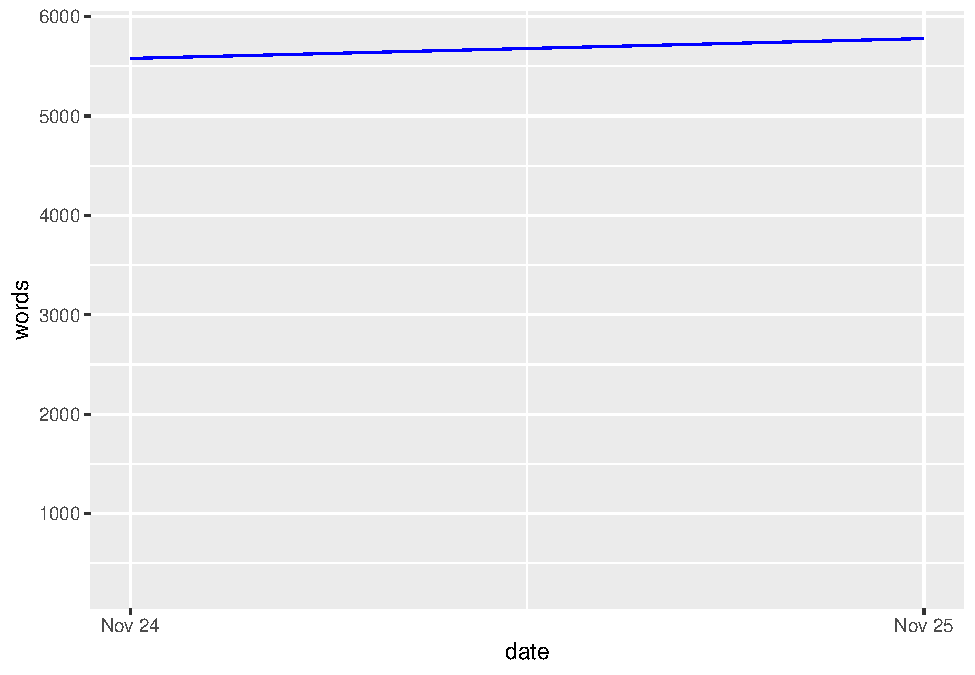
\includegraphics{_main_files/figure-latex/word-count-fig-1.pdf}



\hypertarget{intro-heading}{%
\chapter{Introduction}\label{intro-heading}}

\minitoc 

\hypertarget{additional-ideas}{%
\section{Additional ideas}\label{additional-ideas}}

\hypertarget{general}{%
\subsection{General}\label{general}}

\begin{itemize}
\item
  Explore difference/similarities between the published and unpublished literature, potentially formally, using funnel plots and also by following up preprints to see if they are eventually published. Limit to the date we ran the original search and see if any study included in the study had not been published by the time the review was finished.
\item
  Compare and contrast the codes used to find the AzD cases in the previous study and in this study, potentially with a view to contrasting misclassification between the two.
\item
\end{itemize}

\hypertarget{background}{%
\subsection{Background}\label{background}}

\hypertarget{medrxivr}{%
\subsection{medrxivr}\label{medrxivr}}

\hypertarget{section}{%
\subsection{}\label{section}}

~



\hypertarget{background-heading}{%
\chapter{Background, Theoretical framework, Aims \& Objectives}\label{background-heading}}

\minitoc 

\hypertarget{lay-summary}{%
\section{Lay summary}\label{lay-summary}}

{[}Note: see Section \ref{thesis-structure} for details on the layout of each chapter.{]}

Around 850,000 people in the UK live with dementia, and by 2040, nearly twice as many will have the condition. Despite many promising candidates, no cure for dementia currently exists, meaning the focus is on finding ways to prevent the condition. The best way to do this is to find risk factors (characteristics that influence a person's chance of developing a disease) for dementia that we can easily change. Avoiding a risk factor does not guarantee that a person will not develop dementia but makes it less likely. A key risk factor for dementia may be the levels of lipids (fatty substances such as cholesterol) in a person's blood, though not all existing research agrees. The aim of this thesis is to use all available evidence to assess whether blood lipids levels are in fact a risk factor for dementia.

This introductory chapter provides background information on both dementia and blood lipids, and on the potential link between them. It introduces the theory used to frame the research presented here, and then maps the formal aims and objectives of the research project to the relevant chapters of this thesis. Finally, it summarises the outputs (journal articles, presentations and software) that were created as part of this thesis.

\hypertarget{introduction}{%
\section{Introduction}\label{introduction}}

This chapter provides an overview of the broad context of this thesis, introducing the core concepts used throughout and providing some background on each. It briefly discusses the underlying pathologies and diagnosis of dementia, its public health importance, and the current state of treatment and prevention research. It then provides background on blood lipids and lipid-modifying treatments, and summarises the types of evidence used to examine the effect of these exposures on dementia outcomes.

The chapter introduces evidence synthesis as the key framework used to guide the research presented in the remaining chapters. Finally, it outlines the aims, objectives and structure of this thesis, and briefly summarises the contributions to the scientific literature that arose from this research.

\hypertarget{dementia}{%
\section{Dementia}\label{dementia}}

\hypertarget{underlying-pathologies}{%
\subsection{Definition and underlying pathologies}\label{underlying-pathologies}}

Defined by the Diagnostic and Statistical Manual of Mental Disorders as a ``major neurocognitive disorder'', dementia is a progressive disease which impairs cognitive functions including speech, memory and executive reasoning.\textsuperscript{\protect\hyperlink{ref-edition2013diagnostic}{1}} At advanced stage, the condition causes severe behavioral and personality changes,\textsuperscript{\protect\hyperlink{ref-cerejeira2012}{2}} cumulating in reduced motor control that affects patients ability to swallow or breathe.\textsuperscript{\protect\hyperlink{ref-kumar2013}{3}} The condition has several distinct underlying causes, including Alzheimer's disease and vascular dementia.\textsuperscript{\protect\hyperlink{ref-burns2009}{4}}

Alzheimer's disease is the most common cause of dementia, accounting for approximately 60-80\% of cases. Characterised by substantial cognitive impairment and difficulty with high level executive function to the extent that it interferes with, it is an insidious disease, within initial onset thought to occur up to 15 years prior to symptomatic presentation.\textsuperscript{\protect\hyperlink{ref-robinson2015}{5}} Much remains unknown about Alzheimer's pathogenesis, despite research implicating the ``amyloid hypothesis'',\textsuperscript{\protect\hyperlink{ref-robinson2015}{5}} as a potential mechanism of disease. Under this hypothesis, the build-up of amlyoid plaques (composed mainly of amlyoid-\(\beta\) peptide) and neurofibrillary tangles (composed mainly of tau protein) triggers a range of physiological changes, including inflammation and cell death, that result in cognitive impairment.\textsuperscript{\protect\hyperlink{ref-robinson2015}{5}}

Vascular dementia (VaD) is the second largest underlying pathology of dementia, accounting for \textasciitilde10\% of cases. Vascular dementia is caused by a range of cerebrovascular disorders, and as a result, presentation of symptoms can vary widely.\textsuperscript{\protect\hyperlink{ref-iadecola2013}{6}} Similarly, due to the varied underlying pathophysiology, vascular dementia can onset either quite rapidly following a cerebrovascular event such as a stroke or over a long time-frame due to a series of small infarcts.\textsuperscript{\protect\hyperlink{ref-venkat2015}{7}} Vascular dementia regularly co-occurs in patients with Alzheimer's disease.\textsuperscript{\protect\hyperlink{ref-iadecola2013}{6}} This presentation is described as ``mixed'' dementia,\textsuperscript{\protect\hyperlink{ref-custodio2017}{8}} and occurs in approximately 25\% of cases.\textsuperscript{\protect\hyperlink{ref-burns2009}{4}}

The remaining 10-30\% of cases are caused by other dementia subtypes (e.g.~Lewy body dementia, frontotemporal dementia) or by progression of other neurological diseases (e.g.~Parkinson's disease).\textsuperscript{\protect\hyperlink{ref-burns2009}{4}}

\hypertarget{diagnostic-criteria}{%
\subsection{Diagnostic criteria}\label{diagnostic-criteria}}

Dementia is difficult to diagnose, primarily due to its slow onset, in addition to the confusion of initial symptoms with normal ageing.\textsuperscript{\protect\hyperlink{ref-robinson2015}{5}} Dementia is diagnosed on the basis of behavioral and cognitive changes as assessed by an experienced clinician, using one of several diagnostic criteria.

~





\begin{table}[H]

\caption[Overview of the DSM-5 criteria for dementia and vascular dementia.]{\label{tab:diagnosticCriteria-table}Overview of the DSM-5 criteria for dementia and vascular dementia.\textsuperscript{\protect\hyperlink{ref-edition2013diagnostic}{1}}}
\centering
\begin{threeparttable}
\begin{tabular}[t]{>{\centering\arraybackslash}p{5em}>{\raggedright\arraybackslash}p{27em}}
\toprule
\textbf{Criterion} & \textbf{Major neurocognitive event (previously dementia)}\\
\midrule
\textbf{A} & Evidence of significant cognitive decline from a previous level of performance in one or more cognitive domains:* \newline - Learning and memory \newline - Language \newline - Executive function \newline - Complex attention \newline - Perceptual-motor \newline - Social cognition \newline\\
\midrule
\textbf{B} & The cognitive deficits interfere with independence in everyday activities. At a minimum, assistance should be required with complex instrumental activities of daily living, such as paying bills or managing medications. \newline\\
\midrule
\textbf{C} & The cognitive deficits do not occur exclusively in the context of a delirium. \newline\\
\midrule
\textbf{D} & The cognitive deficits are not better explained by another mental disorder (eg, major depressive disorder, schizophrenia). \newline\\
\bottomrule
\end{tabular}
\begin{tablenotes}
\item[*] From DSM: Evidence of decline is based on concern of the individual, a knowledgeable informant, or the clinician that there has been a significant decline in cognitive function and a substantial impairment in cognitive performance, preferably documented by standardized neuropsychological testing or, in its absence, another quantified clinical assessment.
\end{tablenotes}
\end{threeparttable}
\end{table}

~

One of the most commonly used criteria are those found in the Diagnostic and Statistical Manual of Mental Disorders (DSM) criteria (Table \ref{tab:diagnosticCriteria-table}).\textsuperscript{\protect\hyperlink{ref-edition2013diagnostic}{1}} These criteria are outlined in Table \ref{tab:diagnosticCriteria-table}, and form the broad definition of a dementia diagnoses, supported by a detailed patient history, evidence from carers and family members, and objective assessments of cognitive ability using neurocognitive tests.

Many cognitive assessment tools exist for the purpose of informing a diagnoses of dementia,\textsuperscript{\protect\hyperlink{ref-sheehan2012}{9}} with two of the best known of these being the Mini Mental State Exam (MMSE) and Montreal Cognitive Assessment (MoCA) scale. The distinction between these memory scales and diagnostic criteria presented above should be noted. For example, the MMSE is used to provide evidence for part A of the criteria presented in \ref{tab:diagnosticCriteria-table}. Taken alone, it does not indicate the absence or presence of dementia, instead merely indicating cognitive impairment which could be due to another cause (for example, temporary delirium as a result of an infection or surgery).

Differentiating between the underlying causes of a dementia diagnosis is challenging but necessary, as whether the patient has Alzheimer's disease or vascular dementia will affect expected progression and potential treatment options available (see Section \ref{intro-treatments}). Cause-specific criteria exist for the diagnosis of dementia sub-types. For example, the NINCDS-ADRDA criteria are commonly used to assess patients for Alzheimer's disease,\textsuperscript{\protect\hyperlink{ref-dubois2007}{10}} while vascular dementia is diagnosed using the NINCDS-AIREN criteria.\textsuperscript{\protect\hyperlink{ref-roman1993vascular}{11}}

\hypertarget{public-health-importance}{%
\subsection{Public health importance}\label{public-health-importance}}

Dementia is quickly becoming a critically important public health issue. Despite the age-specific incidence and prevalence of dementia remaining relatively constant over time,\textsuperscript{\protect\hyperlink{ref-prince2016}{12}} an ageing population is set to create a dementia epidemic, particularly in Westernised countries.\textsuperscript{\protect\hyperlink{ref-flier2005}{13}} While approximately 525,000 patients have received a dementia diagnosis, the true number of people currently living with dementia in the UK is thought to be closer to 850,000, with this figure expected to double by 2040.\textsuperscript{\protect\hyperlink{ref-baker2019}{14}} Globally, the prevalence of dementia is expected to reach 75 million by 2030.\textsuperscript{\protect\hyperlink{ref-prince2016}{12}} Dementia is the leading cause of death in the UK, and the only one without a proven cure.

Dementia also has a substantial economic impact. In 2015, the estimated total cost of dementia in England was £24.2 billion. Health care costs alone were £3.8 billion,\textsuperscript{\protect\hyperlink{ref-wittenberg2019}{15}} Globally, the cost of dementia care is expected to rise to \$1tr by 2030.\textsuperscript{\protect\hyperlink{ref-prince2014dementia}{16}}

As such, the urgent need to reduce the burden of dementia, both at the personal and system level, is clear.

\hypertarget{intro-treatments}{%
\subsection{Treatments}\label{intro-treatments}}

Developing treatments for dementia is regularly deemed to be one of the hardest markets in the pharmaceutical world, with trials of seemingly promising therapeutics being regularly abandoned due to futility.\textsuperscript{\protect\hyperlink{ref-cummings2020}{17}}. At present, there are no known curative treatments for dementia, regardless of the underlying cause, though several available therapeutics can help alleviate the symptoms of Alzheimer's disease.

The most common of these are acetylcholinesterase (ACE) inhibitors, which inhibit the degradation of the neurotransmitter acetylcholine by competitively binding the ACE enzyme. Acetylcholine plays a key role in controlling the cholingeric synapses, which are highly concentrated in regions of the brain (such as the neocortex) that control higher level brain functions such as memory and attention.\textsuperscript{\protect\hyperlink{ref-hampel2018}{18}} Commonly prescribed ACE inhibitors include donepezil and galantamine.\textsuperscript{\protect\hyperlink{ref-pariente2008}{19}} ACE inhibitors increase the availability of the neurotransmitter, and has shown clinical effect is easing the behavioural and memory-related symptoms of Alzheimer's disease.\textsuperscript{\protect\hyperlink{ref-marucci2020}{20}} ACE inhibitors represent only a stop-gap treatment, treating the symptoms rather than the underlying pathology which may continue to progress.\textsuperscript{\protect\hyperlink{ref-francis2010}{21}}

\hypertarget{risk-factors}{%
\subsection{Risk factors}\label{risk-factors}}

Given the substantial burden that dementia represents and the absence of any curative therapies, as detailed in the above sections, the assessment of easily modifiable targets for their utility in the prevention of dementia should be prioritized.\textsuperscript{\protect\hyperlink{ref-winblad2016a}{22}} To date, a substantial amount of research has been produced examining putative risk factors for dementia.\textsuperscript{\protect\hyperlink{ref-feingold2000}{23}--\protect\hyperlink{ref-ansteya}{25}}

The benefits of a prevention-based approach based on addressing these risk factors are well-studied. Reducing the prevalence of the seven most important risk factors for dementia (obesity, hypertension,\textsuperscript{\protect\hyperlink{ref-hughes2020association}{26}} diabetes, smoking, physical inactivity, and low educational attainment) by 10-20\% per decade is estimated to result in a reduction in dementia prevalence of 8-15\% by 2050.\textsuperscript{\protect\hyperlink{ref-norton2014potential}{27}}

In this context, lipid levels represent a promising target for preventative treatment, due to the ready availability of lipid-modifying treatments which could be repurposed.\textsuperscript{\protect\hyperlink{ref-pushpakom2019a}{28}} Determining whether variations in lipid levels are causative for dementia may prove critical in reducing the future burden of the condition.

This thesis will focus on blood lipids as the primary risk factor of interest. The next section provides an overview of blood lipid fractions and therapeutic interventions that modify them, while Section \ref{evidence-association} provides an overview of the existing evidence for an association between lipids and dementia outcomes.

\hypertarget{serum-lipids}{%
\section{Serum lipids}\label{serum-lipids}}

\hypertarget{intro-lipid-fractions}{%
\subsection{Lipid fractions}\label{intro-lipid-fractions}}

The blood lipid profile contains a range of component parts, or fractions. However, this thesis will only consider the two most important fractions, trigylcerides (TG) and cholesterol, which are either absorbed from food (exogenous lipids) or produced internally (endogenous lipids).\textsuperscript{\protect\hyperlink{ref-feingold2000}{23}}

Triglycerides are the simplest and most common type of lipids found across the body. They are used to store unused calories from food, and to move energy around the body.\textsuperscript{\protect\hyperlink{ref-laufs2020}{29}} In contrast, cholesterol is primarily used to create cell walls and certain sex hormones.\textsuperscript{\protect\hyperlink{ref-zampelas2019}{30}} As lipids are not water soluble, within the blood stream, cholesterol is transported in lipoprotein structures of varying densities. Low-density-lipoprotein cholesterol (LDL-c), commonly know as the ``bad'' cholesterol, transports fat to cells, acting as an energy conveyor. In contrast, High density-lipoprotein cholesterol (HDL-c), transports cholesterol to the liver to be broken down and excreted.\textsuperscript{\protect\hyperlink{ref-feingold2000}{23}}

In addition to the individual fractions, total serum cholesterol (TC) is a commonly-used summary measure to estimate the total amount of lipid present in the blood. The measure is derived from measurements of the individual HDL-c, LDL-c and TG levels using the Friedwald formula:\textsuperscript{\protect\hyperlink{ref-friedewald1972}{31}}

\[TC \approx LDLc + HDLc + kTG\]
where \(k\) is 0.20 if measurements are in milligrams per decilitre (\emph{mg/dl}) and 0.45 if measured in millimole per litre (\emph{mmol/l}).

Widely-used ranges for the acceptable levels of different types of lipids are based on the National Cholesterol Education Program (NCEP)\textsuperscript{\protect\hyperlink{ref-national2002third}{32}}, and are outlined in Table \ref{tab:lipidLevels-table}.

~





\begin{table}[H]

\caption[Classification of blood lipid levels]{\label{tab:lipidLevels-table}Classification of blood lipid levels according to the National Cholesterol Education Program guidelines.\textsuperscript{\protect\hyperlink{ref-national2002third}{32}}}
\centering
\begin{tabular}[t]{lll}
\toprule
\textbf{Fraction} & \textbf{Measure (mg/dL)} & \textbf{Classification}\\
\midrule
 & <100 & Optimal\\
\cmidrule{2-3}
 & 100-129 & Near/above optimal\\
\cmidrule{2-3}
 & 130-159 & Borderline high\\
\cmidrule{2-3}
 & 160-189 & High\\
\cmidrule{2-3}
\multirow{-5}{*}{\raggedright\arraybackslash LDL cholesterol} & >190 & Very high\\
\cmidrule{1-3}
 & <40 & Low\\
\cmidrule{2-3}
\multirow{-2}{*}{\raggedright\arraybackslash HDL cholesterol} & >60 & High\\
\cmidrule{1-3}
 & <150 & Normal\\
\cmidrule{2-3}
 & 150-199 & Borderline high\\
\cmidrule{2-3}
 & 200-499 & High\\
\cmidrule{2-3}
\multirow{-4}{*}{\raggedright\arraybackslash Triglycerides} & >500 & Very high\\
\cmidrule{1-3}
 & <200 & Desirable\\
\cmidrule{2-3}
 & 200-239 & Borderline high\\
\cmidrule{2-3}
\multirow{-3}{*}{\raggedright\arraybackslash Total cholesterol} & >240 & High\\
\bottomrule
\end{tabular}
\end{table}

~

Elevated LDL-c in the bloodstream, a condition also known as hypercholesterolaemia or hyperlipidaemia,\textsuperscript{\protect\hyperlink{ref-nelson2013}{33}} can lead to atherosclerosis,\textsuperscript{\protect\hyperlink{ref-libby2019}{34}} the build-up of fatty deposits in the blood vessels. These deposits constrict blood flow and can lead to vascular complications. Alternatively, part of the deposit can detach from the artery walls, forming a clot that can lead to a heart attach or stroke.\textsuperscript{\protect\hyperlink{ref-libby2019}{34}} Globally, the prevalence of elevated cholesterol was estimated by the World Health Organization to be approximately 40\%.

\hypertarget{intro-statins}{%
\subsection{Statins}\label{intro-statins}}

Statins are a commonly prescribed method of lipid regulation.\textsuperscript{\protect\hyperlink{ref-collins2016}{35}} Statins inhibit the conversion of 3-hydroxy-3-methylglutaryl-coenzyme-A (HMG-CoA) into mevalonate, by competitively binding with HMG-CoA reductase (HMG-CoA-R). This conversion is a key rate-limiting step in the cholesterol biosynthesis pathway (see Figure \ref{statin-mechanisam}), enabling statins to reduce effectively the production of LDL cholesterol.

~





\begin{figure}[H]

{\centering 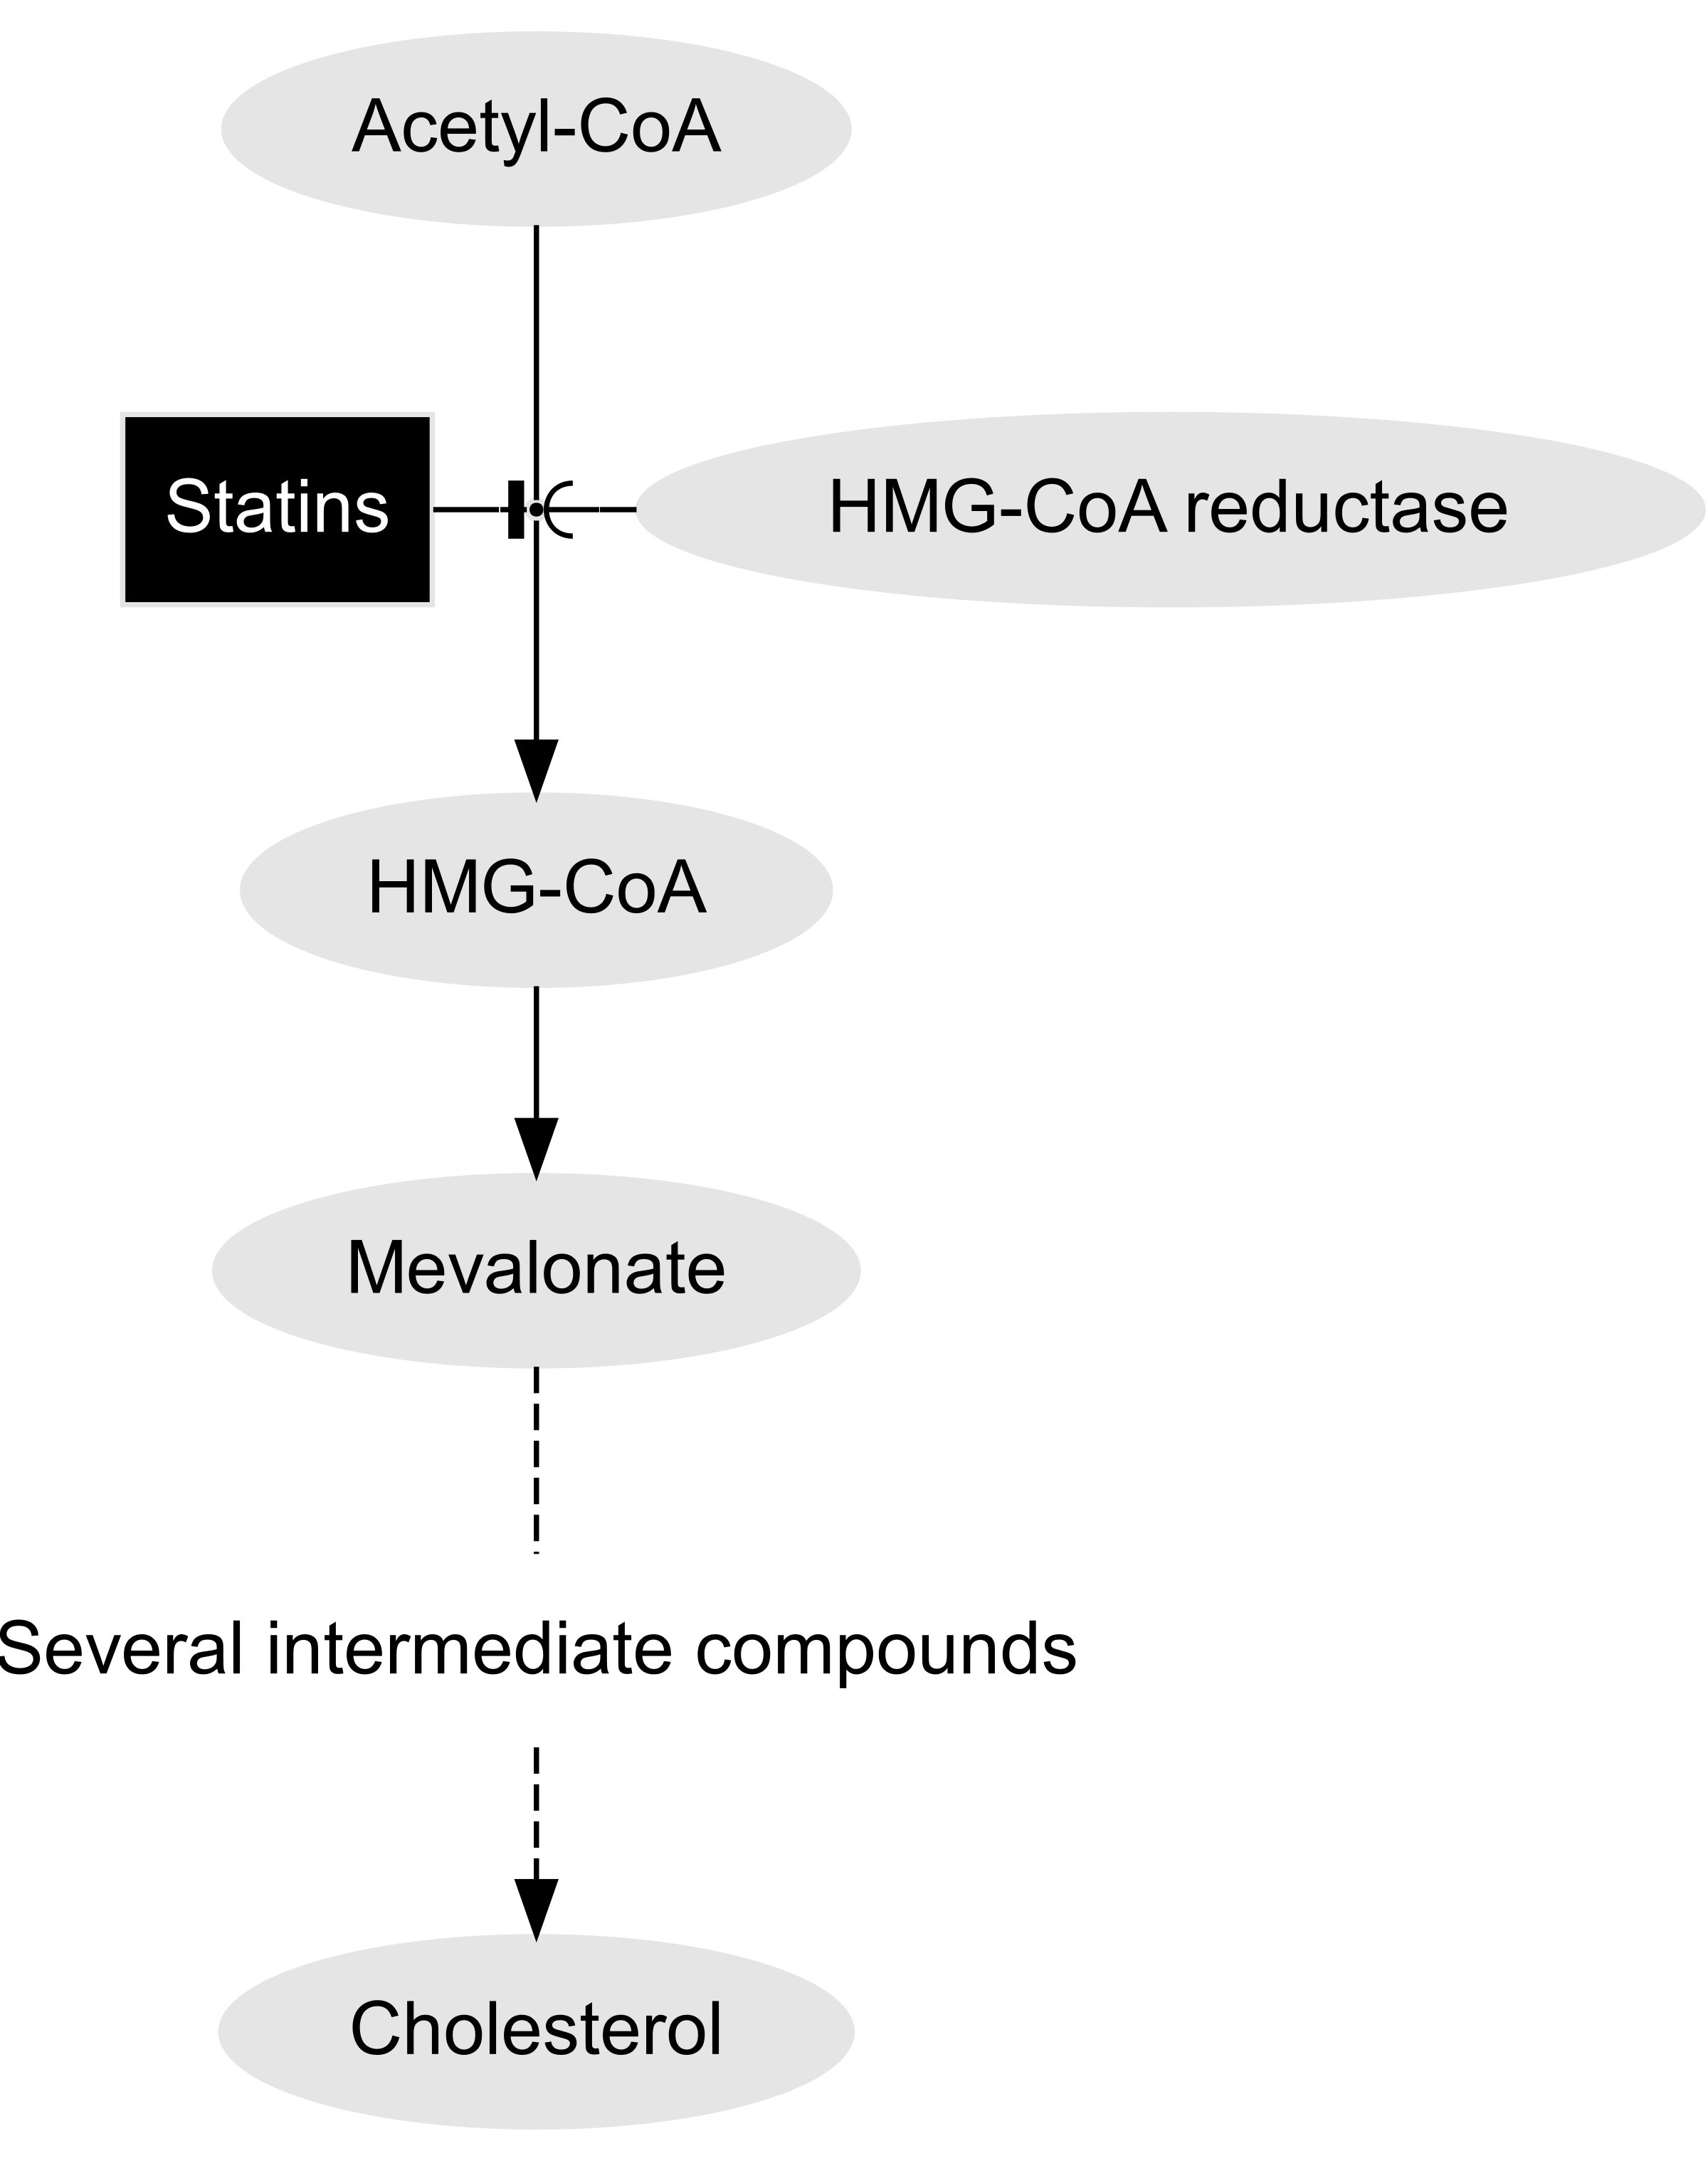
\includegraphics[width=0.5\linewidth]{figures/background/statinPath} 

}

\caption[Statin mechanism of action]{Overivew of statins mechanism of action, inhibiting HMG-CoA reductase which controls the conversion of HMG-CoA to mevalonate, the rate-limiting step in cholesterol biosynthesis.}\label{fig:statin-mechanisam}
\end{figure}

~

Several statin treatments have been widely available for some time (see Table \ref{tab:statinOverview-table}). Depending on the statin and dosage prescribed, the average reduction in LDL-c concentrations ranges from 15\% with low-intensity regimen (e.g.~ravastatin 5 mg/day) up to 60\% with a high-intensity regimen (e.g.~rosuvastatin 80 mg/day).\textsuperscript{\protect\hyperlink{ref-collins2016a}{36},\protect\hyperlink{ref-law2003}{37}} Statins also vary with regard to their lipophilicity (the extent to which they are lipid soluble), affecting their localisation within the body, with hydophilic statins being concentrated in the liver and lipophilic statins circualting more widely.\textsuperscript{\protect\hyperlink{ref-schachter2005}{38}} This may create a divide in the pleiotropic affects of statins with differing lipophilicity, particularly given the ability of lipophilic statins to permeate the blood brain barrier.\textsuperscript{\protect\hyperlink{ref-sierra2011}{39}}

~





\begin{table}[H]

\caption[Overview of common statins]{\label{tab:statinOverview-table}Overview of commonly-prescribed statins, summarising their approval date (US), properties and lipid-lowering effect.}
\centering
\begin{tabular}[t]{>{\centering\arraybackslash}p{6em}>{\centering\arraybackslash}p{6em}>{\centering\arraybackslash}p{6em}>{\centering\arraybackslash}p{6em}>{\centering\arraybackslash}p{7.6em}}
\toprule
\textbf{Name} & \textbf{Brand name} & \textbf{Year approved} & \textbf{Properties} & \textbf{Lipid-lowering effect}\\
\midrule
\textbf{Atorvastatin} & Lipitor & 1996 & Lipophilic & +++\\
\midrule
\textbf{Pravastatin} & Lipostat & 1989 & Hydrophilic & +\\
\midrule
\textbf{Rosuvastatin} & Crestor & 2003 & Hydrophilic & ++++\\
\midrule
\textbf{Simvastatin} & Zocor & 1992 & Lipophilic & ++\\
\bottomrule
\end{tabular}
\end{table}

~

\hypertarget{other-lipid-regulating-agents-lra}{%
\subsection{Other lipid regulating agents (LRA)}\label{other-lipid-regulating-agents-lra}}

There are several other interventions that can be used to modify a persons lipid profile, which each acting in slightly different ways (Table \ref{tab}). However, in general, these treatments are either used as adjunct (additional) treatments with statins therapy or are used in situations where statins are contra-indicated or not tolerated.

The most commonly used non-statin therapeutic is ezetimibe,\textsuperscript{\protect\hyperlink{ref-kosoglou2005}{40}} which prevents intestinal absorption of cholesterol. However, when used alone, it has a limited LDL-c lowering effect, leading to the creation of combined statin/ezetimibe therapies (both compounds contained in a single pill, as opposed to complimentary treatments).\textsuperscript{\protect\hyperlink{ref-genest2006}{41}}

Fibrates provide a second example of non-statin therapy. They are used to treat hypertriglyceridaemia by reducing production of triglyceride carrying compounds in the liver. They are commonly used in patients with mixed hyperlipidaemia if treatment with statins has failed to sufficiently control cholesterol levels.

Finally, PCSK9 inhibitors (or PCSK9i) are a relatively new treatment with strong lipid lowering effects, lauded as a potential alternative to statins.\textsuperscript{\protect\hyperlink{ref-chaudhary2017}{42}} Their mechanism of action is to bind to and inhibit PCSK9, which breaks down LDL-c receptors on the surface of the liver, thus allowing more LDL-c to be internalised and broken down.

Other therapies targeting triglycerides exist, including nicotinic acids\textsuperscript{\protect\hyperlink{ref-mckenney2004new}{43}} and omega-3-fatty acids,\textsuperscript{\protect\hyperlink{ref-skulas-rayannc.2019}{44}} but they far less effective in LDL-c lowering than the therapies described above.

~



\begin{table}[H]

\caption{\label{tab:lipidTreatments-table}Summary of available treatments for hyperlipidaemia.}
\centering
\begin{tabular}[t]{>{\raggedright\arraybackslash}p{8em}>{\raggedright\arraybackslash}p{8em}>{\raggedright\arraybackslash}p{8em}>{\raggedright\arraybackslash}p{8em}}
\toprule
\textbf{Treatment} & \textbf{Effect} & \textbf{Mechanism of action} & \textbf{Examples}\\
\midrule
\textbf{HMG CoA reductase inhibitors (statins)} & Lowers LDL-c \& TG \newline Raises HDL-c & Inhibits cholesterol biosynthesis pathway in the liver & Atorvastatin, \newline Simvastatin, \newline Pravastatin\\
\midrule
\textbf{Ezetimibe} & Lowers LDL-c & Prevents absorption of cholesterol from diet & \\
\midrule
\textbf{Bile acide sequestrants} & Lowers LDL-c & Prevent bile acid reabsorption in the gastro-intestinal tract, increasing conversion of cholesterol to bile acids & Colestipol\\
\midrule
\textbf{Proprotein convertase subtilisin kexin 9 (PCSK9) inhibitors} & Lowers LDL-c & Bind to PSCK9 protein, preventing it from breaking down LDL receptors on heptatic cells, increasing cholesterol uptake & Evolocumab, \newline Alirocumab\\
\bottomrule
\end{tabular}
\end{table}

~

\hypertarget{evidence-association}{%
\section{Evidence for the association between blood lipids and dementia}\label{evidence-association}}

This section provides an overview of the varying sources of evidence on the relationship between blood lipid levels and dementia risk.

\hypertarget{basic-science}{%
\subsection{Basic science}\label{basic-science}}

A role for lipids in the aetiology of the dementia is supported by both genetic linkage studies and functional cell biology studies. The generation of the amyloid plaques found in the brains of Alzheimer's patients is cholesterol dependent,,\textsuperscript{\protect\hyperlink{ref-burns2003}{45},\protect\hyperlink{ref-mizuno1999}{46}} while the most established genetic risk factor for late-onset dementia, apolipoprotein E (ApoE), is involved in cerebral cholesterol transport. Several other genes involved in cholesterol transport have also been found to be associated with increased AD susceptibility.\textsuperscript{\protect\hyperlink{ref-beecham2014}{47}--\protect\hyperlink{ref-meng2007}{49}}

Despite these results, evidence from the diverse range of epidemiological studies on this topic has been inconclusive.

\hypertarget{observational-studies}{%
\subsection{Observational studies}\label{observational-studies}}

By far the largest source of evidence on the relationship between comes from observational designs. Several studies have examined the relationships between concentrations of serum lipids (total cholesterol (TC), low density lipoprotein cholesterol (LDL-c), high density lipoprotein cholesterol (HDL-c) and triglycerides) and both Alzheimer's disease and vascular dementia and reported extremely varied results. In some studies, a high serum cholesterol concentration has been found to be associated with an increase in susceptibility to AD,\textsuperscript{\protect\hyperlink{ref-kivipelto2002}{50}--\protect\hyperlink{ref-whitmer2005}{54}} however others have shown no association,\textsuperscript{\protect\hyperlink{ref-li2005a}{55}--\protect\hyperlink{ref-tan2003a}{58}} or a reduced susceptibility.\textsuperscript{\protect\hyperlink{ref-mielke2005}{59},\protect\hyperlink{ref-reitz2004a}{60}} With regards vascular dementia, decreased levels of HDL-c appear to be associated with increased risk,\textsuperscript{\protect\hyperlink{ref-reitz2004a}{60}} while for LDL-c, studies have reported both positive and negative associations.\textsuperscript{\protect\hyperlink{ref-reitz2004a}{60},\protect\hyperlink{ref-moroney1999}{61}}

Several previous systematic review of observational studies examining the effect of lipids\textsuperscript{\protect\hyperlink{ref-anstey}{62}} and lipid-regulating agents\textsuperscript{\protect\hyperlink{ref-chu2018b}{63},\protect\hyperlink{ref-poly2020c}{64}} on dementia outcomes have been performed. However, these reviews have several limitations. Many did not consider grey literature sources (see Section \ref{diverse-sources-preprints}). Additionally, many of the reviews of observational studies did not perform any risk-of-bias assessment\textsuperscript{\protect\hyperlink{ref-chu2018b}{63}} or used an outdated assessment tool.\textsuperscript{\protect\hyperlink{ref-anstey}{62},\protect\hyperlink{ref-poly2020c}{64}}

\hypertarget{randomised-controlled-trials}{%
\subsection{Randomised controlled trials}\label{randomised-controlled-trials}}

In terms of the central research of this thesis, RCTs of statin therapy can be used to provide indirect evidence for the effect of reducing blood LDL-c levels on dementia risk.

However, RCTs may be infeasible if the outcome of interest is one with a long prodomal period, such as dementia (see Section \ref{underlying-pathologies}), as they would require extremely long and costly follow-up.\textsuperscript{\protect\hyperlink{ref-ritchie2015}{65}} It is no surprise then that the two previous trials providing evidence on the effect of statins on dementia risk, identified by a recent Cochrane review,\textsuperscript{\protect\hyperlink{ref-mcguinness2016a}{66}} are in fact trials of statins for the prevention of coronary related outcomes.

While being widely cited, these studies have major limitations that reduce their utility as a source of evidence on the effect of statin treatment on in assessing the impact of lipid-lowering treatment on dementia risk. Firstly, there was no clinical cognitive evaluation of patients to determine a dementia outcome. One of the trials, the Prospective Study of Pravastatin in the Elderly (PROSPER) trial,\textsuperscript{\protect\hyperlink{ref-trompet2010}{67}} reported not on dementia outcomes but on the change in cognitive scores over a mean of 3.2 years. As highlighted in Section \ref{diagnostic-criteria}, a ``change in score'' alone is insufficient to diagnose a dementia outcome. The second trial, the Medical Research Council/British Health Foundation Protection Study,\textsuperscript{\protect\hyperlink{ref-2002}{68}} found no effect of simvastatin on dementia (OR: 1.00, 95\% CI: 0.61-1.65), but did not report how the outcome was assessed/recorded within the trial.

Additionally, the two trials did not make any effort to assign an underlying pathology to each case, instead reporting an all-cause dementia outcome. As discussed in Section \ref{underlying-pathologies}, the different underlying pathology of dementia have different mechanisms of action, and so it is not gauranteed that the effect of statins would be consistent across them.

Both trials were also limited by the relatively short follow-up period examined, expected when the primary outcome of the trials were coronary related conditions rather than dementia.\textsuperscript{\protect\hyperlink{ref-trompet2010}{67},\protect\hyperlink{ref-2002}{68}} The PROSPER trial had a mean follow-up of 3.2 years, while the MRC/BHF Protection Study estimated risk at 5 years of follow-up. Given the long lag time between non-symptomatic onset of dementia and clinical presentation, it is likely that these durations are insufficient to fully capture the onset of dementia. Finally, as they included only patients at high vascular risk, their generalisability to other settings is limited.\textsuperscript{\protect\hyperlink{ref-mcguinness2016b}{69}}

\hypertarget{mendelian-randomisation}{%
\subsection{Mendelian randomisation}\label{mendelian-randomisation}}

Newer methodological approaches, such as Mendelian randomisation (MR),\textsuperscript{\protect\hyperlink{ref-daveysmith2014}{70}} have also been used to examine the effect of varying lipid levels on dementia risk in an effort to combat the risk of reverse causation and residual confounding inherent to observational studies.\textsuperscript{\protect\hyperlink{ref-greenland2000}{71}} In brief, MR uses genetic variants that are both strongly associated with the exposure of interest and are independent from potential confounders to strengthen causal inference.\textsuperscript{\protect\hyperlink{ref-daveysmith2014}{70}} The analytic method relies on several assumptions about the instrumental variable (IV),\textsuperscript{\protect\hyperlink{ref-davies2018}{72}} namely that:

\begin{enumerate}
\def\labelenumi{\arabic{enumi}.}
\tightlist
\item
  the IV is associated with the exposure of interest (the relevance assumption);
\item
  the IV and outcome do not share a common cause (the independence assumption); and
\item
  the IV does not affect the outcome other than via the exposure (the exclusion restriction assumption).
\end{enumerate}

Recent MR studies indicated that genetically determined low levels of LDL-c may cause a reduction in AD risk.\textsuperscript{\protect\hyperlink{ref-larsson2017c}{73},\protect\hyperlink{ref-ostergaard2015}{74}} However, the effect was attenuated in sensitivity analysis that exclude the region surrounding the ApoE gene, the strongest known risk factor for Alzheimer's disease.\textsuperscript{\protect\hyperlink{ref-kim2009}{75}} Inclusion of ApoE4 variants invalidates the exclusion restriction criteria (Assumption 3, above), as the risk reduction observed may be driven by variants in this region via a pathway independent of lipid levels. This was supported by further MR studies where \emph{ApoE4} variants were intentionally excluded.\textsuperscript{\protect\hyperlink{ref-benn2017}{76}}

Despite the increasing number of MR studies examining this topic, no systematic review of this study design as a source of evidence has been performed.

~

In summary, multiple sources of evidence exist on the relationship between statins and dementia. In the next section, I introduce the synthesis of diverse sources of evidence as the theoretical framework used in this thesis.

\hypertarget{theoretical-framework-evidence-synthesis}{%
\section{Theoretical framework: Evidence synthesis}\label{theoretical-framework-evidence-synthesis}}

Evidence synthesis is the process of finding and integrating information from several sources to examine a research question.\textsuperscript{\protect\hyperlink{ref-donnelly2018a}{77}} A common tyoe of evidence synthesis is a systematic review, either with or without a meta-analysis.\textsuperscript{\protect\hyperlink{ref-chandler2019chapter}{78}}

The results of an evidence synthesis exercise can be used to provide a more definitive answer to that question or, failing that, to highlight gaps in the existing evidence base. The ability to identify these gaps is particularly useful in guiding future research to address questions that have yet to be answered.

This thesis seeks to use an evidence synthesis framework to assess the effect of lipids, and treatments that influence lipid levels, on dementia outcomes.
Specifically, this thesis considers three concepts within the umbrella term of evidence synthesis:

\begin{itemize}
\tightlist
\item
  Inclusion of preprints
\item
  Triangulation across evidence sources
\item
  Individual patient data meta-analysis
\end{itemize}

These three elements are expanded on below and are used to frame the research presented in the subsequent Chapters.

\hypertarget{diverse-sources-preprints}{%
\subsection{Inclusion of preprints}\label{diverse-sources-preprints}}

The importance of including grey (or gray) literature in systematic reviews is widely acknowledged. Meta-research studies have demonstrated that systematic reviews excluding grey literature sources overestimate the effect of interventions.\textsuperscript{\protect\hyperlink{ref-conn2003}{79}--\protect\hyperlink{ref-hopewell2007}{81}} Common, well-accepted forms of grey literature include conference abstracts and theses.\textsuperscript{\protect\hyperlink{ref-lefebvre2019searching}{82}}

A important developing source of grey literature are preprints. Defined by the Committee on Publication Ethics (COPE) as `scholarly manuscript{[}s{]} posted by the author(s) in an openly accessible platform, usually before or in parallel with the peer review process'\textsuperscript{\protect\hyperlink{ref-committeeonpublicationethicscope2018}{83}}, preprints serve several purposes. They are used to establish primacy when submitting to a journal where the peer-review process may take several months,\textsuperscript{\protect\hyperlink{ref-vale2016}{84}} to rapidly disseminate research findings, as occurred during the COVID-19 pandemic,\textsuperscript{\protect\hyperlink{ref-fraser2020a}{85}} and to make available publications that may not have been accepted elsewhere in an attempt to combat publication bias or the ``file-drawer'' effect.\textsuperscript{\protect\hyperlink{ref-rosenthal1979}{86}}

One of the major criticisms of using preprints as an evidence source is that they have not yet undergone formal peer review.\textsuperscript{\protect\hyperlink{ref-maslove2018}{87},\protect\hyperlink{ref-schalkwyk2020}{88}} However, this approach assigns substantial weight to peer-review as a indicator of ``quality'', and is at odds with the acceptance of non-reviewed conference proceedings as an evidence source.\textsuperscript{\protect\hyperlink{ref-lefebvre2019searching}{82},\protect\hyperlink{ref-mahood2014}{89}} The argument for including preprints as an evidence source is further strengthened by results that demonstrate preprinted studies seldom change following peer review. Meta-studies of the concordance between preprinted and published studies showed that results were broadly comparable between the two, indicating that while the numerical results may change, the overall interpretation of the results were consistent in the majority of cases.\textsuperscript{\protect\hyperlink{ref-shi2021a}{90}--\protect\hyperlink{ref-nicholson2021}{92}} This indicates that preprints should be considered a reliable reflection of a given study.

In this thesis, preprints are considered an important source of evidence, in contrast to previous reviews on this topic. However, as with many sources of grey literature,\textsuperscript{\protect\hyperlink{ref-mahood2014}{89}} there are several logistical issues with carrying out systematic searches in preprint repositories. As such, to enable the inclusion of preprints in the systematic review described in Chapter \ref{sys-rev-heading}, a new tool addressing these issues is presented in Chapter \ref{sys-rev-tools}.

\hypertarget{intro-triangulation}{%
\subsection{Triangulating across study designs}\label{intro-triangulation}}

As illustrated in Section \ref{evidence-association}, several diverse epidemiological methods have been used to examine the effect of varying blood lipid levels on dementia risk. However, each method is limited by its own biases. Aetiological triangulation is a developing evidence synthesis method that seeks to exploit these inherent differences in study design, and as a result, in biases.\textsuperscript{\protect\hyperlink{ref-lawlor2016a}{93}} If several sources of evidence are available and point towards identical conclusions about an exposure-outcome relationship, and these sources are at risk of unrelated biases, this strengthens our confidence in the result. The ideal scenario is where predicted sources of bias are likely to be in competing directions, strengthen the effect of the exposure and the other to attenuate it.\textsuperscript{\protect\hyperlink{ref-lawlor2016a}{93}} As such, triangulating these results can provides us a middle-ground between the competing directions of bias. A triangulation approach can also prove useful in a prospective manner, helping to design new studies that are at risk of different sources of bias to that already available from the published literature.\textsuperscript{\protect\hyperlink{ref-munafo2018}{94}}

This thesis seeks to apply a triangulation approach to provide the best available evidence on the effect of lipids, and lipid regulating agents, on dementia outcomes.

All existing evidence, regardless of study design, is first identified by the by the systematic review presented in Chapter \ref{sys-rev-heading}. Risk-of-bias assessment using a domain-based tool is already a recommended part of the systematic review process, but is particularly important to a triangulation exercise.\textsuperscript{\protect\hyperlink{ref-Pagen71}{95}--\protect\hyperlink{ref-mcguinness2018}{97}} As such, a core component of the review is a comprehensive domain-based risk-of-bias assessment for all included studies.

Finally all evidence, both pre-existing and produced as part of this thesis (Chapter \ref{cprd-analysis-heading} and \ref{ipd-analysis-heading}), are triangulated in Chapter \ref{dicussion-heading}.

\hypertarget{individual-patient-data-meta-analysis}{%
\subsection{Individual patient data meta-analysis}\label{individual-patient-data-meta-analysis}}

Individual patient data meta-analyses are commonly held to represent the gold standard in evidence synthesis methodology.\textsuperscript{\protect\hyperlink{ref-riley2010}{98},\protect\hyperlink{ref-stewart1993}{99}} IPD methods seek to obtain the raw data from each study identified in a systematic review, rather than basing the meta-analysis on summary results extracted from the literature.\textsuperscript{\protect\hyperlink{ref-riley2010}{98}}

In the context of this thesis, if lipids are found to have a causal role in development of dementia, evidence-based preventative strategies would be best informed by identifying the types of individuals who are most likely to receive benefit from treatment with lipid-modifying agents.\textsuperscript{\protect\hyperlink{ref-arain2009}{100}--\protect\hyperlink{ref-mccartney2016}{102}} However, if primary studies do not present results stratified by covariates of interest, meta-analyses of summary-level data on this topic often have limited ability to examine research questions related to exposure-covariate interactions.\textsuperscript{\protect\hyperlink{ref-riley2010}{98}} In terms of this thesis, patient sex is considered to be of particular interest.\textsuperscript{\protect\hyperlink{ref-arain2009}{100},\protect\hyperlink{ref-letenneur1999}{103}}

An IPD meta-analysis of lipid levels on dementia outcomes would overcome this limitation of summary-level data, as access to the raw data allows for an analysis that investigates these interactions.\textsuperscript{\protect\hyperlink{ref-riley2020}{104}} This approach has the added benefit of allowing a common set of inclusion criteria and statistical model to be applied across all datasets, potentially eliminating some important sources of heterogeneity.\textsuperscript{\protect\hyperlink{ref-stewart2002}{105}}

Despite their advantages, IPD meta-analysis are rarely performed.\textsuperscript{\protect\hyperlink{ref-tugwell2010}{106}} Factors limiting their uptake include the increased time and effort they require when compared to a summary-level analysis, and the low success rate associated with obtaining the raw data.\textsuperscript{\protect\hyperlink{ref-nevitt2017a}{107},\protect\hyperlink{ref-ventresca2020}{108}} The data underlying primary studies are frequently not publicly available,\textsuperscript{\protect\hyperlink{ref-alsheikh-ali2011}{109},\protect\hyperlink{ref-federer2018a}{110}} and the availability of data ``available on request from authors'' declines rapidly over time.\textsuperscript{\protect\hyperlink{ref-vines2014}{111}} Several systematic barriers to open data sharing have been identified\textsuperscript{\protect\hyperlink{ref-vanpanhuis2014a}{112}}. Of particular concern for biomedical IPD analyses are legal issues surrounding the sharing of medical data, motivated by concerns around patient privacy.\textsuperscript{\protect\hyperlink{ref-wartenberg2010}{113}}

In response to these limitations, new collaborative initiatives have developed to enable rapid access to relevant data in a secure supported workshop. The most import in relation to this thesis is the Dementia Platform UK (DPUK),\textsuperscript{\protect\hyperlink{ref-bauermeister2020}{114}} which aims to provide access to several dementia-related datasets via a single simplified application process.

I will will attempt to obtain the raw data from relevant primary studies identified by the systematic review in Chapter \ref{sys-rev-heading}. Any data obtained will be combined with that available from the DPUK portal as part of an individual participant data meta-analysis in Chapter \ref{ipd-analysis-heading}, enabling the assessment of the effect of lipids on dementia stratified by key variables such as sex.

\hypertarget{thesis-overview}{%
\section{Thesis overview}\label{thesis-overview}}

\hypertarget{aims-and-objectives}{%
\subsection{Aims and objectives}\label{aims-and-objectives}}

The over-arching aim of this thesis is to explore the relationship between blood lipid levels, and by extension treatments that modify blood lipid levels such as statins, and the subsequent risk of dementia and related outcomes

The specific research objectives that this thesis seeks to address are:

\begin{itemize}
\tightlist
\item
  To create a tool that allows for the inclusion of health related preprints in evidence syntheses in a systematic and reproducible manner
\item
  To review all available evidence across multiple diverse study designs to assess the effect of lipids and lipid regulating agents on dementia risk
\item
  To examine whether there is evidence for an effect of lipid-regulating agents on dementia and related outcomes in a large scale population-based cohort, the Clinical Practice Research Datalink (CPRD)
\item
  To meta-analyse raw dementia-related datasets as part of a individual participant data (IPD meta-analysis) to produce evidence on exposure-covariate interactions
\end{itemize}

\hypertarget{thesis-structure}{%
\subsection{Structure}\label{thesis-structure}}

Chapters are self-contained, presenting the methods and results of that specific research project. They are bookended by introductory and discussion sections which place the methods and results in context. Each chapter is prefaced by a ``Lay'' or plain English summary, developed with input from the Patient and Public Advisory Group (see Section \ref{disc-PPI} for a discussion of the group's involvement and Appendix \ref{appendix-ppi} for more detail on the group).

\begin{itemize}
\tightlist
\item
  \textbf{Chapter \ref{background-heading}:} Background information on dementia and blood lipid levels. This chapter provides an introduction to the topics covered in this thesis to non-subject area experts, and discusses the motivation for the remainder of the thesis.
\item
  \textbf{Chapter \ref{sys-rev-tools-heading}:} This Chapter introduces a new tool, \texttt{medrxivr}, which was used to developed to allow for systematic searches of the health-related preprint repositories.
\item
  \textbf{Chapter \ref{sys-rev-heading}:} This Chapter describes a comprehensive systematic review and meta-analysis of all available evidence on the effect of blood lipids, and interventions that modified blood lipids, on dementia outcomes.
\item
  \textbf{Chapter \ref{cprd-analysis-heading}:} This Chapter examines the relationship between lipid-regulating agent use and dementia outcomes in the Clinical Practice Research Datalink, a large primary care electronic health record database.
\item
  \textbf{Chapter \ref{ipd-heading}:} This Chapter describes an individual patient data analysis of several longitudinal cohort studies to describe the relationship between blood serum lipids and dementia outcomes, stratified by important covariates such as sex.
\item
  \textbf{Chapter \ref{discussion-heading}}: This Chapter integrates the diverse evidence identified by, and produced as part of, this thesis. The overall strengths and weaknesses of this project are discussed in detail, and further avenues of research are suggested.
\end{itemize}

An overview of how all research studies in this thesis can be found in Table \ref{tab:thesisOverview-table}

\blandscape





\begin{table}[H]

\caption[Summary of studies included in this thesis]{\label{tab:thesisOverview-table}Summary of studies included in this thesis, and used as evidence sources in the triangulation exercise performed in Chapter \ref{discussion-heading}. Note, Chapter \ref{sys-rev-tools-heading} is intentionally not included in this table, as it describes a tool rather than a research study.}
\centering
\begin{tabular}[t]{>{\raggedright\arraybackslash}p{6em}>{\raggedright\arraybackslash}p{16em}>{\raggedright\arraybackslash}p{7em}>{\raggedright\arraybackslash}p{7em}>{\raggedright\arraybackslash}p{16em}}
\toprule
\textbf{Chapter} & \textbf{Research Question} & \textbf{Exposure/ Intervention} & \textbf{Outcome} & \textbf{Contibution to evidence synthesis framework}\\
\midrule
Chapter 3 & Based on the available evidence; \newline (i) are lipid fractions associated with subsequent dementia risk, stratified by subtype? \newline (ii) Are lipid regulating agents associated with subsequent dementia risk, stratified by subtype? \newline & Lipids (HDL-c, LDL-c, TC, TG), \newline \newline Lipid regulating agents (statins, ezetimibe, fibrates, etc.) & Dementia, stratified by subtype & Provides overview of existing evidence\\
\midrule
Chapter 4 & Are lipid regulating agents associated with dementia risk in a large scale electonic health record database? \newline & Seven classes of lipid regulating agents & Dementia, stratified by subtype & Provides additional observational data on vascular dementia (under-represented in the literature) \newline \newline Provides a source of observational evidence created using a method with distinct sources of bias to those identified by the systematic review\\
\midrule
Chapter 5 & Are lipid levels associated with dementia risk in an individual participant data meta-analysis? \newline & Lipids (HDL-c, LDL-c, TC, TG) & Dementia, stratified by subtype & Provides additional evidence from unanalysed datasets \newline \newline Allows for stratification of effect by variables of interest (e.g. sex)\\
\bottomrule
\end{tabular}
\end{table}

\elandscape

\hypertarget{thesis-output}{%
\section{Outputs from this thesis}\label{thesis-output}}

The outputs of this thesis are detailed below, and include peer-reviewed papers, presentations, and open-source evidence synthesis tools.

\hypertarget{contributions-to-the-scientific-literature}{%
\subsection{Contributions to the scientific literature}\label{contributions-to-the-scientific-literature}}

During the course of this thesis, I have made several contributions to the scientific literature. Those arising from or directly related to the contents of this submission are presented below.

~

\emph{\textbf{McGuinness, L. A.}, and L Schmidt. (2020) medrxivr: Accessing and searching medRxiv and bioRxiv preprint data in R. Journal of Open Source Software 5.54 2651. DOI: \href{https://doi.org/10.21105/joss.02651}{10.21105/joss.02651}}

A paper introducing the open-source preprint search tool described in Chapter \ref{sys-rev-tools-heading}. As is common for journal articles describing software, the paper is intentionally short providing only a broad overview of the tool while extensive documentation is available from the project website (see Section \ref{sys-rev-tools-intro} for more details).

~

\emph{Hennessy, E. A., Acabchuk, R., Arnold, P. A., Dunn, A. G., Foo, Y. Z., Johnson, B. T., Geange, S. R., Haddaway, N. R., Nakagawa, S., Mapanga, W., Mengersen, K., Page, M., Sánchez-Tójar, A. Welch, V., \textbf{McGuinness L. A.} (2020). Ensuring Prevention Science Research is Synthesis-Ready for Immediate and Lasting Scientific Impact. MetaArXiv. DOI: \href{https://doi.org/10.31222/osf.io/ptg9j}{10.31222/osf.io/ptg9j}}

The experience of extracting data for the systematic review in Chapter \ref{sys-rev-heading} inspired a practical guide for researchers. This piece was co-written with Dr.~Emily Hennessy (see Author Declarations in the front materials).
{[}Under 2nd round of review at Prevention Science{]}

~

\emph{\textbf{McGuinness, L. A.}, and Higgins J. P. T. (2020) ``Risk‐of‐bias VISualization (robvis): An R package and Shiny web app for visualizing risk‐of‐bias assessments.'' Research Synthesis Method). DOI: \href{https://doi.org/10.1002/jrsm.1411}{10.1002/jrsm.1411}}

The tool used to visualise the risk-of-bias assessments in Chapter \ref{sys-rev-heading} has been published in Research Synthesis Methods. See Appendix \ref{appendix-robvis} for more details on this tool.

~

\emph{\textbf{McGuinness, L. A.}, and Sheppard A. L. 2020. ``A Descriptive Analysis of the Data Availability Statements Accompanying Medrxiv Preprints and a Comparison with Their Published Counterparts.'' PLOS ONE 16(5): e0250887. DOI: \href{https://doi.org/10.1371/journal.pone.0250887}{10.1371/journal.pone.0250887}}

Using the tool described in Chapter \ref{sys-rev-tools}, I lead a ``research-on-research'' study to assess the concordance between the openness of data availability statements accompanying a sample of medRxiv preprints and their published counterparts.

~

For information on additional contributions to the scientific literature not directly related to this thesis, see Appendix \ref{appendix-publications}.

~

\hypertarget{presentationstalks}{%
\subsection{Presentations/Talks}\label{presentationstalks}}

\emph{``Identifying and triangulating all available evidence on the effect of blood lipids and statins on dementia outcomes''}: Accepted poster abstract, Alzheimer's Association International Conference 2021.

~

\emph{``medrxivr: A new tool for searching for and retrieving records and PDFs from the medRxiv preprint repository''}:
Accepted oral presentation abstract, Cochrane Colloquium 2020 (note: event was cancelled due to the COVID-19 pandemic)

~

\emph{``On the shoulders of giants'': advantages and challenges to building on established evidence synthesis packages, using the \{robvis\} package as a case study"}: Oral presentation, Evidence Synthesis and Meta-Analysis in R Conference (ESMARConf) 2021.

~

\emph{``RoB 2.0: A revised tool to assess risk of bias in randomized trials''}: Webinar, co-presented with Dr.~Theresa Moore as part of the Evidence Synthesis Ireland Methods Series.

\hypertarget{outputs-software}{%
\subsection{Software}\label{outputs-software}}

\textbf{\texttt{medrxvir}}

An R package that allows users to easily search and retrieve bibliographic data from the medRxiv\textsuperscript{\protect\hyperlink{ref-rawlinson2019}{115}} and bioRxiv\textsuperscript{\protect\hyperlink{ref-sever2019}{116}} preprint repositories. See Chapter \ref{sys-rev-tools-heading} for more details. Install a stable version of the package from the Comprehensive R Archive Network (CRAN), or alternatively install the development version from GitHub, using:

\begin{Shaded}
\begin{Highlighting}[]
\CommentTok{\# CRAN version}
\FunctionTok{install.packages}\NormalTok{(}\StringTok{"medrxivr"}\NormalTok{)}

\CommentTok{\# Development version}
\NormalTok{devtools}\SpecialCharTok{::}\FunctionTok{install\_github}\NormalTok{(}\StringTok{"ropensci/medrxivr"}\NormalTok{)}
\end{Highlighting}
\end{Shaded}

~

\textbf{\texttt{robvis}}

An R package and associated \texttt{shiny} web application that allows users to easily visualize the results of the risk-of-bias assessments performed as part of a systematic review. See Appendix \ref{appendix-robvis} for more details. Install a stable version of the package from CRAN, or alternatively install the development version from GitHub, using:

\begin{Shaded}
\begin{Highlighting}[]
\CommentTok{\# CRAN version}
\FunctionTok{install.packages}\NormalTok{(}\StringTok{"robvis"}\NormalTok{)}

\CommentTok{\# Development version}
\NormalTok{devtools}\SpecialCharTok{::}\FunctionTok{install\_github}\NormalTok{(}\StringTok{"mcguinlu/robvis"}\NormalTok{)}
\end{Highlighting}
\end{Shaded}

~

\hypertarget{summary}{%
\section{Summary}\label{summary}}

This Chapter has provided background information on the core elements of the central research question, framed the research presented in this thesis in the context of an evidence synthesis framework, and described the contributions of this thesis to the scientific literature.

\newpage

\hypertarget{references}{%
\section{References}\label{references}}



\hypertarget{sys-rev-tools-heading}{%
\chapter{medrxivr: an R package for systematically searching biomedical preprints}\label{sys-rev-tools-heading}}

\minitoc 

\hypertarget{lay-summary-1}{%
\section{Lay summary}\label{lay-summary-1}}

Preprints are copies of academic manuscripts that are posted online in advance of being formally published by an academic journal. They represent an important source of scientific literature. A new software program called \texttt{medrxivr} was created to allow researchers to find preprints related to their research in a transparent and reproducible way. Development of this tool was an essential part of this thesis, as preprints represent a key source of information needed for the research reported in future chapters.

\hypertarget{sys-rev-tools-intro}{%
\section{Introduction}\label{sys-rev-tools-intro}}

Preprints represent an increasingly important source of scientific information (see Section \ref{diverse-sources-preprints}). As a result, repositories of preprinted articles should be considered a distinct but complementary information source when reviewing the evidence base as part of a systematic review. The two key repositories in the health science are bioRxiv, established in 2013,\textsuperscript{\protect\hyperlink{ref-sever2019}{116}} and medRxiv, which evolved to replace the ``Epidemiology'' and ``Clinical Trial'' categories of bioRxiv, which launched in 2019.\textsuperscript{\protect\hyperlink{ref-rawlinson2019}{115}}

Searching these preprints as part of the systematic review described in Chapter \ref{sys-rev-heading} was a necessity, as many of the existing reviews on the topic of lipids and dementia have not considered this important source of grey literature. At the time of writing, however, the bioRxiv and medRxiv websites allow only simple search queries as opposed to the often complex Boolean logic (AND/OR/NOT) that information specialists use to query other major databases.\textsuperscript{\protect\hyperlink{ref-bramer2018a}{118},\protect\hyperlink{ref-gusenbauer2020}{119}} Additionally, the best available extraction mechanism for obtaining references for all records returned by a search were to go through each record, one-by-one, downloading individual citations. As the scale of these preprint databases increase, particularly in light of the massive expansion of the medRxiv repository as a result of COVID, this already time-consuming and error-prone method is no longer feasible.

This chapter outlines the development and key functionality of \texttt{medrxivr} (version 0.0.5), a tool created to facilitate the searching of medRxiv and bioRxiv preprints. The factors that necessitated the development of this tool in the context of this thesis are outlined, and the use of \texttt{medrxivr} in external projects and by other researchers is discussed. As the majority of work on this aspect of this thesis is represented by lines of code (available at \url{https://github.com/ropensci/medrxivr}) this Chapter is an intentionally short, high-level summary of the work done on this project. The GitHub repository for the \texttt{medrxivr} contains a complete record of the development of this tool, including discussion with other members of the systematic review community.

~





\begin{figure}

{\centering 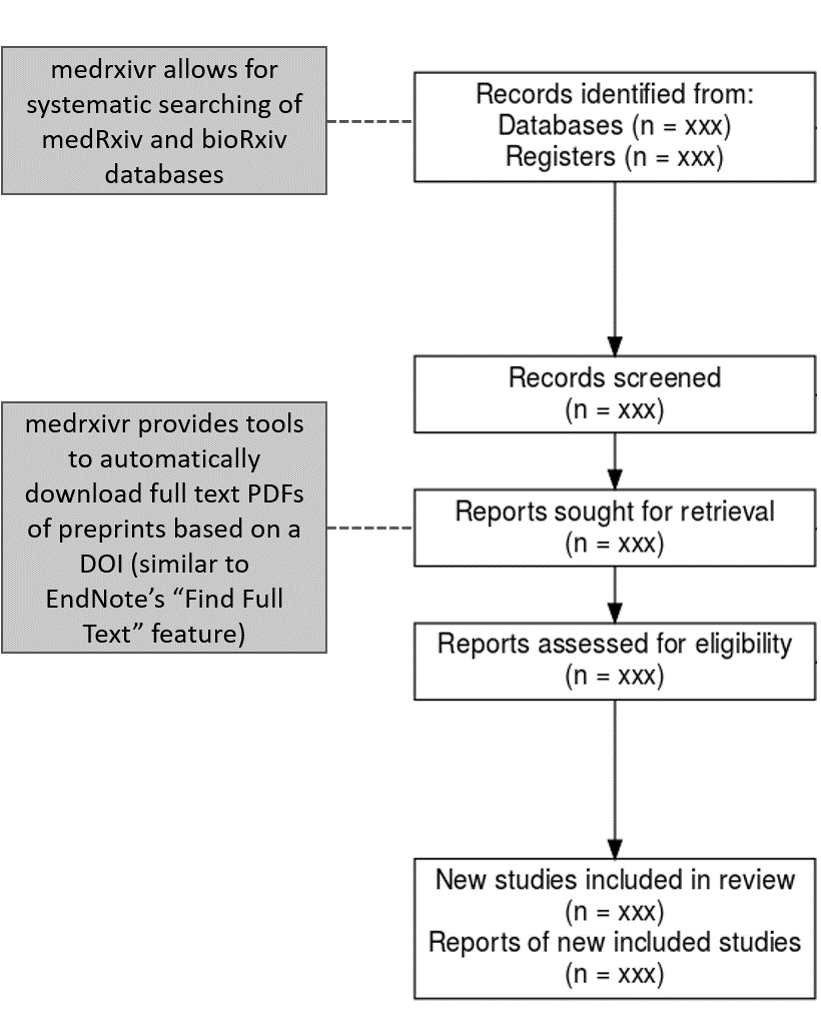
\includegraphics[width=0.65\linewidth]{figures/sys-rev-tools/medrxiv-role} 

}

\caption[Role of \texttt{medrxivr} in a systematic review workflow]{\textbf{Role of \texttt{medrxivr} in a systematic review workflow:} \texttt{medrxivr} allows for systematic searching of biomedical preprints as part of the initial literature searching. Following title and abstract screening, reviewers can then programmatically retrieve a copy of the PDF of included records to facilitate the full-text screening stage (similar to Endnote's ``Find Full Text'' feature).}\label{fig:medrxivr-sr}
\end{figure}

\hypertarget{development}{%
\section{Development}\label{development}}

\hypertarget{success-criteria}{%
\subsection{Success criteria}\label{success-criteria}}

The tool was developed to meet three success criteria,\textsuperscript{\protect\hyperlink{ref-wateridge1995}{120}} influenced both by the functionality required to perform systematic searches as part of the review in Chapter \ref{sys-rev-heading}, discussion with information specialist colleagues, and an informal survey of the evidence synthesis and health librarian communities on Twitter. The criteria were as follows:

\begin{enumerate}
\def\labelenumi{\arabic{enumi}.}
\item
  reliable, reproducible and transparent search functionality, allowing for Boolean (AND/OR/NOT) operator logic;
\item
  support for bulk export of references returned by the search to a file type that can be readily imported into a reference manager (e.g., \emph{.bib} or \emph{.ris}); and
\item
  automated retrieval of the full-text PDFs of relevant records, similar to the Find Full Text feature offered by EndNote.
\end{enumerate}

~

\hypertarget{alternative-medrxivbiorxiv-interfaces}{%
\subsection{Alternative medRxiv/bioRxiv interfaces}\label{alternative-medrxivbiorxiv-interfaces}}

Prior development of this tool, an audit of existing tools for accessing medRxiv and bioRxiv metadata was conducted. While none address the success criteria described above, two of these tools are useful to consider to highlight the additional functionality that \texttt{medrxivr} contributes.

The first, a platform called Rxivist,\textsuperscript{\protect\hyperlink{ref-abdill2019}{121}} allows users to search preprints using keywords. However, the core functionality of the Rxivist platform is focused around exploring the number of times a preprint has been downloaded and/or shared on Twitter, to allow researchers to find the most popular papers related to their topic. The search interface\footnote{Available at \url{https://rxivist.org/}} does not allow for complex search strategies using Boolean operators and there is no option to batch-export the results of a search.

The second tool, \texttt{search.bioPreprint}, allows users to search for terms across a range of preprint servers, including medRxiv and bioRxiv, but also journals which use a post-publication peer-review process such as F1000Research.\textsuperscript{\protect\hyperlink{ref-iwema2016}{122}} However, similar to the Rxivist platform, this tool is designed for researchers aiming to keep up to date with recent developments in their fields rather than systematically assess the entirety of the available literature. As such, the platform only returns the most recent 1,000 records by publication date.

Finally, neither tool provides an easy way to programmatically download a copy of the PDF of relevant preprints as part of the preparation for the full-text screening stage of a systematic review.

~

\hypertarget{early-versions}{%
\subsection{Early versions}\label{early-versions}}

Work on the \texttt{medrxivr} tool began in Summer 2019, and initially consisted of a development of set of R scripts to allow for searching medRxiv and bioRxiv as part of the systematic search outlined in Chapter \ref{sys-rev-heading}. Following interest from other researchers in using the \emph{ad-hoc} web-scraping scripts, additional development work took place in 2019/2020, allowing for improved searching and exporting functionality and the initial version of the \texttt{medrxivr} R package was released in February 2020.

Early versions of the tool had a reliance on scraping data directly from the repository website. Web-scraping is a fragile mechanism for extracting data, as it is entirely dependent on consistent website design and underlying code structure remaining unchanged.\textsuperscript{\protect\hyperlink{ref-shaw2002}{123},\protect\hyperlink{ref-laprie1992}{124}}. In the case of \texttt{medrxivr}, constant maintenance work was required to ensure the web-scraping script performed as expected, as the repository website was regularly updated.

However, an Application Programming Interface (API) for the medRxiv and bioRxiv repositories was made public in early 2020 by the institution responsible for managing these preprint repositories, the Cold Springs Harbor Laboratory. This allowed for newer versions of the \texttt{medrxivr} package to engage in active ``fault prevention'' and provide a more robust interface to the data by removing the reliance of web-scraping.\textsuperscript{\protect\hyperlink{ref-laprie1992}{124}}

~

\hypertarget{package-infrastructure}{%
\subsection{Package infrastructure}\label{package-infrastructure}}

The \texttt{medrxvir} package was written in R using RStudio,\textsuperscript{\protect\hyperlink{ref-rcoreteam2019}{125}} and followed development best-practice, including detailed documentation, a robust unit testing framework (99\% of all code lines within the package are formally tested across multiple platforms including Windows, MacOS, and Linux), and in-depth code review by two experienced, independent reviewers.

~

\hypertarget{usage}{%
\section{Usage}\label{usage}}

The \texttt{medrxivr} R package is split into two component parts:

\begin{itemize}
\tightlist
\item
  an interface to the Cold Springs Harbor Laboratory API, which imports medRxiv and bioRxiv metadata into R; and
\item
  a collection of functions for working with the imported metadata, with an explicit focus on searching this data as part of a systematic review or evidence synthesis project.
\end{itemize}

The standard workflow is to download a copy of all metadata contained in the repository, and then to perform searches on this local copy. This is a workaround as the Cold Springs Harbor Laboratory API does not provide any functionality to search the database.

While the package allows for users to search both medRxiv and bioRxiv, as the process is identical for both, the examples in the sections are limited to the medRxiv repository.

~

\hypertarget{installation}{%
\subsection{Installation}\label{installation}}

\texttt{medrxivr} has been released to the Comprehensive R Archive Network (CRAN), and can be installed with the following code:

~

\begin{Shaded}
\begin{Highlighting}[]
\FunctionTok{install.packages}\NormalTok{(}\StringTok{"medrxivr"}\NormalTok{)}
\end{Highlighting}
\end{Shaded}

~

Alternatively, the development version of the package can be installed from GitHub:

~

\begin{Shaded}
\begin{Highlighting}[]
\CommentTok{\# install.packages("devtools") }
\NormalTok{devtools}\SpecialCharTok{::}\FunctionTok{install\_github}\NormalTok{(}\StringTok{"ropensci/medrxivr"}\NormalTok{)}
\end{Highlighting}
\end{Shaded}

~

\hypertarget{importing-preprint-metadata}{%
\subsection{Importing preprint metadata}\label{importing-preprint-metadata}}

\texttt{medrixvr} provides two ways to access medRxiv data, as shown in Figure \ref{fig:medrxivr-data-sources}. The first, via the \texttt{mx\_api\_content()} function, creates a local copy of all data available from the medRxiv API at the time the function is run.

~

\begin{Shaded}
\begin{Highlighting}[]
\CommentTok{\# Get a copy of the database from the live medRxiv API endpoint}
\NormalTok{mx\_data }\OtherTok{\textless{}{-}} \FunctionTok{mx\_api\_content}\NormalTok{()  }
\end{Highlighting}
\end{Shaded}

~

The second, via the \texttt{mx\_snapshot()} function, provides access to a maintained static snapshot of the database, created each morning at 6am using \texttt{mx\_api\_content()}.

~

\begin{Shaded}
\begin{Highlighting}[]
\CommentTok{\# Import a copy of the medRxiv data from the snapshot}
\NormalTok{mx\_data }\OtherTok{\textless{}{-}} \FunctionTok{mx\_snapshot}\NormalTok{()}
\end{Highlighting}
\end{Shaded}

~

Allowing users of \texttt{medrxivr} to access a maintained snapshot removes any dependency on the API, which can become unavailable during peak usage times. The relationship between the two methods for accessing the data contained in the medRxiv database is summarized in Figure \ref{fig:medrxivr-data-sources}.

~





\begin{figure}[H]
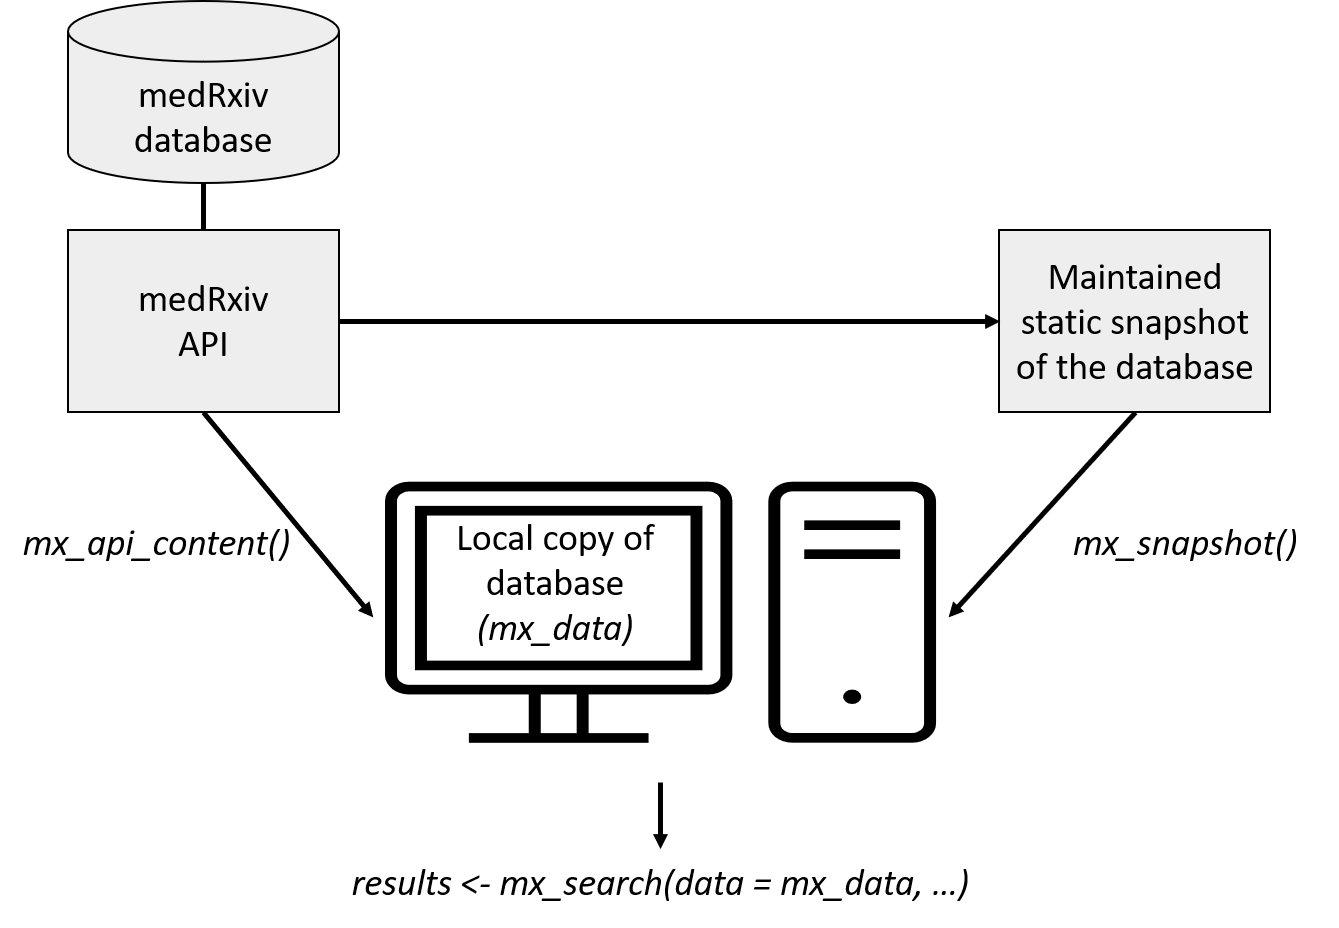
\includegraphics[width=1\linewidth]{figures/sys-rev-tools/data_sources} \caption[Overview of \texttt{medrxivr} data sources]{\textbf{Overview of \texttt{medrxivr} data sources:} Users can either access the API directly via \texttt{mx\_api\_content()}, or can import a maintained snapshot of the database, taken each morning at 6am, via the \texttt{mx\_snapshot()} function. Note: due to the size of bioRxiv, only a maintained snapshot of the medRxiv repository is available via \texttt{mx\_snapshot()}.}\label{fig:medrxivr-data-sources}
\end{figure}

~

~

\hypertarget{performing-a-search}{%
\subsection{Performing a search}\label{performing-a-search}}

Once a local copy of the metadata is created, the first step in searching it is to create a search strategy. Search terms to be combined with the OR operator are contained in vectors (\texttt{c(...)}), while topics to be combined with the AND operator are contained in lists (\texttt{list(\ldots{})}).

~

\begin{Shaded}
\begin{Highlighting}[]
\CommentTok{\# Create the search query}
\NormalTok{topic1  }\OtherTok{\textless{}{-}} \FunctionTok{c}\NormalTok{(}\StringTok{"dementia"}\NormalTok{,}\StringTok{"alzheimer\textquotesingle{}s"}\NormalTok{)  }\CommentTok{\# Combined with OR}
\NormalTok{topic2  }\OtherTok{\textless{}{-}} \FunctionTok{c}\NormalTok{(}\StringTok{"lipids"}\NormalTok{,}\StringTok{"statins"}\NormalTok{)        }\CommentTok{\# Combined with OR}

\NormalTok{myquery }\OtherTok{\textless{}{-}} \FunctionTok{list}\NormalTok{(topic1, topic2)         }\CommentTok{\# Combined with AND}
\end{Highlighting}
\end{Shaded}

~

For example, when written in standard syntax, the search contained in the \texttt{myquery} object above would be: ``((dementia \textbf{OR} alzheimer's) \textbf{AND} (lipids \textbf{OR} statins))''. There is no limit to the number of search terms that can be included in each topic, nor in the number of topics that can be search for. Search terms can also contain common syntax used by systematic reviewers and health librarians, including the use of NEAR statements which allows for identification of co-localised terms, and wild-cards, which allow for alternate spellings, e.g.~``randomi\emph{s}ation'' vs ``randomi\emph{z}ation''.

Once a strategy has been defined, it is passed along with the local copy of the database to the \texttt{mx\_search()} function.

~

\begin{Shaded}
\begin{Highlighting}[]
\CommentTok{\# Run the search}
\NormalTok{results }\OtherTok{\textless{}{-}} \FunctionTok{mx\_search}\NormalTok{(mx\_data,}
\NormalTok{                     myquery)}
\end{Highlighting}
\end{Shaded}

~

\hypertarget{refining-your-search}{%
\subsection{Refining your search}\label{refining-your-search}}

An important argument of the \texttt{mx\_search()} is \texttt{report}, which outputs a structured table with each search strategy presented on an individual line and the number of records associated with this strategy. \textbf{{[}CITATION NEEDED - PRISMA-S{]}}

~

\begin{Shaded}
\begin{Highlighting}[]
\NormalTok{results  }\OtherTok{\textless{}{-}} \FunctionTok{mx\_search}\NormalTok{(mx\_data,}
\NormalTok{                      myquery, }\CommentTok{\# Combined with OR}
                      \AttributeTok{report =} \ConstantTok{TRUE}\NormalTok{)}
\end{Highlighting}
\end{Shaded}

\begin{Shaded}
\begin{Highlighting}[]
\DocumentationTok{\#\# Found 1 record(s) matching your search.}
\DocumentationTok{\#\# }
\DocumentationTok{\#\# Total topic 1 records: 224}
\DocumentationTok{\#\# dementia: 224}
\DocumentationTok{\#\# alzheimer\textquotesingle{}s: 0}
\DocumentationTok{\#\# }
\DocumentationTok{\#\# Total topic 2 records: 119}
\DocumentationTok{\#\# lipids: 90}
\DocumentationTok{\#\# statins: 33}
\end{Highlighting}
\end{Shaded}

~

This allows users to discover which terms in their search are contributing most to the total number of results returned. This is important as part of developing a search strategy,\textsuperscript{\protect\hyperlink{ref-bramer2018}{126}} as it allows for the key terms related to each topic to be discovered. It also aids in identifying misspelled or case-sensitive search terms, which will frequently return no results. As an example, in the search presented above, the term ``alzheimer's'' returns no records. This is expected, as ``Alzheimer'' is a proper noun and so should be capitalised, but serves to illustrate the usefulness of the reporting function.

~

\hypertarget{exporting-to-a-bibliography-file}{%
\subsection{Exporting to a bibliography file}\label{exporting-to-a-bibliography-file}}

In line with the second success criteria (Section \ref{success-criteria}), one of the key features of the \texttt{medrxivr} is the ability for users to easily export the results of their systematic search to a reference manager. While it is a seemingly simple request, this is is one of the key ways in which \texttt{medrxivr} is set apart for other preprint search tools, including the native medRxiv/bioRxiv website search functionality.

For example, the results of our simple search above can be exported to the \texttt{"medrxiv\_export.bib"} file using the following code:

\begin{Shaded}
\begin{Highlighting}[]
\FunctionTok{mx\_export}\NormalTok{(results, }
          \AttributeTok{file =} \StringTok{"medrxiv\_export.bib"}\NormalTok{,}
          \AttributeTok{report =} \ConstantTok{TRUE}\NormalTok{)}
\end{Highlighting}
\end{Shaded}

~

\hypertarget{downloading-the-pdfs-of-relevant-records}{%
\subsection{Downloading the PDFs of relevant records}\label{downloading-the-pdfs-of-relevant-records}}

\texttt{medrxivr} alos allows users to download the full text papers for records that are deemed eligible for full-text screening (see Figure \ref{fig:medrxivr-sr}). \texttt{mx\_download()} takes the list of included records and saves the PDF for each to a folder specified by the user. This functionality is similar to the ``Find Full Text'' feature offered by EndNote.

~

\begin{Shaded}
\begin{Highlighting}[]
\FunctionTok{mx\_download}\NormalTok{(results,  }\CommentTok{\# Search results, less excluded records}
            \StringTok{"pdf/"}\NormalTok{)   }\CommentTok{\# Directory to save PDFs to }
\end{Highlighting}
\end{Shaded}

~

\hypertarget{discussion}{%
\section{Discussion}\label{discussion}}

\hypertarget{reception-and-future-plans}{%
\subsection{Reception and future plans}\label{reception-and-future-plans}}

The tool has been well received by the community (as of December 2021, \texttt{medrxivr} has been downloaded more than 4000 times), and several use cases have been reported. It has been used to investigate the role of preprints in the response to the 2019 coronavirus outbreak,\textsuperscript{\protect\hyperlink{ref-kodvanj2020}{127}} perform searches of preprints as part of a systematic review,\textsuperscript{\protect\hyperlink{ref-noone2020}{128},\protect\hyperlink{ref-grassly2020}{129}} and examine how data-sharing behaviour is affected by journal policies (see \ref{thesis-output}).\textsuperscript{\protect\hyperlink{ref-mcguinness2020c}{130}}

The package was been onboarded into the rOpenSci suite of packages, a collection of ``carefully vetted, staff- and community-contributed R software tools that lower barriers to working with scientific data sources on the web''.\textsuperscript{\protect\hyperlink{ref-boettiger2015}{131}} As part of this process, following rigorous peer-review, an associated article introducing the tool was published by the Journal of Open Source Software.\textsuperscript{\protect\hyperlink{ref-mcguinness2020a}{132}} The entire review discussion is publicly available and can be viewed online.\footnote{\url{https://github.com/ropensci/software-review/issues/380}} The tool has also been well received by the open-source community, demonstrated by the engagement of other developers in contributing to important new functionality and suggesting bug-fixes.

Lobbying of the Cold Springs Harbor Laboratory to develop the API to allow for direct searching of the database has been ongoing. This would negate the current need to download a local copy of the relevant preprint database before searching it, which is currently the rate limiting step for performing searches. For example, as of January 2021, downloading a copy of the bioRxiv database takes approximately an hour.

~

\hypertarget{limitations-of-medrxivr}{%
\subsection{\texorpdfstring{Limitations of \texttt{medrxivr}}{Limitations of medrxivr}}\label{limitations-of-medrxivr}}

While searching of the medRxiv and bioRxiv databases was crucial for the systematic review element of this thesis presented in Chapter \ref{sys-rev-heading}, there are some important limitations to note here. A key example is that the tool only searches the available metadata of preprint records (the title, abstract and keywords), rather than the full text of preprints, meaning some relevant records might be missed. However, this approach echoes that used by other search platforms such as OvidSP, and while some relevant records may be missed (reduced sensitivity), limiting the search to the metadata fields prevents non-relevant records from being returned (high specificity). A key example of the reduced specificity when searching the full text, identified during development of \texttt{medrxivr}, is that a search for ``dementia'' would return a record where the only occurrence of this term is in the title of one of the references.\textsuperscript{\protect\hyperlink{ref-bong2019}{133}}

There is also the potential that the cross-section of literature posted on medrxiv/bioRxiv is substantially different from the true grey literature (studies or analyses that are not published for a range of reasons including results that are not deemed ``novel'' or are not statistically significant).\textsuperscript{\protect\hyperlink{ref-song2010}{134}} This is because simply lowering the barriers to publication may well encourage authors to published ``null'' results, but due to the effort involved in writing up a distributable manuscript, it is unlikely to completely address the ``file drawer'' effect.\textsuperscript{\protect\hyperlink{ref-rosenthal1979}{86}} It is likely too early (and likely too methodologically difficult) to tell whether the increased popularity and acceptance of preprint repositories will have any effect of the availability of research that was not considered ``publishable'' at other venues.

~

\hypertarget{role-of-open-source-tools-in-evidence-synthesis}{%
\subsection{Role of open source tools in evidence synthesis}\label{role-of-open-source-tools-in-evidence-synthesis}}

Part of the motivation for creating the \texttt{medrxivr} tool was a belief that the development and distribution of open source scripts and tools should be a fundamental part of evidence synthesis research.\textsuperscript{\protect\hyperlink{ref-goldacre2019b}{135},\protect\hyperlink{ref-mckiernan2016c}{136}} In the case of \texttt{medrxivr}, it is likely that several other evidence synthesists had written personal scripts that have a similar, or related, functionality - in fact, following development of the tool, I identified one other researcher that has done so (Nicholas Fraser, author of the \texttt{rbiorxiv} package, which allows for importing medRxiv metadata into R but does not provide search functionality).\textsuperscript{\protect\hyperlink{ref-rbiorxiv}{137}} If these scripts continue to be developed in private and are never shared or publicised, this will inevitably harm to the evidence synthesis community, not only in terms of duplication of time and effort but also due to lost opportunities for collaboration.\textsuperscript{\protect\hyperlink{ref-mckiernan2016c}{136}} Creating and sharing well-documented packages, the recognised standard for sharing code in R, represents one way to reduce this inefficiency.\textsuperscript{\protect\hyperlink{ref-vuorre2020}{138}}

\hypertarget{summary-1}{%
\section{Summary}\label{summary-1}}

\begin{itemize}
\item
  In this Chapter, I have introduced a new tool, \texttt{medrxivr}, for performing complex systematic searches of the medRxiv and bioRxiv preprint repositories.
\item
  I have outlined the motivation for developing this tool in relation to this thesis - more specifically, that it was used to perform systematic and reproducible searches of a key literature sources used in the comprehensive systematic review described in Chapter \ref{sys-rev-heading}.
\item
  I have contrasted \texttt{medrxivr} with other available interfaces to medRxiv/bioRxiv data to highlight the added functionality it offers. I have also discussed the tools reception to date, its limitations, and the important role of open-source tools like \texttt{medrxivr} in evidence synthesis.
\end{itemize}

\newpage

\hypertarget{references-1}{%
\section{References}\label{references-1}}



\hypertarget{sys-rev-heading}{%
\chapter{Systematic review of all available evidence}\label{sys-rev-heading}}

\minitoc 

\hypertarget{lay-summary-2}{%
\section{Lay summary}\label{lay-summary-2}}

The importance of

I found that

The results of this review are used to guide the primary analysis presented in Chapter \ref{cprd-analysis-heading}, in addition to forming a key evidence source used in the triangulation exercise presented in Chapter \ref{discussion-heading}.

~

\hypertarget{sys-rev-intro}{%
\section{Introduction}\label{sys-rev-intro}}

The aim of this chapter is to systematically review all available literature on the association between blood levels of total cholesterol and it's constituent parts (HDL-c,LDL-c and triglycerides) on the subsequent risk of dementia.

Based on the review of existing literature, no previous evidence synthesis exercise attempted to examine all available literature simultaneously.

Only by looking across all available evidence can the true, given the often limited use of one type of evidence (RCTs are hard to do, obs studies are biased).

Literature con

Systematic reviews aim to transparently and reproducibly identift

~

\hypertarget{methods}{%
\section{Methods}\label{methods}}

\hypertarget{protocol}{%
\subsection{Protocol}\label{protocol}}

A pre-specified protocol for this analysis was registered using the Open Science Framework, and is available for inspection.\textsuperscript{\protect\hyperlink{ref-mcguinnessluke2020}{140}}

\hypertarget{search-strategy}{%
\subsection{Search strategy}\label{search-strategy}}

I systematically search electronic bibliographic databases to identify potentially relevant records. The search strategy used in each database was developed in an iterative manner using a combination of free text and controlled vocabulary (MeSH/EMTREE)\textsuperscript{\protect\hyperlink{ref-lefebvre2019searching}{82}} terms to identify studies which have examined the relationship between blood lipids levels and dementia, incorporating input from an information specialist. The strategy will include terms related to lipids, lipid modifying treatments, and dementia and its sub-types, and was designed for MEDLINE before being adapted for use in the other bibliography databases listed. An outline of the general strategy is presented in the Table \ref{tab:searchOverview-table} below and the full draft search strategies for each database are presented in Appendix \ref{appendix-search-strategy}.

~





\begin{table}[H]

\caption[searchOverview]{\label{tab:searchOverview-table}Summary of systematic search by topic. The full search strategy including all terms and the number of hits per term is included in Appendix \ref{appendix-search-strategy}.}
\centering
\fontsize{10}{12}\selectfont
\begin{threeparttable}
\begin{tabular}[t]{>{}cl}
\toprule
\textbf{No.} & \textbf{Concept}\\
\midrule
1 & Dementia/Mild Cognitive Impairment\\
\midrule
2 & Lipids\\
\midrule
3 & Lipid-modifying treatments\\
\midrule
4 & 1 AND 2\\
\midrule
5 & 1 AND 3\\
\midrule
\addlinespace
6 & 4 OR 5\\
\midrule
7 & Animals NOT (Animals AND Humans)\\
\midrule
8 & 6 NOT 7\\
\midrule
9 & Observational filter\\
\midrule
10 & Randomised controlled trial (RCT) filter\\
\midrule
\addlinespace
11 & Mendelian randomisation/Instrumental variable filter\\
\midrule
12 & OR/ 9-11\\
\midrule
13 & 8 AND 12\\
\bottomrule
\end{tabular}
\begin{tablenotes}
\item For all topics, search queries were comprised of relevant free text \& controlled vocabulary terms.
\end{tablenotes}
\end{threeparttable}
\end{table}

~

To ensure that the study design filters are not excluding potentially relevant records, a random sample of 500 records identified by the main search but excluded by the filters (defined as ``8 NOT 14'' in Table \ref{tab:searchOverview-table}) was screened. If any potentially relevant studies are identified, their titles and abstracts were searched for key terms that can be incorporated into the filters to improve search sensitivity.

The following databases were searched from inception onwards: Medline, EMBASE, Psychinfo, Cochrane Central Register of Controlled Trials (CENTRAL), and Web of Science Core Collection (for the specific databases available thi via the University). We will also search clinical trial registries, for example ClinicalTrials.gov, to identify relevant randomized controlled trials. As the contents of the Web of Science Core COllection can vary by institution, the specific database searched via this platform are listed in Appendix \ref{appendix-wos-databases}.

The abstracts list of relevant conferences (e.g.~the proceedings of the Alzheimer's Association International Conference, published in the journal Alzheimer's \& Dementia) were searched by hand.

Grey literature will also be searched via ProQuest, OpenGrey and Web of Science Conference Proceedings Citation Index, while theses were accessed using the Open Access Theses and Dissertations portal. We will also search bioRxiv and medRxiv, preprint repositories using a tool built as part of this thesis, to identify potentially relevant studies. Finally, the reference lists of included studies were searched by hand while studies citing included studies will be examined using Google Scholar (forward and reverse citation searching).

\hypertarget{study-selection}{%
\subsection{Study selection}\label{study-selection}}

Records were imported into Endnote and deduplicated using the method outlined in Bramer et al.~(2016).\textsuperscript{\protect\hyperlink{ref-bramer2016}{141}} In summary, this method uses multiple stages to identify potential duplicates, beginning with automatic deletion of records matching on multiple fields (``Author'' + ``Year'' + ``Title'' + ``Journal''), followed by manual review of less similar articles (e.g.~those matched based on the ``Title'' field alone).

Screening (both title/abstract and full-text) was performed using a combination of Endnote, a citation management tool,\textsuperscript{\protect\hyperlink{ref-hupe2019}{142}} and Rayyan, a web-based screening application.\textsuperscript{\protect\hyperlink{ref-ouzzani2016}{143}} Title and abstract screening to remove obviously irrelevant records was performed primarily by the primary author, with a random selection of excluded records being screened in duplicate to ensure consistency with the inclusion criteria.

Full-text screening will also be completed in full by the primary author. A second reviewer screened a random sample (approx 10\%) of included and excluded records, in addition to any records identified by the first reviewer as being difficult to assess against the inclusion criteria. Reasons for exclusion at this stage were recorded. Disagreements occurring during either stage of the screening process were resolved through discussion with a senior colleague. A PRIMSA flow diagram will be produced to document how records moved through the review.\textsuperscript{\protect\hyperlink{ref-zotero-766}{144}}

\hypertarget{inclusion-criteria}{%
\subsubsection{Inclusion criteria}\label{inclusion-criteria}}

We will seek studies that examine the relationship between blood lipid levels (or any specific lipid fraction, including total cholesterol, HDL, LDL, and triglycerides) and risk of incident dementia/MCI. Eligible study designs include randomized controlled trials and non-randomized observational studies of lipid modifying treatments, longitudinal studies examining the effect of increased/decreased blood lipid levels, and genetic instrumental variable (Mendelian randomization) studies examining the effect of genetically increased/decreased blood lipid levels.

Participants were free (or assumed to be free) of dementia/MCI at baseline. Studies of any duration were included to allow for exploration of the effect of length of follow-up on the effect estimate using meta-regression. No limits will be placed on the sample size of included studies.

Eligible studies defined dementia according to recognised criteria, for example the National Institute of Neurological Disorders and Stroke Association-Internationale pour la Recherche en l'Enseignement en Neurosciences (NINDS-AIREN), International Classification of Diseases (ICD), or Diagnostic and Statistical Manual of Mental Disorders (DSM) criteria.
For MCI, eligible studies are those that attempted state a definition for diagnoses of MCI (e.g.~an adapted version of the Petersen criteria)\textsuperscript{\protect\hyperlink{ref-petersen1999}{145}} and create ordinal groups of patients (e.g.~no dementia or dementia/MCI/dementia) based on this definition.

No limitations will be imposed on publication status, publication date, venue or language, although sufficiently detailed reports of the studies to be able to examine their methods were required for inclusion.

\hypertarget{exclusion-criteria}{%
\subsubsection{Exclusion criteria}\label{exclusion-criteria}}

Case-control studies, cross-sectional studies, qualitative studies, case reports/series and narrative reviews will be excluded. Studies which present no evidence of attempting to exclude prevalent cases from their analyses will also be excluded. Studies that measure change in continuous cognitive measures (e.g.~MoCA score) without attempt to map these scores to ordinal groups (e.g.~no dementia/MCI/dementia) will be excluded. Conference abstracts with no corresponding full-text publication will be examined, and we will contact authors to obtain information on the study's status. Studies that are reported in insufficient detail (e.g.~only in conference abstracts, new, letters, editorials and opinion) will be excluded. Previous systematic reviews will not be eligible, but their reference lists will be screened to identify any potentially relevant articles. Studies with outcomes not directly related to the clinical syndrome of dementia (e.g., neuroimaging), studies implementing a ``multi-domain intervention'' where the lipid-regulating agent is included in each arms (e.g.~for example, a study examining exercise + statins vs statins alone, but a study examining exercise + statins vs exercise alone would be included), and studies where there was no screening for dementia at baseline except if the sample was initially assessed in mid-life (i.e.~below the age of 50) will be excluded.

Excluded studies performing autopsy unless it was done under accepted criteria Exclude studies using a dietary intervention, for example omega-3 fatty acid enriched diet, as it hard to disentangle the effect of other elements contained within te diet, vs simple tablet based supplements of

~

\hypertarget{assessment-of-inter-rater-reliability}{%
\subsubsection{Assessment of inter-rater reliability}\label{assessment-of-inter-rater-reliability}}

Inter- and intra-rater reliability was assessed for a 10\% sub-sample of records at the title and abstract screening stage. Intra-rater reliability involved a single reviewer applying the inclusion criteria to the same set of records while blinded to their previous decisions, while inter-rater reliability involved two reviewers independently screening the same set of records.

If this approach demonstrates a significant level of erroneous exclusion by the primary author a larger proportion will be dual-screened.

Rater reliability was assessed using Gwet's agreement coefficient (AC1).\textsuperscript{\protect\hyperlink{ref-gwet2008}{146}} This measure of inter-rater reliability was chosen over other methods of assessing inter-rater reliability such as percent agreement (number of agreements divided by total number of assessments), as it accounts for chance agreement between reviewers but does not suffer from bias due to severely imbalanced marginal totals in the same way that Cohen's \(kappa\) value does.\textsuperscript{\protect\hyperlink{ref-gwet2008}{146}} Given the small number of included studies in this review, this is an important characteristic.

Gwet's AC1 is defined as:

\[AC1 = \frac{observed\;agreement-chance\;agreement}{1-chance\;agreement}\]

In reference to a two-by-two table with cells A, B, C and D, it is calculated using the following:

\[AC1 = \frac{\frac{A+D}{N}-e(\gamma)}{1-e(\gamma)}\]

where \(e(\gamma)\) is the chance agreement between raters, given as \(2q(1-q)\), where

\[q = \frac{(A+C)+(A+B)}{2N}\]

How to interpret agreement co-efficients is widely debated, and while arbitary cut-off values may mislead,\textsuperscript{\protect\hyperlink{ref-brennan1992}{149}} they provide a useful rubric by which to assess inter-rater agreement. Here, I used guidelines based on a stricter interpretation of the Cohen's \(kappa\) coefficient,\textsuperscript{\protect\hyperlink{ref-mchugh2012}{150}} presented in Table \ref{tab:gwet-table}.

~





\begin{table}[H]

\caption[Ranges for Gwet's AC1]{\label{tab:gwet-table}Suggested ranges to aid in interpretation of Gwet's AC1 inter-rater reliability metric}
\centering
\begin{tabular}[t]{cc}
\toprule
\textbf{Kappa} & \textbf{Interpretation}\\
\midrule
0    – 0.20 & None\\
\midrule
0.21 – 0.39 & Minimal\\
\midrule
0.40 – 0.59 & Weak\\
\midrule
0.60 – 0.79 & Moderate\\
\midrule
0.80 – 0.90 & Strong\\
\midrule
\addlinespace
> 0.90 & Almost perfect\\
\bottomrule
\end{tabular}
\end{table}

~

\hypertarget{data-extraction}{%
\subsection{Data extraction}\label{data-extraction}}

Harmonization of cholesterol measures across studies was performed, as different studies used different methods to quantify exposure, including comparing differing risks in the highest vs lowest quartiles of a lipid, using a binary classification of patients into a hypercholesterolaemia or not, categorizing lipid levels into high, middle, and low groups according to study-defined criteria, and simply treating the exposure as a continuous variable.

Following guidance for a dose response meta-analysis, I picked midpoint for all studies where bands were provided (extremely common in the case of lipids)

This analysis was unusual, as multiple methods of integration and analysis were required with data spanning many forms.

A piloted data extraction for was used. I extracted the data in the first instance and subset was checked by a colleague for accuracy.

Where necessary, lipid levels reported in \emph{mmol/L} were converted in \emph{mg/dL} using the following formula:

\begin{equation} 
  mg/dL = mmol/L \times{} Z
  \label{eq:lipidConversion}
\end{equation}

where \(Z = 38.67\) for total cholesterol, LDL-c and HDL-c, and \(Z = 88.57\) for triglycerides. For widely-used categorises of lipids levels on the \emph{mg/dL} scale, see Table \ref{tab:lipidLevels-table} in Section \ref{intro-lipid-fractions}.

\hypertarget{risk-of-bias}{%
\subsection{Risk of bias assessment}\label{risk-of-bias}}

A key use of the review presented in this chapter is to identify different sources of evidence at risk of a diverse range of biases, and to contrast and compare findings across them (see Section \ref{intro-triangulation} and Section \ref{triangulation-overview} for an overview of triangulation). To enable this triangulation exercise, a detailed and structured risk of bias assessment formed an important part of this review.

There has been a recent movement within the evidence synthesis community from examining \emph{methodological quality} to assessing \emph{risk of bias},\textsuperscript{\protect\hyperlink{ref-mcguinness2018a}{151},\protect\hyperlink{ref-sterne2016}{152}} and thus directly evaluating the internal validity of a study. Internal validity is defined here as the absence of systematic error (or bias) in a study, which may influence its results.\textsuperscript{\protect\hyperlink{ref-campbell1957}{153},\protect\hyperlink{ref-juni2001}{154}}

This move was prompted by a unclear definition of ``methodological quality'' which could include facets such as, and challenges in the comparison of results from different tools.

As part of this, the community also moved from checklist or score based tools towards domain-based methods, in which different potential sources of bias in a study are assessed in order.

Additionally, results should be assessed at the result (defined as a a specific outcome at a specific timepoint) rather than the study level. For example, a study may report on the efficacy of an intervention at 6 months and two years follow-up. missing outcome data that is not an issues at 6 months may introduce bias at 2 year follow-up. In this case, assigning a bias judgement to the study as a whole hides this differential biases for each result.

In this review, domain-based tools were used to assess the risk of bias for each result in each included study. The study design-specific tools are introduced and discussed in more detail in the following sections.

\hypertarget{randomised-controlled-trials-1}{%
\subsubsection{Randomised controlled trials}\label{randomised-controlled-trials-1}}

Risk of bias assessment in randomised controlled trials was performed using the domain-based risk-of-bias assessment tool appropriate to the study design. Randomized controlled trials were assessed using the RoB2 tool,\textsuperscript{\protect\hyperlink{ref-sterne2019}{155}},
The tool assess the risk of bias across five domains: Bias arising from the randomization process, Bias due to deviations from intended intervention, Bias due to missing outcome data, Bias in measurement of the outcome, Bias in selection of the reported result. Acceptable judgements include: low risk of bias, some concerns, high risk of bias. Each of the 5 domains contains a series of signalling questions or prompts, which guide the user through the tool.

One a domain-level judgement for each domain has been assigned, an overall judgement, using the same three levels of risk of bias, is assigned to

\hypertarget{non-randomised-studies-of-interventionsexposures}{%
\subsubsection{Non-randomised studies of interventions/exposures}\label{non-randomised-studies-of-interventionsexposures}}

For non-randomised studies of interventions (NRSI), I used the ROBINS-I (Risk of bias in non-randomised studies - of interventions) tool.\textsuperscript{\protect\hyperlink{ref-sterne2016}{152}} This tool assess the risk of bias across seven domains: Bias due to confounding, Bias due to selection of participants, Bias in classification of interventions, Bias due to deviations from intended interventions, Bias due to missing data, Bias in measurement of outcomes, and Bias in selection of the reported result. Similar to the RoB 2, it has a number of prompting questions per domain, with judgements including. Ideally, obs studies assessed in reference to an idealised randomised controlled trial. Further, the rare overall judgement of Low should be considered equivalent to a randomised controlled trial.

For non-randomised studies of exposures (NRSE), I opted to use a preliminary version of the ROBINS-E tool, despite it still being in development.\textsuperscript{\protect\hyperlink{ref-morganr2020}{156}} While the signalling questions for each domain are yet to be confirmed, the overarching domains have been finalised.

Despite these limitations, I chose this approach in place of other existing published tools such as the Newcastle-Ottowa scale (NOS).\textsuperscript{\protect\hyperlink{ref-wells2000newcastle}{157}} The motivation for this decision was two-fold. In the first instance, as mentioned in the introduction to this section, using a domain-based tool has distinct advantages over better-developed checklist-type tools such as the NOS. In addition, using a domain-based tool enabled better comparison with risk-of-bias assessments performed for the other study designs.

\hypertarget{mendelian-randomisation-studies}{%
\subsubsection{Mendelian randomisation studies}\label{mendelian-randomisation-studies}}

At present, no risk-of-bias assessment tool for Mendelian randomization studies is available. Assessment of the risk of bias in Mendelian randomisation studies was informed by the approach used in a previous systematic review of Mendelian randomisation,\textsuperscript{\protect\hyperlink{ref-mamluk2020}{158}} as identified by a review of risk of bias assessments in systematic reviews of MR studies. A copy of this tool is available in Appendix \ref{appendix-mr-rob}. Advance results from this review of bias assessment in MR studies were obtained from contact with the authors.

\hypertarget{risk-of-bias-due-to-missing-evidence}{%
\subsubsection{Risk of bias due to missing evidence}\label{risk-of-bias-due-to-missing-evidence}}

A recent shift towards the assessment of missing evidence due to selective non-reporting (as distinct from the selective reporting of a single result from multiple planned - handled in Domain 5 of the RoB 2 tool for example).

As part of this review, I piloted the RoB-ME (Risk of Bias due to Missing Evidence in a synthesis) tool. Results were visualise

\hypertarget{studification}{%
\subsection{Studification}\label{studification}}

Multiple publications resulting from the analysis of the same data were included and grouped ().

In the advent of multiple papers reporting results on the same cohort, but say, at different time points, I used a process of studifiction to build out the most comprehensive accounts of the studies and results from as many published articles were applicable.

This was particularly relevant to preprints and published papers reporting the same study, which were not considered duplicate records. Instead, they were considered as different reports of the same study. This is due to the potential for the published version to offer some information that the preprint did not, and vice versa.

\hypertarget{contacting-authors}{%
\subsection{Following up with authors}\label{contacting-authors}}

Where data points required either for the analysis or risk-of-bias assessment but were not reported, the primary authors of the study were contacted. This approach was taken due to the potentially large impact of following up with authors on the results of the review,\textsuperscript{\protect\hyperlink{ref-reynders2019}{159}}

This was particular important for the dose response meta-analysis, we

Use the example of getting the cut-off points from the

\hypertarget{analysis-methods}{%
\subsection{Analysis methods}\label{analysis-methods}}

\hypertarget{standard-meta-analysis}{%
\subsubsection{Standard meta-analysis}\label{standard-meta-analysis}}

Meta-analysis is an important method of . . .

Both a fixed-effect and random-effects meta-analysis model was.

For

Need formula here, and description of different methods and quarrels regarding disctinction fixed effect vs random effects meta-analyses.

This analytical approach was used for

\hypertarget{dose-response-analyses}{%
\subsubsection{Dose-response analyses}\label{dose-response-analyses}}

Several of the included studies presented data on multiple categories of lipid levels, but provided an overall effect estimate based on a comparison of only two of these categories (e.g.~for example, highest vs lowest quartile).
while this allows for easy interpretation of the resulting effect estimate, it ignores any potential non-linear relationships between the exposure and outcome, in addition to discarding useful information contain in the interim groups.

Where possible, data for all exposure groups was extracted, and this
. Studies were excluded from this analysis if the number of categories was less than three, if the exposure cut-off points for for each category were not presented (e.g.~if the study reports splitting participants into quartiles and comparing the highest vs lowest without giving the quartile bands in mmol/L).

A XXXX spline model was fitted to allow for a non-linear relationship, for example a U or J-shaped relationship, where low and high levels of an exposure can have an effect versus the ``normal'' reference dose. Reference doses were defined \emph{a priori} as the cut-off of the ``Normal''/``Optimal'' categories for each fractions, as detailed in Table \ref{tab:lipidLevels-table}. Under this approach, the reference dose was defined as 200 mg/dL for total cholesterol, 100 mg/dL for LDL-c, 40 mg/dL for HDL-c, and 150 mg/dL for triglycerides.

Due to the requirements for the dose response analysis, studies were excluded from this secondary analysis if they did not provide the require information: cut-off points. Where this was not reported in the study, I contacted the corresponding author to attempt to obtain the required information (see \ref{contacting-authors}).

When the highest category was open ended (e.g LDL-c \(\geqslant\) 200 mg/dL), I calculated category midpoint by assuming the widht of the higest category was the same as the one immediately below it. Similarly, when, the lowest category was open-ended (e.g LDL-c \(\leqslant\) 100 mg/dL), I set the lower boundary for this category to zero (though this is unlikely to occur natually, it was difficult to define).

I assumed the width of the category to be the same as the adjacent category.
When the lowest category was open ended, I set the lower boundary to zero.

\hypertarget{sensitivity-analyses}{%
\subsubsection{Sensitivity analyses}\label{sensitivity-analyses}}

I conducted a leave one out analysis in order to explore the impact of any given study on the results.

In addition,

~

\hypertarget{visualisation-of-results}{%
\subsection{Visualisation of results}\label{visualisation-of-results}}

Given the importance of visualising the potential biases alongside the results of any given study, a new visualisation tool was designed to allow for ``paired'' forest plots (as recommended by the ROB2 publication)

This tool grew out of a collaboration with other reserachers to design a modular method for creating these plots

A summary of this tool is contained in Appendix \ref{appendix-robvis}, and all forest plots presented in this analysis were created using

Results from the risk-of-bias assessment were visualized using a paired forest/risk-of-bias blobbogram, created using the \texttt{robvis} tool. This tool was developed as an adjunct to this thesis to aid in creating standard risk-of-bias figures.\textsuperscript{\protect\hyperlink{ref-mcguinness2019}{160}} A summary of the tool is provided in Appendix \ref{appendix-robvis}.

~

\hypertarget{assessment-of-added-value-of-including-preprint}{%
\subsection{Assessment of added value of including preprint}\label{assessment-of-added-value-of-including-preprint}}

Preprints are a valuable evidence source (see Introduction) but their inclusion in a systematic reivew
s
Additionally, I followed preprints up over time to investigate whether all identified preprints included in the review were subsequently published (in which case preprints give you a look into the future, and a systematic review update would capture these reports) or alternatively, if some preprints were not published, then preprints provide a different.

I also sought to explore the additional evidental value of including preprints in the meta-analysis, assessed using the fixed effect weight from a standard meta-analysis.

\hypertarget{patient-and-public-involvement}{%
\subsection{Patient and public involvement}\label{patient-and-public-involvement}}

Patient and

\hypertarget{deviations-from-the-protocol}{%
\subsection{Deviations from the protocol}\label{deviations-from-the-protocol}}

A dose response meta-analysis was not planned, marking a departure from the registered protocol.

\hypertarget{results}{%
\section{Results}\label{results}}

\hypertarget{search-and-screening-results}{%
\subsection{Search and screening results}\label{search-and-screening-results}}

Twenty-three thousand, four hundred forty-seven records were identified through database searches. Following depulication, 16,109 unique records remained.

\blandscape{}

~





\begin{figure}[H]

\includegraphics[width=1\linewidth]{figures/sys-rev/prismaflow} \caption[PRISMA flow diagram]{PRISMA Flow diagram illustrating how records moved through the systematic review process. The different contributions of databases and preprint servers to the review are indicated.}\label{fig:prisma-flow-fig}
\end{figure}

\elandscape{}

Following de-duplication, the titles and abstracts of 16,109 records were assessed for eligibility. 387 were deemed potentially eligible and the full text records for these were requested and screened. \ref{fig:prisma-flow-fig}

A PRISMA (Preferred Reporting Items for Systematic Reviews and Meta-analyses) flow diagram,\textsuperscript{\protect\hyperlink{ref-page2021}{161}} shown in Figure \ref{prisma-flow-fig}, illustrates the movement of articles through the review. To highlight the contribution of preprint archives to the review, the flow diagram delineates between those records captured through databases searches (presented on the right of the diagram) and those captured by the search tool described in the previous chapter (presented in grey on the left of the diagram).

Following screening, XXX studies were included.

The distribution of included studies over time demonstrates that despite the conduct of several previous reviews of different types of literature surrounding this question, primary studies continue to the published as these reviews have yet to provide a definite answer.

Table \ref{tab:incl-studies-character} shows the characteristics {[}\textbf{Include column here that says whether it was included in a systematic review - see below}{]}

As part of our our forward snowballing exercise (where articles citing an included study are cited), Irecorded whether a study included in our review had been included in any previous evidence synthesis attempt in an attempt to qualify the added value of this analysis. Additionally, if an included article was subsequently cited by a review, all studies in that review were screened for inclusion for the sake of completeness. This analysis was performed by extracting the citing articles from Google Scholar on {[}DATE{]} and screening them manually. The DOI of articles extracted from this analysis are included in the appendix, as the Google Scholar search functionality is not readily reproducible.*

As a summary of the duplication of work in this area, Ilooked at how many reviews a single included study had previously been included in.

~





\begin{table}[H]

\caption[Inter-rater agreement]{\label{tab:agreeInter-table}Inter-rater agreement on a subset of \textasciitilde10\% of records, illustrating high accuracy.}
\centering
\begin{tabular}[t]{>{}l>{}lr>{}r|r}
\toprule
\multicolumn{2}{c}{ } & \multicolumn{3}{c}{Initial screening decision} \\
\cmidrule(l{3pt}r{3pt}){3-5}
\textbf{} & \textbf{} & \textbf{Exclude} & \textbf{Include} & \textbf{Total}\\
\midrule
 & \textbf{Exclude} & 1244 & 9 & 1253\\
\cmidrule{2-5}
 & \textbf{Include} & 26 & 22 & 48\\
\cmidrule{2-5}
\multirow{-3}{*}{\raggedright\arraybackslash \textbf{Second reviewer decision}} & \textbf{Total} & 1270 & 31 & 1301\\
\bottomrule
\end{tabular}
\end{table}





\begin{table}[H]

\caption[Inter-rater agreement]{\label{tab:agreeIntra-table}Intra-rater agreement on subset of records, indicating high consistency.}
\centering
\begin{tabular}[t]{>{}l>{}lr>{}r|r}
\toprule
\multicolumn{2}{c}{ } & \multicolumn{3}{c}{Initial screening decision} \\
\cmidrule(l{3pt}r{3pt}){3-5}
\textbf{} & \textbf{} & \textbf{Exclude} & \textbf{Include} & \textbf{Total}\\
\midrule
 & \textbf{Exclude} & 1266 & 14 & 1280\\
\cmidrule{2-5}
 & \textbf{Include} & 4 & 17 & 21\\
\cmidrule{2-5}
\multirow{-3}{*}{\raggedright\arraybackslash \textbf{Same reviewer decision}} & \textbf{Total} & 1270 & 31 & 1301\\
\bottomrule
\end{tabular}
\end{table}

~

For the inter-rater reliability, agreement was very high (\(AC1\) = 0.97, \(kappa\) = 0.54, Table \ref{tab:agreeInter-table}). Agreement was similary high for intra-rater reliability (\(AC1\) = 0.99, \(kappa\) = 0.65, Table \ref{tab:agreeIntra-table}). The discrepancy between the \(AC1\) and \(kappa\) coefficients illustrates the sensitivity of \(kappa\) to imbalanced marginals, caused in this sample by a heavy imbalance towards exclusion.\textsuperscript{\protect\hyperlink{ref-feinstein1990}{162}}

Those records which were excluded in the initial screening, but were included by the second reviewer (n=26) were investigated. This discrepancy between the two reviewers was explained in all cases by differing interpretations of the inclusion criteria, specifically around the definition of cognitive decline versus mild cognitive impairment, and the definition of eligible lipids fractions.

Additionally, records I excluded on my second viewing (n=4) were investigated. All were . . .

\hypertarget{characteristics-of-included-studies}{%
\subsection{Characteristics of included studies}\label{characteristics-of-included-studies}}

XXXX studies met the criteria for inclusion in the review.

As shown in

Include here:

\begin{itemize}
\item
  PRISMA Flowchart
\item
  Summary of types of study
\item
  Summary of locations (use evidence map)
\item
  Summary of diagnostic criteria used
\item
  Summary of risk of bias
\item
  Long table, horizontally.
\end{itemize}

A common theme across the studies was a lack of data on vascular dementia. This is particularly interesting as lipids and statins are primarily a vascular disease. There is the potential that they studies encountered similar difficulties in address the unexpected results observed in the CPRD analysis in Chapter \ref{cprd-analysis-heading}. For vascular dementia, few studies exmined this outcome, primarily because of the absence (until recently) of

One item of particular interest in the absence of studies examining Mendelian randomisation studies is the absence of any effect following the adjustment for Apoe4. As covered in the discussion, ApoE4 genotype is the mjor risk factor for Alzheimer's disease.

In addition, there was quite a spread in terms fo the effect estimates used to th. Previous systematic review

\hypertarget{converting-risk-ratios-to-odds-ratios}{%
\subsection{Converting risk ratios to odds ratios}\label{converting-risk-ratios-to-odds-ratios}}

Include formulae and informed assumptions

\hypertarget{hazard-ratios-vs-riskodds-ratios}{%
\subsection{Hazard ratios vs risk/odds ratios}\label{hazard-ratios-vs-riskodds-ratios}}

Not interchangeable in the context of systematic review. If outcome is rare, odds and risk ratios approximate each other, but the hazard ratio is measuring something completely different, by taking into account time-to-event in each treatment group.

Several existing reviews do not distinguish between the two types of effect measures and include all existing studies in a single meta-analysis to produce an overall effect.

The likely effect of this is that the overall effect measures are biased towards . . . . ?

Can you predict the direction of effect from a

Best practice methods for dealing with disparate effect measures in included studies is to not perform a meta-analysis

Some evidence of manipulation of effect estimates in previous reviews,(e.g.~Chou, Sci Reports - at least one study disagrees with) but not documented in review text.

\hypertarget{risk-of-bias-subheading}{%
\subsection{Risk of bias}\label{risk-of-bias-subheading}}

\hypertarget{dose-response-meta-analysis}{%
\subsection{Dose response meta-analysis}\label{dose-response-meta-analysis}}

Several studies were excluded from the dose-response meta-analysis, as the number of cases/controls be

\hypertarget{sources-of-heterogeneity}{%
\subsection{Sources of heterogeneity}\label{sources-of-heterogeneity}}

Detail that some of these are exploratory, in particular the effect of different scales on the association between the groups. \textbf{{[}CROSS{]}}

\hypertarget{sys-rev-pub-bias}{%
\subsection{Publication bias}\label{sys-rev-pub-bias}}

\begin{itemize}
\tightlist
\item
  Check if there are protocols available for any of the published reports (unlikely for non-randomised controlled trials), and whether there were
\item
  Vascular dementia has substantially less published reports. Many (reference Smeeth et al 2010 here) simply group into AD and non-AD making comparison between published studies difficult
\end{itemize}

One particularly interesting meta-bias potentially applicable in this review is the definition of code lists across

Many studies did not report the codelists used to run the analysis,

\hypertarget{triangualtion-across-evidence-sources}{%
\subsection{Triangualtion across evidence sources}\label{triangualtion-across-evidence-sources}}

One key question for which multiple distinct sources of evidence were available were those looking at Laz

A key limitation for other types of dementia, in particularly vascular, is that there has yet to be a GWAS identifying relevant SNPS that could then be used in a MR study with SNPS for lipids to estimates the causal effect of lipids on vascular dementia {[}\textbf{Is this true?}{]} This rules out the use. In addition, there was limited literature available - as discussed in CHapter \ref{sys-rev}

Consideration of the potential impact of the magnitude and direct of residual confounders/bias is not a major stretch from what is already happening in the assessment of the quality of evidence (GRADE) framework. Within GRADE, the overall quality of evidence can be upgraded when there is deemed to be unmeasured or residual confounding variables which reduce the. For example, if the propensity to treatment is related to comorbidity burden, but those on treatment still have better outcomes then those on control, it is likely that the true effect of the intervention is being underestimated.\textsuperscript{\protect\hyperlink{ref-guyatt2011}{163}}

Without our framework and as part of the risk of bias assessments reported in \ref{risk-of-bias-subheading}, Itest test

\hypertarget{added-evidental-value-of-including-preprints-sys-rev-including-preprints}{%
\subsection{Added evidental value of including preprints \{sys-rev-including-preprints\}}\label{added-evidental-value-of-including-preprints-sys-rev-including-preprints}}

There were several relevant preprints captured by the search run using the tool presented in Chapter \ref{sys-rev-tools-heading} (see Appendix \ref{appendix-medrxivr-code}). While many of the preprints included were subsequently published by the time of submission of this thesis, at the time of the search they were only available

Good example is \url{https://doi.org/10.1101/168674}, which was subsequently published in Nature Comms but in 2020, following peer-review (found no impact of LDL-c on AD following removal of APOE4).

Of interest,

This likely reflects a bias in the type of study that is submitted, but indicates the additional evidential value of include preprints in the search strategy. It also means that searches are current - if the aim of systematic reviews is to

While the total number of relevant studies found using this method was

On further investigation, the argument that .

It is not so much that they provide a source of unpublished grey-literature, more so that they provide a ``future'' look at .

However, if the aim is to find the current state of the art in the topic area at the time of searching, inclusion of preprints is a requirement.

While concerns have been raised that

Previous meta-studies have found high concordance between the main interpretations and other study design details in preprint-journal article pairs,\textsuperscript{\protect\hyperlink{ref-shi2021}{164}} though quality of reporting was slightly better in formally published articles.\textsuperscript{\protect\hyperlink{ref-carneiro2020}{165}}

A common criticism of preprinted articles is that they have not formally been peer-reviewed. \textbf{{[}CITATION NEEDED{]}} However, I believe this criticism is less warranted in the context of inclusion of preprints in a systematic review, given a formal assessment of risk of bias, which provides a structured approach to assessing the internal validity of a study.

\begin{quote}
Anyone who can't assess a study to the level of peer review shouldn't do a systematic review
\end{quote}

References included in the review were also searched for on PubPeer, a platform which enables post-publication peer review of published journal articles.\textsuperscript{\protect\hyperlink{ref-hunter2012}{166}}

The added value of peer-review to papers that is questionable and difficult to quantify for a number of reasons, including the fact that most peer reviews are closed

While {[}\textbf{some}{]} preprint have subsequently been published, this does not cause any major issues.

\hypertarget{discussion-1}{%
\section{Discussion}\label{discussion-1}}

Major limitation is that several included studies used data from electronic health databases, which come with serious concerns regarding validity\textsuperscript{\protect\hyperlink{ref-hsieh2019}{167}} \textsuperscript{\protect\hyperlink{ref-mcguinness2019d}{168},\protect\hyperlink{ref-wilkinson2018b}{169}}

In addition, the a

\hypertarget{previous-reviews}{%
\subsection{Previous reviews}\label{previous-reviews}}

\textbf{Will need to include something in the methods section on this}

As part of this analysis, Iexamined the overlap between different published reviews on this topic.

Several primary studies were captured in multiple systematic reviews. However, some studies were not captured by any previous review,

An upset plot shows the total size of each set (in this case, the set of included studies in each review) in the bottom left hand bar plot. For example, the XXXX review includes XXXX studies.

Where a line joins two points in the matrix, the main barchart shows the number of records shared by these reviews. So for example, XXXX records were captured both by the XXXX review and the XXXX review.

Where the matrix has just a single point highlighted, this shows the records unique to that review.

The reviews are ordered by date, to attempt to show the increasing overlap and total number of studies

Our review is presented as the last point on this plot, and captured XXXX records

The alternative is to have a barplot showing the total cumulative number of records over the years, using our set as the master, with the bars coloured by the number of records included in 1/2/3/4 reviews. The information below the bar axis could then show the number of reviews published in that year, or alternative, you could have an upsidedown bar to show cumulative number of reviews on this topic.

Of note, this review did not include the commonly cited PROSPER study, which examined the effect of pravastatin on CVD risk and putatively provides no evidence for an effect of the statin on dementia outcomes. While widely cited and included in the Cochrane review on this topic, it has not been included here, for the reason that it only reported the change from cognitive score (as measured using the {[}CHECK{]} scale) over a mean follow-up. While this is a useful indicator of general cognitive decline, it is not equivalent to a dementia outcome, as cogntive scales should feed into a broader diagnostic pathway - See section \ref{diagnostic-criteria}

This does introduce some conflicts with other studies where a change score has been dichotomised in order to have a binary dementia or not dementia outcome.

Does it also cause issues in terms of self-report?

\hypertarget{comments-on-the-process}{%
\subsection{Comments on the process}\label{comments-on-the-process}}

As part of the reflective element of this thesis, I collated my experiences on performing a systematic review.

Systematic reviews should not be performed as part of a thesis, without suitable support and resourcing guaranteed. Assumption that everyone does a systematic review (without risk of bias assessments, inclusion of all literature, searching for other reviews) is foolish.

Average time to complete a s

However, new developments such as automated screening would allow for a reduced need for personnel to work on these things.

Great learning experience in terms of managing a team, but due to a rotating schedule of people, much harder to do that expected.

A final point on the progress of the review is that, due to the need for dual screening and data extraction, a number of external researchers became involved in this review. I found the people-management aspect particularly challenging and could definitely have improved the process through better communication of deadlines, but it has provided good experience of leading a review team.

\hypertarget{inclusion-of-preprints}{%
\subsection{Inclusion of preprints}\label{inclusion-of-preprints}}

As highlighted in Section \ref{diverse-sources-preprints}, this thesis explicitly sought to synthesize evidence across different publication statuses, predominantly preprinted vs published. Using the tool described in Chapter \ref{sys-rev-tools-intro}, two preprint serves related to health and biomedical sciences were search as part of this review.

The added evidential value of including these preprints was highlighted in Section \ref()

On further investigation, X of these preprints were subsequently published since the search was performed in 2019. While this provides some additional evidence that the quality of the research described by included preprints was sufficiently high to pass peer-review, it does not invalidate the approach, as the future publication status was unavailable at the time the search was conducted.

\hypertarget{sys-rev-open-data}{%
\subsection{Open data sharing}\label{sys-rev-open-data}}

As evidenced by the issues involved in obtaining

Building in part on the research, I co-wrote an guidance piece for pre

Similarly, a substanital amount of time and effort has gone into making the data obtained by this review openly available to

\hypertarget{original-contribution-to-research}{%
\subsection{Original contribution to research}\label{original-contribution-to-research}}

I believe there are four aspects where this review is distinct from those reviews already available in the published literature (as identified by ):

\begin{itemize}
\item
  \emph{Comprehensiveness:} While several reviews of this research topic exist,\textsuperscript{\protect\hyperlink{ref-chu2018b}{63},\protect\hyperlink{ref-yang2020}{170}--\protect\hyperlink{ref-poly2020b}{172}} the overlap between the list of studies included in each is not 100\%. As part of this review, I have not only performed a original search of primary literature databases, but have also screened the reference lists of comparable reviews to ensure no study has been omitted.
\item
  \emph{Structured risk of bias assessment:} The majority of the highly cited reviews on this topic either do not formally consider the risk of bias in the observational studies they include or do not use an appropriate domain-based assessment tool (e.g.~ROBINS-I/E). This is important area in which this thesis can add value, as based on the risk-of-bias assessments I have performed to date, several primary studies are at high risk of bias and this should be reflected in the findings of any review on this topic.
\item
  \emph{Inclusion of preprints:} Unlike other available reviews and enabled by the tool described in Chapter 3, this review systematically searched preprinted health-related manuscripts as a source of grey literature. As part of this chapter, I plan to examine the extent of the additional information provided to the review by the inclusion of preprints.
\item
  \emph{Contribution to methods work:} A large part of this review was the associated work on improving research synthesis methods. This work is detailed as relevant throughout the Chapter, often referring to additional work detailed in the . IN addition this review was used to pilot an upcoming risk of bias tool
\end{itemize}

\hypertarget{comparison-with-other-reviews}{%
\subsection{Comparison with other reviews}\label{comparison-with-other-reviews}}

Of note, as part of the review, Iidentified several previous systematic reviews of this topic.{[}CITE{]} However, this review is the first to use established domain based assessments tools (for example, the RoB 2 tool for randomized controlled trials)\textsuperscript{\protect\hyperlink{ref-sterne2019}{155}} to assess the risk of bias in included studies, and explore the heterogeneity of results across different levels of risk of bias levels.

Some previous reviews did assess risk of bias, but used non-domain based assessment tools. Newcastle-Ottowa scale,

\textbf{The duplication of work across reviews (including, ironically, by this review) is substantial. In Section XXXX, I demonstrated that the each primary study included in this review was also included in other review so this topic, but that not all studies were included in all reviews. However, by creating a comprehensive review that attempted to draw together all available evidence from across the full range of study types.}

\textbf{Exclusion of the PROSPER trial} Will need to have a good bit here on the exclusion of this RCT, particularly as it is included in the Cochrane review on the topic. Cross-reference with the meta-bias section in the early section, on the impact of only included studies that sought to make a definitive diagnosis, rather than using change in cognitive assessment scales.

\hypertarget{reviewing-mendelian-randomisations-studies}{%
\subsection{Reviewing Mendelian randomisations studies}\label{reviewing-mendelian-randomisations-studies}}

While

This may be because Mendelian randomisation studies have yet to reach a critical mass in terms of requiring a systematic review.

Recent updates, such as a guide to reading and interpreting Mendelian .

However, this guide includes reporting items in their quality checklist - reporting quality while important, is unrelated to internal validity.

Problems with overlapping samples in reviews of Mendelian randomisation studies in that may be double counting participants

Double-counting of other -

Methods for reviews of Mendelian randomisation studies are not well developed to account for the consideration above.

In short, given the recent developments in the production of studies and results from Mendelian randomisation

This is particularly relevant to missing evidence, as new methods in MR studies allow for the anlysis of many exposures/outcomes concurrently. In this scenario, missing evidence is likely to be an issue as onyl those of particular interest to the authors/those reaching statistical significance will be reported in the paper

This is highlighted by the identification of studies relevant to the review though coincidental reading and citation searhcing, that were not identified by the search as they reported many results and only the statistically significant ones were included in searchable fields

This is particularly troubling given the comprehensiveness of the search (\textasciitilde17,000 records screened). In retrospect, a mitigating approach may have been to have an additional search for topics related to risk factors, dementia and MR studies, and screened t

As a form of analysis that lends itself to multiple comparison, there is a strong

Through snowballing and other measures, I identified at least one Mendelian randomisation study that had not been identified by the search strategy.\textsuperscript{\protect\hyperlink{ref-larsson2017b}{173}} On review of this paper, the search would not have been expected to find it, given the absence of any lipid-related keywords in the title and abstract.

The study examined the association between lipid fractions with Azlheimer's disease, as one of many risk factors for AzD. Studies such as this can introduce bias, as it is commonly only those risk factors that show a statistically significant result that are reported in the abstract and so are captured by systematic reviews of the topic. This may bias reviews as the analysising multiple risk factors at a time becomes more common.

These studies are described as ``unknown unknown's'' in the context of the RoB-ME tool, and are particularly challenging (as opposed to an analysis that was insufficiently reported to be included in the statistical analysis, or the ``known unknown's''),

Is it a big issue that the studies have the same underlying datasets?

Potentially the use of methods such as snowballing (forwards and backwards citation chasing) and communication with relevant topic experts should cpature similar studies.
However, in future better-resourced reviews, a dedicated search for ``risk factors'' and ``dementia'' and ``Mendelian randomisation'', followed by manual review of studies that look across multiple risk factors, would be advisable.

\hypertarget{strenghts-and-limitations}{%
\subsection{Strenghts and limitations}\label{strenghts-and-limitations}}

\hypertarget{inclusion-of-mendelian-randomisation-studies}{%
\subsubsection{Inclusion of Mendelian randomisation studies}\label{inclusion-of-mendelian-randomisation-studies}}

\hypertarget{inclusion-of-preprints-1}{%
\subsubsection{Inclusion of preprints}\label{inclusion-of-preprints-1}}

Comment on the fact that several of the studies identified through the search of preprints, were subsequently published, but much later than the
cut-off point for the search (e.g.~they would not have been captured by the search for published papers)

\hypertarget{use-in-other-chapters}{%
\subsection{Use in other chapters}\label{use-in-other-chapters}}

Findings from this review are used though out the subsequent chapters.

For example,

\hypertarget{references-2}{%
\section{References}\label{references-2}}



\hypertarget{cprd-analysis-heading}{%
\chapter{Primary analysis of lipid regulating agents and dementia outcomes}\label{cprd-analysis-heading}}

\minitoc 

\hypertarget{lay-summary-3}{%
\section{Lay summary}\label{lay-summary-3}}

Electronic health record (EHR) databases are large collections of patients data, used to manage patient administration and care. Under these systems, whenever a patient attends their GP, their clinical data is recorded in a central database using a standard set of codes. These databases have several advantages over traditional methods of data collection, including the number of people they contain and the length of time for which participants are followed. This is particularly important when studying diseases such as dementia, which may begin to develop in patients long before symptoms are seen.

This analysis makes use of the Clinical Practice Research Datalink (CPRD), which contains the electronic medical records of more than 3 million people from general practices across the UK. Using this data, the analysis presented in this chapter examined the effect of treatment which lower cholesterol levels, such as statins, on the risk of dementia and related outcomes.

No evidence for an effect of lipid regulating agents effect on the risk of Alzheimer's disease was found, with the exception of a slightly increased risk in those prescribed a certain type of drugs called fibrates. In contrast, I found an increased risk of vascular and other (i.e.~non-Alzheimer's) dementia with lipid regulating agent use.

This increased risk is unexpected, and is very likely to be due to the presence of bias in the analysis. This bias, called ``confounding by indication'', is caused when those who are prescribed a statin are more at risk of vascular dementia for a range of reasons, and so it appears as if statins are harmful. However, despite this limitation, the analysis presented provides an important source of information which will be used in later chapters.

~

\hypertarget{introduction-1}{%
\section{Introduction}\label{introduction-1}}

In this Chapter, I present the results of an analysis of a large population-based electronic health record dataset to investigate the relationship between lipid regulating agent (LRA) use and dementia outcomes.

The analysis aims to address important two limitations of the current evidence base as identified by the systematic review presented in Chapter \ref{sis-rev-heading}.

Firstly, it explicitly examines vascular dementia as an outcome. The systematic review presented in the previous chapter identified an evidence gap around the effect of lipid regulating agents on the risk of vascular dementia. As triangulation exercises require as many diverse sources of evidence as possible, this analysis provides a source of information on this outcome.

Secondly, and in a similar vein, the analysis intentionally takes a different analytical approach to that most commonly used to examine the effect of statins on dementia (as identified by the systematic review). Specifically, this involved a concerted effort to address immortal time bias though use of a Cox Proportional time-varying treatment indicator. This approach provides a evidence source at risk of a distinct set of biases due to the alternative analytical strategy that will be incorporated into the triangulation exercise presented in Chapter \ref{discussion-heading}.

~

\hypertarget{methods-1}{%
\section{Methods}\label{methods-1}}

\hypertarget{study-protocol}{%
\subsection{Study protocol}\label{study-protocol}}

An \emph{a priori} protocol for this study was published,\textsuperscript{\protect\hyperlink{ref-walker2016a}{175}} and amendments to this are recorded in Appendix \ref{appendix-cprd-amendments}.\textsuperscript{\protect\hyperlink{ref-vonelm2008}{176}}

~

\hypertarget{cprd-data-source}{%
\subsection{Data source}\label{cprd-data-source}}

Previously known as the General Practice Research Database (GPRD), the Clinical Practice Research Datalink (CPRD) is a large population-based, electronic health record (EHR) database.\textsuperscript{\protect\hyperlink{ref-herrett2015}{177}} The database has been collecting primary care data from participating practices across England since 1987.\textsuperscript{\protect\hyperlink{ref-williams2012}{178},\protect\hyperlink{ref-wood2001revitalizing}{179}} It contains the primary care records for more than 10 million primary care patients in England, and is broadly representative of the UK population in terms of age, sex and ethnicity.\textsuperscript{\protect\hyperlink{ref-herrett2015}{177},\protect\hyperlink{ref-mathur2014}{180}}

To avoid the ambiguity of interpreting free-text clinical notes and to allow for easy analysis of the resulting data, the CPRD primarily collects data using a predefined coding system known as Read codes.\textsuperscript{\protect\hyperlink{ref-booth1994}{181}} All clinical events, included clinical test results and diagnoses, can be identified by a specific Read code. The codes use a nested approach (see Table \ref{tab:readExample-table}), with the initial characters defining broad diagnostic topics (e.g.~Eu\ldots{} - Mental and behavioural disorders), while subsequent characters provide additional information on the specific condition diagnosed (e.g.~Eu001 - Dementia in Alzheimer's disease with late onset).

~





\begin{table}[H]

\caption[Example of CPRD Read code hierarchy]{\label{tab:readExample-table}Example of CPRD Read code hierarchy, showing how ``Dementia in Alzheimer's disease with late onset'' (\emph{Eu001}) is nested under the top-level of ``Mental disorders'' (\emph{Eu\ldots{}}). Broad topics are specified using the initial two alpha-numeric characters of the Read code, while subsequent characters are used to define specific conditions and context.}
\centering
\begin{tabular}[t]{cll}
\toprule
\textbf{Level} & \textbf{Read code} & \textbf{Term}\\
\midrule
1 & E.... & Mental disorders\\
2 & Eu... & Mental and behavioral disorders\\
3 & Eu0.. & Organic mental disorder\\
4 & Eu00. & Dementia in Alzheimer's disease\\
5 & Eu001 & Dementia in Alzheimer's disease with late onset\\
\bottomrule
\end{tabular}
\end{table}

~

Lists of relevant codes for each of the index events, exposures and outcomes used in the analysis were created. Each of these are described in more detail in the following sections.

~

\hypertarget{cohort-definition}{%
\subsection{Cohort definition}\label{cohort-definition}}

This analysis included all participants registered at a participating practice between 1 January 1995 and 29 February 2016 who had a flag for ``research quality'' data. Records pre-dating the 1995 cutoff were included in the original CPRD extract obtained for this analysis. However, these were excluded from the analysis as data quality and reliability is thought to be higher after this date.\textsuperscript{\protect\hyperlink{ref-wolf2019}{182}} Additionally, individuals with less than 12 months of continuous records prior to cohort entry were excluded, making the effective start date of the cohort 1 January 1996.

Participants were included in the study cohort if their record contained any of the following index events: a Read code for a diagnosis of hypercholesterolemia or related condition; a Read code for prescription of a lipid-regulating agent (such as statins); a total cholesterol test result of \textgreater4 mmol/L; or an LDL-c test result of \textgreater2 mmol/L. These index events allowed me to define a population of participants who were either at risk of hypercholesterolemia, as indicated by the elevated total or LDL cholesterol test results, or had already been diagnosed with it, as indicated by a diagnostic code/related prescription.

All events of interest were identified using predetermined code lists, which are available for inspection from the archived repository accompanying this analysis (data/code availability is discussed in Section \ref{cprd-data-avail}).

The index date for a participant was defined as the date where the first relevant code or test result was recorded on their clinical record, and participants were followed up until the earliest of: an outcome of interest; death; end of follow-up (29 February 2016); or last registration date with their GP practice. Participants were removed from the sample if they were less than 40 years of age, had less than 12 months of ``research quality'' data, were simultaneously prescribed more than one lipid-regulating agent (due to the difficult of assigning these to a single exposure group), or were diagnosed with an outcome of interest before or on the date of the index event (i.e.~had less than one full day of follow-up).

~

\hypertarget{exposures}{%
\subsection{Exposures}\label{exposures}}

We considered seven lipid-regulating drug classes based on groupings in the British National Formulary (BNF),\textsuperscript{\protect\hyperlink{ref-wishart2017}{183}} namely: statins, fibrates, bile acid sequestrants, ezetimibe, nicotinic acid groups, ezetimibe and statin (representing one treatment containing both drugs, rather than the two classes being prescribed concurrently), and omega-3 fatty acid groups.

A participant's drug class was assigned based on their first recorded prescription, and any drug switching was ignored in an effort to mimic an intention-to-treat approach. We did however examine how often the initial drug class altered according to one of three criteria:

\begin{itemize}
\tightlist
\item
  \textbf{stopped}: defined as the last prescription of the primary class being followed by at least six months of observation;
\item
  \textbf{added}: defined as a second drug class being prescribed before the last prescription of the initial class; and
\item
  \textbf{switched}: defined as a second drug class being prescribed after the last prescription of the initial class.
\end{itemize}

~

\hypertarget{cprd-outcomes}{%
\subsection{Outcomes}\label{cprd-outcomes}}

We considered five outcomes as part of this analysis: probable Alzheimer's disease, possible Alzheimer's disease, vascular dementia, other dementia, and a composite all-cause dementia outcome. When two or more outcomes were coded in a participant's clinical record, a decision tree was used to differentiate between them (see Figure \ref{fig:decisionTreeFig}). The diagnosis date of the outcome was determined by the first record of a relevant code.





\begin{figure}[H]
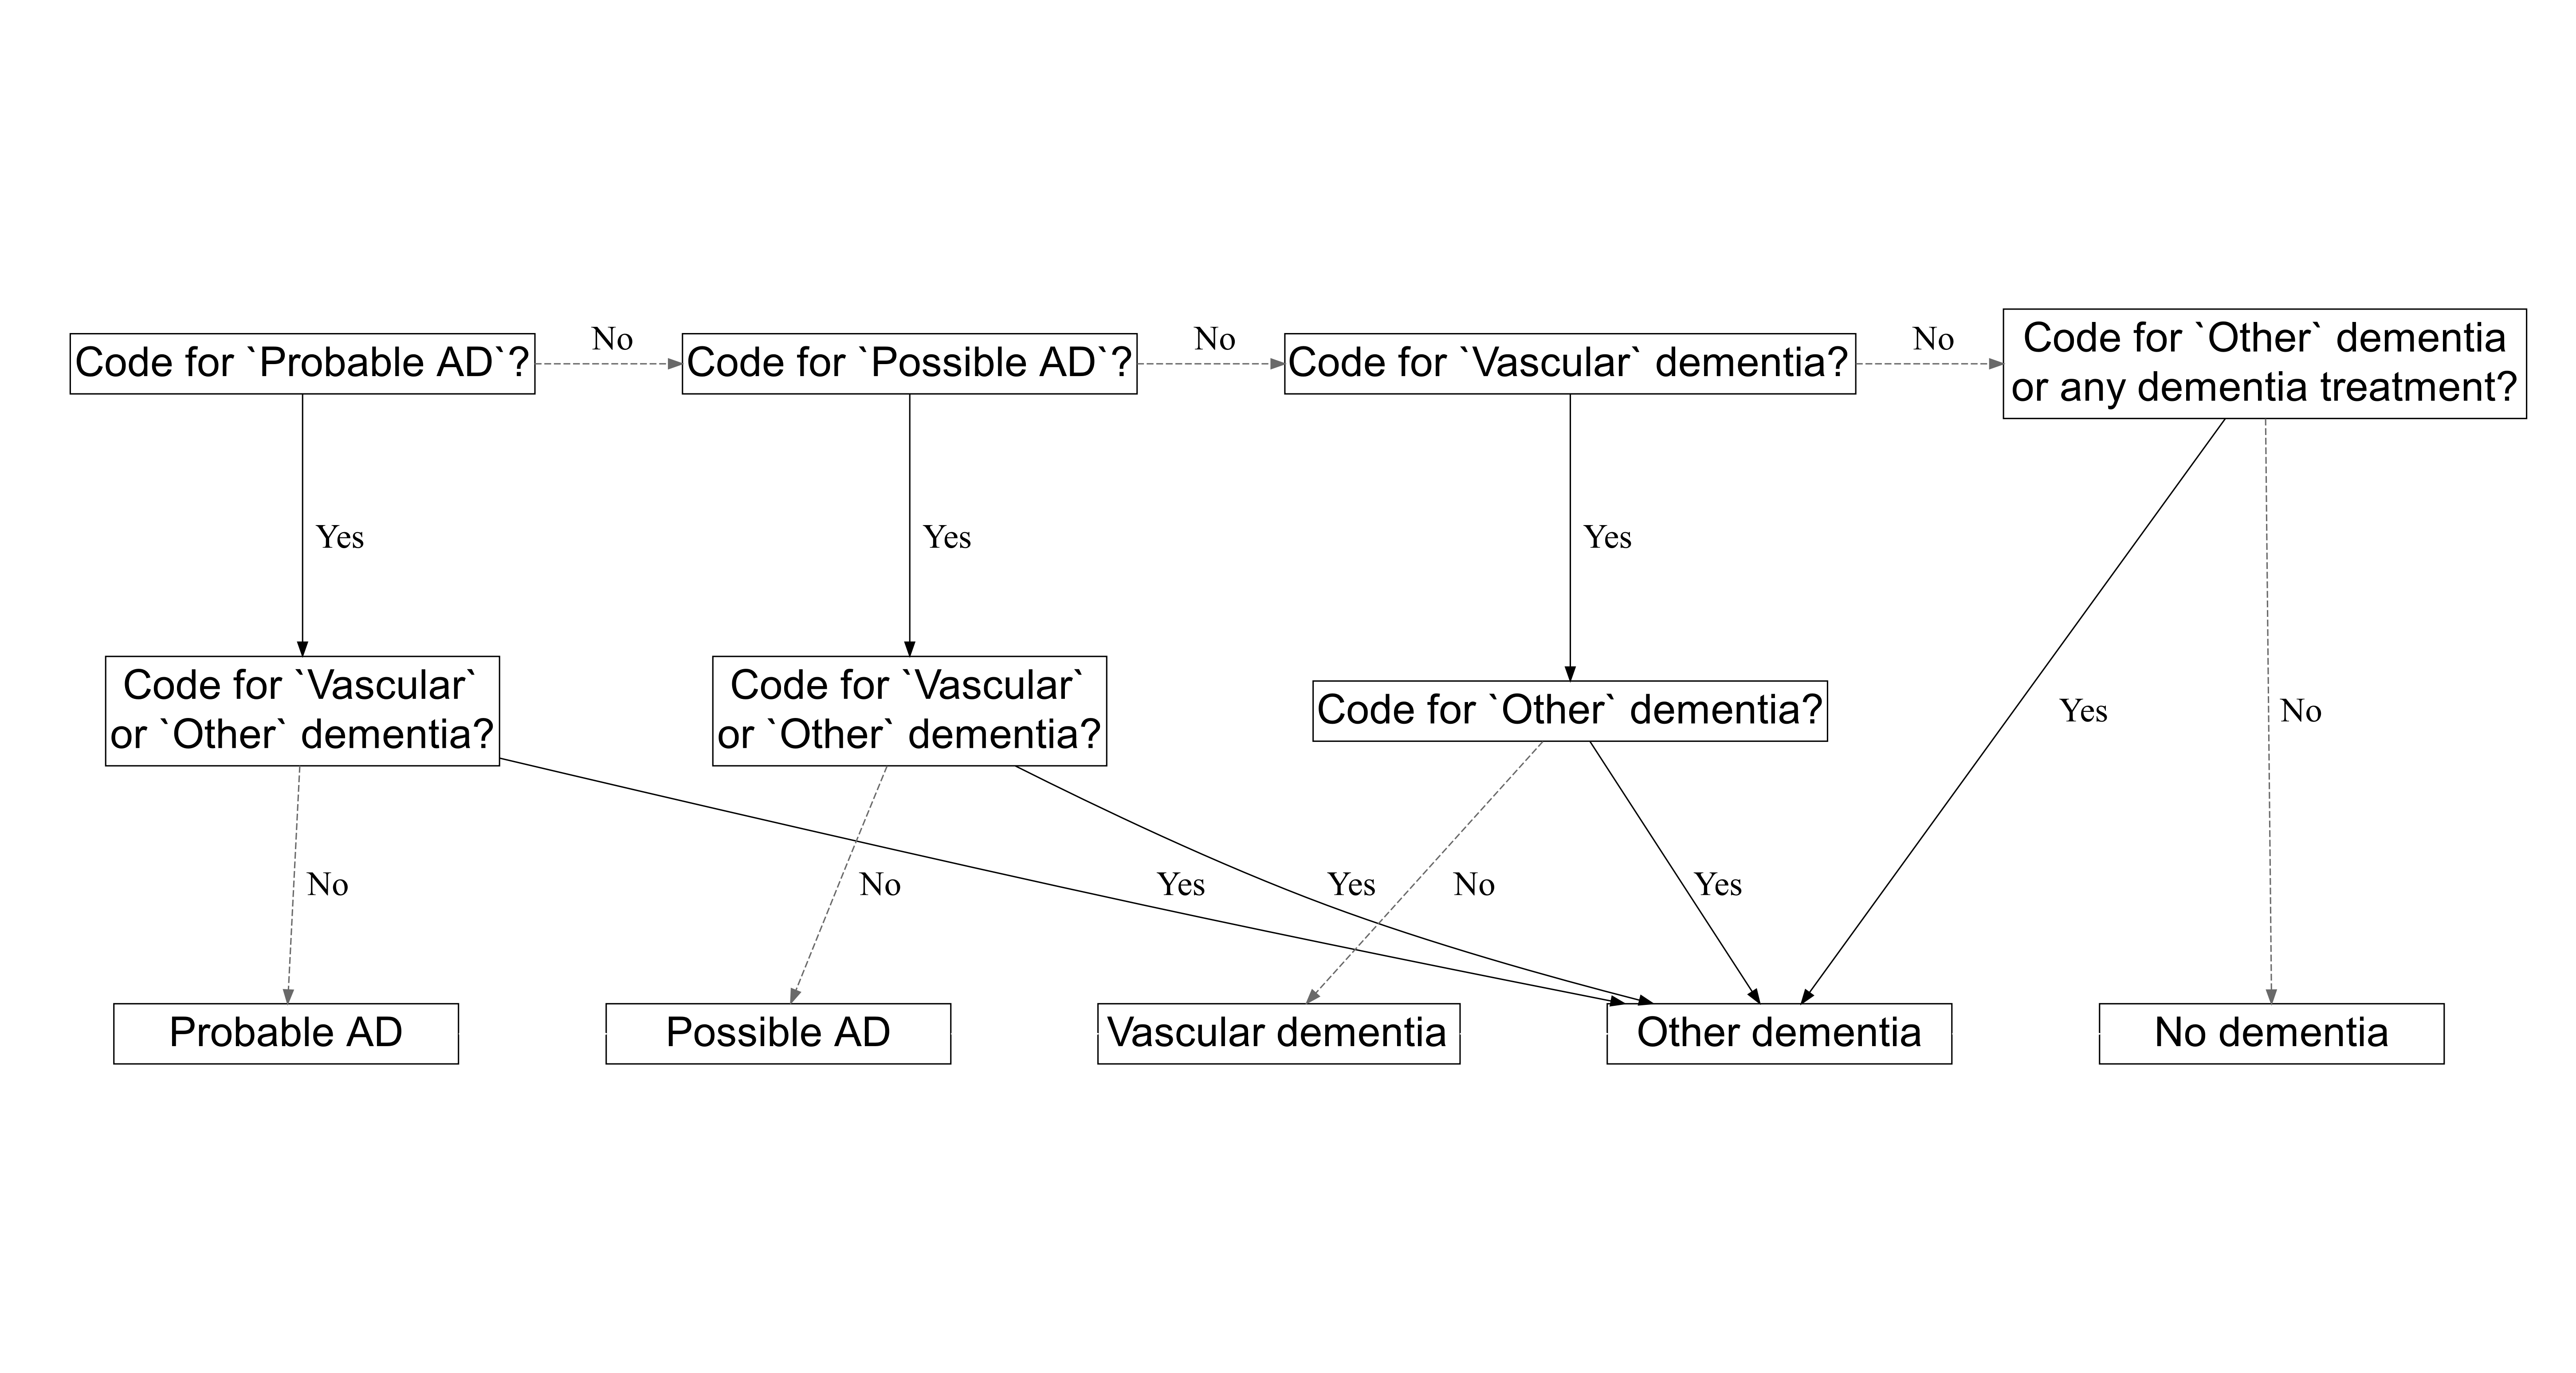
\includegraphics[width=1\linewidth]{figures/cprd-analysis/decision_tree} \caption[Decision tree for assigning dementia subtypes]{Decision tree for assigning dementia subtypes, based on the presence of Read codes in the patient's record. Note that an outcome of ``Probable'' or ``Possible'' Alzheimer's disease (AD) requires the absence of any vascular outcome codes.}\label{fig:decisionTreeFig}
\end{figure}

Participants were censored at the earliest of date of: diagnosis; death; transfer out of the study cohort; or end of follow-up (29th February 2016).

~

\hypertarget{covariates}{%
\subsection{Covariates}\label{covariates}}

A range of additional variables were included in the analysis, intended to address the different distributions of potential confounding variables between those who were prescribed an lipid-regulating agent and those who were not.

Demographic covariates adjusted for included age and gender. Age was calculated at date of entry into the cohort. Socioeconomic status was proxied using the Index of Multiple Deprivation (IMD) 2010, which draws on seven domains (income; employment; education, skills and training; health and disability; crime; barriers to housing and services; living environment) to create an overall deprivation score for each of 32844 statistical geography areas in England. To help preserve patient privacy, IMD score is only available from the CPRD in twentiles, with 1 indicating the least deprived and 20 indicating the most deprived. Smoking and alcohol use was determined at index, and participants were categorised as current, former, or never users of each.

Body mass index (a summary measure calculated as \(weight/height^2\)), baseline total cholesterol and baseline LDL cholesterol measures were obtained, using the last recorded value prior to the index date. A variable indicating grouped year of entry into the cohort (\textless2000, 2000-2004, 2005-2009, \textgreater2010) was included to allow for changes in prescribing trends across the lifetime of the cohort. To assess healthcare utilisation, I adjusted for the average annual number of consultations between the beginning of a patients data and their entry into the cohort.

Finally, presence of a range of related conditions at baseline were accounted for, including cardiovascular disease, coronary bypass surgery, coronary artery disease, peripheral arterial disease, hypertension, chronic kidney disease, and Type 1 and Type 2 diabetes. In addition to adjusting for these covariates individually, a Charlson co-morbidity index (CCI) score was calculated for each participant. The CCI is a weighted index that uses presence and severity of a number of conditions to enable adjustment for the general health of a participant in terms of their mortality risk.\textsuperscript{\protect\hyperlink{ref-charlson1987new}{184}} Inclusion of this index allowed me to attempt to adjust for the general health of patients included in the analysis.

Codelists for all covariates can be found in the archived data repository accompanying this analysis (see Section \ref{cprd-data-avail}).

~

\hypertarget{missing-data}{%
\subsection{Missing data}\label{missing-data}}

Missing data are a recognised issue in electronic health records databases,\textsuperscript{\protect\hyperlink{ref-wells2013strategies}{185}} given that they contain administrative data, collected primarily for the purposes of patient management and care rather than academic research.

In this analysis, missing data were handled using a multiple imputation approach. Variables with missing observations were identified, and 20 imputed datasets were created.\textsuperscript{\protect\hyperlink{ref-sterne2009a}{186}} Nominal variables with missing values were modelled using multinomial logistic regression, while continuous variables were modelled using linear regression. As per best practice, all variables used in the analytic model, including the outcome, were included in the imputation model.\textsuperscript{\protect\hyperlink{ref-moons2006using}{187}} Imputation was performed using the MICE (Multiple Imputation by Chained Equations) command in STATA16.

Missing data was only considered an issue for variables where a numerical test result was expected (e.g.~BMI), or where a code existed for the absence of the condition (e.g.~categorical smoking status). This approach was necessary, as absence of a code for other treatments or conditions (e.g.~statin use or dementia) was assumed to indicate absence of the treatment/condition, rather than being considered missing.\textsuperscript{\protect\hyperlink{ref-wells2013strategies}{185}}

Using multiple imputation to handle missing data is an alternative to a ``complete case'' approach,\textsuperscript{\protect\hyperlink{ref-pigott2001review}{188}} where participants missing any covariate are dropped from the dataset. As a sensitivity analysis, I preformed and compared the results of both methods,\textsuperscript{\protect\hyperlink{ref-hughes2019a}{189}} to investigate the impact of multiple imputation on the results.

~

\hypertarget{estimation-methods}{%
\subsection{Estimation methods}\label{estimation-methods}}

A Cox proportional hazards (PR) model was used to estimate the effect of statins on dementia outcomes. Cox PR models are defined, in general terms, as:

\[h(t) = h_o(t) \times exp(b_1x_1 + b_2x_2 + ... +b_px_p)\]

where:

\begin{itemize}
\tightlist
\item
  \(t\) is the survival time;
\item
  \(h(t)\) is the hazard function; and
\item
  \(x_1,x_2,...,x_p\) are the covariates which determine the hazard function, while \(b_1,b_2,...,b_p\) are the coefficients for each covariate.
\item
  \(h_o(t)\) is the baseline hazard - when all \(x_i\) are zero, the \(exp()\) function resolves to 1.
\end{itemize}

As the values of \(b_i\) increases, value of \(exp(b_i)\) (i.e.~the hazard ratio) increases in tandem, thus reducing the survival time, \(t\).

A Cox PR model was chosen for this analysis as it inherently accounts for the length of time participants spend in each exposure group. Using this approach, time-at-risk can be properly attributed, thus mitigating the impact of immortal time bias. This is discussed in detail in the following section.

~

\hypertarget{cprd-immortal-time-bias}{%
\subsection{Immortal time bias and time-varying treatment indicators}\label{cprd-immortal-time-bias}}

Immortal time bias covers two distinct but related types of bias. The first presentation, the selection bias aspect (Panel A, Figure \ref{fig:immortalTimeBias}), occurs when time prior to the exposure is excluded leading to the exposed and control groups being followed up from different time points.\textsuperscript{\protect\hyperlink{ref-levesque2010a}{190}} For example, if the unexposed group are followed from a cholesterol test result, while the exposed group is followed from date of LRA prescription, any events that occur in the exposed group prior to the exposure event will be inappropriately excluded from the analysis.

The second presentation of immortal time bias is as a type of misclassification bias (Panel B, Figure \ref{fig:immortalTimeBias}). It occurs when the exposure time prior to the exposure date, and any events occurring within it, is inappropriately assigned to the exposed group. This second presentation appears to be common in the existing literature, as several of the studies included in the systematic review presented in Chapter \ref{sys-rev-heading} were identified as being at risk of immortal time bias following formal risk of bias assessment using the ROBINS-I tool (see Section \ref{risk-of-bias-subheading}).

This analysis is primarily concerned with the second presentation of immortal time bias, as all participants were followed from a common index date (earliest of: date of raised cholesterol test results; hypercholesterolemeia diagnosis; or LRA prescription). To address the potential for this second form of immortal time bias in the analysis, I employed a time-varying indicator of treatment status to correctly allocate time-at-risk to the exposed and unexposed groups.\textsuperscript{\protect\hyperlink{ref-levesque2010}{191}}

Under this approach, all patients start in the unexposed group, \& contribute time-at-risk until they are prescribed a lipid regulating agent and move into the exposed group. Note, patients for whom prescription of a lipid regulating agent was the index event only contribute time to the exposed group (i.e.~they enter the cohort and move into the exposed group on the same day).





\begin{figure}[H]
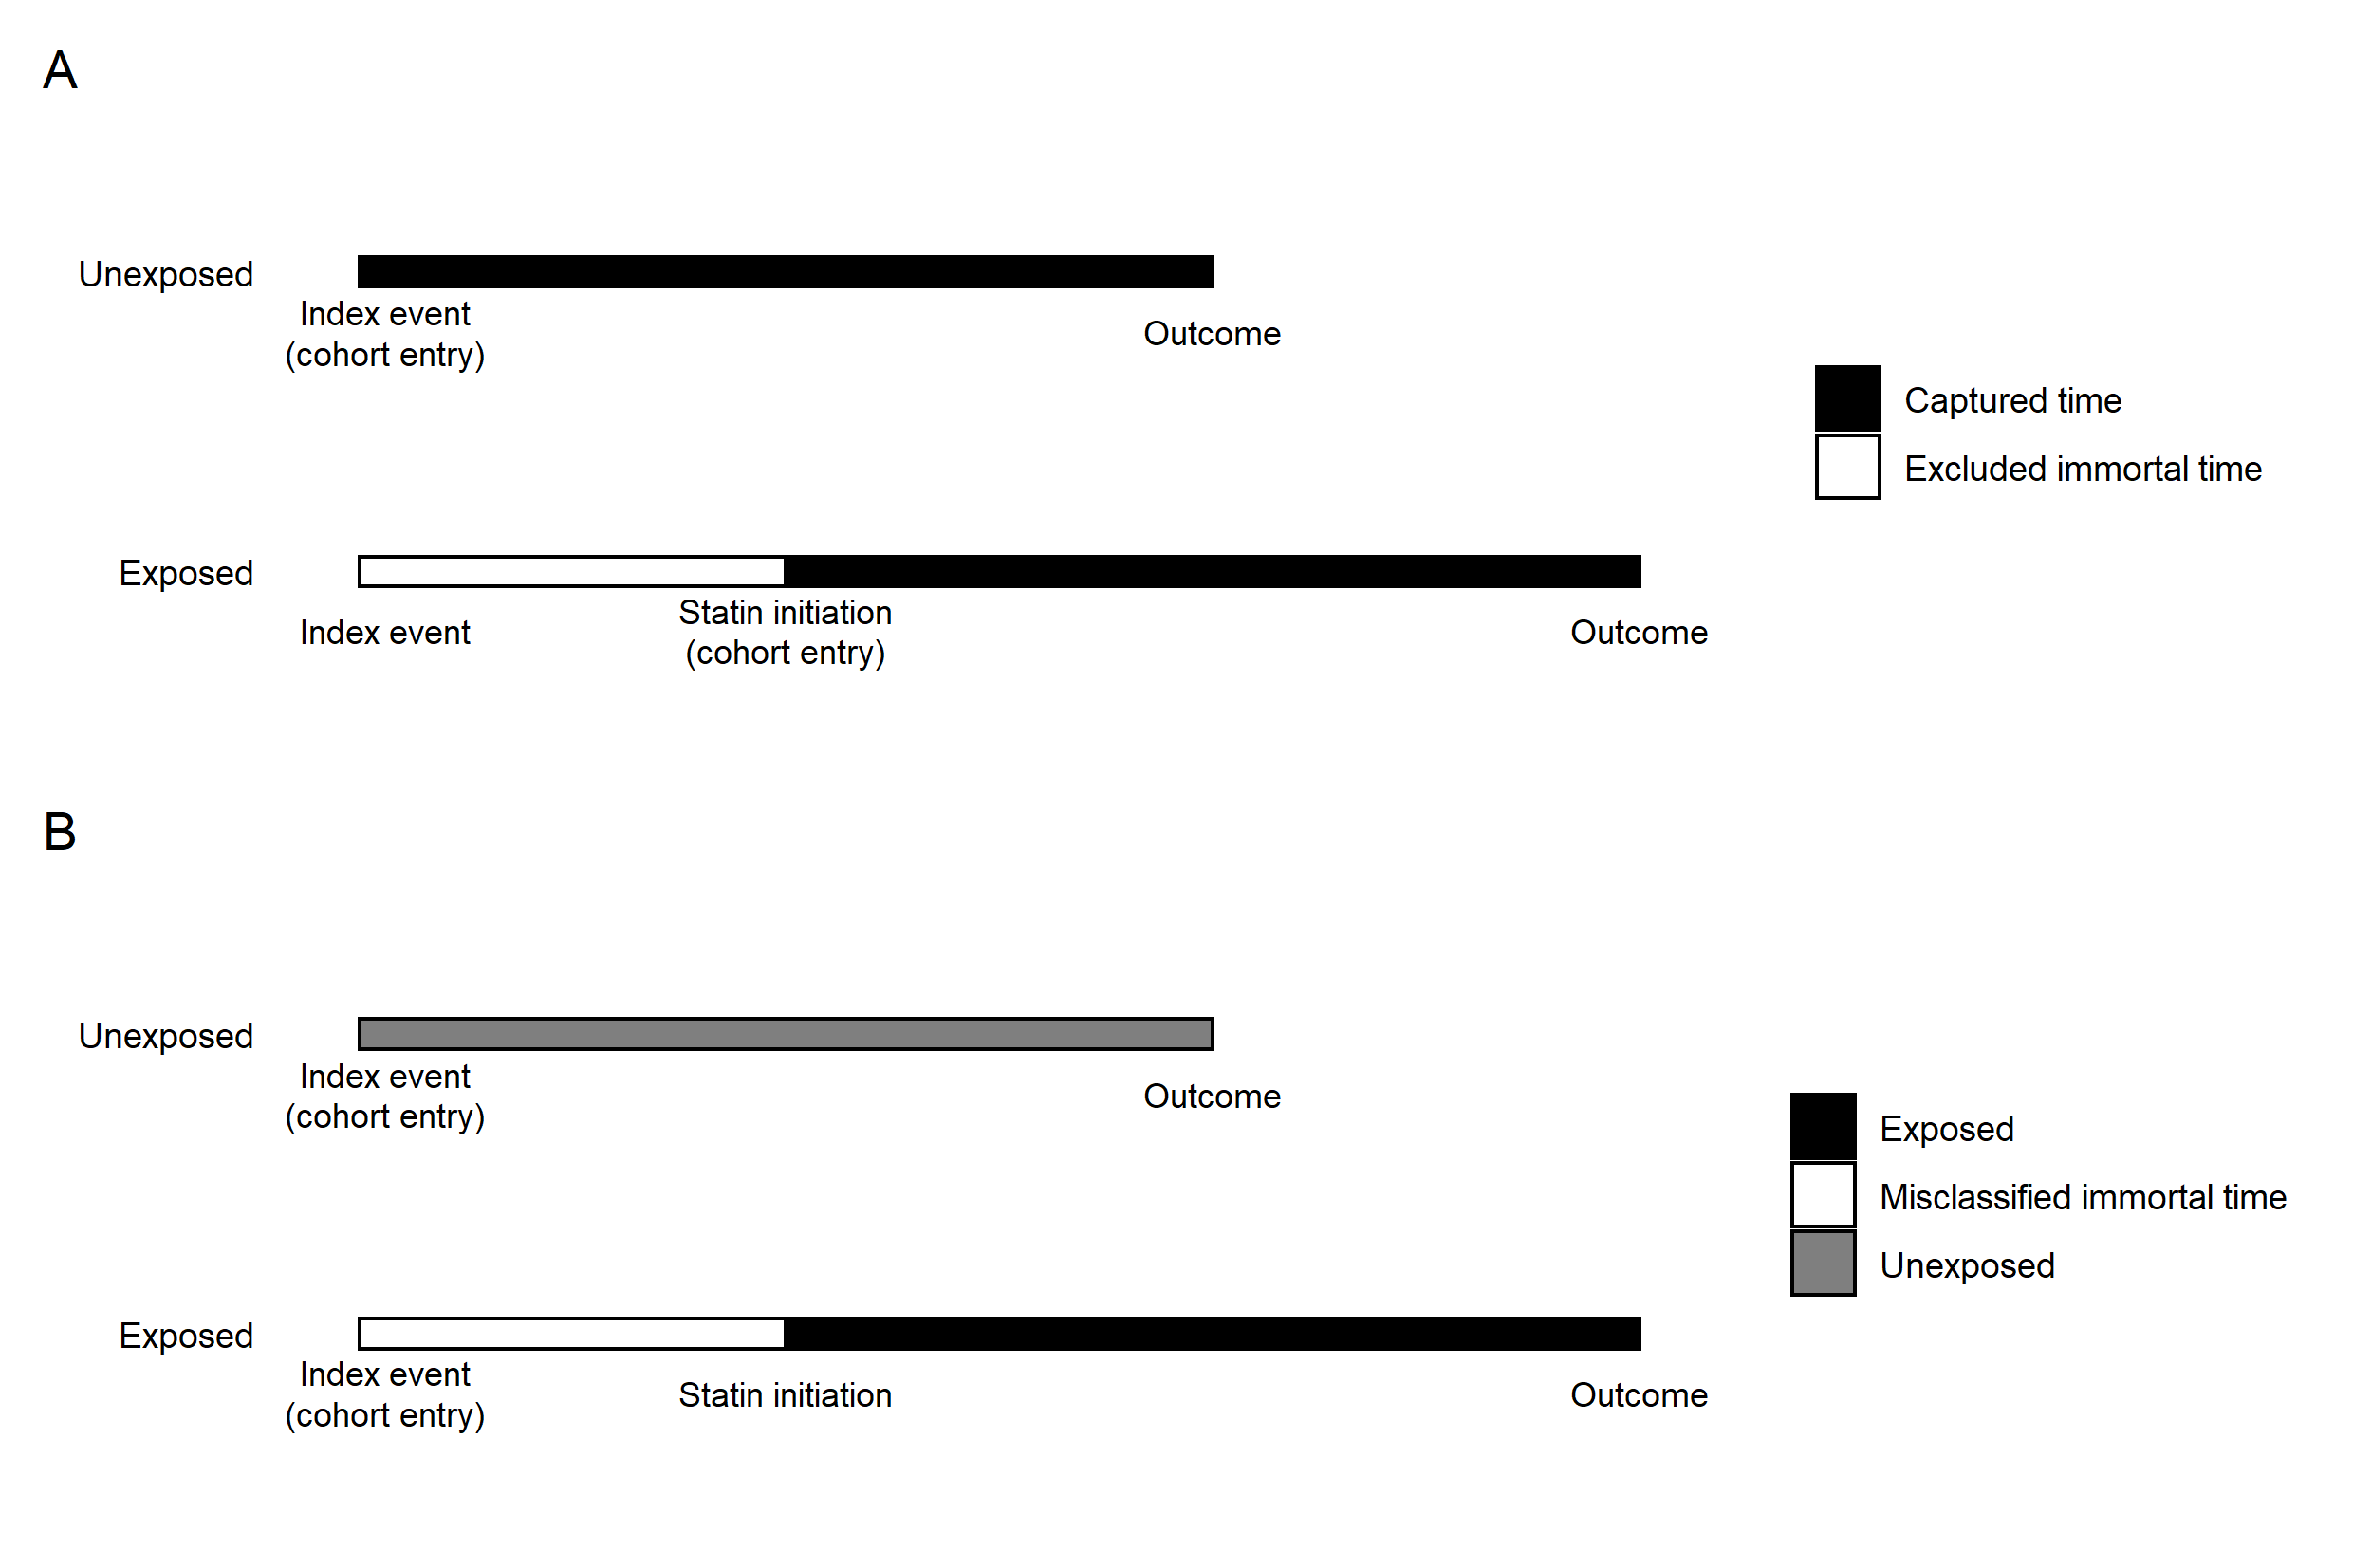
\includegraphics[width=1\linewidth]{figures/cprd-analysis/immortal_time} \caption[shortcap]{Diagram illustrating the two presentations of immortal time bias, as a selection bias (Panel A) and a misclassification bias (Panal B).}\label{fig:immortalTimeBias}
\end{figure}

\hypertarget{time-axis}{%
\subsection{Time axis}\label{time-axis}}

As part of a Cox proportional hazard model, there is the option to use either absolute time in cohort or participants age as the time scale of interest.\textsuperscript{\protect\hyperlink{ref-lamarca1998}{192}--\protect\hyperlink{ref-pencina2007}{194}} A model using age as the time axis inherently accounts, or adjusts, for participants age as a potential confounded of the exposure-outcome relationship. The main analyses presented all used age as the time axis.

~

\hypertarget{sensitivity-analyses-1}{%
\subsection{Sensitivity analyses}\label{sensitivity-analyses-1}}

The primary analysis examined the effect of a lipid regulating agent on dementia risk, stratified by outcome and drug class. To assess the robustness of the results, a number of sensitivity analyses were performed. These are described in the following sections.

\hypertarget{control-outcomes}{%
\subsubsection{Control outcomes}\label{control-outcomes}}

In addition to the primary outcomes of interest (described in Section \ref{cprd-outcomes}), I extracted data on two additional control outcomes. The inclusion of control outcomes in observational analyses are a useful technique to assess the strength of uncontrolled confounding,\textsuperscript{\protect\hyperlink{ref-lipsitch2010}{195}} and these outcomes are usually class as either ``negative'' or ``positive'' outcomes. Negative outcomes are those without a likely causal path between the exposure and outcome (see Figure \ref{fig:negativeOutcome} for a directed acyclic graph describing an ideal negative outcome).

Conversely, positive control outcomes are those with a known causal association with the exposure of interest, ideally sourced from large well conducted randomised controlled trials. Positive control outcomes are useful in observational epidemiology, as if the analysis can reproduce a known result for the control outcome, confidence in the result for the outcome of interest is increased.

Due to the wealth of data available on statins as a lipid regulating agent, control outcomes were chosen in reference to this drug class. Muscular backpain was chosen as a negative control outcome in this analysis. Despite observational analyses suggesting a link between statins and muscle pain (as opposed to more serious complications such as myopathy),\textsuperscript{\protect\hyperlink{ref-selva-ocallaghan2018}{196}} systematic reviews of the adverse events of statin use\textsuperscript{\protect\hyperlink{ref-collins2016a}{36}} and N-of-1 trials explicitly exploring the effect of statin use on muscle pain\textsuperscript{\protect\hyperlink{ref-herrett2021}{197}} have found no evidence of an effect. As such, if no evidence of an effect of statins on backpain is found in the analysis, then confidence in the results for the dementia outcomes is increased.

Additionally, incident ischemic heart disease was included as a positive control outcome, given the well-established protective effect of lipid-lowering treatment, via statins, on the risk of this condition.\textsuperscript{\protect\hyperlink{ref-collins2016a}{36}} Similar to the backpain outcome, if the analysis strategy can reproduce this known protective association, this will provide evidence that potential confounders have been sufficiently adjusted for.





\begin{figure}[H]
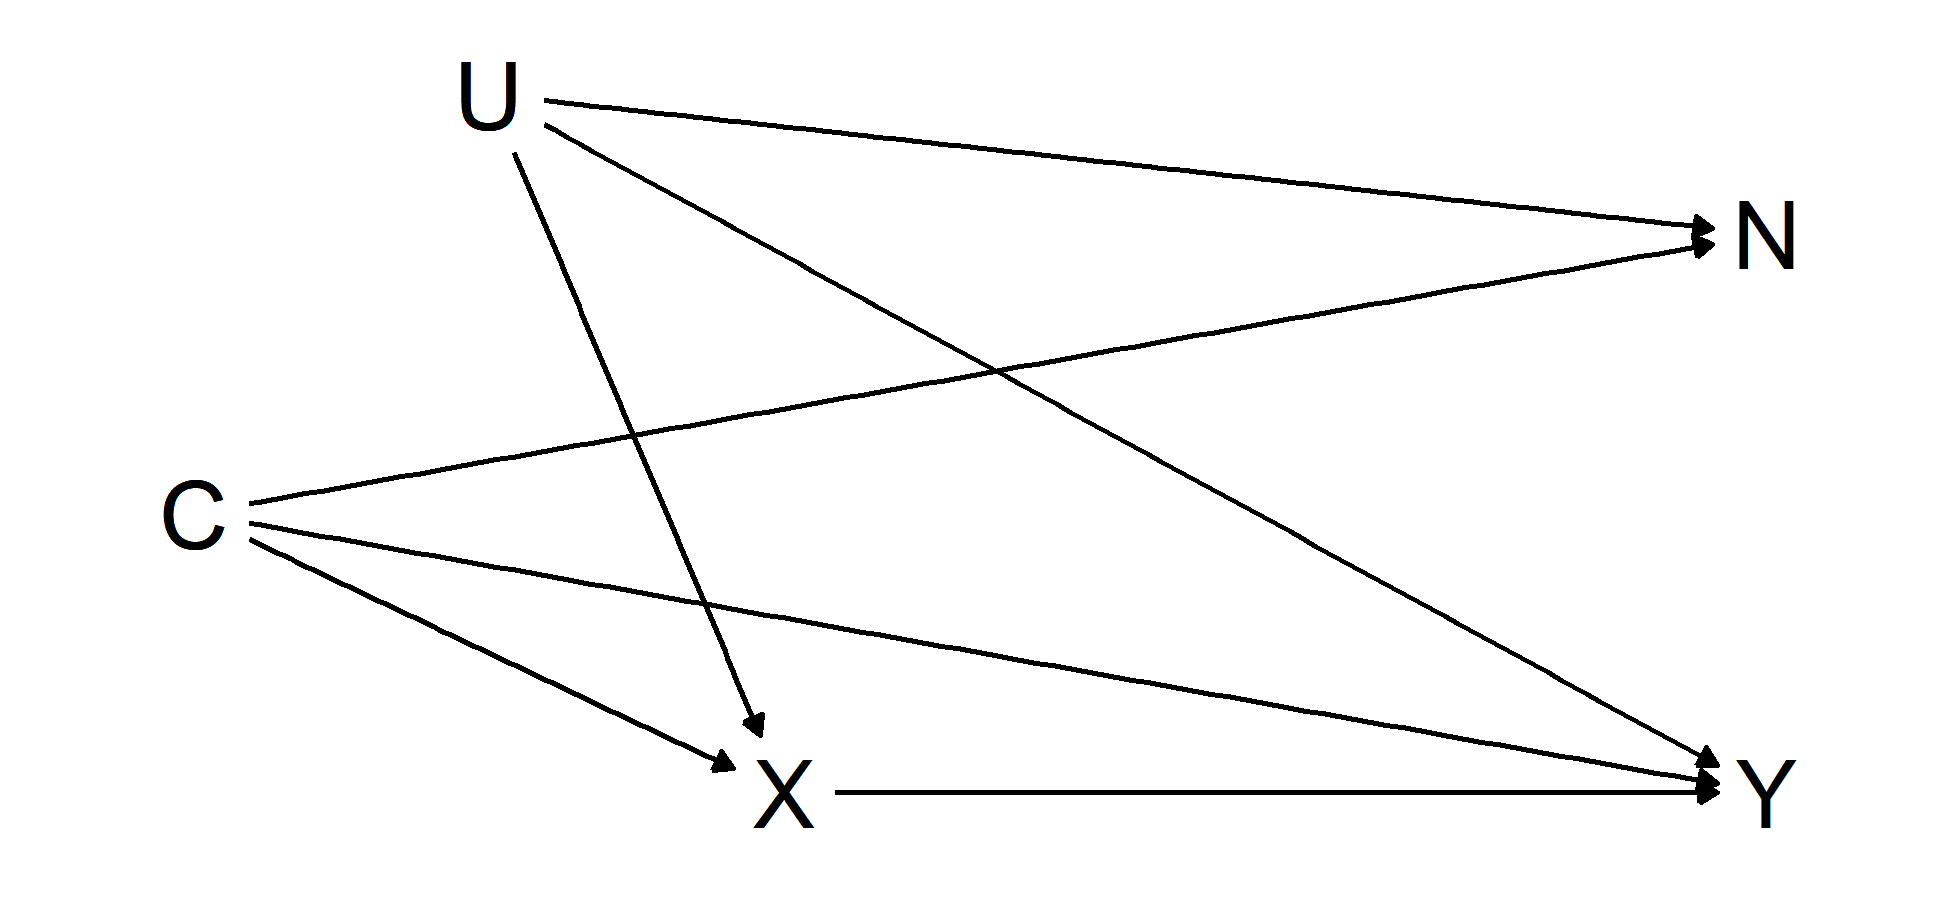
\includegraphics[width=1\linewidth]{figures/cprd-analysis/negativeOutcome} \caption[DAG of ideal negative outcome]{Causal diagram showing relationship between exposure \(X\), outcome \(Y\), confounders (measured \(C\) and unmeasured \(U\)) and an ideal negative outcome \(N\). Note the absence of any arrow between \(X\) and \(N\). In this scenario, any association observed between \(X\) and \(N\) is due to the presence of uncontrolled confounders \(U\) (assuming \(C\) has been adjusted for).}\label{fig:negativeOutcome}
\end{figure}

\hypertarget{impact-of-additional-covariates}{%
\subsubsection{Impact of additional covariates}\label{impact-of-additional-covariates}}

To observe the effect of adjusting for additional covariates, I ran a model unadjusted except for age (captured via the time axis in the Cox model) and gender, and compared the results with the full adjusted model.

~

\hypertarget{sensitivity-cohorts}{%
\subsubsection{Sensitivity cohorts}\label{sensitivity-cohorts}}

Two sensitivity cohorts were also created. The first stratified by year of entry into the cohort in an attempt to assess for time period effects. The second removed participants who may have been pregnant (coded as under 55 and female) to assess the robustness of the estimates, as statins are contraindicated in pregnancy, .\textsuperscript{\protect\hyperlink{ref-karalis2016}{198}}

~

\hypertarget{statin-properties}{%
\subsubsection{Statin properties}\label{statin-properties}}

As detailed in the introduction, the properties of statins may be important in their effect, based on the ability of lipophilic statins to cross the blood brain barrier (see Section \ref{intro-statins} in the Introductory Chapter).

To explore whether any observed effect for the statin analysis varied by statin property, a sensitivity analysis was performed, stratifying by statin lipophilicity.

~

\hypertarget{impact-of-dementia-code-lists}{%
\subsubsection{Impact of dementia code lists}\label{impact-of-dementia-code-lists}}

As part of an exploratory analysis of the effect of the choice of code lists on the analysis, I created an alternative Alzheimer's disease and non-Alzheimer's dementia outcome using code lists from a previous study published in 2009 by Smeeth \emph{et al}.\textsuperscript{\protect\hyperlink{ref-smeeth2009}{199}}

This previous study used a propensity matching approach to estimate the effect of statins on a range of outcomes, and a protective effect of statin use on all-cause dementia (HR: 0.81, 95\% CI: 0.69-0.96) and non-AD dementia (HR: 0.82, 95\% CI: 0.69-0.97), but no evidence of an effect on AD (HR: 0.81, 95\% CI: 0.49-1.35).

The code lists used were obtained through correspondence with the authors of that study, and are available for inspection (see Section \ref{cprd-data-avail}).

~

\hypertarget{results-1}{%
\section{Results}\label{results-1}}

\hypertarget{patient-characteristics}{%
\subsection{Patient characteristics}\label{patient-characteristics}}

Of the 3,179,733 participants included in the extract, 1,684,564 met the inclusion criteria (Figure \ref{fig:cprdFlowchart}), with a total follow-up of 10,800,903 patient years at risk.

~





\begin{figure}[H]
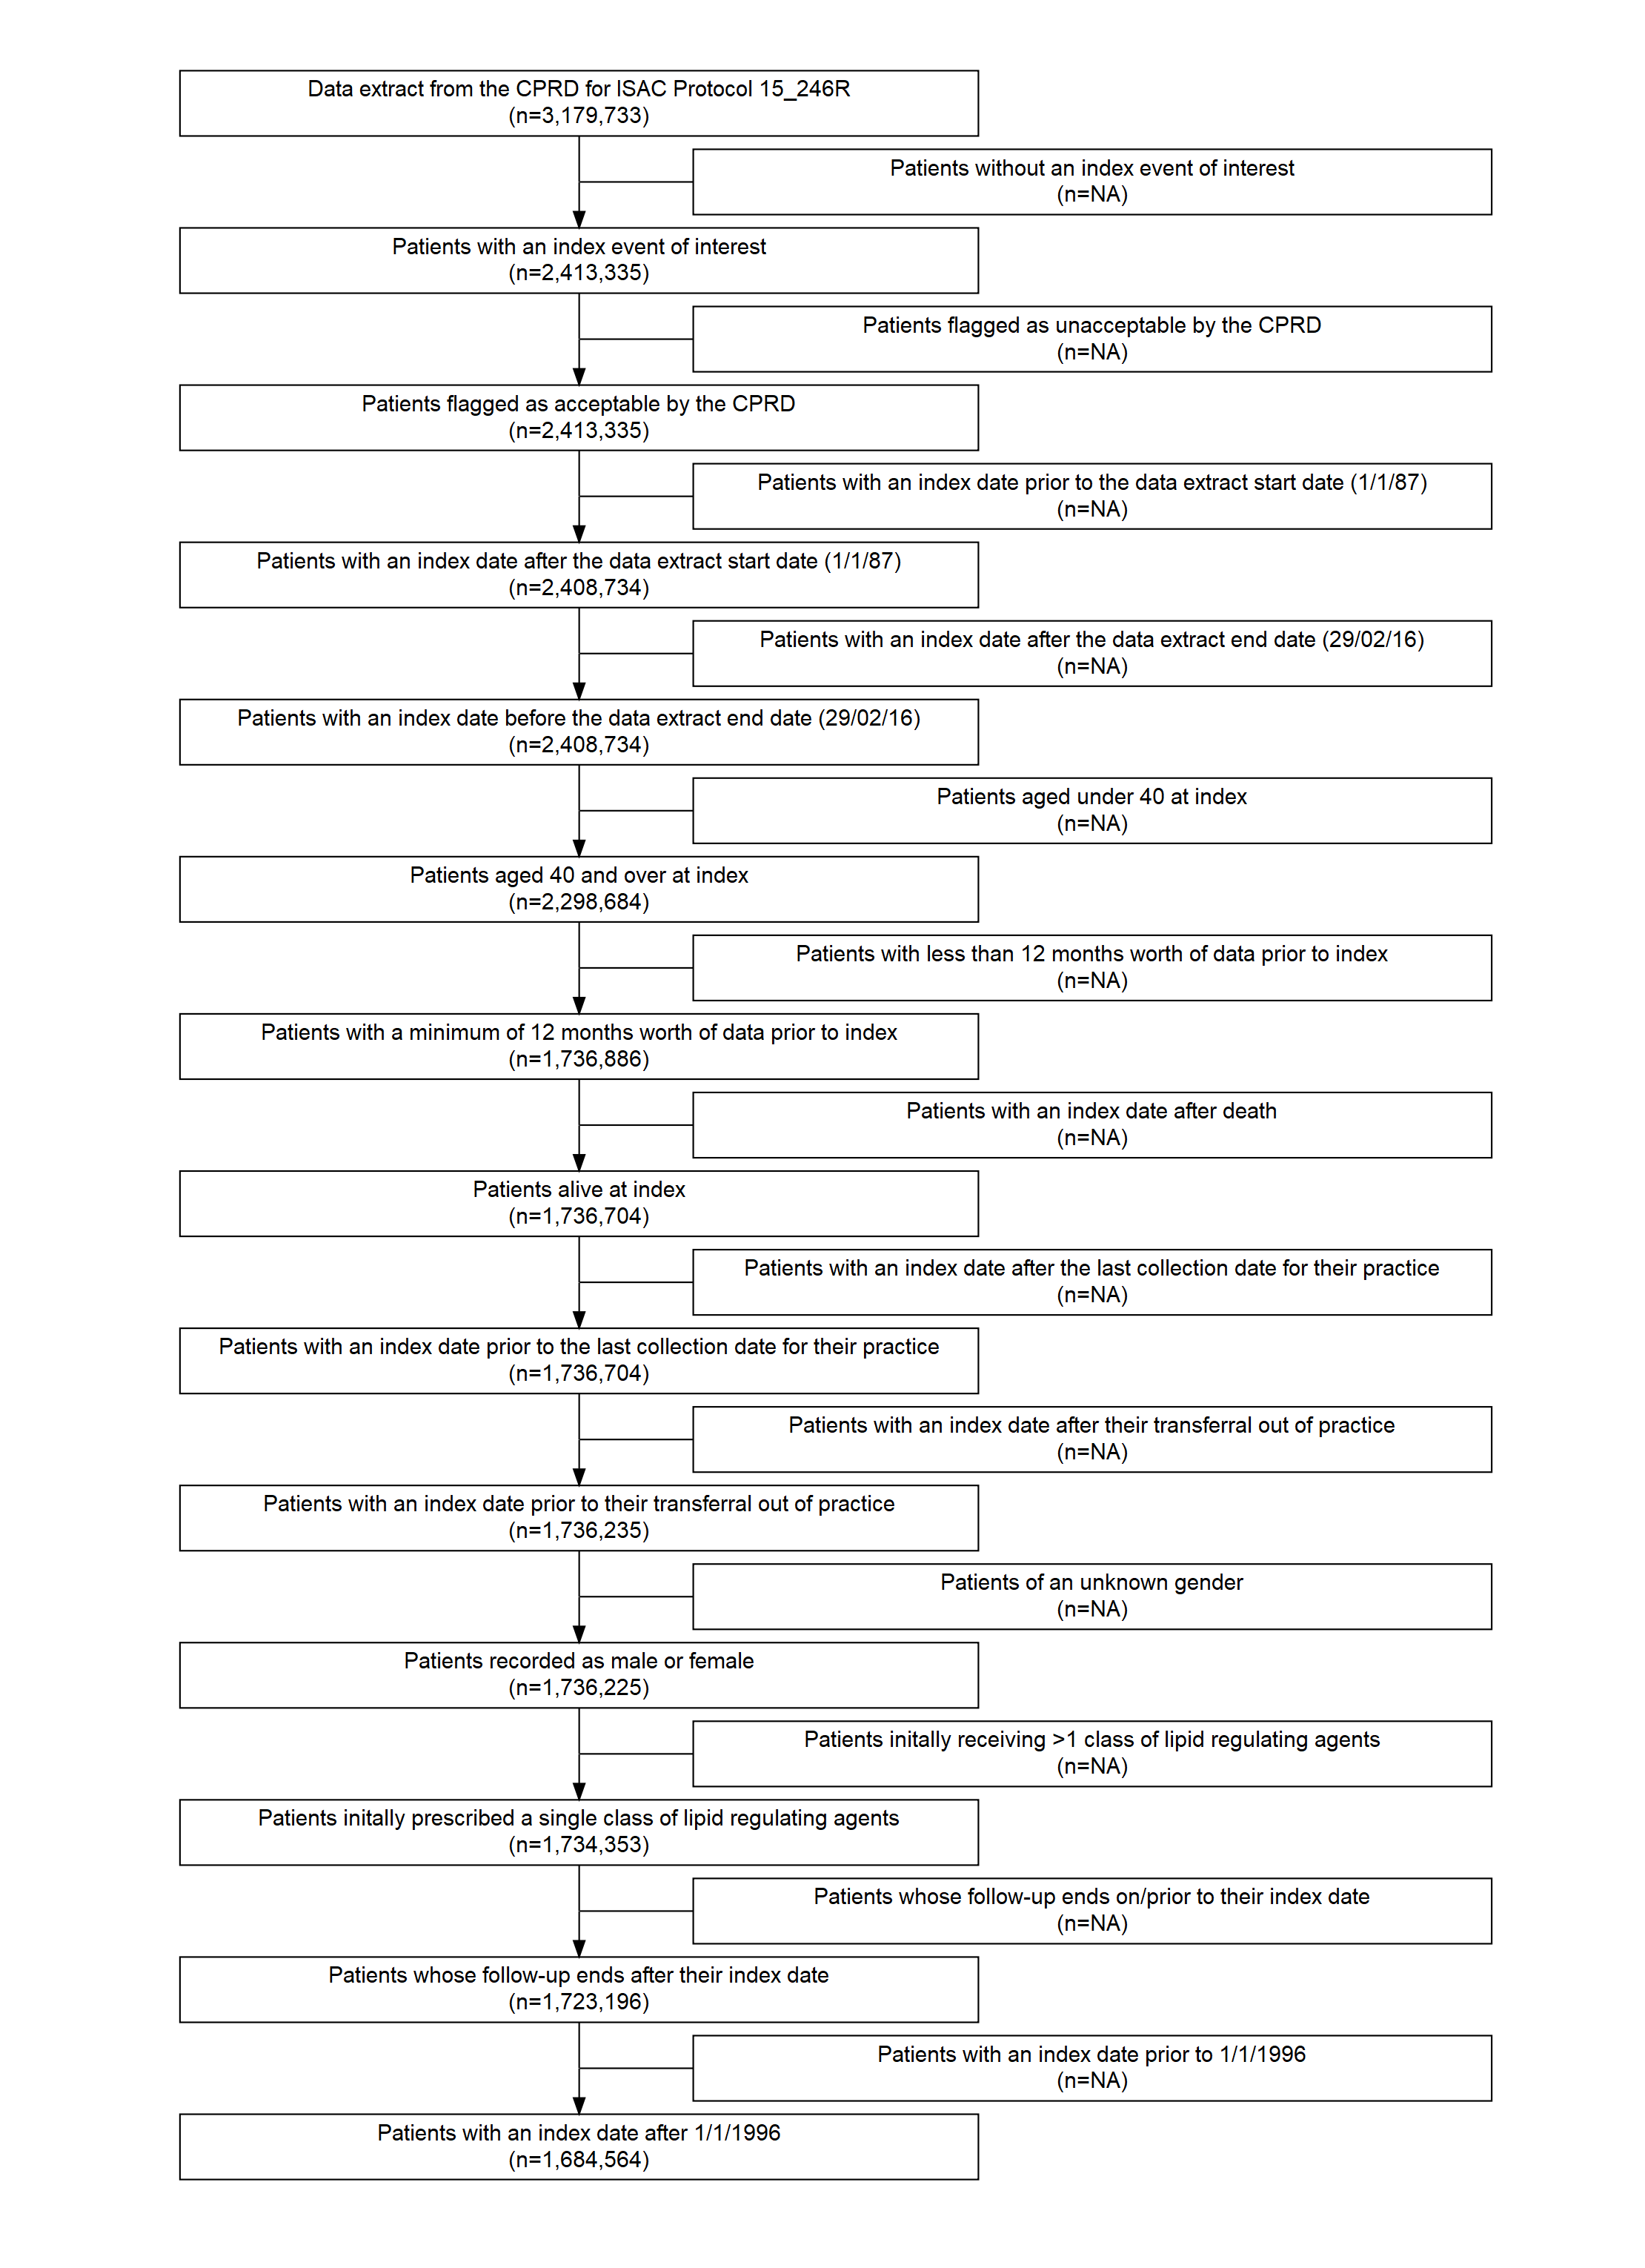
\includegraphics[width=1\linewidth]{figures/cprd-analysis/cohort_attrition} \caption[Attrition of CPRD participants]{Attrition of CPRD participants as the eligibility criteria were applied. Most attrition was due to the absence of an index event of interest.}\label{fig:cprdFlowchart}
\end{figure}

~

The median participant age at index was 57 years (Inter quartile range (IQR):48-68) and participants were followed up for a median of 5.8 years (IQR:2.7-9.7). During follow-up, an all-cause dementia diagnosis was recorded for 41,830 patients (12,647 probable AD, 9,954 possible AD, 8,466 vascular dementia, 10,763 other dementia). The distribution of baseline characteristics across the seven drug classes can be seen in Table \ref{tab:cprdCharacteristics-table}.

\blandscape





\begin{table}[H]

\caption[Patient characteristics by drug class]{\label{tab:cprdCharacteristics-table}Patient characteristics by drug class. Summary statistics are presented as ``\% (N)'' unless otherwise specified in the variable name.}
\centering
\fontsize{5}{7}\selectfont
\begin{threeparttable}
\begin{tabular}[t]{>{\raggedright\arraybackslash}p{10em}>{\centering\arraybackslash}p{6em}>{\centering\arraybackslash}p{6em}>{\centering\arraybackslash}p{6em}>{\centering\arraybackslash}p{6em}>{\centering\arraybackslash}p{6em}>{\centering\arraybackslash}p{6em}>{\centering\arraybackslash}p{6em}>{\centering\arraybackslash}p{6em}>{\centering\arraybackslash}p{6em}}
\toprule
\textbf{ } & \textbf{Whole Sample} & \textbf{None} & \textbf{Statins} & \textbf{Bile acid sequestrants} & \textbf{Ezetimibe} & \textbf{Ezetimibe \& Statins} & \textbf{Fibrates} & \textbf{Nicotinic acid groups} & \textbf{Omega-3 Fatty Acid Groups}\\
\midrule
\textbf{Sample size (N)} & 1695683 & 1095857 & 588455 & 5417 & 766 & 127 & 3896 & 168 & 997\\
\midrule
\textbf{Index year \newline(median)} & 2006 & 2007 & 2004 & 2005 & 2004 & 2005 & 2001 & 2001 & 2005\\
\midrule
\textbf{Female} & 53.1\% (900847) & 56.3\% (616801) & 47.2\% (277841) & 66.4\% (3598) & 54.6\% (418) & 52.8\% (67) & 38.6\% (1505) & 54.8\% (92) & 52.7\% (525)\\
\midrule
\textbf{Age} & 57 & 54 & 62 & 57 & 60 & 57 & 58 & 62 & 56\\
\midrule
\textbf{CAD} & 0.4\% (7180) & 0.1\% (614) & 1.1\% (6487) & 0.1\% (6) & 0.9\% (7) & 0.0\% (0) & 1.4\% (53) & 0.0\% (0) & 1.3\% (13)\\
\midrule
\addlinespace
\textbf{CBS} & 0.3\% (5739) & 0.1\% (701) & 0.8\% (4947) & 0.1\% (4) & 0.4\% (3) & 0.0\% (0) & 2.0\% (78) & 0.0\% (0) & 0.6\% (6)\\
\midrule
\textbf{CVD} & 2.2\% (36680) & 1.2\% (12803) & 4.0\% (23567) & 1.7\% (90) & 2.6\% (20) & 2.4\% (3) & 4.4\% (171) & 4.8\% (8) & 1.8\% (18)\\
\midrule
\textbf{Charlson (ever > 0)} & 31.0\% (525566) & 25.5\% (279520) & 40.9\% (240925) & 42.6\% (2308) & 41.8\% (320) & 24.4\% (31) & 50.9\% (1983) & 44.6\% (75) & 40.5\% (404)\\
\midrule
\textbf{IMD-2010 (median)} & 9 & 8 & 9 & 8 & 9 & 13 & 10 & 11 & 10\\
\midrule
\textbf{Consulation rate (mean/SD)} & 5.4 (5.5) & 5.0 (5.0) & 6.3 (6.1) & 8.6 (7.4) & 7.4 (6.6) & 4.8 (4.3) & 7.1 (6.2) & 9.3 (7.7) & 8.0 (8.0)\\
\midrule
\addlinespace
\textbf{Alcohol (ever)} & 85.8\% (1455443) & 86.5\% (947716) & 84.7\% (498304) & 82.8\% (4487) & 83.9\% (643) & 87.4\% (111) & 82.8\% (3226) & 82.7\% (139) & 81.9\% (817)\\
\midrule
\textbf{Smoking (ever)} & 51.1\% (866207) & 47.0\% (515192) & 58.5\% (344540) & 55.2\% (2990) & 57.4\% (440) & 60.6\% (77) & 60.1\% (2342) & 53.6\% (90) & 53.8\% (536)\\
\midrule
\textbf{BMI (mean/SD)} & 27.0 (5.3) & 26.7 (5.2) & 27.7 (5.3) & 26.8 (5.8) & 28.1 (5.7) & 28.1 (4.9) & 29.0 (5.2) & 26.4 (5.0) & 26.8 (5.5)\\
\midrule
\textbf{PAD} & 0.8\% (12879) & 0.4\% (4204) & 1.4\% (8524) & 0.9\% (47) & 0.9\% (7) & 0.8\% (1) & 1.9\% (75) & 6.5\% (11) & 1.0\% (10)\\
\midrule
\textbf{Hypertension} & 16.1\% (273011) & 11.6\% (126891) & 24.5\% (144010) & 12.9\% (697) & 23.9\% (183) & 25.2\% (32) & 25.8\% (1006) & 21.4\% (36) & 15.6\% (156)\\
\midrule
\addlinespace
\textbf{Total cholesterol (mean/SD)} & 5.7 (12.4) & 5.5 (10.8) & 6.2 (15.3) & 5.3 (1.3) & 7.1 (26.5) & 6.7 (1.5) & 6.4 (5.6) & 5.4 (1.5) & 5.6 (1.7)\\
\midrule
\textbf{LDL cholesterol (mean/SD)} & 3.6 (4.8) & 3.4 (5.2) & 4.0 (3.6) & 3.1 (1.0) & 3.9 (1.1) & 4.2 (1.0) & 3.3 (1.8) & 3.4 (0.9) & 3.2 (1.0)\\
\midrule
\textbf{CKD} & 0.1\% (1391) & 0.1\% (814) & 0.1\% (566) & 0.1\% (7) & 0.1\% (1) & 0.0\% (0) & 0.0\% (0) & 0.0\% (0) & 0.3\% (3)\\
\midrule
\textbf{Type 1 Diabetes} & 0.2\% (4057) & 0.1\% (795) & 0.5\% (3206) & 0.3\% (14) & 1.0\% (8) & 0.8\% (1) & 0.8\% (31) & 0.6\% (1) & 0.1\% (1)\\
\midrule
\textbf{Type 2 Diabetes} & 2.9\% (49381) & 1.1\% (12376) & 6.1\% (36182) & 2.3\% (124) & 5.4\% (41) & 4.7\% (6) & 15.8\% (617) & 4.2\% (7) & 2.8\% (28)\\
\bottomrule
\end{tabular}
\begin{tablenotes}
\item \textit{Abbreviations:} 
\item LRA - Lipid regulating agent; IMD - Index of Multiple Deprivation; BMI - Body Mass Index; CAD - Coronary Arterial Disease; CBS - Coronary Bypass Surgery; CVD - Cardiovascular disease; PAD - Peripheral arterial disease; CKD - Chronic Kidney Disease; SD - Standard deviation.
\end{tablenotes}
\end{threeparttable}
\end{table}

\elandscape

A substantial majority (98.1\%) of participants prescribed a lipid-regulating agent were prescribed a statin. I excluded the ``Ezetimibe and statins'' and ``Nicotinic acid groups'' classes from subsequent analysis based on the extremely small number of participants in these groups (N=127 \& N=168 respectively; see Table \ref{tab:cprdCharacteristics-table}). Note that the ``Ezetimibe and statins'' treatment group represent those prescribed a single treatment containing both ezetimibe and statins, rather than those where the two treatments were prescribed concurrently.

~





\begin{table}[H]

\caption[Participants who stopped, switched or added treatements by initial treatment type]{\label{tab:cprdSSA-table}Participants who stopped, switched or added treatments by initial treatment type.}
\centering
\fontsize{7}{9}\selectfont
\begin{threeparttable}
\begin{tabular}[t]{>{\raggedright\arraybackslash}p{5em}>{\centering\arraybackslash}p{4.225em}>{\centering\arraybackslash}p{4.225em}>{\centering\arraybackslash}p{4.225em}>{\centering\arraybackslash}p{4.225em}>{\centering\arraybackslash}p{4.225em}>{\centering\arraybackslash}p{4.225em}>{\centering\arraybackslash}p{4.225em}>{\centering\arraybackslash}p{4.225em}}
\toprule
\textbf{ } & \textbf{Whole Sample} & \textbf{Statins} & \textbf{Bile acid sequestrants} & \textbf{Ezetimibe} & \textbf{Ezetimibe \& Statins} & \textbf{Fibrates} & \textbf{Nicotinic acid groups} & \textbf{Omega-3 Fatty Acid Groups}\\
\midrule
\textbf{Stopped} & 6.8\% (115899) & 19.0\% (111798) & 55.9\% (3028) & 19.6\% (150) & 12.6\% (16) & 12.3\% (478) & 44.0\% (74) & 35.6\% (355)\\
\midrule
\textbf{Added} & 1.6\% (27470) & 4.4\% (26018) & 3.5\% (192) & 18.9\% (145) & 3.9\% (5) & 21.6\% (841) & 4.2\% (7) & 26.3\% (262)\\
\midrule
\textbf{Switched} & 0.9\% (14956) & 2.0\% (12014) & 11.3\% (614) & 34.5\% (264) & 64.6\% (82) & 44.0\% (1714) & 44.6\% (75) & 19.4\% (193)\\
\bottomrule
\end{tabular}
\begin{tablenotes}
\item \textit{Definitions:} 
\item Stopped - last prescription of the primary drug class followed by at least six months of observation with no further prescriptions; Added - second drug class prescribed before the last prescription of the initial class; Switched - second drug class being prescribed after the last prescription of the initial class.
\end{tablenotes}
\end{threeparttable}
\end{table}

~

The stopping, addition and switching of drug classes was common across all drug classes (Table \ref{tab:cprdSSA-table}).

~

\hypertarget{missing-data-1}{%
\subsection{Missing data}\label{missing-data-1}}

Full covariate information was available for 451,897 participants (26.6\%). Six key variables had some missing data: IMD 2010 score was missing for 630,439 participants (37.2\%), because it is only recorded for English practices; alcohol status was missing for 272,745 participants (16.1\%); smoking status was missing for 85,267 participants (5\%); BMI, or a calculated BMI from height and weight measurements, was missing for 270,122 participants (15.9\%); baseline total cholesterol was missing for 121,101 participants (7.1\%); and baseline LDL cholesterol was missing for 793,720 participants (46.8\%).

~

\hypertarget{primary-analysis}{%
\subsection{Primary analysis}\label{primary-analysis}}

The results of the primary analysis using the fully adjusted Cox proportional hazards model with participant age as the time scale are presented for each drug/outcome combination in Figure \ref{fig:cprdPrimary}.

For each outcome, the overall ``Any drug'' estimate was driven by the statin subgroup, based on it's large size relative to the other drug classes.

~





\begin{figure}[H]
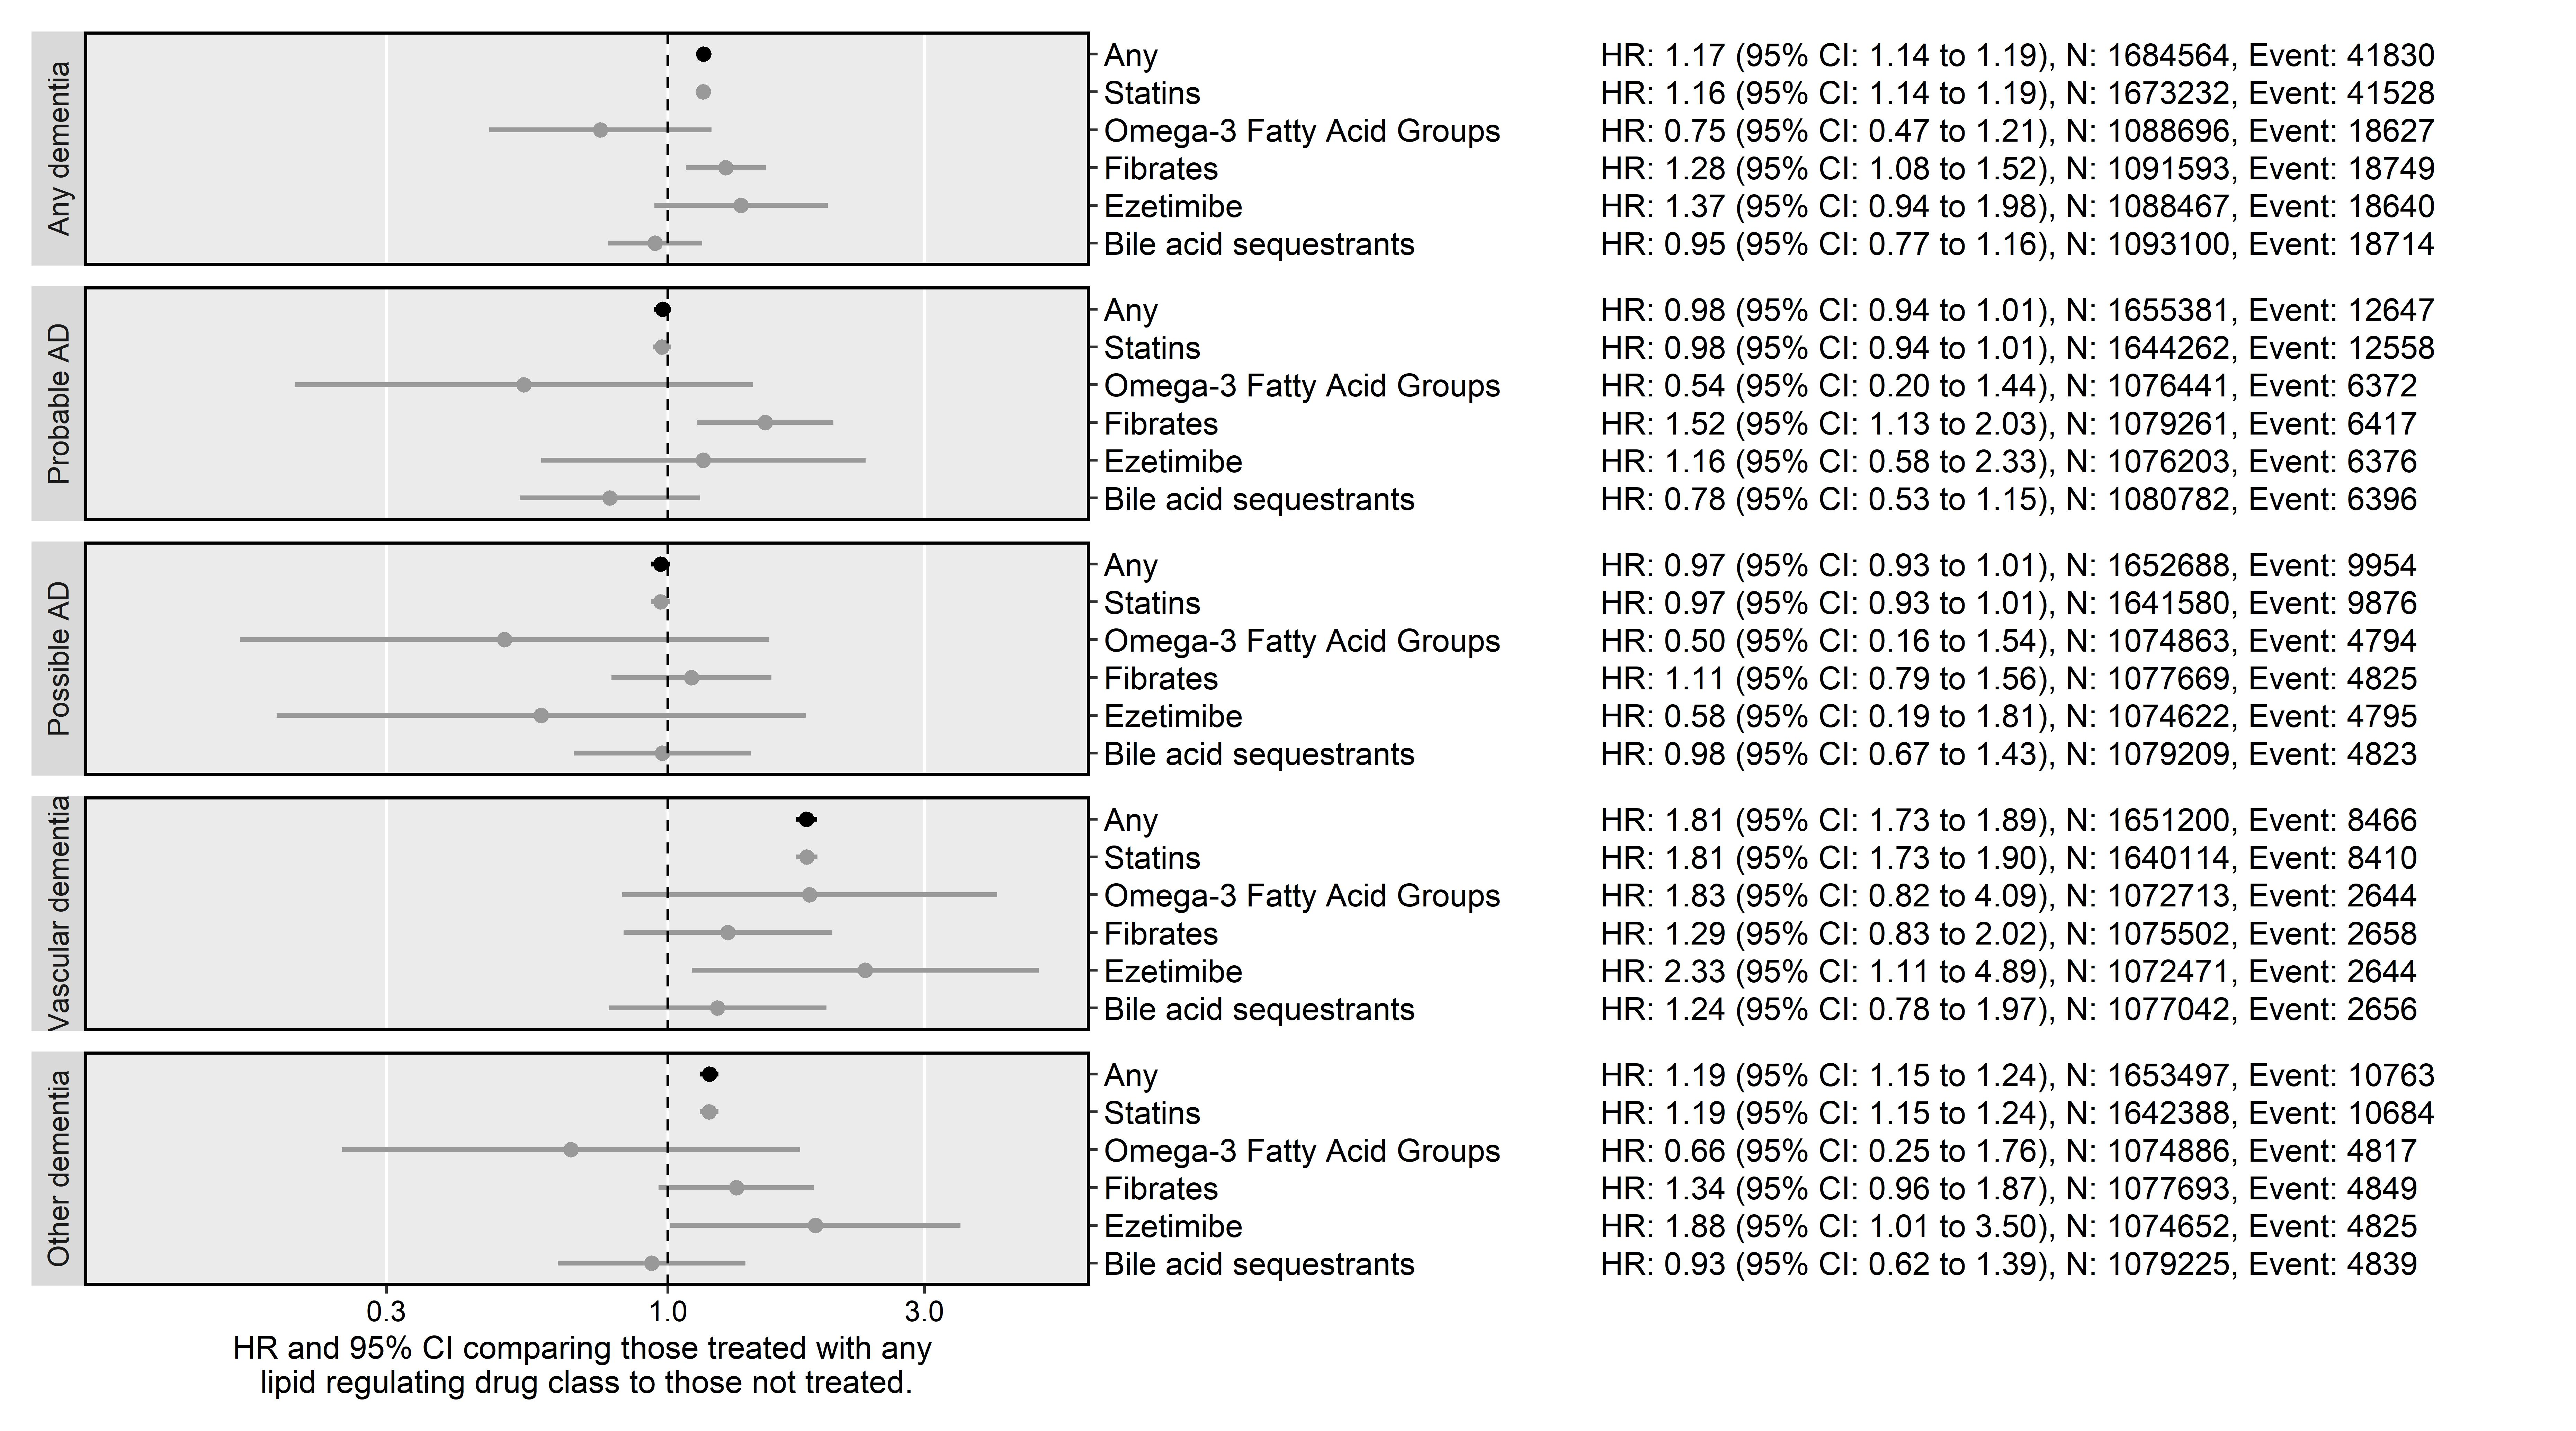
\includegraphics[width=1\linewidth]{figures/cprd-analysis/fp_p1} \caption[Results from primary analyses of CPRD data]{Results from primary analyses of CPRD data using the fully adjusted model and participant age as the time scale.}\label{fig:cprdPrimary}
\end{figure}

~

\textbf{Alzheimer's disease}

No evidence was found for an effect of lipid-regulating agents on probable (HR: 0.98, 95\%CI: 0.94-1.01) and possible (HR: 0.97, 95\%CI: 0.93-1.01) Alzheimer's disease when compared with no treatment, with the sole exception of fibrates on probable Alzheimer's disease (HR: 1.28, 95\%CI: 1.08-1.52).

~

\textbf{Non-Alzheimer's disease dementias}

In contrast to the findings for Alzheimer's disease outcomes, lipid-regulating agents were associated with an increased risk of a subsequent diagnosis of vascular dementia (HR: 1.81, 95\%CI: 1.73-1.89) or other dementia (HR: 1.19, 95\%CI: 1.15-1.24). Again this effect was driven mainly by the statin subgroup, but there was some evidence that ezetimibe was associated with an increased risk of vascular (HR: 2.33, 95\%CI: 1.11-4.89) and other (HR: 1.88, 95\%CI: 1.01-3.5) dementia.

~

\textbf{All-cause dementia}

For the composite all-cause dementia outcome, I found treatment with a lipid-regulating agent was associated with a slightly increased risk (HR: 1.17, 95\%CI: 1.14-1.19), but the magnitude of the association was not as extreme as that observed for the vascular dementia subgroup. There was also some evidence that fibrates were associated with increased risk of all-cause dementia (HR: 1.28, 95\%CI: 1.08-1.52).

~

\hypertarget{sensitivity-analyses-2}{%
\subsection{Sensitivity analyses}\label{sensitivity-analyses-2}}

The results of the series of sensitivity analyses performed are described in the following sections.

\hypertarget{complete-case-versus-imputed-data}{%
\subsubsection{Complete case versus imputed data}\label{complete-case-versus-imputed-data}}

In almost all cases, the use of imputed data resulted in a marginal attenuation of the effects observed when using a complete cases analysis. It should be noted that due to the large amount of missing data (e.g.~793,720 participants (46.8\%) were missing a baseline LDL cholesterol measure), the number of participants included in the complete case analysis was substantially smaller than that included when using imputed data. In this case, though the overall position of the effect estimates does not change substantially when using the imputed dataset, there is a noticeable gain in power.\textsuperscript{\protect\hyperlink{ref-sterne2009b}{200}}

~





\begin{figure}[H]
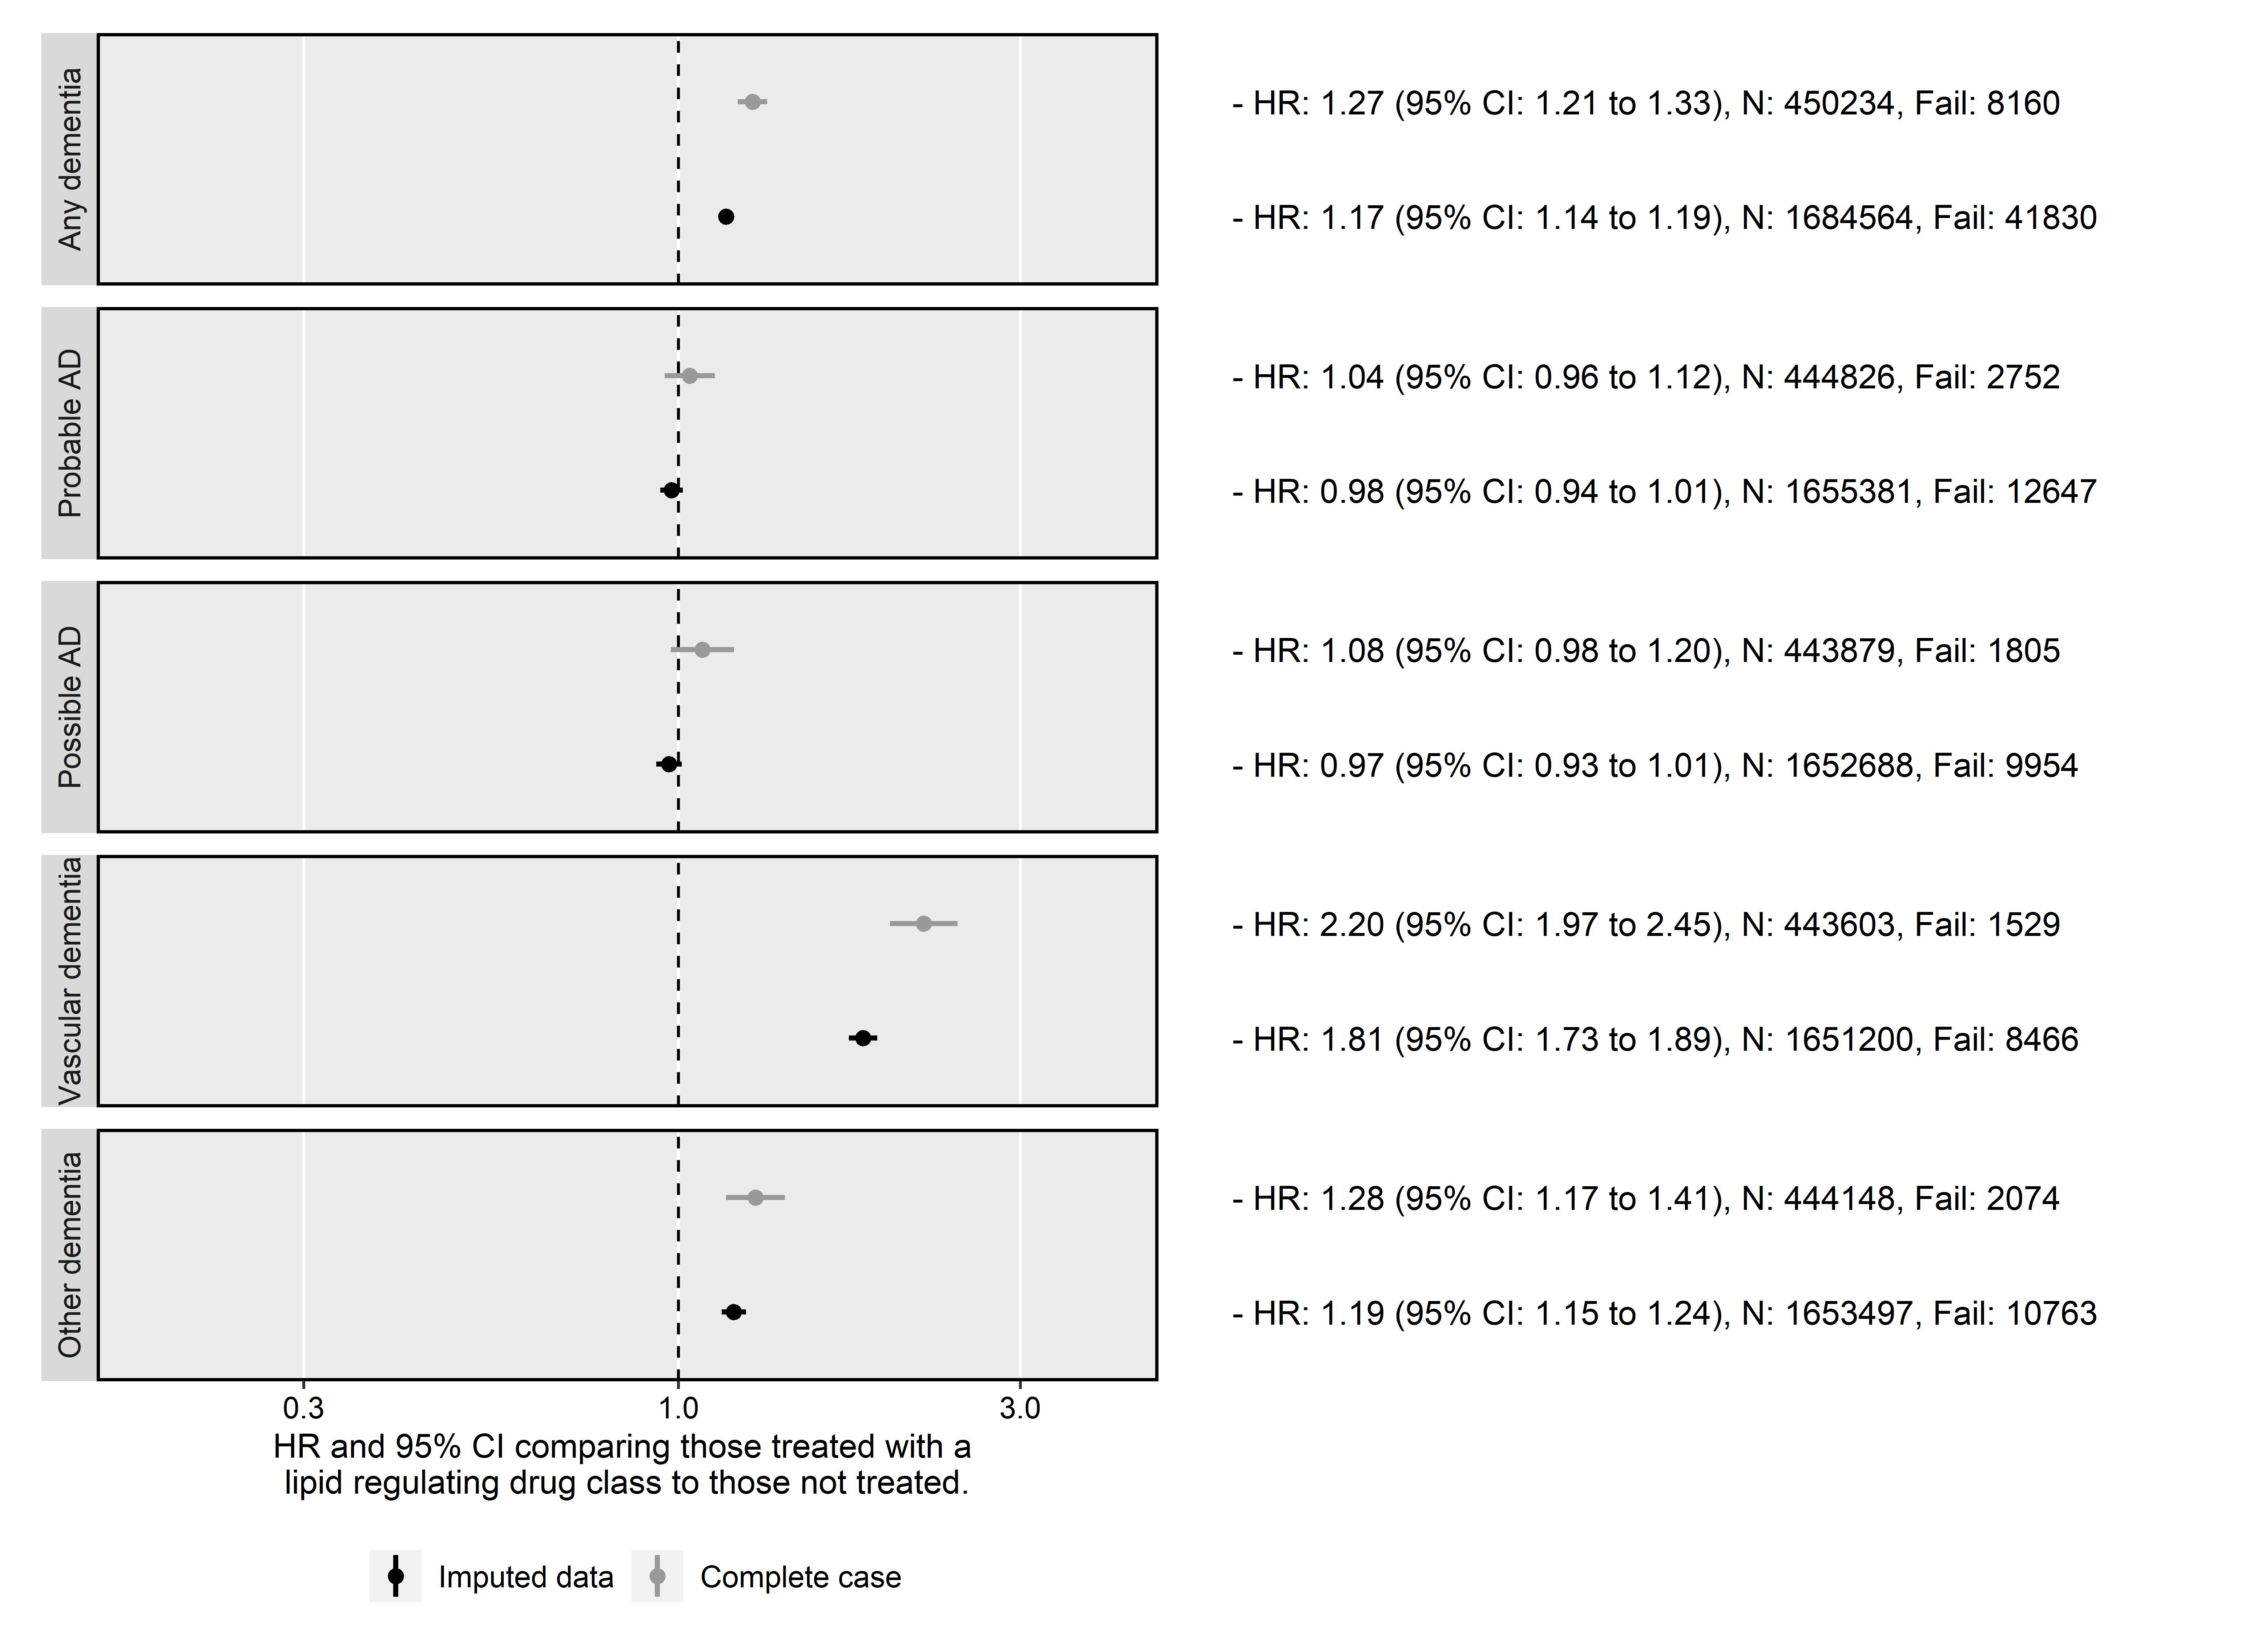
\includegraphics[width=1\linewidth]{figures/cprd-analysis/fp_complete_case} \caption[Complete case vs.~imputed data analysis]{Comparison of complete case versus imputed data analyses.}\label{fig:completeCaseFig}
\end{figure}

~

\hypertarget{control-outcomes-1}{%
\subsubsection{Control outcomes}\label{control-outcomes-1}}

Following the primary analysis, the fully adjusted model was used to estimate the effect of treatment with a statin on the two control outcomes of back pain (negative) and ischemic heart disease (positive). The results of this analysis are presented in Figure \ref{fig:controlOutcomeFig}.

For the negative control, there was some evidence that treatment with a statin was associated with an increased risk of back pain (HR: 1.04, 95\% CI: 1.03-1.05), suggesting there may be some residual confounding. However, statin prescription was also associated with a substantially increased risk of ischemic heart disease (HR: 1.62, 95\% CI: 1.59-1.64).

~





\begin{figure}[H]
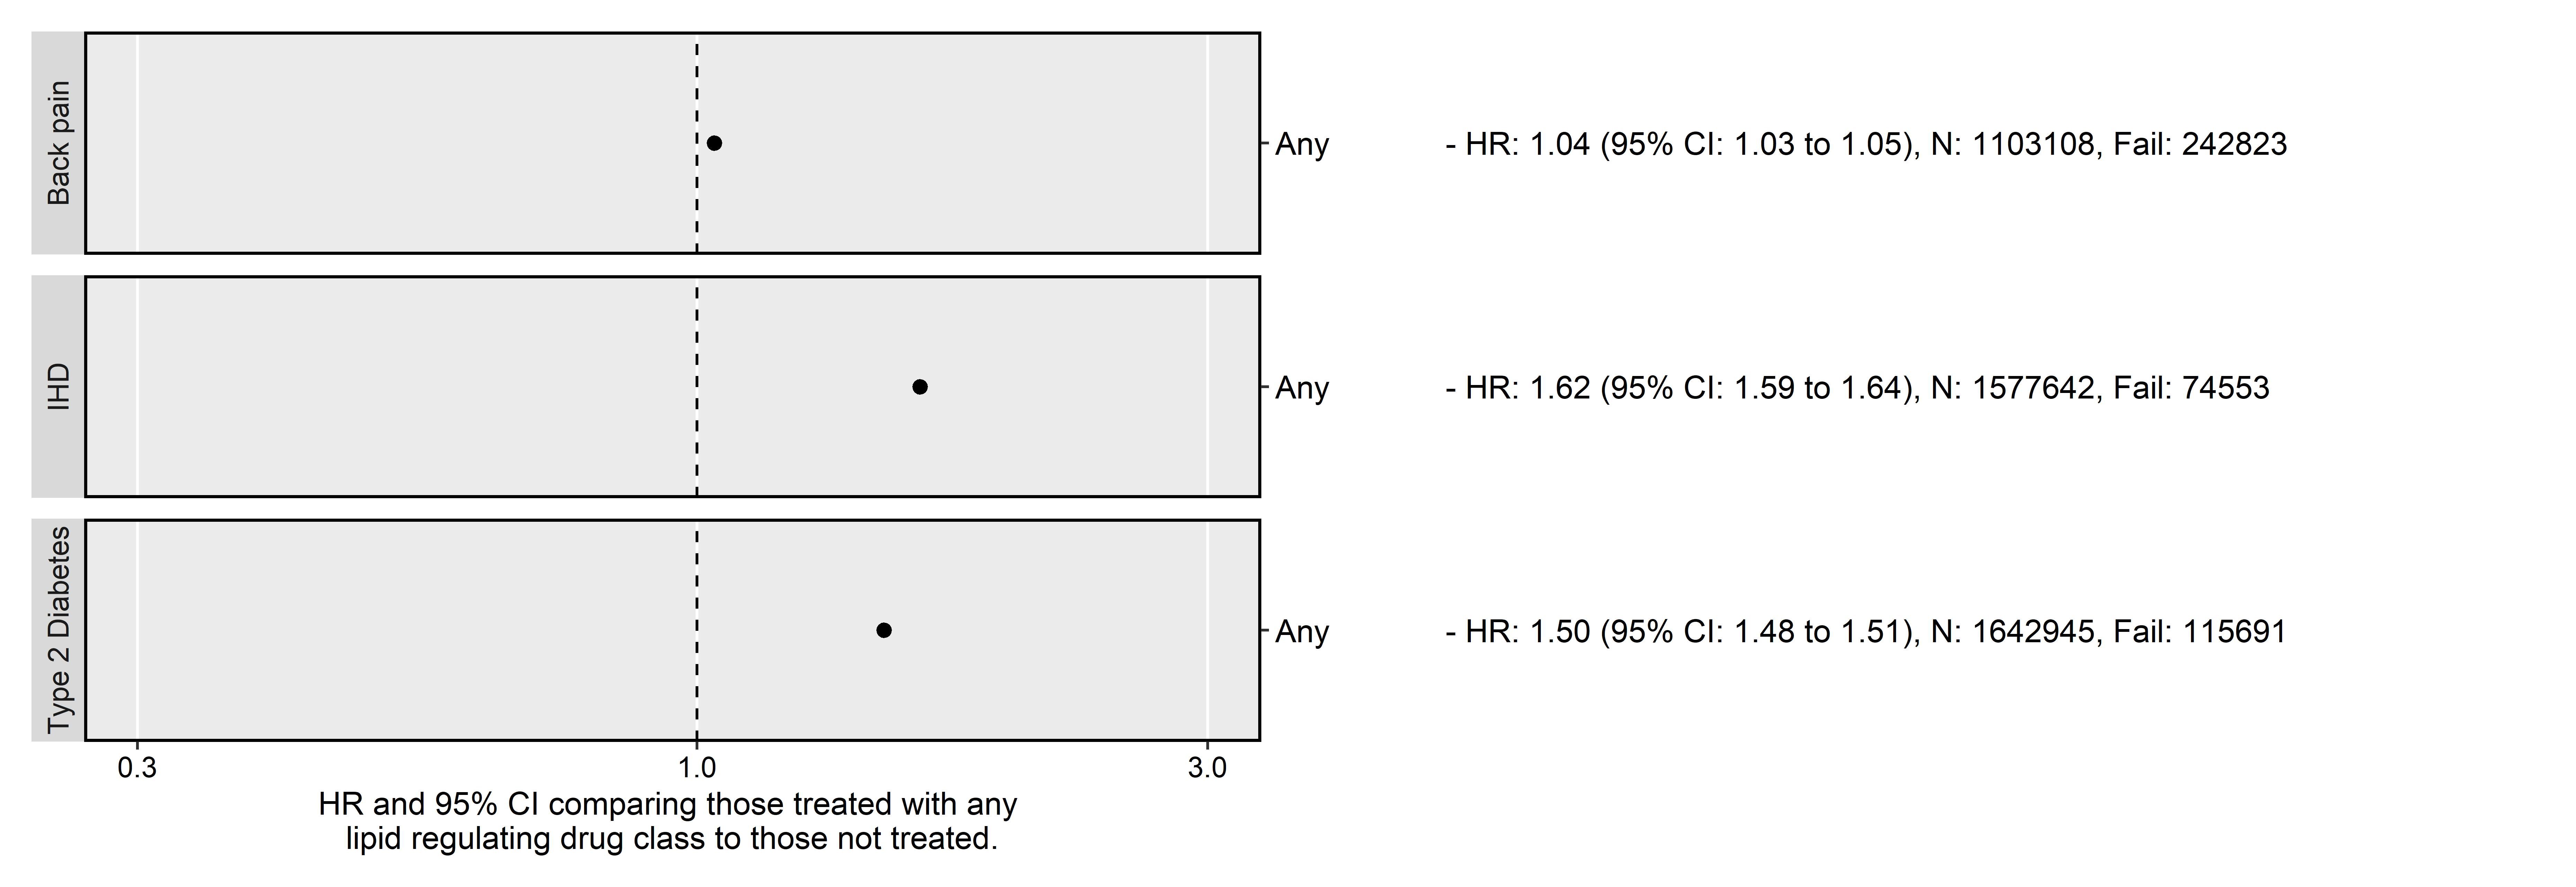
\includegraphics[width=1\linewidth]{figures/cprd-analysis/fp_control_outcomes} \caption[Results of control outcome analysis]{Results of control outcome analysis.}\label{fig:controlOutcomeFig}
\end{figure}

~

\hypertarget{impact-of-additional-covariates-1}{%
\subsubsection{Impact of additional covariates}\label{impact-of-additional-covariates-1}}

The results of three models adjusted for age only, age and sex, and the full covariates respectively, are presented in Figure \ref{fig:unadjustedComparisonFig}.

These models were used to estimate the impact of adjustment for additional covariates. Note that obtaining an completely unadjusted model is not possible, as age was used in the Cox model as the time scale.

Adjustment for additional covariates beyond age and sex had a limited impact on the observed effect estimates, with the exception of the Probable AD outcome. In this case, adjustment for the full set of covariates attenuated to the null the protective effect observed when adjusting only for age and sex.

~





\begin{figure}[H]
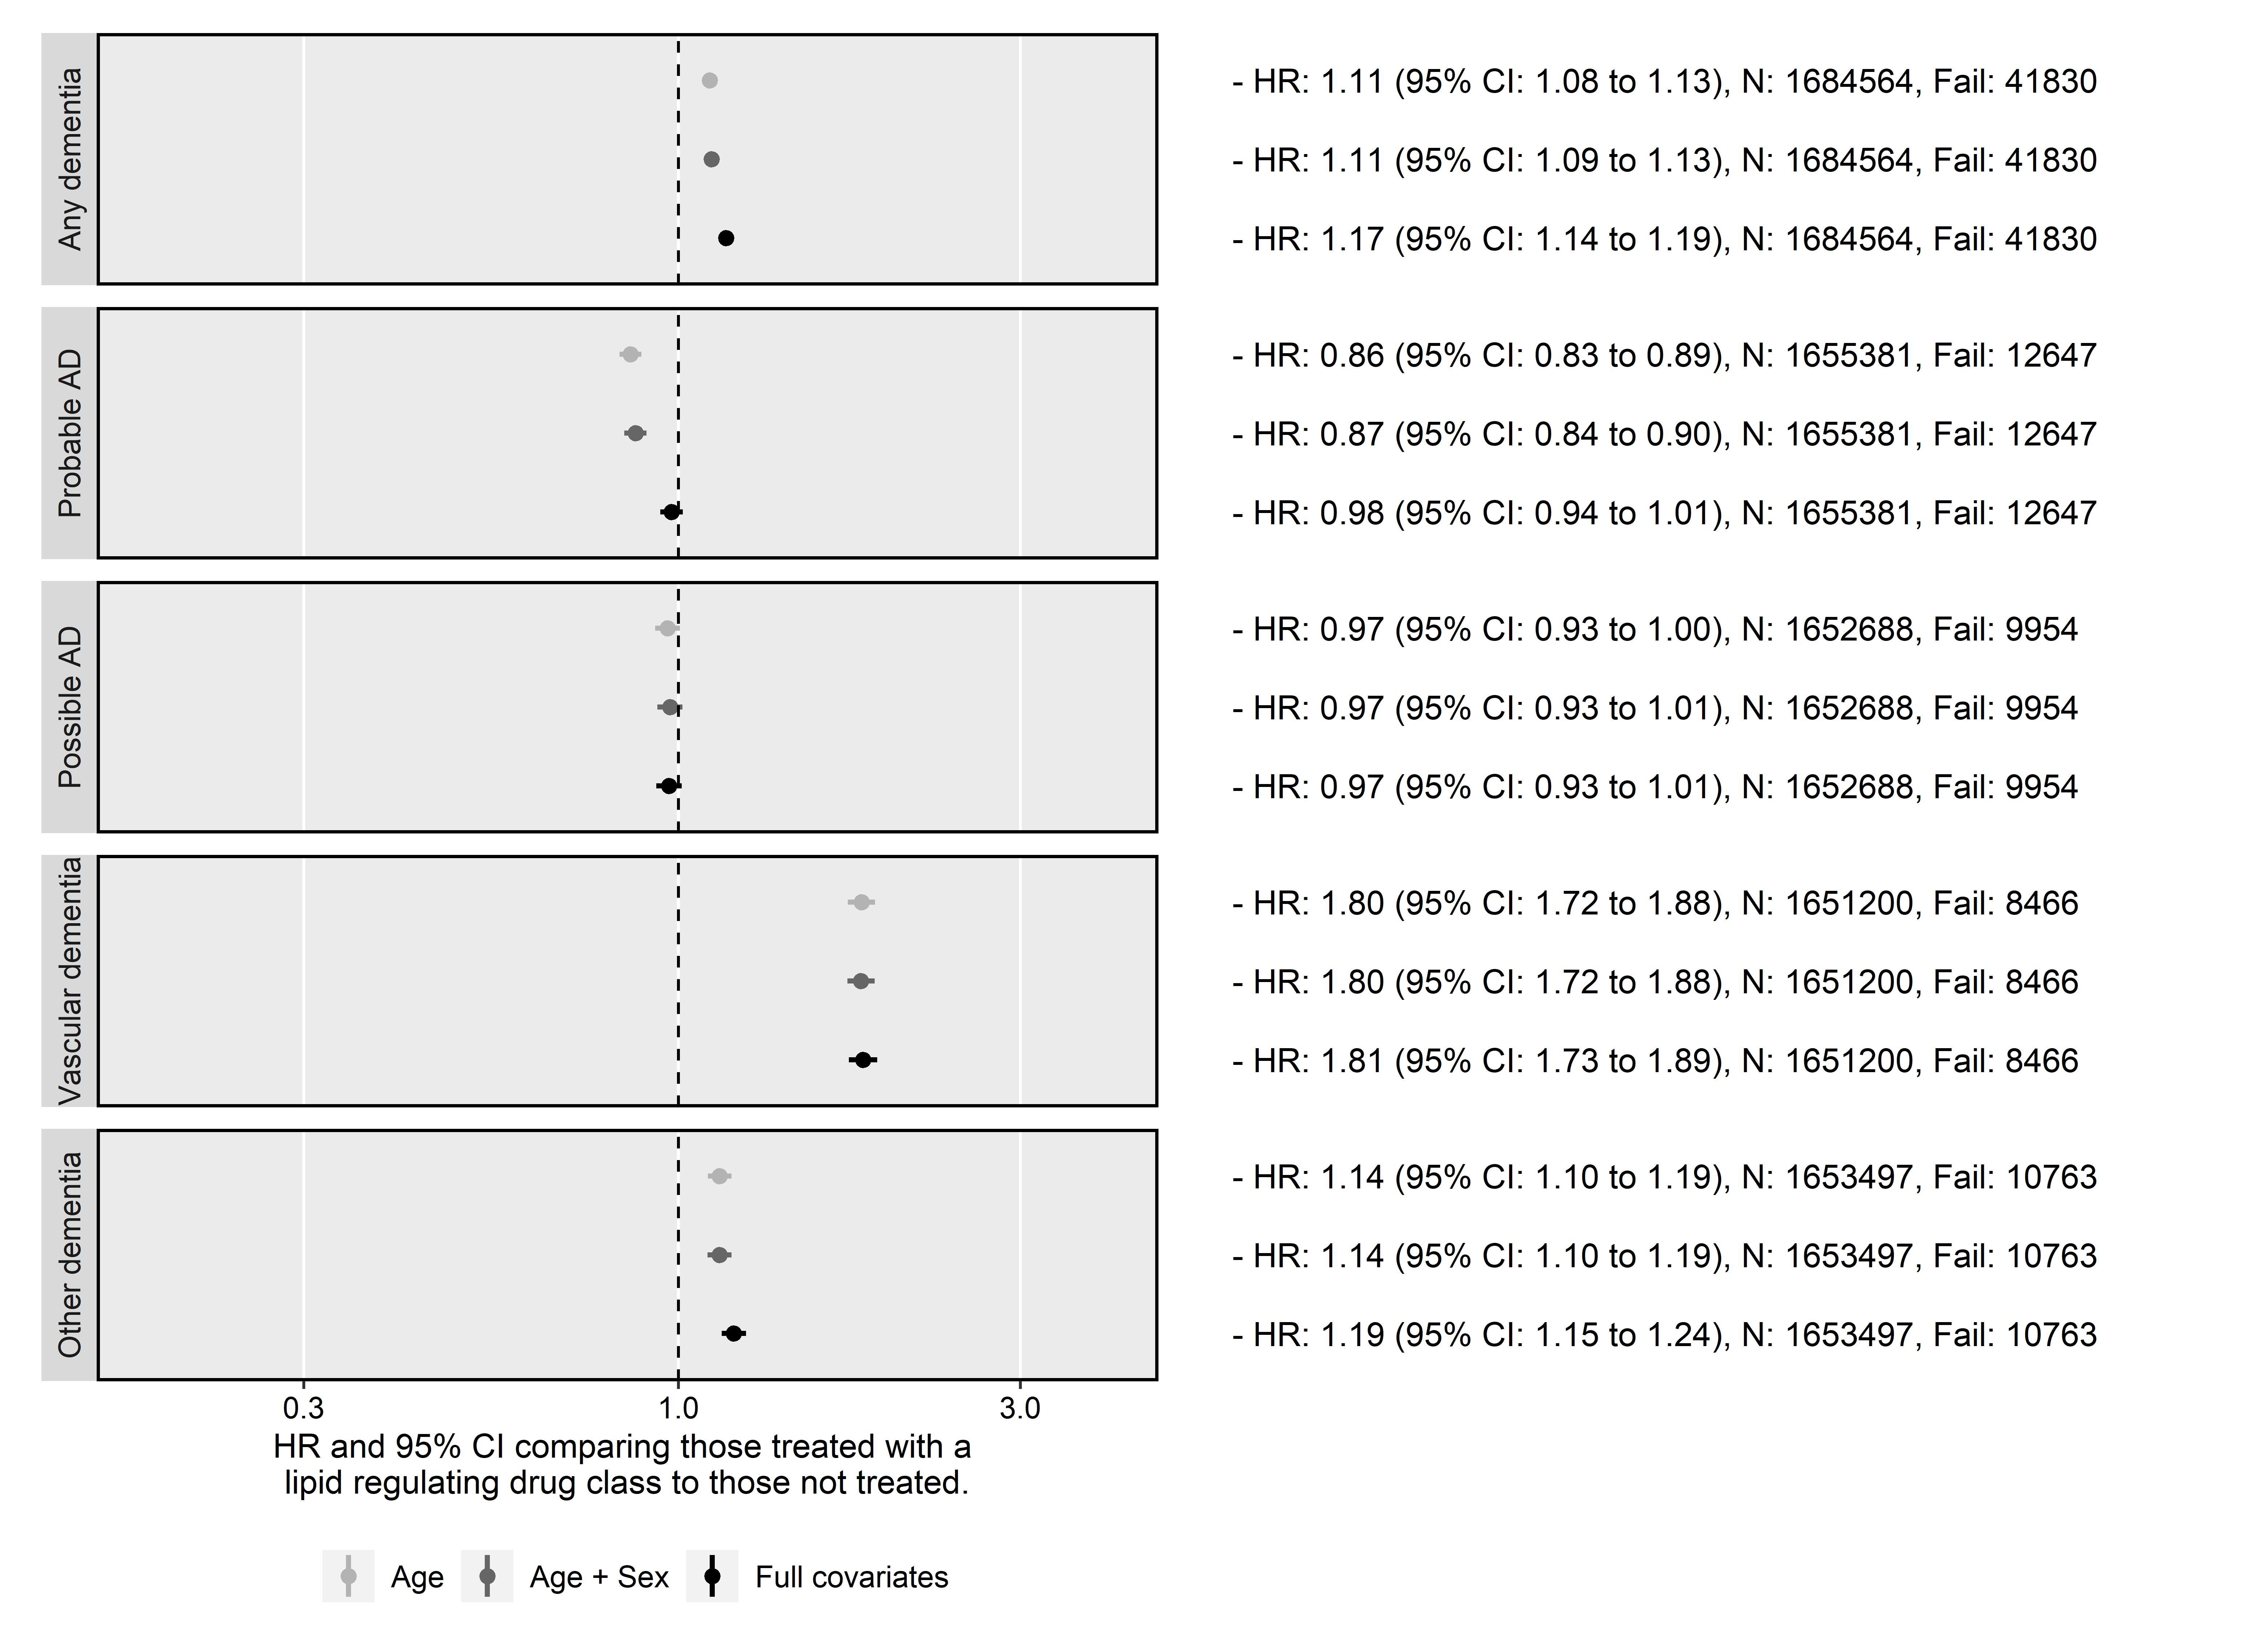
\includegraphics[width=1\linewidth]{figures/cprd-analysis/fp_unadjusted} \caption[Comparison of different combinations of covariates]{Results of three models adjusting for a different set of covariates.}\label{fig:unadjustedComparisonFig}
\end{figure}

\hypertarget{sensitivity-cohorts-entry-year}{%
\subsubsection{Sensitivity cohorts: Entry year}\label{sensitivity-cohorts-entry-year}}

When stratifying based on year of entry to the cohort, I observed no variation in risk by time period in any subgroup except for probable Alzheimer's disease (Figure \ref{fig:diagnosisTypeFig}).

~





\begin{figure}[H]
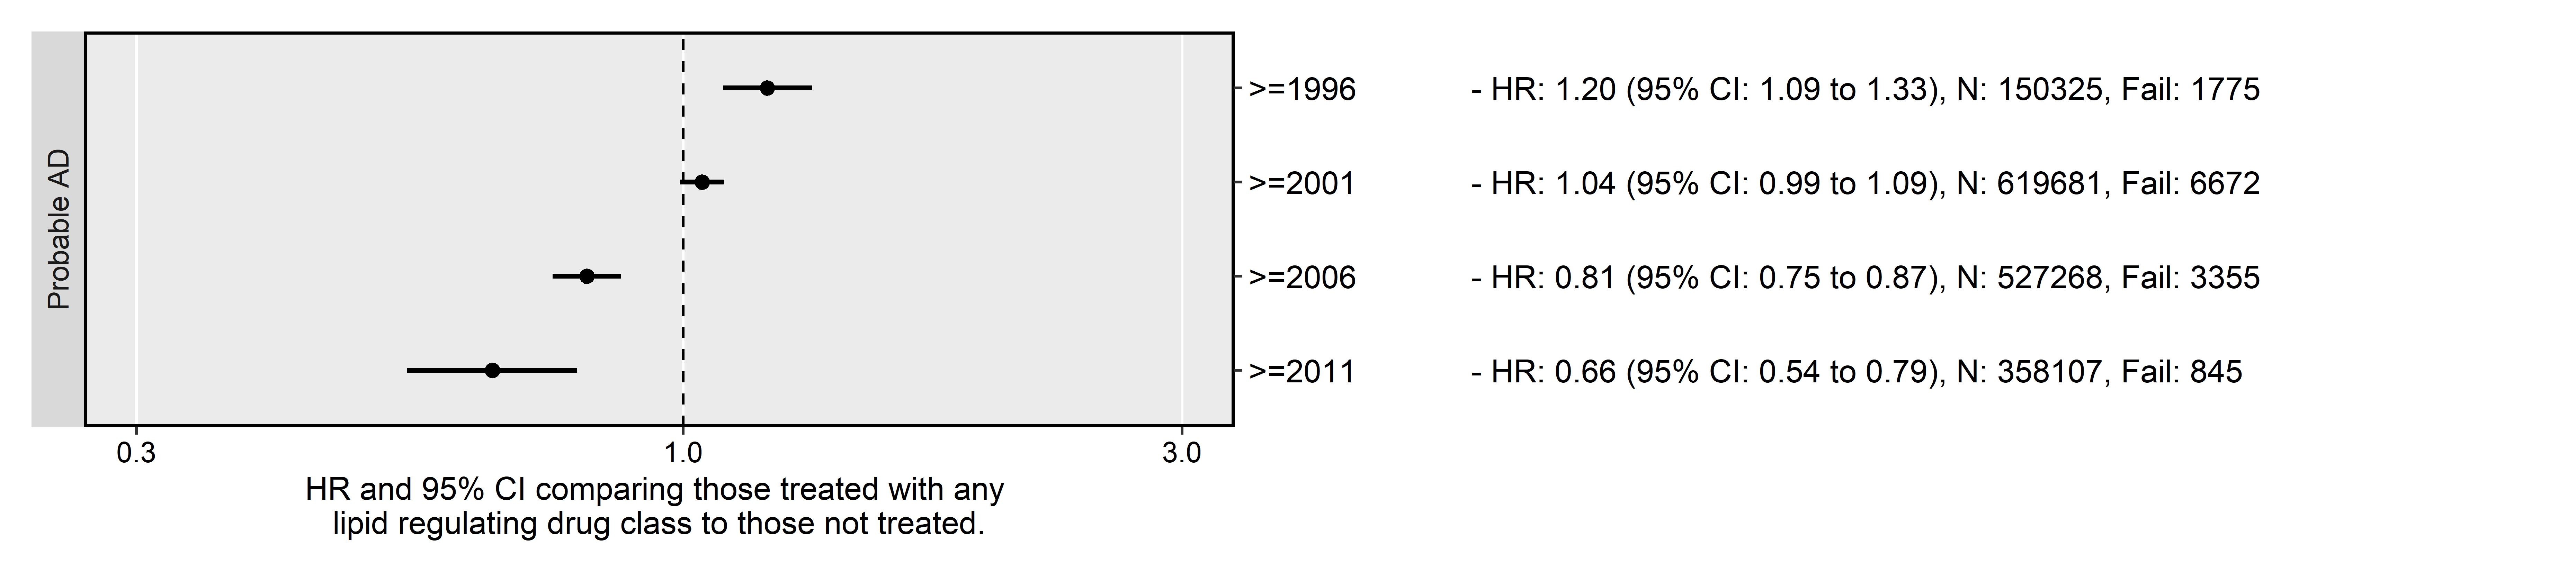
\includegraphics[width=1\linewidth]{figures/cprd-analysis/fp_cohort_entry} \caption[Sensitivty analus]{Analysis of any lipid regulating agent on Probable AD outcome, stratified by grouped year of cohort entry.}\label{fig:diagnosisTypeFig}
\end{figure}

~

On the assumption that this variation could be caused by changes in the frequency of codes used to define Probable AD in the cohort, I performed a \emph{post-hoc} investigation of the frequency of each diagnoses stratified by year of entry (Table \ref{tab:diagnosisType-table}). While the total frequency of any dementia outcome declines in more recent strata, likely due to the limited follow-up inherent to these groups, the decline in frequency is relatively constant across all dementia subtypes.

~





\begin{table}[H]

\caption[Frequency of diagnoses by grouped year of cohort entry]{\label{tab:diagnosisType-table}Frequency of diagnoses by grouped year of cohort entry}
\centering
\fontsize{7}{9}\selectfont
\begin{tabular}[t]{>{\raggedright\arraybackslash}p{5.33em}>{\centering\arraybackslash}p{5.33em}>{\centering\arraybackslash}p{5.33em}>{\centering\arraybackslash}p{5.33em}>{\centering\arraybackslash}p{5.33em}>{\centering\arraybackslash}p{5.33em}l}
\toprule
\textbf{\textbf{Year of cohort entry}} & \textbf{\textbf{No dementia}} & \textbf{\textbf{Probable AD}} & \textbf{\textbf{Possible AD}} & \textbf{\textbf{Vascular dementia}} & \textbf{\textbf{Other dementia}} & \textbf{\textbf{Total}}\\
\midrule
>=1996 & 148550 (95.9\%) & 1775 (1.1\%) & 1677 (1.1\%) & 1345 (0.9\%) & 1585 (1.0\%) & 154932\\
\midrule
>=2001 & 613009 (96.3\%) & 6672 (1.0\%) & 5711 (0.9\%) & 4857 (0.8\%) & 6073 (1.0\%) & 636322\\
\midrule
>=2006 & 523913 (98.1\%) & 3355 (0.6\%) & 2169 (0.4\%) & 1890 (0.4\%) & 2506 (0.5\%) & 533833\\
\midrule
>=2011 & 357262 (99.4\%) & 845 (0.2\%) & 397 (0.1\%) & 374 (0.1\%) & 599 (0.2\%) & 359477\\
\midrule
Total & 1642734 (97.5\%) & 12647 (0.8\%) & 9954 (0.6\%) & 8466 (0.5\%) & 10763 (0.6\%) & 1684564\\
\bottomrule
\end{tabular}
\end{table}

~

\hypertarget{sensitivity-cohorts-pregnancy}{%
\subsubsection{Sensitivity cohorts: Pregnancy}\label{sensitivity-cohorts-pregnancy}}

In the second sensitivity cohort, removing participants coded as female and aged 55 and under at index from the analysis had minimal effect on the effect estimates (Figure \ref{fig:pregnancyFig}).





\begin{figure}[H]
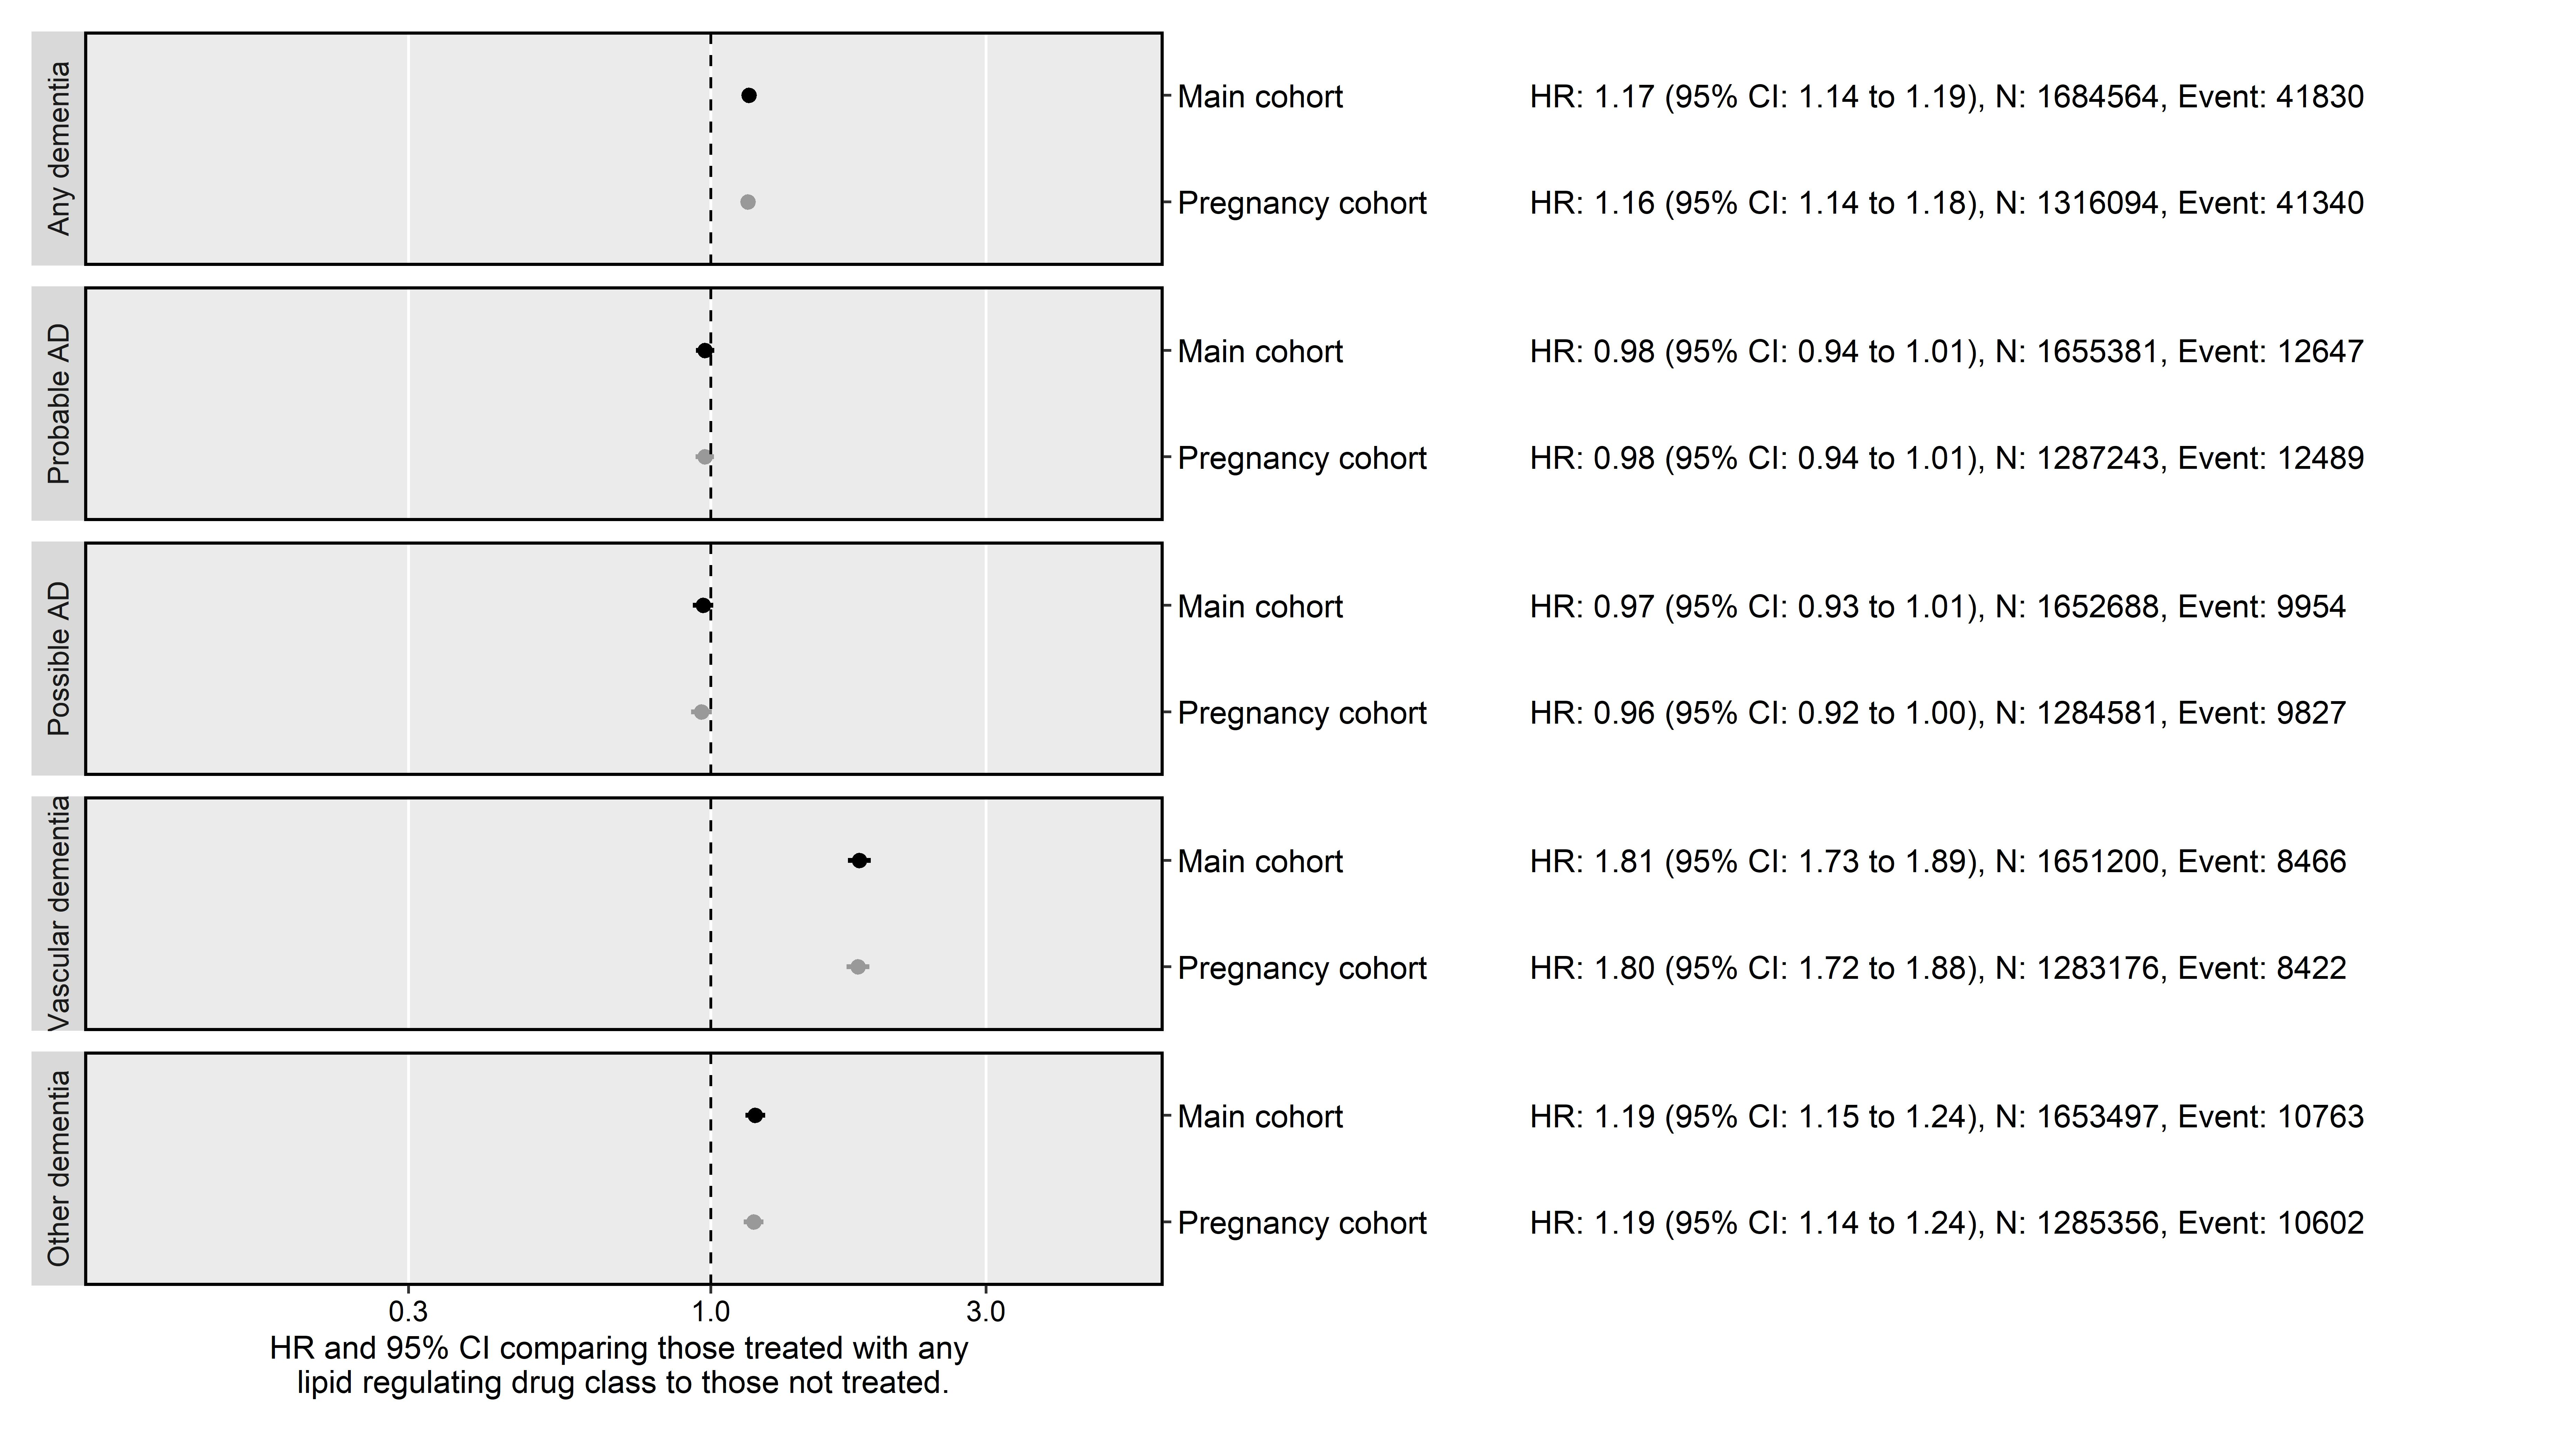
\includegraphics[width=1\linewidth]{figures/cprd-analysis/fp_pregnancy} \caption[Comparison of pregnancy analysis]{Comparison of analysis using main cohort and a cohort with potentially pregnany women removed.}\label{fig:pregnancyFig}
\end{figure}

~

\hypertarget{statin-properties-1}{%
\subsubsection{Statin properties}\label{statin-properties-1}}

In the cohort, statins with lipophilic properties were much more frequently prescribed than hydrophilic statins (Table \ref{tab:statinTypeTable-table}). Additionally, there is evidence for a increasing tendency to favour hydrophilic statins in recent years, as the proportion of lipophilic statins prescribed fell from 18.2\% in 1996-2000 to \textless1\% in 2011-2016.

~





\begin{table}[H]

\caption[Summary of statin properties (lipophilicity vs hydrophilicity).]{\label{tab:statinTypeTable-table}Summary of statin properties (lipophilicity vs hydrophilicity) by grouped year of prescription.}
\centering
\fontsize{7}{9}\selectfont
\begin{tabular}[t]{lccc}
\toprule
\textbf{\textbf{Prescription Year Group}} & \textbf{\textbf{Hydrophilic}} & \textbf{\textbf{Lipophilic}} & \textbf{\textbf{Total}}\\
\midrule
>=1996 & 7037 (18.2\%) & 31531 (81.8\%) & 38568\\
\midrule
>=2001 & 21427 (10.3\%) & 187018 (89.7\%) & 208445\\
\midrule
>=2006 & 3566 (1.6\%) & 217726 (98.4\%) & 221292\\
\midrule
>=2011 & 1115 (0.9\%) & 119035 (99.1\%) & 120150\\
\bottomrule
\end{tabular}
\end{table}

~

When stratifying by statin properties, hydrophilic statins were less harmful in the any, vascular and other dementia outcomes compared to lipophilic statins (Figure \ref{fig:statinTypeFig}). Additionally, in the AD outcomes, hydrophilic statins had a small protective effect, compared to the absence of evidence for an effect for lipophilic statins.

~





\begin{figure}[H]
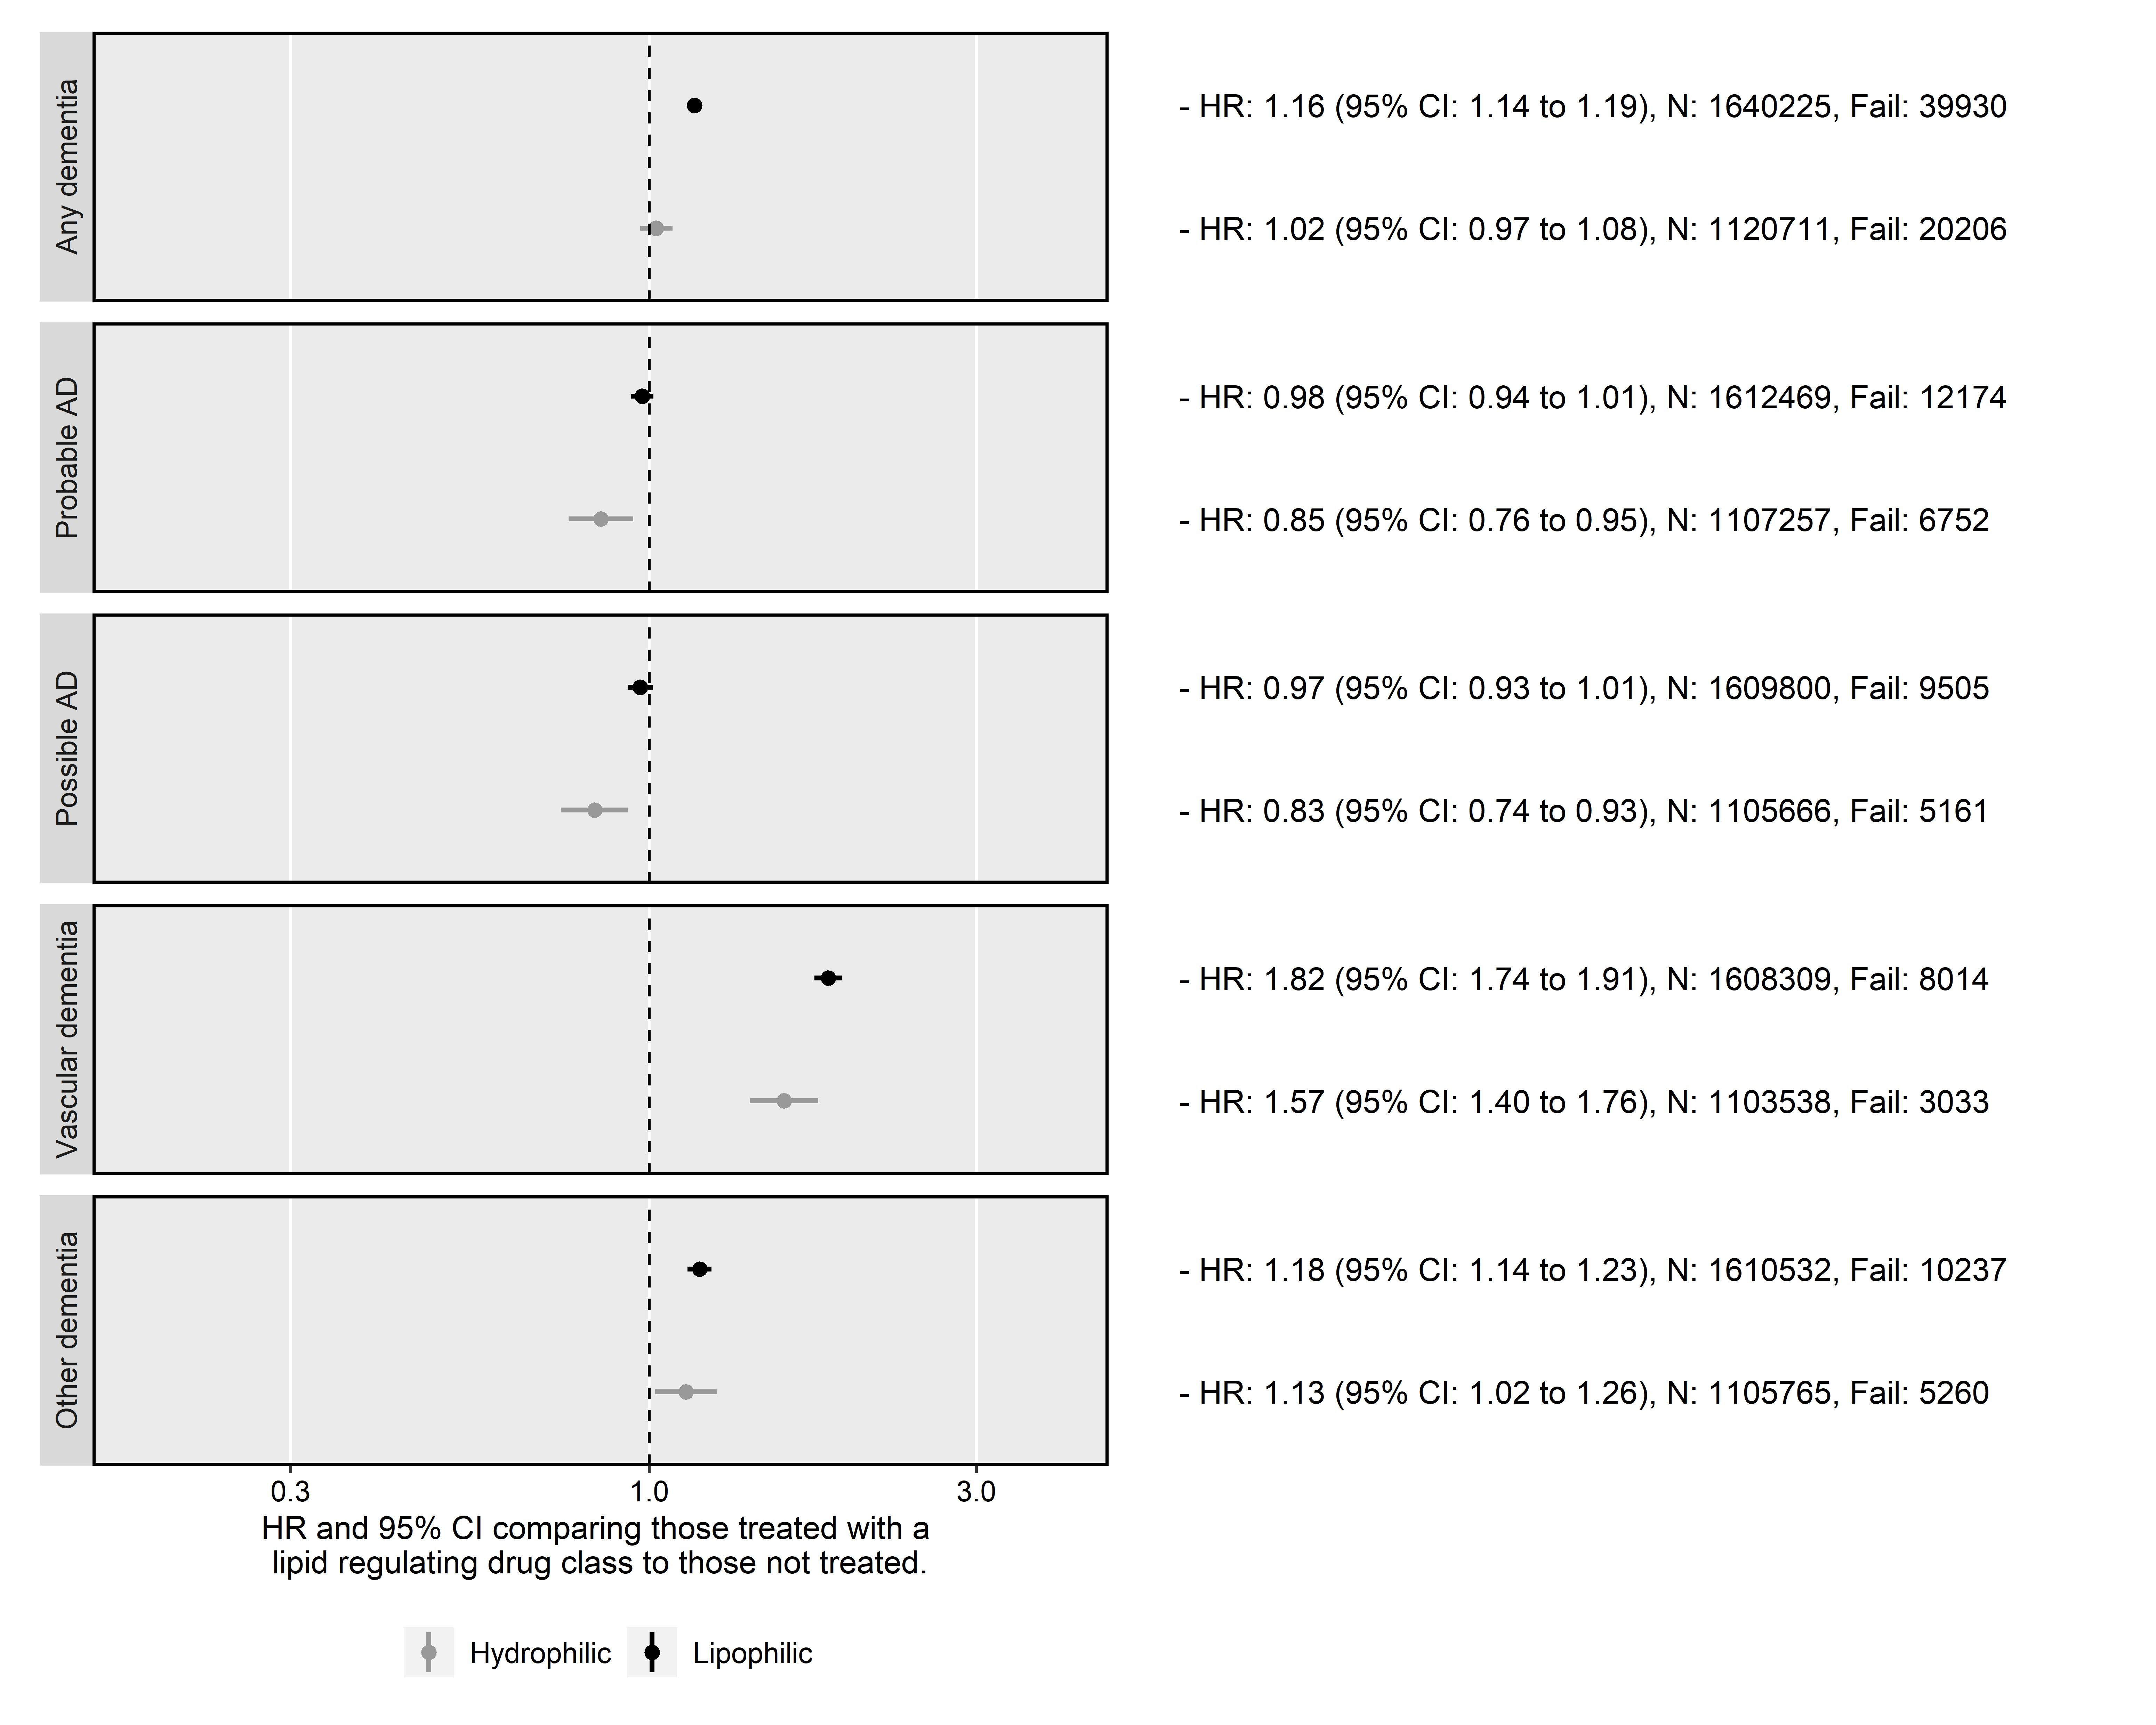
\includegraphics[width=1\linewidth]{figures/cprd-analysis/fp_sta_type} \caption[Analysis stratified by statin properties]{Analysis stratified by statin properties (hydrophilic vs lipophilic)}\label{fig:statinTypeFig}
\end{figure}

~

\hypertarget{comparing-codelists}{%
\subsubsection{Comparing codelists}\label{comparing-codelists}}

When using the Smeeth et al code lists to define dementia outcomes, effect estimates of HR: 1.19 (95\% CI: 1.07-1.32) and HR: 1.33 (95\% CI: 1.26-1.42) were obtained for the Alzheimer's disease and non-Alzheimer's dementia outcomes respectively.

However, comparison of the results using the two sets of code lists was deemed less useful following a comparison of the codes used. While all of the codes used to define Alzheimer's in the Smeeth paper are included in the Probable Alzheimer's code-list (see Figure \ref{fig:smeethComparison}), I included several additional codes used to define this outcome (including, for example, ``Eu00013: {[}X{]}AD disease type 2''). Additionally, several of the codes used to define ``Possible Alzheimer's'' in this analysis are included in the ``Other dementia'' code list used by Smeeth.

~





\begin{figure}[H]
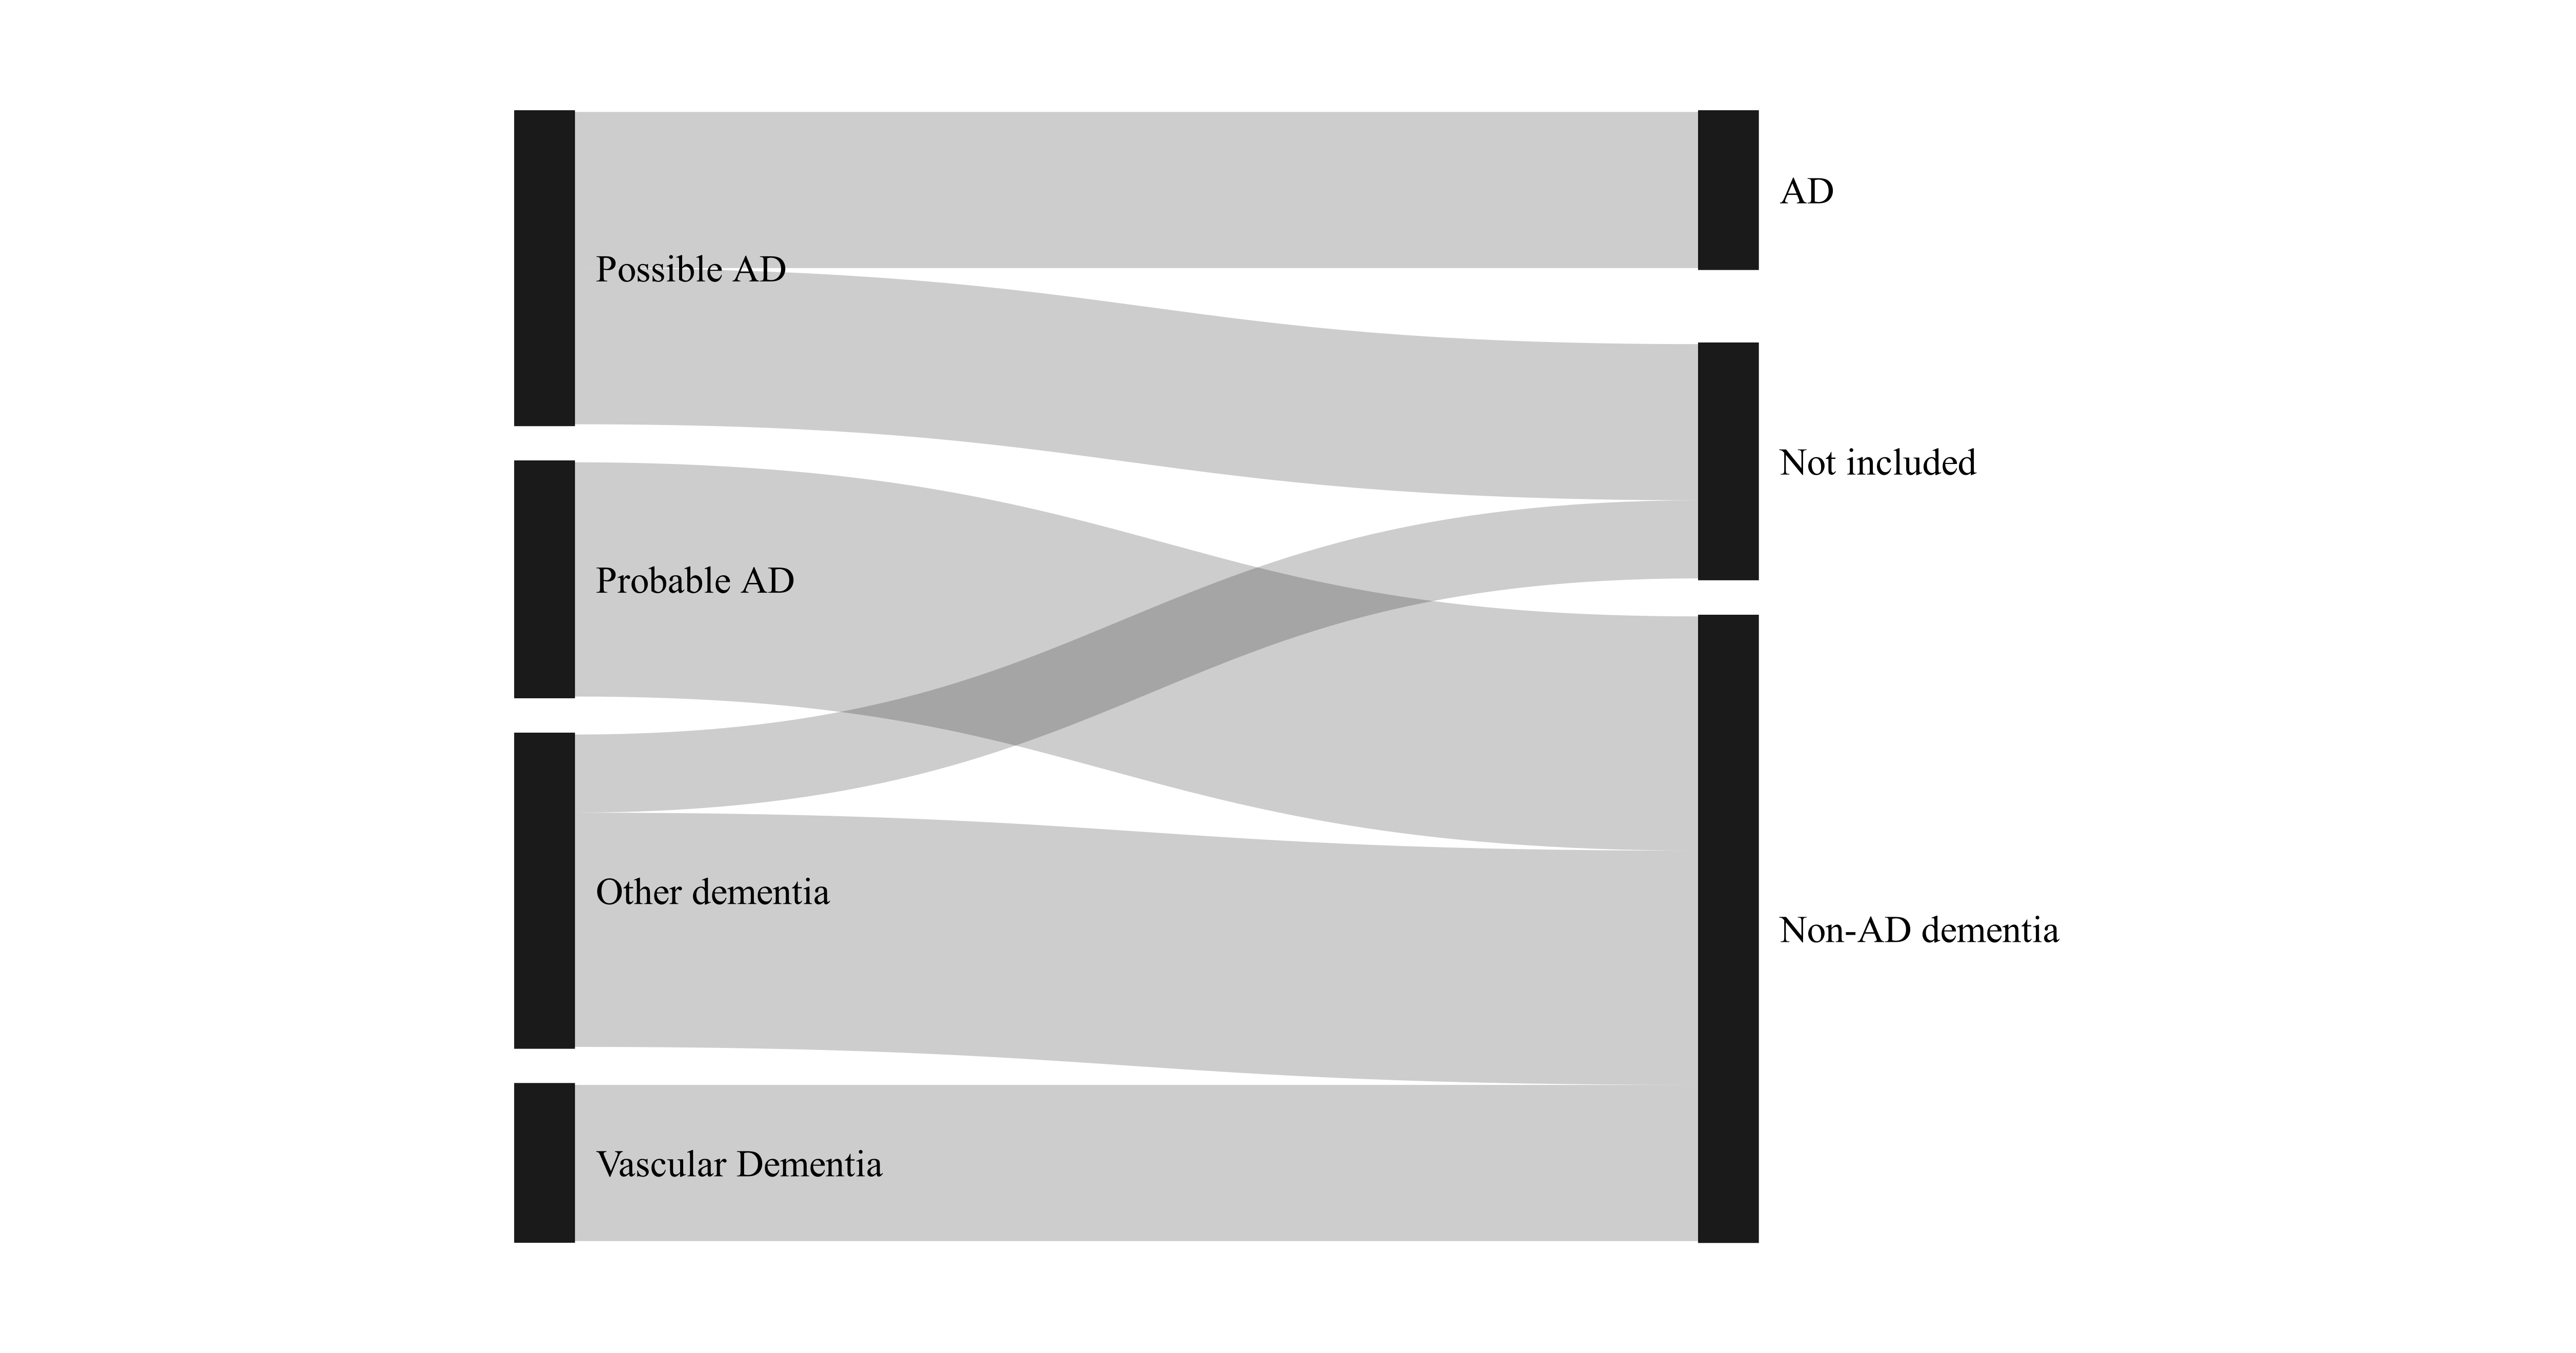
\includegraphics[width=1\linewidth]{figures/cprd-analysis/sankey_diagram} \caption[Comparison of code used in this analysis with those used in the Smeeth et al.~2010 paper]{Sankey diagram comparing the codes used in this analysis with those used in the Smeeth \emph{et al} paper.\textsuperscript{\protect\hyperlink{ref-smeeth2009}{199}} The outcomes and number of codes contributing to each are presented (the Smeeth \emph{et al} outcomes are on the right hand side of the figure). The joining lines showing the overlap between the categories in the two analyses.}\label{fig:smeethComparison}
\end{figure}

This analysis serves to illustrative the importance of the code lists chosen to define the outcomes of interest, particularly if they are competing (e.g.~AD vs non-AD dementia).

~

\hypertarget{discussion-2}{%
\section{Discussion}\label{discussion-2}}

\hypertarget{summary-of-findings}{%
\subsection{Summary of findings}\label{summary-of-findings}}

Lipid-regulating agents showed no evidence of an effect on probable and possible Alzheimer's disease when compared with no treatment, but were associated with increased risk of an all-cause dementia, vascular dementia and other dementia diagnosis. The effect observed in each case was driven by the statin subgroup, which included a substantial majority of participants. For the other drug classes, no association was found with any outcome, with two exceptions being that ezetimibe was associated with increased risk of vascular and other dementia, while fibrates were associated with increase risk of all-cause dementia and probable Alzheimer's disease.

The effect estimates were robust to the exclusion of potentially pregnant participants, and for all outcomes except Probable AD, no variation across grouped year of entry was observed. When looking at the statin subgroup alone, statin properties appeared to have a modifying effect, with hydrophilic statins being less harmful in the any, vascular and other dementia outcomes compared to lipophilic statins.

~

\hypertarget{interpretation-of-results}{%
\subsection{Interpretation of results}\label{interpretation-of-results}}

This section will expand on a potential explanation for the observed results detailed above. However, as the comparison of evidence across different sources is the aim of the triangulation exercise presented in later chapters, the section will not provide a detailed comparison with other published literature, except where needed to illustrate a methodological point. For a comparison of the result presented above with those from the systematic review (Chapter \ref{hold}) and the individual patient data analysis (Chapter \ref{hold}), see Section \ref{hold}.

A likely explanation for the observed increased risk of vascular and other dementia with lipid regulating agent use is residual confounding by indication. While the term has been used to describe different source of bias in epidemiological analyses,\textsuperscript{\protect\hyperlink{ref-salas1999}{201}} ``confounding by indication'' is used here to described the role of risk factors that both prompt treatment (in this case statins) and increase the risk of the outcome (in this case vascular dementia), thus causing a distorted positive association between the treatment and outcome (see Figure \ref{fig:indicationBias}). In causal inference language, statins and dementia are said to be d-connected as there is an open ``backdoor'' path between them via the uncontrolled confounders.\textsuperscript{\protect\hyperlink{ref-suttorp2015}{202}}





\begin{figure}[H]
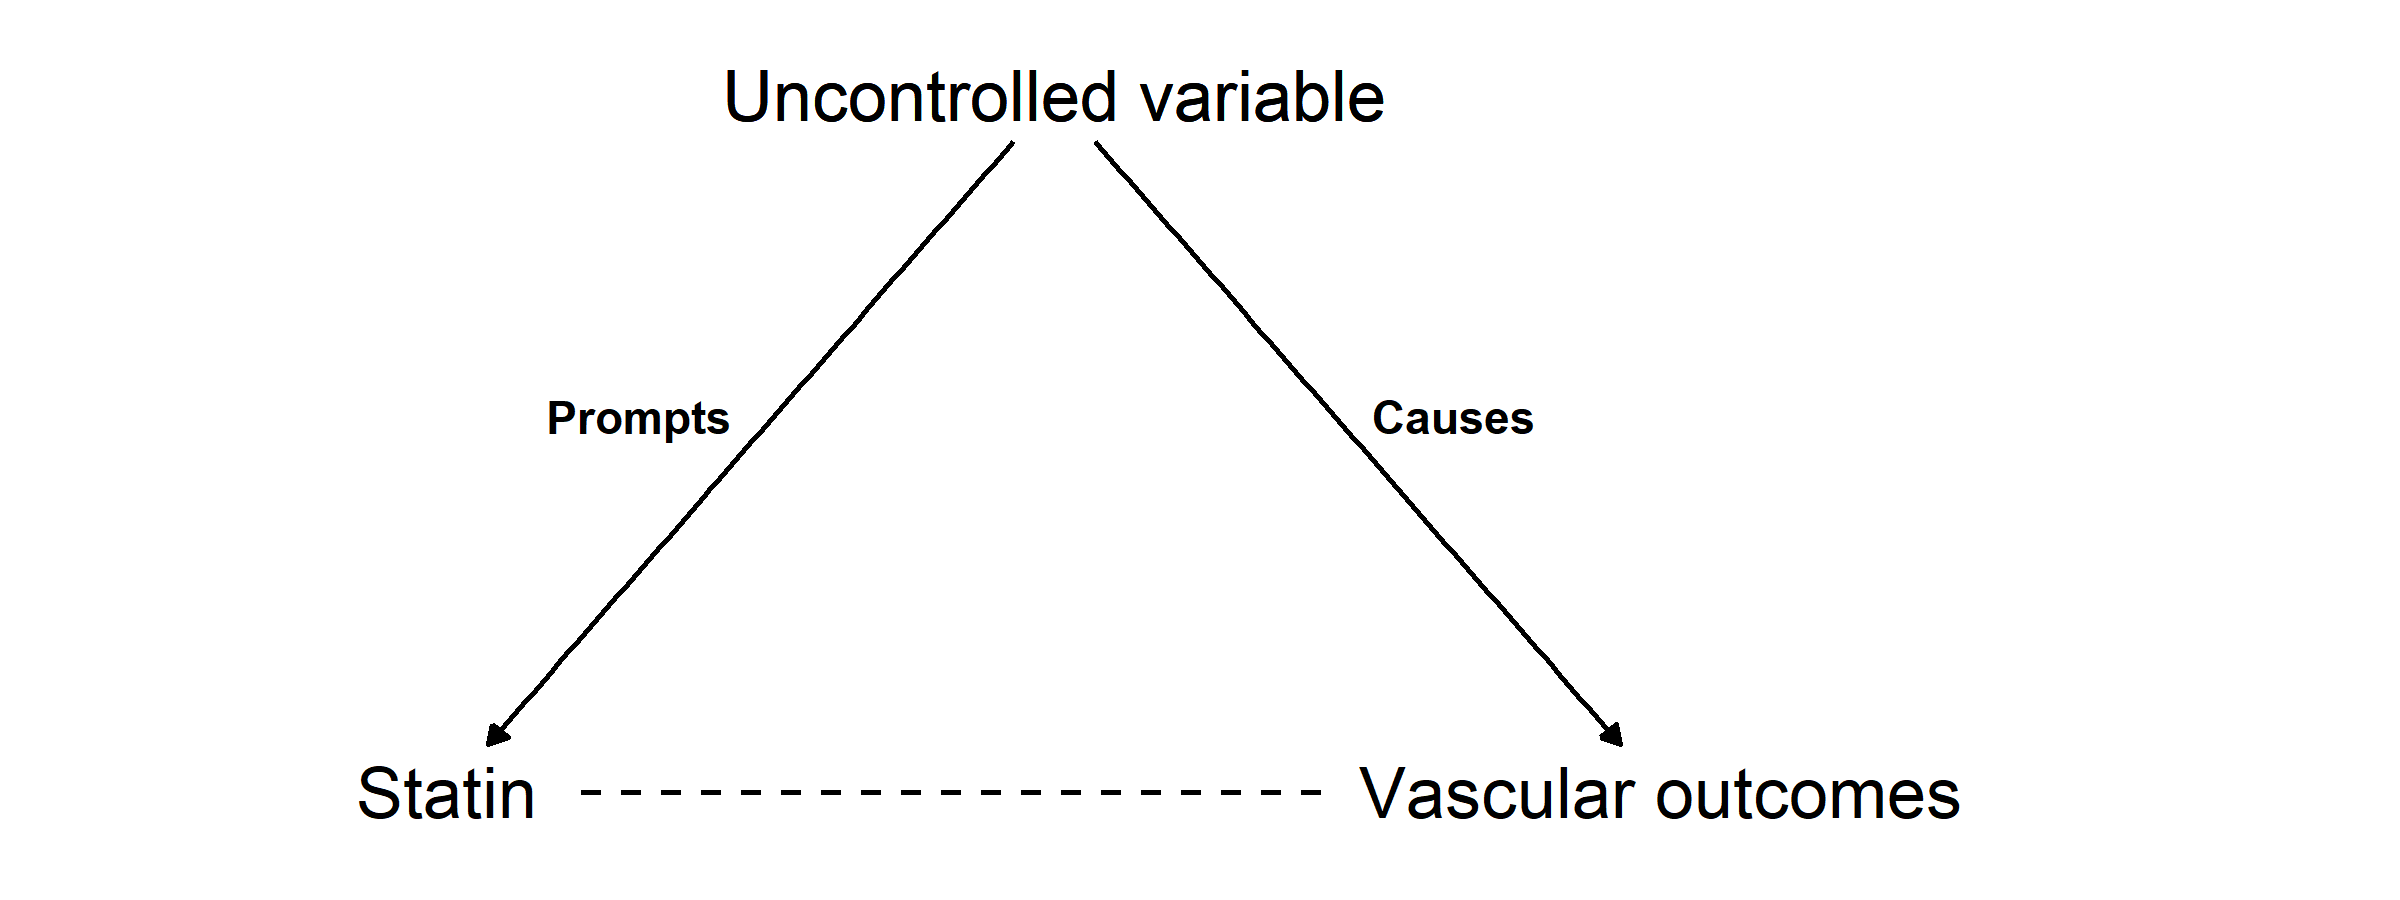
\includegraphics[width=1\linewidth]{figures/cprd-analysis/indicationBias} \caption[Confounding by indication causal diagram]{Causal diagram (directed acyclic graph) illustrating confounding by indication.}\label{fig:indicationBias}
\end{figure}

In the case of this analysis, the confounding variable (or, more likely, variables) would prompt prescription of statins (or another lipid regulating agent) but also represent a vascular risk factor that contributes to the development of the vascular dementia.

Supporting evidence for this interpretation comes from a variety of sources, including the results of the control outcome analyses. The slight harmful effect for the backpain outcome is substantially smaller that that observed for the ischemic heart disease outcome, indicating that the majority of the uncontrolled confounding is likely related to vascular factors. This is supported by the increasingly harmful effect moving from Probable/Possible AD to other dementia to vascular dementia, indicating that the confounding by indication likely increases as the proportion of vascular outcomes increase. This is supported by the decision tree for assigning outcomes in the presence of greater than one dementia code, where the Alzheimer's disease outcomes require a ``pure'' condition, and the presence of any vascular or other dementia codes excludes participants from this group (Figure \ref{fig:decisionTreeFig}).

A review of other available literature suggests that this observation (a harmful effect of lipid regulating agents on vascular-related outcome) is not unusual. Using a conventional epidemiological technique, a previous analysis also found an increased risk of coronary heart disease (analogous to ischemic heart disease) in those taking statins (HR: 1.31, 95\% CI: 1.04-1.66).\textsuperscript{\protect\hyperlink{ref-danaei2013b}{203}} Following control for confounding by indication through use of a trial emulation analysis, the expected protective effect of statins was observed.

Conditioning entry into the study on being either ``at-risk'' or already diagnosed with hypercholesterolemia was employed in a pre-emptive attempt to mitigate confounding by indication, but evidence from the control outcomes suggests this was unsuccessful. I also adjusted for several additional potential baseline variables. However, important confounding variables for which I have not adjusted could include genetic factors. A recent preprint of a study in the UK Biobank demonstrated that an Alzheimer's disease polygenic risk score was associated with an increased risk of vascular dementia, and also with an increased frequency of self-reported raised cholesterol levels, a diagnosis of hypercholesterolaemia, and a history of taking lipid-regulating agents such as statins or ezetimibe.\textsuperscript{\protect\hyperlink{ref-korologou-linden2020}{204}}

On a more general note, the unexpected increase in vascular dementia risk with statin use is particularly interesting given the absence of vascular dementia in the published literature, as highlighted in the previous chapter (see Section \ref{sys-rev-pub-bias}). It is possible that previous research identified a similar effect to this analysis, and via a publication bias mechanism, these results did not make it into the evidence base.

In summary, despite best efforts to account for strong confounding, participants prescribed a lipid regulating agent likely have a different vascular risk profile that those who are not, which may induce a spurious harmful association between lipid regulating agent use and vascular dementia outcomes.

~

\hypertarget{strengths-and-limitations}{%
\subsection{Strengths and limitations}\label{strengths-and-limitations}}

The primary strength of this analysis compared to others available in the literature is the relative size of the CPRD and length of follow-up. Having reviewed the other studies identified by the systematic review in Chapter \ref{sys-rev-heading}, this analysis of 1,684,564 participants is one of the largest available studies of this research question. Additionally, this analysis followed LRA users and non-users from a common index date, using a time-updating treatment indicator to correctly assign time-at-risk to the exposed and unexposed groups. This approach has been less commonly used in the literature and allows for the mitigation of potential immortal time bias.

However, the findings of this analysis are subject to several limitations. There is a strong possibility of differential misclassification\textsuperscript{\protect\hyperlink{ref-porta2014dictionary}{205}} of dementia-related conditions based on the exposure. As an illustrative example, those with memory complaints may be more likely to be classified as vascular dementia than Alzheimer's disease if their medical records contains prescriptions for lipid-regulating agents. Further, there is a potential for general non-differential misclassification of the outcome based on varying positive predictive value of electronic health record code lists to identify dementia cases.\textsuperscript{\protect\hyperlink{ref-wilkinson2018}{206},\protect\hyperlink{ref-mcguinness2019b}{207}}

Misclassification of outcomes is not the only issue introduced by the use of EHR codes to define outcomes. Comparing and contrasting between different studies is particularly difficult because of the impact that the use of different code list can have on the analysis. This is a particular challenge in comparing research across different time-periods and coding systems, as illustrated by the discrepancy between the results when using the codes lists defined for this study and those used by Smeeth \emph{et al}.

~

\hypertarget{cprd-data-avail}{%
\subsection{Enabling easy synthesis of this analysis}\label{cprd-data-avail}}

In light of my own experiences in attempting to extract information for papers assessing preventative treatments, as documented in Section \ref{sys-rev-open-data}, the outputs from this analysis are readily available.

All code, Read codelists and summary statistics (i.e.~the tables presented in this chapter, plus summary tables of effect estimates) are readily available in machine readable formats (i.e.~as comma separated values, or CSV, files) from the archived repository for this project (Zotero DOI: XXXX-XXXX).

The raw data supporting this analysis is not available, as access to the CPRD data is controlled by a data monitoring committee. In the context of access-controlled data, sharing the analysis code represents a way for readers to validate the findings.\textsuperscript{\protect\hyperlink{ref-goldacre2019c}{208}}

Additionally, to help ensure accurate reporting of this analysis, the Strengthening the Reporting of Observational Studies in Epidemiology (STROBE) reporting guidelines were used\textsuperscript{\protect\hyperlink{ref-vandenbroucke2007}{209}} (see Appendix \ref{hold} for the STROBE checklist).

This open approach will enable easy inclusion of this analysis in future evidence synthesis exercises, allowing new work to readily build on that presented here.

~

\hypertarget{conclusions}{%
\subsection{Conclusions}\label{conclusions}}

This chapter has provided new evidence on the potential repurposing of lipid-regulating agents for the prevention of all-cause dementia, Alzheimer's disease, vascular dementia, and other dementia. It made use of a large scale electronic health record database, the CPRD, and employed a time-varying Cox proportional hazards model to account for the potential immortal time bias.

It found no evidence for an effect of lipid-regulating agents on probable or possible Alzheimer's disease. However, lipid regulating agent use was associated with an increased risk of all-cause, vascular and other dementias. In all cases, the estimated associations were driven by those observed in the statin subgroup, which comprised the majority of exposed participants in this cohort.

This chapter attempted to account for important sources of bias and provide a comparison with other available literature, as identified in the systematic review presented in Chapter \ref{sys-rev-heading}. However, there is a strong potential for uncontrolled confounding by indication and differential misclassification of the outcome on the basis of exposure, which raises questions about the findings, in particular the unexpected increase in risk of vascular dementia associated with statin use. This is supported by our findings for the negative and positive control outcomes used, which provide some evidence of uncontrolled vascular confounders that may both prompt LRA prescription and increase risk of vascular dementia. Future research using large scale electronic health records should aim to address these limitations, potentially by using a analytical design that more closely emulates a trial.\textsuperscript{\protect\hyperlink{ref-danaei2013b}{203}}

Regardless, this analysis has provided an additional source of evidence for the triangulation exercise presented in Chapter \ref{discussion-heading}. In the following Chapter, the dataset described here is incorporated along with several other datasets as part of an IPD analysis to investigate the effect of blood lipid levels on dementia outcomes directly, rather than via the proxy of treatment.

\newpage

\hypertarget{references-3}{%
\section{References}\label{references-3}}

--- Hold --- Hold

\hypertarget{ipd-heading}{%
\chapter{Individual participant data meta-analysis}\label{ipd-heading}}

\minitoc 

\hypertarget{lay-summary-4}{%
\section{Lay Summary}\label{lay-summary-4}}

\hypertarget{introduction-2}{%
\section{Introduction}\label{introduction-2}}

Is there a good way to visualise input of cohorts into an IPD analysis?

\hypertarget{methods-2}{%
\section{Methods}\label{methods-2}}

As part of the IPD analysis, relevant cohort studies were identified from the sty and approached. In the first instance, the corresponding author on the main man

Talk about how different covariates were managed across cohorts,

Talk about missing data was handled

\hypertarget{data-sources}{%
\subsection{Data sources}\label{data-sources}}

Several cohort studies were approach

As part of this Chapter, I will use individual patient data from a range of sources. These sources are described here in detail for reference.

Should also include a list of reasons why specific additional cohorts were not included - some like the EHR might be too big to get

Each should have:

\begin{itemize}
\tightlist
\item
  Description (including observation period, numbers, numbers with outcome, etc)
\item
  Whether they are a known genetically at-risk cohort
\item
\end{itemize}

\hypertarget{epic-norfolk}{%
\subsection{Epic Norfolk}\label{epic-norfolk}}

The European Prospective Investigation of Cancer - Norfolk is a\textsuperscript{\protect\hyperlink{ref-riboli1997}{210},\protect\hyperlink{ref-riboli2002}{211}}

Different approaches to combining subgroups.\textsuperscript{\protect\hyperlink{ref-fisher2017}{212}}

Several DPUK cohorts were excluded on the basis of a lack of exposure variables, including Cam-CAN (had cardiovascular category, but only contained blood pressure).

See

\hypertarget{risk-of-bias-assessment}{%
\subsection{Risk of bias assessment}\label{risk-of-bias-assessment}}

Risk of bias assessment was performed for each of the included cohorts using the relevant tool described in Section \ref{risk-of-bias}.

\hypertarget{data-cleaning}{%
\subsection{Data cleaning}\label{data-cleaning}}

\hypertarget{discussion-3}{%
\section{Discussion}\label{discussion-3}}

Letters sent to all cohorts identified through the systematic review - will need quite a bit here on the numbers approached and how they responded if at all. Will also need to comment on the additional tactics used.

This is likely due to my junior position as a early career research combined with the impact

Range of reasons why data is not readily available. Privacy concerns, concerns around scoping or ``parasitic'' behaviour, and a lack of trust (i.e.~primary researchers do not trust secondary researchers).

Unfortunately,

As part of this, an analysis of

\hypertarget{reflections-on-data-access}{%
\subsection{Reflections on data access}\label{reflections-on-data-access}}

Describe your experience of trying to access the DPUK - while a great resources, frustrating at times. The portal would benefit from a centralised management system and

\hypertarget{study-within-a-review}{%
\subsection{Study within a review}\label{study-within-a-review}}

In future, it could have been worth running a ``study within a review'', such as that used to examine whe

\url{https://bmjopen.bmj.com/content/9/1/e025273}

--- Hold --- Hold

\hypertarget{discussion-heading}{%
\chapter{Discussion}\label{discussion-heading}}

\minitoc 

\hypertarget{triangulation-across-exisiting-evidence-and-evidence-produced-in-this-thesis}{%
\section{Triangulation across exisiting evidence and evidence produced in this thesis}\label{triangulation-across-exisiting-evidence-and-evidence-produced-in-this-thesis}}

\hypertarget{triangulation-overview}{%
\subsection{Overview of triangulation}\label{triangulation-overview}}

Using the review of the literature as a guide to identify useful further studies that could be performed, I then performed .

Summary table of different studies and results

~

\hypertarget{discussion-of-e-values}{%
\section{Discussion of E-values}\label{discussion-of-e-values}}

How strong unmeasured confounding would have to be in order to explain the observed effect.

Heavily criticised in a range of papers.

~

\hypertarget{use-of-concensus-panel-to-bring-everything-together}{%
\section{Use of concensus panel to bring everything together}\label{use-of-concensus-panel-to-bring-everything-together}}

~

\hypertarget{additional-topics-for-the-discussion}{%
\section{Additional topics for the discussion}\label{additional-topics-for-the-discussion}}

There are several addition topics I would like to cover:

\begin{itemize}
\tightlist
\item
  The difference between the peer review of the software vs.~the peer review of papers. A conversation until everything is fixed/clear reporting guidelines/checklists, with acceptance dependent on them being implemented /built-in version control, and cross linking discussion points to changes through the linking of commits and comments. Essentially, a more transparent and open
\end{itemize}

~

\hypertarget{summary-of-findings-and-implications-for-policy-makers}{%
\section{Summary of findings (and implications for policy makers)}\label{summary-of-findings-and-implications-for-policy-makers}}

~

\hypertarget{strengths-and-limitations-1}{%
\section{Strengths and Limitations}\label{strengths-and-limitations-1}}

There are several strengths and limitations to the work presented in this thesis. One particularly strength is the lengths gone to find all available published and unpublished evidence around the question, and to integrate this evidence in a coherent framework, taking into account the limitations of ach source and how these limitations may be used to provide

Need for large simple trials for common disease where small treatment effect can have large effect -\textsuperscript{\protect\hyperlink{ref-yusuf1984}{213}}

~

\hypertarget{reproducible-research}{%
\section{Reproducible research}\label{reproducible-research}}

Reproducible and science has been a key theme running through this thesis, as reflected by the development of an open source tool to help search medRxiv and bioRxiv preprint metadata. In line with this, an open source copy of the code used to produce this thesis is available on GitHub, as is the code used to perform the analysis contained within it.

Containerisation was used to ensure that the code is reproducible, in line iwht best practices

Commentary on the fact that the best you can do is replicate vs reproducible (due the closed nature of the data).

One is the ability to recreate the results given the same data and code, the other is the ability to recreate the results given the same code but a different dataset. IN theory it is possible to gain access the dataset given the information presented in Chapter @(ref:cprd-analysis-heading). However, access is dependency on an ISAC application to the managing body of the CPRD.

~

\hypertarget{disc-PPI}{%
\section{Public involvement and engagement}\label{disc-PPI}}

Involving and engaging the public and patients has been a central theme to this thesis.

Public engagement activities included

Public involvement also steered the creation of the topic

P

~

\hypertarget{future-work}{%
\section{Future work}\label{future-work}}

~

\hypertarget{overall-conclusions}{%
\section{Overall conclusions}\label{overall-conclusions}}

\begin{savequote}
Lasciate ogne speranza, voi ch'intrate. . .
\end{savequote}

\hypertarget{bibliography}{%
\chapter{Bibliography}\label{bibliography}}

\hypertarget{refs}{}
\begin{CSLReferences}{0}{0}
\leavevmode\hypertarget{ref-edition2013diagnostic}{}%
\CSLLeftMargin{1. }
\CSLRightInline{Edition, F. \& others. Diagnostic and statistical manual of mental disorders. \emph{Am Psychiatric Assoc} \textbf{21}, (2013).}

\leavevmode\hypertarget{ref-cerejeira2012}{}%
\CSLLeftMargin{2. }
\CSLRightInline{Cerejeira, J., Lagarto, L. \& Mukaetova-Ladinska, E. B. Behavioral and {Psychological Symptoms} of {Dementia}. \emph{Frontiers in Neurology} \textbf{3}, (2012).}

\leavevmode\hypertarget{ref-kumar2013}{}%
\CSLLeftMargin{3. }
\CSLRightInline{Kumar, C. S. \& Kuriakose, J. R. End-of-life care issues in advanced dementia. \emph{Mental Health in Family Medicine} \textbf{10}, 129--132 (2013).}

\leavevmode\hypertarget{ref-burns2009}{}%
\CSLLeftMargin{4. }
\CSLRightInline{Burns, A. \& Iliffe, S. Dementia. \emph{BMJ} \textbf{338}, b75 (2009).}

\leavevmode\hypertarget{ref-robinson2015}{}%
\CSLLeftMargin{5. }
\CSLRightInline{Robinson, L., Tang, E. \& Taylor, J.-P. Dementia: Timely diagnosis and early intervention. \emph{BMJ} \textbf{350}, h3029 (2015).}

\leavevmode\hypertarget{ref-iadecola2013}{}%
\CSLLeftMargin{6. }
\CSLRightInline{Iadecola, C. The pathobiology of vascular dementia. \emph{Neuron} \textbf{80}, (2013).}

\leavevmode\hypertarget{ref-venkat2015}{}%
\CSLLeftMargin{7. }
\CSLRightInline{Venkat, P., Chopp, M. \& Chen, J. Models and {Mechanisms} of {Vascular Dementia}. \emph{Experimental neurology} \textbf{272}, 97--108 (2015).}

\leavevmode\hypertarget{ref-custodio2017}{}%
\CSLLeftMargin{8. }
\CSLRightInline{Custodio, N. \emph{et al.} Mixed dementia: {A} review of the evidence. \emph{Dementia \& Neuropsychologia} \textbf{11}, 364--370 (2017).}

\leavevmode\hypertarget{ref-sheehan2012}{}%
\CSLLeftMargin{9. }
\CSLRightInline{Sheehan, B. Assessment scales in dementia. \emph{Therapeutic Advances in Neurological Disorders} \textbf{5}, 349--358 (2012).}

\leavevmode\hypertarget{ref-dubois2007}{}%
\CSLLeftMargin{10. }
\CSLRightInline{Dubois, B. \emph{et al.} Research criteria for the diagnosis of {Alzheimer}'s disease: Revising the {NINCDS}{{ADRDA}} criteria. \emph{The Lancet Neurology} \textbf{6}, 734--746 (2007).}

\leavevmode\hypertarget{ref-roman1993vascular}{}%
\CSLLeftMargin{11. }
\CSLRightInline{Román, G. C. \emph{et al.} Vascular dementia: Diagnostic criteria for research studies: Report of the {NINDS}-{AIREN International Workshop}. \emph{Neurology} \textbf{43}, 250--250 (1993).}

\leavevmode\hypertarget{ref-prince2016}{}%
\CSLLeftMargin{12. }
\CSLRightInline{Prince, M. \emph{et al.} Recent global trends in the prevalence and incidence of dementia, and survival with dementia. \emph{Alzheimer's Research \& Therapy} \textbf{8}, (2016).}

\leavevmode\hypertarget{ref-flier2005}{}%
\CSLLeftMargin{13. }
\CSLRightInline{Flier, W. M. van der \& Scheltens, P. Epidemiology and risk factors of dementia. \emph{Journal of Neurology, Neurosurgery \& Psychiatry} \textbf{76}, v2--v7 (2005).}

\leavevmode\hypertarget{ref-baker2019}{}%
\CSLLeftMargin{14. }
\CSLRightInline{Baker, C., Jarrett, T. \& Powell, T. \emph{Dementia: Policy, services and statistics overview}. (2019).}

\leavevmode\hypertarget{ref-wittenberg2019}{}%
\CSLLeftMargin{15. }
\CSLRightInline{Wittenberg, R. \emph{et al.} The costs of dementia in {England}. \emph{International Journal of Geriatric Psychiatry} \textbf{34}, 1095--1103 (2019).}

\leavevmode\hypertarget{ref-prince2014dementia}{}%
\CSLLeftMargin{16. }
\CSLRightInline{Prince, M., Albanese, E., Guerchet, M., Prina, M. \& others. Dementia and risk reduction: An analysis of protective and modifiable factors. \emph{World Alzheimer Report} 66--83 (2014).}

\leavevmode\hypertarget{ref-cummings2020}{}%
\CSLLeftMargin{17. }
\CSLRightInline{Cummings, J., Lee, G., Ritter, A., Sabbagh, M. \& Zhong, K. Alzheimer's disease drug development pipeline: 2020. \emph{Alzheimer's \& Dementia: Translational Research \& Clinical Interventions} \textbf{6}, e12050 (2020).}

\leavevmode\hypertarget{ref-hampel2018}{}%
\CSLLeftMargin{18. }
\CSLRightInline{Hampel, H. \emph{et al.} The cholinergic system in the pathophysiology and treatment of {Alzheimer}'s disease. \emph{Brain} \textbf{141}, 1917--1933 (2018).}

\leavevmode\hypertarget{ref-pariente2008}{}%
\CSLLeftMargin{19. }
\CSLRightInline{Pariente, A. \emph{et al.} Prevalence of cholinesterase inhibitors in subjects with dementia in {Europe}. \emph{Pharmacoepidemiology and Drug Safety} \textbf{17}, 655--660 (2008).}

\leavevmode\hypertarget{ref-marucci2020}{}%
\CSLLeftMargin{20. }
\CSLRightInline{Marucci, G. \emph{et al.} Efficacy of acetylcholinesterase inhibitors in {Alzheimer}'s disease. \emph{Neuropharmacology} 108352 (2020). doi:\href{https://doi.org/10.1016/j.neuropharm.2020.108352}{10.1016/j.neuropharm.2020.108352}}

\leavevmode\hypertarget{ref-francis2010}{}%
\CSLLeftMargin{21. }
\CSLRightInline{Francis, P. T., Ramírez, M. J. \& Lai, M. K. Neurochemical basis for symptomatic treatment of {Alzheimer}'s disease. \emph{Neuropharmacology} \textbf{59}, 221--229 (2010).}

\leavevmode\hypertarget{ref-winblad2016a}{}%
\CSLLeftMargin{22. }
\CSLRightInline{Winblad, B. \emph{et al.} Defeating {Alzheimer}'s disease and other dementias: A priority for {European} science and society. \emph{The Lancet Neurology} \textbf{15}, 455--532 (2016).}

\leavevmode\hypertarget{ref-feingold2000}{}%
\CSLLeftMargin{23. }
\CSLRightInline{Feingold, K. R. Introduction to {Lipids} and {Lipoproteins}. in \emph{Endotext} (eds. Feingold, K. R. et al.) ({MDText.com, Inc.}, 2000).}

\leavevmode\hypertarget{ref-peters2019}{}%
\CSLLeftMargin{24. }
\CSLRightInline{Peters, R. \emph{et al.} Combining modifiable risk factors and risk of dementia: A systematic review and meta-analysis. \emph{BMJ Open} \textbf{9}, e022846 (2019).}

\leavevmode\hypertarget{ref-ansteya}{}%
\CSLLeftMargin{25. }
\CSLRightInline{Anstey, K. J., Ee, N., Eramudugolla, R., Jagger, C. \& Peters, R. A {Systematic Review} of {Meta}-{Analyses} that {Evaluate Risk Factors} for {Dementia} to {Evaluate} the {Quantity}, {Quality}, and {Global Representativeness} of {Evidence}. \emph{Journal of Alzheimer's Disease} \textbf{70}, S165--S186}

\leavevmode\hypertarget{ref-hughes2020association}{}%
\CSLLeftMargin{26. }
\CSLRightInline{Hughes, D. \emph{et al.} Association of blood pressure lowering with incident dementia or cognitive impairment: A systematic review and meta-analysis. \emph{Jama} \textbf{323}, 1934--1944 (2020).}

\leavevmode\hypertarget{ref-norton2014potential}{}%
\CSLLeftMargin{27. }
\CSLRightInline{Norton, S., Matthews, F. E., Barnes, D. E., Yaffe, K. \& Brayne, C. Potential for primary prevention of {Alzheimer}'s disease: An analysis of population-based data. \emph{The Lancet Neurology} \textbf{13}, 788--794 (2014).}

\leavevmode\hypertarget{ref-pushpakom2019a}{}%
\CSLLeftMargin{28. }
\CSLRightInline{Pushpakom, S. \emph{et al.} Drug repurposing: Progress, challenges and recommendations. \emph{Nature Reviews Drug Discovery} \textbf{18}, 41--58 (2019).}

\leavevmode\hypertarget{ref-laufs2020}{}%
\CSLLeftMargin{29. }
\CSLRightInline{Laufs, U., Parhofer, K. G., Ginsberg, H. N. \& Hegele, R. A. Clinical review on triglycerides. \emph{European Heart Journal} \textbf{41}, 99--109c (2020).}

\leavevmode\hypertarget{ref-zampelas2019}{}%
\CSLLeftMargin{30. }
\CSLRightInline{Zampelas, A. \& Magriplis, E. New {Insights} into {Cholesterol Functions}: {A Friend} or an {Enemy}? \emph{Nutrients} \textbf{11}, (2019).}

\leavevmode\hypertarget{ref-friedewald1972}{}%
\CSLLeftMargin{31. }
\CSLRightInline{Friedewald, W. T., Levy, R. I. \& Fredrickson, D. S. Estimation of the {Concentration} of {Low}-{Density Lipoprotein Cholesterol} in {Plasma}, {Without Use} of the {Preparative Ultracentrifuge}. \emph{Clinical Chemistry} \textbf{18}, 499--502 (1972).}

\leavevmode\hypertarget{ref-national2002third}{}%
\CSLLeftMargin{32. }
\CSLRightInline{Detection, N. C. E. P. (US). E. P. on. \emph{Third report of the {National Cholesterol Education Program} ({NCEP}) {Expert Panel} on detection, evaluation, and treatment of high blood cholesterol in adults ({Adult Treatment Panel III})}. ({The Program}, 2002).}

\leavevmode\hypertarget{ref-nelson2013}{}%
\CSLLeftMargin{33. }
\CSLRightInline{Nelson, R. H. Hyperlipidemia as a {Risk Factor} for {Cardiovascular Disease}. \emph{Primary care} \textbf{40}, 195--211 (2013).}

\leavevmode\hypertarget{ref-libby2019}{}%
\CSLLeftMargin{34. }
\CSLRightInline{Libby, P. \emph{et al.} Atherosclerosis. \emph{Nature Reviews Disease Primers} \textbf{5}, 1--18 (2019).}

\leavevmode\hypertarget{ref-collins2016}{}%
\CSLLeftMargin{35. }
\CSLRightInline{Collins, R. \emph{et al.} Interpretation of the evidence for the efficacy and safety of statin therapy. \emph{The Lancet} \textbf{388}, 2532--2561 (2016).}

\leavevmode\hypertarget{ref-collins2016a}{}%
\CSLLeftMargin{36. }
\CSLRightInline{Collins, R. \emph{et al.} Interpretation of the evidence for the efficacy and safety of statin therapy. \emph{The Lancet} \textbf{388}, 2532--2561 (2016).}

\leavevmode\hypertarget{ref-law2003}{}%
\CSLLeftMargin{37. }
\CSLRightInline{Law, M. R., Wald, N. J. \& Rudnicka, A. R. Quantifying effect of statins on low density lipoprotein cholesterol, ischaemic heart disease, and stroke: Systematic review and meta-analysis. \emph{BMJ} \textbf{326}, 1423 (2003).}

\leavevmode\hypertarget{ref-schachter2005}{}%
\CSLLeftMargin{38. }
\CSLRightInline{Schachter, M. Chemical, pharmacokinetic and pharmacodynamic properties of statins: An update. \emph{Fundamental \& Clinical Pharmacology} \textbf{19}, 117--125 (2005).}

\leavevmode\hypertarget{ref-sierra2011}{}%
\CSLLeftMargin{39. }
\CSLRightInline{Sierra, S. \emph{et al.} Statins as neuroprotectants: A comparative in vitro study of lipophilicity, blood-brain-barrier penetration, lowering of brain cholesterol, and decrease of neuron cell death. \emph{Journal of Alzheimer's disease: JAD} \textbf{23}, 307--318 (2011).}

\leavevmode\hypertarget{ref-kosoglou2005}{}%
\CSLLeftMargin{40. }
\CSLRightInline{Kosoglou, T. \emph{et al.} Ezetimibe: A review of its metabolism, pharmacokinetics and drug interactions. \emph{Clinical Pharmacokinetics} \textbf{44}, 467--494 (2005).}

\leavevmode\hypertarget{ref-genest2006}{}%
\CSLLeftMargin{41. }
\CSLRightInline{Genest, J. Combination of statin and ezetimibe for the treatment of dyslipidemias and the prevention of coronary artery disease. \emph{The Canadian Journal of Cardiology} \textbf{22}, 863--867 (2006).}

\leavevmode\hypertarget{ref-chaudhary2017}{}%
\CSLLeftMargin{42. }
\CSLRightInline{Chaudhary, R., Garg, J., Shah, N. \& Sumner, A. {PCSK9} inhibitors: {A} new era of lipid lowering therapy. \emph{World Journal of Cardiology} \textbf{9}, 76--91 (2017).}

\leavevmode\hypertarget{ref-mckenney2004new}{}%
\CSLLeftMargin{43. }
\CSLRightInline{McKenney, J. New perspectives on the use of niacin in the treatment of lipid disorders. \emph{Archives of internal medicine} \textbf{164}, 697--705 (2004).}

\leavevmode\hypertarget{ref-skulas-rayannc.2019}{}%
\CSLLeftMargin{44. }
\CSLRightInline{Skulas-Ray Ann C. \emph{et al.} Omega-3 {Fatty Acids} for the {Management} of {Hypertriglyceridemia}: {A Science Advisory From} the {American Heart Association}. \emph{Circulation} \textbf{140}, e673--e691 (2019).}

\leavevmode\hypertarget{ref-burns2003}{}%
\CSLLeftMargin{45. }
\CSLRightInline{Burns, M. P. \emph{et al.} Co-localization of cholesterol, apolipoprotein {E} and fibrillar {A\(\beta\)} in amyloid plaques. \emph{Molecular Brain Research} \textbf{110}, 119--125 (2003).}

\leavevmode\hypertarget{ref-mizuno1999}{}%
\CSLLeftMargin{46. }
\CSLRightInline{Mizuno, T. \emph{et al.} Cholesterol-dependent {Generation} of a {Seeding Amyloid} {\(\beta\)}-{Protein} in {Cell Culture} *. \emph{Journal of Biological Chemistry} \textbf{274}, 15110--15114 (1999).}

\leavevmode\hypertarget{ref-beecham2014}{}%
\CSLLeftMargin{47. }
\CSLRightInline{Beecham, G. W. \emph{et al.} Genome-{Wide Association Meta}-analysis of {Neuropathologic Features} of {Alzheimer}'s {Disease} and {Related Dementias}. \emph{PLoS Genetics} \textbf{10}, (2014).}

\leavevmode\hypertarget{ref-harold2009}{}%
\CSLLeftMargin{48. }
\CSLRightInline{Harold, D. \emph{et al.} Genome-wide association study identifies variants at {CLU} and {PICALM} associated with {Alzheimer}'s disease, and shows evidence for additional susceptibility genes. \emph{Nature genetics} \textbf{41}, 1088--1093 (2009).}

\leavevmode\hypertarget{ref-meng2007}{}%
\CSLLeftMargin{49. }
\CSLRightInline{Meng, Y. \emph{et al.} Association between {SORL1} and {Alzheimer} disease in a genome-wide study. \emph{Neuroreport} \textbf{18}, 1761--1764 (2007).}

\leavevmode\hypertarget{ref-kivipelto2002}{}%
\CSLLeftMargin{50. }
\CSLRightInline{Kivipelto, M. \emph{et al.} Apolipoprotein {E} {\(E\)}4 {Allele}, {Elevated Midlife Total Cholesterol Level}, and {High Midlife Systolic Blood Pressure Are Independent Risk Factors} for {Late}-{Life Alzheimer Disease}. \emph{Annals of Internal Medicine} \textbf{137}, 149--155 (2002).}

\leavevmode\hypertarget{ref-kivipelto2005}{}%
\CSLLeftMargin{51. }
\CSLRightInline{Kivipelto, M. \emph{et al.} Obesity and vascular risk factors at midlife and the risk of dementia and {Alzheimer} disease. \emph{Archives of Neurology} \textbf{62}, 1556--1560 (2005).}

\leavevmode\hypertarget{ref-schilling2017}{}%
\CSLLeftMargin{52. }
\CSLRightInline{Schilling, S. \emph{et al.} Differential associations of plasma lipids with incident dementia and dementia subtypes in the {3C Study}: {A} longitudinal, population-based prospective cohort study. \emph{PLoS medicine} \textbf{14}, e1002265 (2017).}

\leavevmode\hypertarget{ref-solomon2009}{}%
\CSLLeftMargin{53. }
\CSLRightInline{Solomon, A., Kivipelto, M., Wolozin, B., Zhou, J. \& Whitmer, R. A. Midlife {Serum Cholesterol} and {Increased Risk} of {Alzheimer}'s and {Vascular Dementia Three Decades Later}. \emph{Dementia and Geriatric Cognitive Disorders} \textbf{28}, 75--80 (2009).}

\leavevmode\hypertarget{ref-whitmer2005}{}%
\CSLLeftMargin{54. }
\CSLRightInline{Whitmer, R. A., Sidney, S., Selby, J., Johnston, S. C. \& Yaffe, K. Midlife cardiovascular risk factors and risk of dementia in late life. \emph{Neurology} \textbf{64}, 277--281 (2005).}

\leavevmode\hypertarget{ref-li2005a}{}%
\CSLLeftMargin{55. }
\CSLRightInline{Li, G. \emph{et al.} Serum cholesterol and risk of {Alzheimer} disease: A community-based cohort study. \emph{Neurology} \textbf{65}, 1045--1050 (2005).}

\leavevmode\hypertarget{ref-mainous2005}{}%
\CSLLeftMargin{56. }
\CSLRightInline{Mainous, A. G., Eschenbach, S. L., Wells, B. J., Everett, C. J. \& Gill, J. M. Cholesterol, transferrin saturation, and the development of dementia and {Alzheimer}'s disease: Results from an 18-year population-based cohort. \emph{Family Medicine} \textbf{37}, 36--42 (2005).}

\leavevmode\hypertarget{ref-mielke2010}{}%
\CSLLeftMargin{57. }
\CSLRightInline{Mielke, M. M. \emph{et al.} The 32-year relationship between cholesterol and dementia from midlife to late life. \emph{Neurology} \textbf{75}, 1888--1895 (2010).}

\leavevmode\hypertarget{ref-tan2003a}{}%
\CSLLeftMargin{58. }
\CSLRightInline{Tan, Z. S. \emph{et al.} Plasma {Total Cholesterol Level} as a {Risk Factor} for {Alzheimer Disease}: {The Framingham Study}. \emph{Archives of Internal Medicine} \textbf{163}, 1053 (2003).}

\leavevmode\hypertarget{ref-mielke2005}{}%
\CSLLeftMargin{59. }
\CSLRightInline{Mielke, M. M. \emph{et al.} High total cholesterol levels in late life associated with a reduced risk of dementia. \emph{Neurology} \textbf{64}, 1689--1695 (2005).}

\leavevmode\hypertarget{ref-reitz2004a}{}%
\CSLLeftMargin{60. }
\CSLRightInline{Reitz, C., Tang, M.-X., Luchsinger, J. \& Mayeux, R. Relation of plasma lipids to {Alzheimer} disease and vascular dementia. \emph{Archives of Neurology} \textbf{61}, 705--714 (2004).}

\leavevmode\hypertarget{ref-moroney1999}{}%
\CSLLeftMargin{61. }
\CSLRightInline{Moroney, J. T. Low-{Density Lipoprotein Cholesterol} and the {Risk} of {Dementia With Stroke}. \emph{JAMA} \textbf{282}, 254 (1999).}

\leavevmode\hypertarget{ref-anstey}{}%
\CSLLeftMargin{62. }
\CSLRightInline{Anstey, K. J., Ashby-Mitchell, K. \& Peters, R. Updating the {Evidence} on the {Association} between {Serum Cholesterol} and {Risk} of~{Late}-{Life Dementia}: {Review} and~{Meta}-{Analysis}. \emph{Journal of Alzheimer's Disease} \textbf{56}, 215--228}

\leavevmode\hypertarget{ref-chu2018b}{}%
\CSLLeftMargin{63. }
\CSLRightInline{Chu, C.-S. \emph{et al.} Use of statins and the risk of dementia and mild cognitive impairment: {A} systematic review and meta-analysis. \emph{Scientific Reports} \textbf{8}, 5804 (2018).}

\leavevmode\hypertarget{ref-poly2020c}{}%
\CSLLeftMargin{64. }
\CSLRightInline{Poly, T. N. \emph{et al.} Association between {Use} of {Statin} and {Risk} of {Dementia}: {A Meta}-{Analysis} of {Observational Studies}. \emph{Neuroepidemiology} \textbf{54}, 214--226 (2020).}

\leavevmode\hypertarget{ref-ritchie2015}{}%
\CSLLeftMargin{65. }
\CSLRightInline{Ritchie, C. W., Terrera, G. M. \& Quinn, T. J. Dementia trials and dementia tribulations: Methodological and analytical challenges in dementia research. \emph{Alzheimer's Research \& Therapy} \textbf{7}, 31 (2015).}

\leavevmode\hypertarget{ref-mcguinness2016a}{}%
\CSLLeftMargin{66. }
\CSLRightInline{McGuinness, B., Craig, D., Bullock, R. \& Passmore, P. Statins for the prevention of dementia. \emph{Cochrane Database of Systematic Reviews} (2016). doi:\href{https://doi.org/10.1002/14651858.CD003160.pub3}{10.1002/14651858.CD003160.pub3}}

\leavevmode\hypertarget{ref-trompet2010}{}%
\CSLLeftMargin{67. }
\CSLRightInline{Trompet, S. \emph{et al.} Pravastatin and cognitive function in the elderly. {Results} of the {PROSPER} study. \emph{Journal of Neurology} \textbf{257}, 85--90 (2010).}

\leavevmode\hypertarget{ref-2002}{}%
\CSLLeftMargin{68. }
\CSLRightInline{{MRC}/{BHF Heart Protection Study} of cholesterol lowering with simvastatin in 20 536 high-risk individuals: A randomised placebocontrolled trial. \emph{The Lancet} \textbf{360}, 7--22 (2002).}

\leavevmode\hypertarget{ref-mcguinness2016b}{}%
\CSLLeftMargin{69. }
\CSLRightInline{McGuinness, B., Craig, D., Bullock, R. \& Passmore, P. Statins for the prevention of dementia. \emph{Cochrane Database of Systematic Reviews} (2016). doi:\href{https://doi.org/10.1002/14651858.CD003160.pub3}{10.1002/14651858.CD003160.pub3}}

\leavevmode\hypertarget{ref-daveysmith2014}{}%
\CSLLeftMargin{70. }
\CSLRightInline{Davey Smith, G. \& Hemani, G. Mendelian randomization: Genetic anchors for causal inference in epidemiological studies. \emph{Human Molecular Genetics} \textbf{23}, R89--R98 (2014).}

\leavevmode\hypertarget{ref-greenland2000}{}%
\CSLLeftMargin{71. }
\CSLRightInline{Greenland, S. An introduction to instrumental variables for epidemiologists. \emph{International Journal of Epidemiology} \textbf{29}, 722--729 (2000).}

\leavevmode\hypertarget{ref-davies2018}{}%
\CSLLeftMargin{72. }
\CSLRightInline{Davies, N. M., Holmes, M. V. \& Smith, G. D. Reading {Mendelian} randomisation studies: A guide, glossary, and checklist for clinicians. \emph{BMJ} \textbf{362}, k601 (2018).}

\leavevmode\hypertarget{ref-larsson2017c}{}%
\CSLLeftMargin{73. }
\CSLRightInline{Larsson, S. C. \emph{et al.} Modifiable pathways in {Alzheimer}'s disease: {Mendelian} randomisation analysis. \emph{BMJ} \textbf{359}, j5375 (2017).}

\leavevmode\hypertarget{ref-ostergaard2015}{}%
\CSLLeftMargin{74. }
\CSLRightInline{Østergaard, S. D. \emph{et al.} Associations between {Potentially Modifiable Risk Factors} and {Alzheimer Disease}: {A Mendelian Randomization Study}. \emph{PLOS Medicine} \textbf{12}, e1001841 (2015).}

\leavevmode\hypertarget{ref-kim2009}{}%
\CSLLeftMargin{75. }
\CSLRightInline{Kim, J., Basak, J. M. \& Holtzman, D. M. The {Role} of {Apolipoprotein E} in {Alzheimer}'s {Disease}. \emph{Neuron} \textbf{63}, 287--303 (2009).}

\leavevmode\hypertarget{ref-benn2017}{}%
\CSLLeftMargin{76. }
\CSLRightInline{Benn, M., Nordestgaard, B. G., Frikke-Schmidt, R. \& Tybjærg-Hansen, A. Low {LDL} cholesterol, {PCSK9} and {HMGCR} genetic variation, and risk of {Alzheimer}'s disease and {Parkinson}'s disease: {Mendelian} randomisation study. \emph{BMJ} \textbf{357}, j1648 (2017).}

\leavevmode\hypertarget{ref-donnelly2018a}{}%
\CSLLeftMargin{77. }
\CSLRightInline{Donnelly, C. A. \emph{et al.} Four principles to make evidence synthesis more useful for policy. \emph{Nature} \textbf{558}, 361--364 (2018).}

\leavevmode\hypertarget{ref-chandler2019chapter}{}%
\CSLLeftMargin{78. }
\CSLRightInline{Chandler, J., Higgins, J., Deeks, J., Davenport, C. \& Clarke, M. J. Chapter 1: {Introduction}. in \emph{Cochrane {Handbook} for {Systematic Reviews} of {Interventions} version 6.2 (updated {February} 2021)} \textbf{5}, ({Cochrane}, 2020).}

\leavevmode\hypertarget{ref-conn2003}{}%
\CSLLeftMargin{79. }
\CSLRightInline{Conn, V. S., Valentine, J. C., Cooper, H. M. \& Rantz, M. J. Grey literature in meta-analyses. \emph{Nursing Research} \textbf{52}, 256--261 (2003 Jul-Aug).}

\leavevmode\hypertarget{ref-mcauley2000}{}%
\CSLLeftMargin{80. }
\CSLRightInline{McAuley, L., Pham, B., Tugwell, P. \& Moher, D. Does the inclusion of grey literature influence estimates of intervention effectiveness reported in meta-analyses? \emph{Lancet (London, England)} \textbf{356}, 1228--1231 (2000).}

\leavevmode\hypertarget{ref-hopewell2007}{}%
\CSLLeftMargin{81. }
\CSLRightInline{Hopewell, S., McDonald, S., Clarke, M. \& Egger, M. Grey literature in meta-analyses of randomized trials of health care interventions. \emph{The Cochrane Database of Systematic Reviews} MR000010 (2007). doi:\href{https://doi.org/10.1002/14651858.MR000010.pub3}{10.1002/14651858.MR000010.pub3}}

\leavevmode\hypertarget{ref-lefebvre2019searching}{}%
\CSLLeftMargin{82. }
\CSLRightInline{Lefebvre, C. \emph{et al.} Section 4.4.4 -{Searching} for and selecting studies: {Controlled} vocabulary and text words. in \emph{Cochrane {Handbook} for {Systematic Reviews} of {Interventions}} (eds. Higgins, J. et al.) ({Cochrane}, 2021).}

\leavevmode\hypertarget{ref-committeeonpublicationethicscope2018}{}%
\CSLLeftMargin{83. }
\CSLRightInline{Committee on Publication Ethics (COPE). \emph{Discussion {Document}: {Preprints}}. (2018).}

\leavevmode\hypertarget{ref-vale2016}{}%
\CSLLeftMargin{84. }
\CSLRightInline{Vale, R. D. \& Hyman, A. A. Priority of discovery in the life sciences. \emph{eLife} \textbf{5}, e16931 (2016).}

\leavevmode\hypertarget{ref-fraser2020a}{}%
\CSLLeftMargin{85. }
\CSLRightInline{Fraser, N. \emph{et al.} Preprinting a pandemic: The role of preprints in the {COVID}-19 pandemic. \emph{bioRxiv} 2020.05.22.111294 (2020). doi:\href{https://doi.org/10.1101/2020.05.22.111294}{10.1101/2020.05.22.111294}}

\leavevmode\hypertarget{ref-rosenthal1979}{}%
\CSLLeftMargin{86. }
\CSLRightInline{Rosenthal, R. The file drawer problem and tolerance for null results. \emph{Psychological Bulletin} \textbf{86}, 638--641 (1979).}

\leavevmode\hypertarget{ref-maslove2018}{}%
\CSLLeftMargin{87. }
\CSLRightInline{Maslove, D. M. Medical {Preprints}{{A Debate Worth Having}}. \emph{JAMA} \textbf{319}, 443--444 (2018).}

\leavevmode\hypertarget{ref-schalkwyk2020}{}%
\CSLLeftMargin{88. }
\CSLRightInline{Schalkwyk, M. C. I. van, Hird, T. R., Maani, N., Petticrew, M. \& Gilmore, A. B. The perils of preprints. \emph{BMJ} \textbf{370}, m3111 (2020).}

\leavevmode\hypertarget{ref-mahood2014}{}%
\CSLLeftMargin{89. }
\CSLRightInline{Mahood, Q., Eerd, D. V. \& Irvin, E. Searching for grey literature for systematic reviews: Challenges and benefits. \emph{Research Synthesis Methods} \textbf{5}, 221--234 (2014).}

\leavevmode\hypertarget{ref-shi2021a}{}%
\CSLLeftMargin{90. }
\CSLRightInline{Shi, X. \emph{et al.} Assessment of {Concordance} and {Discordance Among Clinical Studies Posted} as {Preprints} and {Subsequently Published} in {High}-{Impact Journals}. \emph{JAMA Network Open} \textbf{4}, e212110 (2021).}

\leavevmode\hypertarget{ref-klein2019}{}%
\CSLLeftMargin{91. }
\CSLRightInline{Klein, M., Broadwell, P., Farb, S. E. \& Grappone, T. Comparing published scientific journal articles to their pre-print versions. \emph{International Journal on Digital Libraries} \textbf{20}, 335--350 (2019).}

\leavevmode\hypertarget{ref-nicholson2021}{}%
\CSLLeftMargin{92. }
\CSLRightInline{Nicholson, D. N. \emph{et al.} Linguistic {Analysis} of the {bioRxiv Preprint Landscape}. \emph{bioRxiv} 2021.03.04.433874 (2021). doi:\href{https://doi.org/10.1101/2021.03.04.433874}{10.1101/2021.03.04.433874}}

\leavevmode\hypertarget{ref-lawlor2016a}{}%
\CSLLeftMargin{93. }
\CSLRightInline{Lawlor, D. A., Tilling, K. \& Davey Smith, G. Triangulation in aetiological epidemiology. \emph{International Journal of Epidemiology} \textbf{45}, 1866--1886 (2016).}

\leavevmode\hypertarget{ref-munafo2018}{}%
\CSLLeftMargin{94. }
\CSLRightInline{Munafò, M. R. \& Smith, G. D. Robust research needs many lines of evidence. \emph{Nature} \textbf{553}, 399--401 (2018).}

\leavevmode\hypertarget{ref-Pagen71}{}%
\CSLLeftMargin{95. }
\CSLRightInline{Page, M. J. \emph{et al.} The {PRISMA} 2020 statement: An updated guideline for reporting systematic reviews. \emph{BMJ (Clinical Research Ed.)} \textbf{372}, (2021).}

\leavevmode\hypertarget{ref-sterne2019a}{}%
\CSLLeftMargin{96. }
\CSLRightInline{Sterne, J. A. C. \emph{et al.} {RoB} 2: A revised tool for assessing risk of bias in randomised trials. \emph{BMJ} \textbf{366}, l4898 (2019).}

\leavevmode\hypertarget{ref-mcguinness2018}{}%
\CSLLeftMargin{97. }
\CSLRightInline{McGuinness, L. A., Higgins, J. P. T. \& Sterne, J. A. C. Assessing the {Credibility} of {Findings From Nonrandomized Studies} of {Interventions}. \emph{JAMA Cardiology} \textbf{3}, 905--906 (2018).}

\leavevmode\hypertarget{ref-riley2010}{}%
\CSLLeftMargin{98. }
\CSLRightInline{Riley, R. D., Lambert, P. C. \& Abo-Zaid, G. Meta-analysis of individual participant data: Rationale, conduct, and reporting. \emph{BMJ} \textbf{340}, c221 (2010).}

\leavevmode\hypertarget{ref-stewart1993}{}%
\CSLLeftMargin{99. }
\CSLRightInline{Stewart, L. A. \& Parmar, M. K. B. Meta-analysis of the literature or of individual patient data: Is there a difference? \emph{The Lancet} \textbf{341}, 418--422 (1993).}

\leavevmode\hypertarget{ref-arain2009}{}%
\CSLLeftMargin{100. }
\CSLRightInline{Arain, F. A., Kuniyoshi, F. H., Abdalrhim, A. D. \& Miller, V. M. Sex/gender medicine. {The} biological basis for personalized care in cardiovascular medicine. \emph{Circulation Journal: Official Journal of the Japanese Circulation Society} \textbf{73}, 1774--1782 (2009).}

\leavevmode\hypertarget{ref-clayton2018}{}%
\CSLLeftMargin{101. }
\CSLRightInline{Clayton, J. A. Applying the new {SABV} (sex as a biological variable) policy to research and clinical care. \emph{Physiology \& Behavior} \textbf{187}, 2--5 (2018).}

\leavevmode\hypertarget{ref-mccartney2016}{}%
\CSLLeftMargin{102. }
\CSLRightInline{McCartney, M., Treadwell, J., Maskrey, N. \& Lehman, R. Making evidence based medicine work for individual patients. \emph{BMJ} \textbf{353}, i2452 (2016).}

\leavevmode\hypertarget{ref-letenneur1999}{}%
\CSLLeftMargin{103. }
\CSLRightInline{Letenneur, L. \emph{et al.} Are sex and educational level independent predictors of dementia and {Alzheimer}'s disease? {Incidence} data from the {PAQUID} project. \emph{Journal of Neurology, Neurosurgery \& Psychiatry} \textbf{66}, 177--183 (1999).}

\leavevmode\hypertarget{ref-riley2020}{}%
\CSLLeftMargin{104. }
\CSLRightInline{Riley, R. D. \emph{et al.} Individual participant data meta-analysis to examine interactions between treatment effect and participant-level covariates: {Statistical} recommendations for conduct and planning. \emph{Statistics in Medicine} \textbf{39}, 2115--2137 (2020).}

\leavevmode\hypertarget{ref-stewart2002}{}%
\CSLLeftMargin{105. }
\CSLRightInline{Stewart, L. A. \& Tierney, J. F. To {IPD} or not to {IPD}?: {Advantages} and {Disadvantages} of {Systematic Reviews Using Individual Patient Data}. \emph{Evaluation \& the Health Professions} \textbf{25}, 76--97 (2002).}

\leavevmode\hypertarget{ref-tugwell2010}{}%
\CSLLeftMargin{106. }
\CSLRightInline{Tugwell, P. \& Knottnerus, J. A. Advantages of individual patient data analysis in systematic reviews. \emph{Journal of Clinical Epidemiology} \textbf{63}, 233--234 (2010).}

\leavevmode\hypertarget{ref-nevitt2017a}{}%
\CSLLeftMargin{107. }
\CSLRightInline{Nevitt, S. J. \emph{et al.} Exploring changes over time and characteristics associated with data retrieval across individual participant data meta-analyses: Systematic review. \emph{The BMJ} \textbf{357}, (2017).}

\leavevmode\hypertarget{ref-ventresca2020}{}%
\CSLLeftMargin{108. }
\CSLRightInline{Ventresca, M. \emph{et al.} Obtaining and managing data sets for individual participant data meta-analysis: Scoping review and practical guide. \emph{BMC Medical Research Methodology} \textbf{20}, 113 (2020).}

\leavevmode\hypertarget{ref-alsheikh-ali2011}{}%
\CSLLeftMargin{109. }
\CSLRightInline{Alsheikh-Ali, A. A., Qureshi, W., Al-Mallah, M. H. \& Ioannidis, J. P. A. Public {Availability} of {Published Research Data} in {High}-{Impact Journals}. \emph{PLoS ONE} \textbf{6}, e24357 (2011).}

\leavevmode\hypertarget{ref-federer2018a}{}%
\CSLLeftMargin{110. }
\CSLRightInline{Federer, L. M. \emph{et al.} Data sharing in {PLOS ONE}: {An} analysis of {Data Availability Statements}. \emph{PLOS ONE} \textbf{13}, e0194768 (2018).}

\leavevmode\hypertarget{ref-vines2014}{}%
\CSLLeftMargin{111. }
\CSLRightInline{Vines, T. H. \emph{et al.} The {Availability} of {Research Data Declines Rapidly} with {Article Age}. \emph{Current Biology} \textbf{24}, 94--97 (2014).}

\leavevmode\hypertarget{ref-vanpanhuis2014a}{}%
\CSLLeftMargin{112. }
\CSLRightInline{van Panhuis, W. G. \emph{et al.} A systematic review of barriers to data sharing in public health. \emph{BMC Public Health} \textbf{14}, 1144 (2014).}

\leavevmode\hypertarget{ref-wartenberg2010}{}%
\CSLLeftMargin{113. }
\CSLRightInline{Wartenberg, D. \& Thompson, W. D. Privacy {Versus Public Health}: {The Impact} of {Current Confidentiality Rules}. \emph{American Journal of Public Health} \textbf{100}, 407--412 (2010).}

\leavevmode\hypertarget{ref-bauermeister2020}{}%
\CSLLeftMargin{114. }
\CSLRightInline{Bauermeister, S. \emph{et al.} The {Dementias Platform UK} ({DPUK}) {Data Portal}. \emph{European Journal of Epidemiology} \textbf{35}, 601--611 (2020).}

\leavevmode\hypertarget{ref-rawlinson2019}{}%
\CSLLeftMargin{115. }
\CSLRightInline{Rawlinson, C. \& Bloom, T. New preprint server for medical research. \emph{BMJ} \textbf{365}, (2019).}

\leavevmode\hypertarget{ref-sever2019}{}%
\CSLLeftMargin{116. }
\CSLRightInline{Sever, R. \emph{et al.} \emph{{bioRxiv}: The preprint server for biology}. ({Scientific Communication and Education}, 2019). doi:\href{https://doi.org/10.1101/833400}{10.1101/833400}}

\leavevmode\hypertarget{ref-bealy2013}{}%
\CSLLeftMargin{117. }
\CSLRightInline{Bealy, C. R {Programming Humour}. \emph{Stack Exchange} (2013).}

\leavevmode\hypertarget{ref-bramer2018a}{}%
\CSLLeftMargin{118. }
\CSLRightInline{Bramer, W. M., De Jonge, G. B., Rethlefsen, M. L., Mast, F. \& Kleijnen, J. A systematic approach to searching: An efficient and complete method to develop literature searches. \emph{Journal of the Medical Library Association} \textbf{106}, (2018).}

\leavevmode\hypertarget{ref-gusenbauer2020}{}%
\CSLLeftMargin{119. }
\CSLRightInline{Gusenbauer, M. \& Haddaway, N. R. Which academic search systems are suitable for systematic reviews or meta-analyses? {Evaluating} retrieval qualities of {Google Scholar}, {PubMed}, and 26 other resources. \emph{Research Synthesis Methods} \textbf{11}, 181--217 (2020).}

\leavevmode\hypertarget{ref-wateridge1995}{}%
\CSLLeftMargin{120. }
\CSLRightInline{Wateridge, J. {IT} projects: A basis for success. \emph{International Journal of Project Management} \textbf{13}, 169--172 (1995).}

\leavevmode\hypertarget{ref-abdill2019}{}%
\CSLLeftMargin{121. }
\CSLRightInline{Abdill, R. J. \& Blekhman, R. Rxivist.org: {Sorting} biology preprints using social media and readership metrics. \emph{PLOS Biology} \textbf{17}, e3000269 (2019).}

\leavevmode\hypertarget{ref-iwema2016}{}%
\CSLLeftMargin{122. }
\CSLRightInline{Iwema, C. L., LaDue, J., Zack, A. \& Chattopadhyay, A. Search.{bioPreprint}: A discovery tool for cutting edge, preprint biomedical research articles. \emph{F1000Research} \textbf{5}, 1396 (2016).}

\leavevmode\hypertarget{ref-shaw2002}{}%
\CSLLeftMargin{123. }
\CSLRightInline{Shaw, M. "{Self}-healing": Softening precision to avoid brittleness: Position paper for {WOSS} '02: Workshop on self-healing systems. \emph{Proceedings of the first workshop on Self-healing systems} 111--114 (2002). doi:\href{https://doi.org/10.1145/582128.582152}{10.1145/582128.582152}}

\leavevmode\hypertarget{ref-laprie1992}{}%
\CSLLeftMargin{124. }
\CSLRightInline{Laprie, J. C. Dependability: {Basic Concepts} and {Terminology}. in \emph{Dependability: {Basic Concepts} and {Terminology}: {In English}, {French}, {German}, {Italian} and {Japanese}} (ed. Laprie, J. C.) 3--245 ({Springer}, 1992).}

\leavevmode\hypertarget{ref-rcoreteam2019}{}%
\CSLLeftMargin{125. }
\CSLRightInline{R Core Team. \emph{R: {A} language and environment for statistical computing}. ({R Foundation for Statistical Computing}, 2019).}

\leavevmode\hypertarget{ref-bramer2018}{}%
\CSLLeftMargin{126. }
\CSLRightInline{Bramer, W. M., de Jonge, G. B., Rethlefsen, M. L., Mast, F. \& Kleijnen, J. A systematic approach to searching: An efficient and complete method to develop literature searches. \emph{Journal of the Medical Library Association : JMLA} \textbf{106}, 531--541 (2018).}

\leavevmode\hypertarget{ref-kodvanj2020}{}%
\CSLLeftMargin{127. }
\CSLRightInline{Kodvanj, I., Homolak, J., Virag, D. \& Trkulja, V. Publishing of {COVID}-19 {Preprints} in {Peer}-reviewed {Journals}, {Preprinting Trends}, {Public Discussion} and {Quality Issues}. \emph{bioRxiv} 2020.11.23.394577 (2020). doi:\href{https://doi.org/10.1101/2020.11.23.394577}{10.1101/2020.11.23.394577}}

\leavevmode\hypertarget{ref-noone2020}{}%
\CSLLeftMargin{128. }
\CSLRightInline{Noone, C. \emph{et al.} Investigating and evaluating evidence of the behavioural determinants of adherence to social distancing measures {} {A} protocol for a scoping review of {COVID}-19 research. \emph{HRB Open Research} \textbf{3}, 46 (2020).}

\leavevmode\hypertarget{ref-grassly2020}{}%
\CSLLeftMargin{129. }
\CSLRightInline{Grassly, N. C. \emph{et al.} Comparison of molecular testing strategies for {COVID}-19 control: A mathematical modelling study. \emph{The Lancet Infectious Diseases} \textbf{20}, 1381--1389 (2020).}

\leavevmode\hypertarget{ref-mcguinness2020c}{}%
\CSLLeftMargin{130. }
\CSLRightInline{McGuinness, L. A. \& Sheppard, A. L. A descriptive analysis of the data availability statements accompanying {medRxiv} preprints and a comparison with their published counterparts. \emph{MetaArXiv} (2020). doi:\href{https://doi.org/10.31222/osf.io/p75xe}{10.31222/osf.io/p75xe}}

\leavevmode\hypertarget{ref-boettiger2015}{}%
\CSLLeftMargin{131. }
\CSLRightInline{Boettiger, C., Chamberlain, S., Hart, E. \& Ram, K. Building {Software}, {Building Community}: {Lessons} from the {rOpenSci Project}. \emph{Journal of Open Research Software} \textbf{3}, e8 (2015).}

\leavevmode\hypertarget{ref-mcguinness2020a}{}%
\CSLLeftMargin{132. }
\CSLRightInline{McGuinness, L. \& Schmidt, L. Medrxivr: {Accessing} and searching {medRxiv} and {bioRxiv} preprint data in {R}. \emph{Journal of Open Source Software} \textbf{5}, 2651 (2020).}

\leavevmode\hypertarget{ref-bong2019}{}%
\CSLLeftMargin{133. }
\CSLRightInline{Bong, S. M., McKay, J. L., Factor, S. A. \& Ting, L. H. \emph{Perception of whole-body motion during balance perturbations is impaired in {Parkinson}'s disease and is associated with balance impairment}. ({Neurology}, 2019). doi:\href{https://doi.org/10.1101/19000265}{10.1101/19000265}}

\leavevmode\hypertarget{ref-song2010}{}%
\CSLLeftMargin{134. }
\CSLRightInline{Song, F. \emph{et al.} Dissemination and publication of research findings: An updated review of related biases. \emph{Health Technology Assessment} \textbf{14}, (2010).}

\leavevmode\hypertarget{ref-goldacre2019b}{}%
\CSLLeftMargin{135. }
\CSLRightInline{Goldacre, B., Morton, C. E. \& DeVito, N. J. Why researchers should share their analytic code. \emph{BMJ} l6365 (2019). doi:\href{https://doi.org/10.1136/bmj.l6365}{10.1136/bmj.l6365}}

\leavevmode\hypertarget{ref-mckiernan2016c}{}%
\CSLLeftMargin{136. }
\CSLRightInline{McKiernan, E. C. \emph{et al.} How open science helps researchers succeed. \emph{eLife} \textbf{5}, e16800 (2016).}

\leavevmode\hypertarget{ref-rbiorxiv}{}%
\CSLLeftMargin{137. }
\CSLRightInline{Fraser, N. \emph{Rbiorxiv: {Client} for the '{bioRxiv}' {API}}. (2020).}

\leavevmode\hypertarget{ref-vuorre2020}{}%
\CSLLeftMargin{138. }
\CSLRightInline{Vuorre, M. \& Crump, M. J. C. Sharing and organizing research products as {R} packages. \emph{Behavior Research Methods} (2020). doi:\href{https://doi.org/10.3758/s13428-020-01436-x}{10.3758/s13428-020-01436-x}}

\leavevmode\hypertarget{ref-cochrane20001931}{}%
\CSLLeftMargin{139. }
\CSLRightInline{Cochrane, A. L. 1931-1971: A critical review, with particular reference to the medical profession. \emph{Medicines for the year 2000} (1979).}

\leavevmode\hypertarget{ref-mcguinnessluke2020}{}%
\CSLLeftMargin{140. }
\CSLRightInline{McGuinness, L., Higgins, J., Ben-Shlomo, Yoav, Coulthard, L. \& Smith, G. The relationship between blood lipid levels and dementia: Protocol for a systematic review and triangulation of all available evidence. \emph{OSF} (2020). doi:\href{https://doi.org/10.17605/OSF.IO/VTW5Y}{10.17605/OSF.IO/VTW5Y}}

\leavevmode\hypertarget{ref-bramer2016}{}%
\CSLLeftMargin{141. }
\CSLRightInline{Bramer, W. M., Giustini, D., de Jonge, G. B., Holland, L. \& Bekhuis, T. De-duplication of database search results for systematic reviews in {EndNote}. \emph{Journal of the Medical Library Association : JMLA} \textbf{104}, 240--243 (2016).}

\leavevmode\hypertarget{ref-hupe2019}{}%
\CSLLeftMargin{142. }
\CSLRightInline{Hupe, M. {EndNote X9}. \emph{Journal of Electronic Resources in Medical Libraries} \textbf{16}, 117--119 (2019).}

\leavevmode\hypertarget{ref-ouzzani2016}{}%
\CSLLeftMargin{143. }
\CSLRightInline{Ouzzani, M., Hammady, H., Fedorowicz, Z. \& Elmagarmid, A. Rayyan-a web and mobile app for systematic reviews. \emph{Systematic Reviews} \textbf{5}, 210 (2016).}

\leavevmode\hypertarget{ref-zotero-766}{}%
\CSLLeftMargin{144. }
\CSLRightInline{The {PRISMA} statement for reporting systematic reviews and meta-analyses of studies that evaluate healthcare interventions: Explanation and elaboration \textbar{} {The BMJ}.}

\leavevmode\hypertarget{ref-petersen1999}{}%
\CSLLeftMargin{145. }
\CSLRightInline{Petersen, R. C. \emph{et al.} Mild cognitive impairment: Clinical characterization and outcome. \emph{Archives of Neurology} \textbf{56}, 303--308 (1999).}

\leavevmode\hypertarget{ref-gwet2008}{}%
\CSLLeftMargin{146. }
\CSLRightInline{Gwet, K. L. Computing inter-rater reliability and its variance in the presence of high agreement. \emph{British Journal of Mathematical and Statistical Psychology} \textbf{61}, 29--48 (2008).}

\leavevmode\hypertarget{ref-cohen1960}{}%
\CSLLeftMargin{147. }
\CSLRightInline{Cohen, J. A {Coefficient} of {Agreement} for {Nominal Scales}. \emph{Educational and Psychological Measurement} \textbf{20}, 37--46 (1960).}

\leavevmode\hypertarget{ref-wongpakaran2013}{}%
\CSLLeftMargin{148. }
\CSLRightInline{Wongpakaran, N., Wongpakaran, T., Wedding, D. \& Gwet, K. L. A comparison of {Cohen}'s {Kappa} and {Gwet}'s {AC1} when calculating inter-rater reliability coefficients: A study conducted with personality disorder samples. \emph{BMC Medical Research Methodology} \textbf{13}, 61 (2013).}

\leavevmode\hypertarget{ref-brennan1992}{}%
\CSLLeftMargin{149. }
\CSLRightInline{Brennan, P. \& Silman, A. Statistical methods for assessing observer variability in clinical measures. \emph{BMJ : British Medical Journal} \textbf{304}, 1491--1494 (1992).}

\leavevmode\hypertarget{ref-mchugh2012}{}%
\CSLLeftMargin{150. }
\CSLRightInline{McHugh, M. L. Interrater reliability: The kappa statistic. \emph{Biochemia Medica} \textbf{22}, 276--282 (2012).}

\leavevmode\hypertarget{ref-mcguinness2018a}{}%
\CSLLeftMargin{151. }
\CSLRightInline{McGuinness, L. A., Higgins, J. P. T. \& Sterne, J. A. C. Assessing the {Credibility} of {Findings From Nonrandomized Studies} of {Interventions}. \emph{JAMA Cardiology} \textbf{3}, 905 (2018).}

\leavevmode\hypertarget{ref-sterne2016}{}%
\CSLLeftMargin{152. }
\CSLRightInline{Sterne, J. A. \emph{et al.} {ROBINS}-{I}: A tool for assessing risk of bias in non-randomised studies of interventions. \emph{BMJ} \textbf{355}, (2016).}

\leavevmode\hypertarget{ref-campbell1957}{}%
\CSLLeftMargin{153. }
\CSLRightInline{Campbell, D. T. Factors relevant to the validity of experiments in social settings. \emph{Psychological Bulletin} \textbf{54}, 297--312 (1957).}

\leavevmode\hypertarget{ref-juni2001}{}%
\CSLLeftMargin{154. }
\CSLRightInline{Jüni, P., Altman, D. G. \& Egger, M. Assessing the quality of controlled clinical trials. \emph{BMJ} \textbf{323}, 42--46 (2001).}

\leavevmode\hypertarget{ref-sterne2019}{}%
\CSLLeftMargin{155. }
\CSLRightInline{Sterne, J. A. C. \emph{et al.} {RoB} 2: A revised tool for assessing risk of bias in randomised trials. \emph{BMJ} \textbf{366}, (2019).}

\leavevmode\hypertarget{ref-morganr2020}{}%
\CSLLeftMargin{156. }
\CSLRightInline{Morgan R \emph{et al.} A tool to assess {Risk Of Bias In Non}-randomised {Studies} - of {Exposures} ({ROBINS}-{E}). in \emph{Advances in {Evidence Synthesis}: Special issue, {Cochrane Database} of {Systematic Reviews}} \textbf{9 Supp 1}, 320 (2020).}

\leavevmode\hypertarget{ref-wells2000newcastle}{}%
\CSLLeftMargin{157. }
\CSLRightInline{Wells, G. A. \emph{et al.} The {Newcastle}-{Ottawa Scale} ({NOS}) for assessing the quality of nonrandomised studies in meta-analyses. (2000).}

\leavevmode\hypertarget{ref-mamluk2020}{}%
\CSLLeftMargin{158. }
\CSLRightInline{Mamluk, L. \emph{et al.} Evidence of detrimental effects of prenatal alcohol exposure on offspring birthweight and neurodevelopment from a systematic review of quasi-experimental studies. \emph{International Journal of Epidemiology} \textbf{49}, 1972--1995 (2020).}

\leavevmode\hypertarget{ref-reynders2019}{}%
\CSLLeftMargin{159. }
\CSLRightInline{Reynders, R. M., Ladu, L. \& Girolamo, N. D. Contacting of authors modified crucial outcomes of systematic reviews but was poorly reported, not systematic, and produced conflicting results. \emph{Journal of Clinical Epidemiology} \textbf{115}, 64--76 (2019).}

\leavevmode\hypertarget{ref-mcguinness2019}{}%
\CSLLeftMargin{160. }
\CSLRightInline{McGuinness, L. A. Chapter 10 - {Risk} of {Bias Plots}. in \emph{Doing {Meta}-{Analysis} in {R}: {A Hands}-on {Guide}} (eds. Mathias Harrer, Pim Cuijpers, David D Ebert \& Toshi A Furukawa) (2019).}

\leavevmode\hypertarget{ref-page2021}{}%
\CSLLeftMargin{161. }
\CSLRightInline{Page, M. J. \emph{et al.} The {PRISMA} 2020 statement: An updated guideline for reporting systematic reviews. \emph{BMJ} \textbf{372}, n71 (2021).}

\leavevmode\hypertarget{ref-feinstein1990}{}%
\CSLLeftMargin{162. }
\CSLRightInline{Feinstein, A. R. \& Cicchetti, D. V. High agreement but low kappa: {I}. {The} problems of two paradoxes. \emph{Journal of Clinical Epidemiology} \textbf{43}, 543--549 (1990).}

\leavevmode\hypertarget{ref-guyatt2011}{}%
\CSLLeftMargin{163. }
\CSLRightInline{Guyatt, G. H. \emph{et al.} {GRADE} guidelines: 9. {Rating} up the quality of evidence. \emph{Journal of Clinical Epidemiology} \textbf{64}, 1311--1316 (2011).}

\leavevmode\hypertarget{ref-shi2021}{}%
\CSLLeftMargin{164. }
\CSLRightInline{Shi, X. \emph{et al.} Assessment of {Concordance} and {Discordance Among Clinical Studies Posted} as {Preprints} and {Subsequently Published} in {High}-{Impact Journals}. \emph{JAMA Network Open} \textbf{4}, e212110 (2021).}

\leavevmode\hypertarget{ref-carneiro2020}{}%
\CSLLeftMargin{165. }
\CSLRightInline{Carneiro, C. F. D. \emph{et al.} Comparing quality of reporting between preprints and peer-reviewed articles in the biomedical literature. \emph{Research Integrity and Peer Review} \textbf{5}, 16 (2020).}

\leavevmode\hypertarget{ref-hunter2012}{}%
\CSLLeftMargin{166. }
\CSLRightInline{Hunter, J. Post-{Publication Peer Review}: {Opening Up Scientific Conversation}. \emph{Frontiers in Computational Neuroscience} \textbf{6}, (2012).}

\leavevmode\hypertarget{ref-hsieh2019}{}%
\CSLLeftMargin{167. }
\CSLRightInline{Hsieh, C.-Y. \emph{et al.} Taiwan's {National Health Insurance Research Database}: Past and future. \emph{Clinical Epidemiology} \textbf{11}, 349--358 (2019).}

\leavevmode\hypertarget{ref-mcguinness2019d}{}%
\CSLLeftMargin{168. }
\CSLRightInline{McGuinness, L. A., Warren-Gash, C., Moorhouse, L. R. \& Thomas, S. L. The validity of dementia diagnoses in routinely collected electronic health records in the {United Kingdom}: {A} systematic review. \emph{Pharmacoepidemiology and Drug Safety} \textbf{28}, 244--255 (2019).}

\leavevmode\hypertarget{ref-wilkinson2018b}{}%
\CSLLeftMargin{169. }
\CSLRightInline{Wilkinson, T. \emph{et al.} Identifying dementia cases with routinely collected health data: {A}~systematic review. \emph{Alzheimer's \& Dementia} \textbf{14}, 1038--1051 (2018).}

\leavevmode\hypertarget{ref-yang2020}{}%
\CSLLeftMargin{170. }
\CSLRightInline{Yang, Z. \emph{et al.} Association of blood lipids, atherosclerosis and statin use with dementia and cognitive impairment after stroke: {A} systematic review and meta-analysis. \emph{Ageing Research Reviews} \textbf{57}, 100962 (2020).}

\leavevmode\hypertarget{ref-muangpaisan2010}{}%
\CSLLeftMargin{171. }
\CSLRightInline{Muangpaisan, W., Brayne, C. \& the Alzheimer's Society Vascular Dementia Systematic Review Group. Systematic review of statins for the prevention of vascular dementia or dementia. \emph{Geriatrics \& Gerontology International} (2010). doi:\href{https://doi.org/10.1111/j.1447-0594.2009.00579.x}{10.1111/j.1447-0594.2009.00579.x}}

\leavevmode\hypertarget{ref-poly2020b}{}%
\CSLLeftMargin{172. }
\CSLRightInline{Poly, T. N. \emph{et al.} Association between {Use} of {Statin} and {Risk} of {Dementia}: {A Meta}-{Analysis} of {Observational Studies}. \emph{Neuroepidemiology} \textbf{54}, 214--226 (2020).}

\leavevmode\hypertarget{ref-larsson2017b}{}%
\CSLLeftMargin{173. }
\CSLRightInline{Larsson, S. C. \emph{et al.} Modifiable pathways in {Alzheimer}'s disease: {Mendelian} randomisation analysis. \emph{BMJ} \textbf{359}, j5375 (2017).}

\leavevmode\hypertarget{ref-dorn1953}{}%
\CSLLeftMargin{174. }
\CSLRightInline{Dorn, H. F. Philosophy of {Inferences} from {Retrospective Studies}. \emph{American Journal of Public Health and the Nations Health} \textbf{43}, 677--683 (1953).}

\leavevmode\hypertarget{ref-walker2016a}{}%
\CSLLeftMargin{175. }
\CSLRightInline{Walker, V. M., Davies, N. M., Jones, T., Kehoe, P. G. \& Martin, R. M. Can commonly prescribed drugs be repurposed for the prevention or treatment of {Alzheimers} and other neurodegenerative diseases? {Protocol} for an observational cohort study in the {UK Clinical Practice Research Datalink}. \emph{BMJ Open} \textbf{6}, (2016).}

\leavevmode\hypertarget{ref-vonelm2008}{}%
\CSLLeftMargin{176. }
\CSLRightInline{von Elm, E. \emph{et al.} The {Strengthening} the {Reporting} of {Observational Studies} in {Epidemiology} ({STROBE}) statement: Guidelines for reporting observational studies. \emph{Journal of Clinical Epidemiology} \textbf{61}, 344--349 (2008).}

\leavevmode\hypertarget{ref-herrett2015}{}%
\CSLLeftMargin{177. }
\CSLRightInline{Herrett, E. \emph{et al.} Data {Resource Profile}: {Clinical Practice Research Datalink} ({CPRD}). \emph{International Journal of Epidemiology} \textbf{44}, 827--836 (2015).}

\leavevmode\hypertarget{ref-williams2012}{}%
\CSLLeftMargin{178. }
\CSLRightInline{Williams, T., van Staa, T., Puri, S. \& Eaton, S. Recent advances in the utility and use of the {General Practice Research Database} as an example of a {UK Primary Care Data} resource. \emph{Therapeutic Advances in Drug Safety} \textbf{3}, 89--99 (2012).}

\leavevmode\hypertarget{ref-wood2001revitalizing}{}%
\CSLLeftMargin{179. }
\CSLRightInline{Wood, L. \& Coulson, R. Revitalizing the general practice research database: Plans, challenges, and opportunities. \emph{Pharmacoepidemiology and drug safety} \textbf{10}, 379--383 (2001).}

\leavevmode\hypertarget{ref-mathur2014}{}%
\CSLLeftMargin{180. }
\CSLRightInline{Mathur, R. \emph{et al.} Completeness and usability of ethnicity data in {UK}-based primary care and hospital databases. \emph{Journal of Public Health (Oxford, England)} \textbf{36}, 684--692 (2014).}

\leavevmode\hypertarget{ref-booth1994}{}%
\CSLLeftMargin{181. }
\CSLRightInline{Booth, N. What are the {Read Codes}? \emph{Health Libraries Review} \textbf{11}, 177--182 (1994).}

\leavevmode\hypertarget{ref-wolf2019}{}%
\CSLLeftMargin{182. }
\CSLRightInline{Wolf, A. \emph{et al.} Data resource profile: {Clinical Practice Research Datalink} ({CPRD}) {Aurum}. \emph{International Journal of Epidemiology} \textbf{48}, 1740--1740g (2019).}

\leavevmode\hypertarget{ref-wishart2017}{}%
\CSLLeftMargin{183. }
\CSLRightInline{Wishart, D. S. \emph{et al.} {DrugBank} 5.0: A major update to the {DrugBank} database for 2018. \emph{Nucleic Acids Research} \textbf{46}, D1074--D1082 (2017).}

\leavevmode\hypertarget{ref-charlson1987new}{}%
\CSLLeftMargin{184. }
\CSLRightInline{Charlson, M. E., Pompei, P., Ales, K. L. \& MacKenzie, C. R. A new method of classifying prognostic comorbidity in longitudinal studies: Development and validation. \emph{Journal of chronic diseases} \textbf{40}, 373--383 (1987).}

\leavevmode\hypertarget{ref-wells2013strategies}{}%
\CSLLeftMargin{185. }
\CSLRightInline{Wells, B. J., Chagin, K. M., Nowacki, A. S. \& Kattan, M. W. Strategies for handling missing data in electronic health record derived data. \emph{Egems} \textbf{1}, (2013).}

\leavevmode\hypertarget{ref-sterne2009a}{}%
\CSLLeftMargin{186. }
\CSLRightInline{Sterne, J. A. C. \emph{et al.} Multiple imputation for missing data in epidemiological and clinical research: Potential and pitfalls. \emph{BMJ} \textbf{338}, b2393 (2009).}

\leavevmode\hypertarget{ref-moons2006using}{}%
\CSLLeftMargin{187. }
\CSLRightInline{Moons, K. G., Donders, R. A., Stijnen, T. \& Harrell Jr, F. E. Using the outcome for imputation of missing predictor values was preferred. \emph{Journal of clinical epidemiology} \textbf{59}, 1092--1101 (2006).}

\leavevmode\hypertarget{ref-pigott2001review}{}%
\CSLLeftMargin{188. }
\CSLRightInline{Pigott, T. D. A review of methods for missing data. \emph{Educational research and evaluation} \textbf{7}, 353--383 (2001).}

\leavevmode\hypertarget{ref-hughes2019a}{}%
\CSLLeftMargin{189. }
\CSLRightInline{Hughes, R. A., Heron, J., Sterne, J. A. C. \& Tilling, K. Accounting for missing data in statistical analyses: Multiple imputation is not always the answer. \emph{International Journal of Epidemiology} \textbf{48}, 1294--1304 (2019).}

\leavevmode\hypertarget{ref-levesque2010a}{}%
\CSLLeftMargin{190. }
\CSLRightInline{Lévesque, L. E., Hanley, J. A., Kezouh, A. \& Suissa, S. Problem of immortal time bias in cohort studies: Example using statins for preventing progression of diabetes. \emph{BMJ} \textbf{340}, b5087 (2010).}

\leavevmode\hypertarget{ref-levesque2010}{}%
\CSLLeftMargin{191. }
\CSLRightInline{Lévesque, L. E., Hanley, J. A., Kezouh, A. \& Suissa, S. Problem of immortal time bias in cohort studies: Example using statins for preventing progression of diabetes. \emph{BMJ} \textbf{340}, (2010).}

\leavevmode\hypertarget{ref-lamarca1998}{}%
\CSLLeftMargin{192. }
\CSLRightInline{Lamarca, R., Alonso, J., Gomez, G. \& Munoz, A. Left-truncated {Data With Age} as {Time Scale}: {An Alternative} for {Survival Analysis} in the {Elderly Population}. \emph{The Journals of Gerontology Series A: Biological Sciences and Medical Sciences} \textbf{53A}, M337--M343 (1998).}

\leavevmode\hypertarget{ref-gail2009}{}%
\CSLLeftMargin{193. }
\CSLRightInline{Gail, M. H., Graubard, B., Williamson, D. F. \& Flegal, K. M. Comments on {``{Choice} of time scale and its effect on significance of predictors in longitudinal studies''} by {Michael J}. {Pencina}, {Martin G}. {Larson} and {Ralph B}. {D}'{Agostino}, {\emph{Statistics}}{ \emph{in} }{\emph{Medicine}} 2007; {\textbf{26}} :1343-1359. \emph{Statistics in Medicine} \textbf{28}, 1315--1317 (2009).}

\leavevmode\hypertarget{ref-pencina2007}{}%
\CSLLeftMargin{194. }
\CSLRightInline{Pencina, M. J., Larson, M. G. \& D'Agostino, R. B. Choice of time scale and its effect on significance of predictors in longitudinal studies. \emph{Statistics in Medicine} \textbf{26}, 1343--1359 (2007).}

\leavevmode\hypertarget{ref-lipsitch2010}{}%
\CSLLeftMargin{195. }
\CSLRightInline{Lipsitch, M., Tchetgen, E. T. \& Cohen, T. Negative {Controls}: {A Tool} for {Detecting Confounding} and {Bias} in {Observational Studies}. \emph{Epidemiology (Cambridge, Mass.)} \textbf{21}, 383--388 (2010).}

\leavevmode\hypertarget{ref-selva-ocallaghan2018}{}%
\CSLLeftMargin{196. }
\CSLRightInline{Selva-O'Callaghan, A. \emph{et al.} Statin-induced myalgia and myositis: An update on pathogenesis and clinical recommendations. \emph{Expert review of clinical immunology} \textbf{14}, 215--224 (2018).}

\leavevmode\hypertarget{ref-herrett2021}{}%
\CSLLeftMargin{197. }
\CSLRightInline{Herrett, E. \emph{et al.} Statin treatment and muscle symptoms: Series of randomised, placebo controlled n-of-1 trials. \emph{BMJ} \textbf{372}, n135 (2021).}

\leavevmode\hypertarget{ref-karalis2016}{}%
\CSLLeftMargin{198. }
\CSLRightInline{Karalis, D. G., Hill, A. N., Clifton, S. \& Wild, R. A. The risks of statin use in pregnancy: {A} systematic review. \emph{Journal of Clinical Lipidology} \textbf{10}, 1081--1090 (2016 Sep-Oct).}

\leavevmode\hypertarget{ref-smeeth2009}{}%
\CSLLeftMargin{199. }
\CSLRightInline{Smeeth, L., Douglas, I., Hall, A. J., Hubbard, R. \& Evans, S. Effect of statins on a wide range of health outcomes: A cohort study validated by comparison with randomized trials. \emph{British Journal of Clinical Pharmacology} \textbf{67}, 99--109 (2009).}

\leavevmode\hypertarget{ref-sterne2009b}{}%
\CSLLeftMargin{200. }
\CSLRightInline{Sterne, J. A. C. \emph{et al.} Multiple imputation for missing data in epidemiological and clinical research: Potential and pitfalls. \emph{BMJ} \textbf{338}, b2393 (2009).}

\leavevmode\hypertarget{ref-salas1999}{}%
\CSLLeftMargin{201. }
\CSLRightInline{Salas, M., Hotman, A. \& Stricker, B. H. Confounding by {Indication}: {An Example} of {Variation} in the {Use} of {Epidemiologic Terminology}. \emph{American Journal of Epidemiology} \textbf{149}, 981--983 (1999).}

\leavevmode\hypertarget{ref-suttorp2015}{}%
\CSLLeftMargin{202. }
\CSLRightInline{Suttorp, M. M., Siegerink, B., Jager, K. J., Zoccali, C. \& Dekker, F. W. Graphical presentation of confounding in directed acyclic graphs. \emph{Nephrology Dialysis Transplantation} \textbf{30}, 1418--1423 (2015).}

\leavevmode\hypertarget{ref-danaei2013b}{}%
\CSLLeftMargin{203. }
\CSLRightInline{Danaei, G., García Rodríguez, L. A., Cantero, O. F., Logan, R. \& Hernán, M. A. Observational data for comparative effectiveness research: An emulation of randomised trials to estimate the effect of statins on primary prevention of coronary heart disease. \emph{Statistical methods in medical research} \textbf{22}, 70--96 (2013).}

\leavevmode\hypertarget{ref-korologou-linden2020}{}%
\CSLLeftMargin{204. }
\CSLRightInline{Korologou-Linden, R. \emph{et al.} The causes and consequences of {Alzheimer}'s disease: Phenome-wide evidence from {Mendelian} randomization. \emph{medRxiv} 2019.12.18.19013847 (2020). doi:\href{https://doi.org/10.1101/2019.12.18.19013847}{10.1101/2019.12.18.19013847}}

\leavevmode\hypertarget{ref-porta2014dictionary}{}%
\CSLLeftMargin{205. }
\CSLRightInline{Porta, M. \emph{A dictionary of epidemiology}. ({Oxford University Press}, 2014).}

\leavevmode\hypertarget{ref-wilkinson2018}{}%
\CSLLeftMargin{206. }
\CSLRightInline{Wilkinson, T. \emph{et al.} Identifying dementia cases with routinely collected health data: {A}~systematic review. \emph{Alzheimer's \& Dementia} \textbf{14}, 1038--1051 (2018).}

\leavevmode\hypertarget{ref-mcguinness2019b}{}%
\CSLLeftMargin{207. }
\CSLRightInline{McGuinness, L. A., Warren-Gash, C., Moorhouse, L. R. \& Thomas, S. L. The validity of dementia diagnoses in routinely collected electronic health records in the {United Kingdom}: {A} systematic review. \emph{Pharmacoepidemiology and Drug Safety} \textbf{28}, 244--255 (2019).}

\leavevmode\hypertarget{ref-goldacre2019c}{}%
\CSLLeftMargin{208. }
\CSLRightInline{Goldacre, B., Morton, C. E. \& DeVito, N. J. Why researchers should share their analytic code. \emph{BMJ} \textbf{367}, l6365 (2019).}

\leavevmode\hypertarget{ref-vandenbroucke2007}{}%
\CSLLeftMargin{209. }
\CSLRightInline{Vandenbroucke, J. P. \emph{et al.} Strengthening the {Reporting} of {Observational Studies} in {Epidemiology} ({STROBE}): {Explanation} and {Elaboration}. \emph{PLOS Medicine} \textbf{4}, e297 (2007).}

\leavevmode\hypertarget{ref-riboli1997}{}%
\CSLLeftMargin{210. }
\CSLRightInline{Riboli, E. The {EPIC Project}: Rationale and study design. {European Prospective Investigation} into {Cancer} and {Nutrition}. \emph{International Journal of Epidemiology} \textbf{26}, 6S--14 (1997).}

\leavevmode\hypertarget{ref-riboli2002}{}%
\CSLLeftMargin{211. }
\CSLRightInline{Riboli, E. \emph{et al.} European {Prospective Investigation} into {Cancer} and {Nutrition} ({EPIC}): Study populations and data collection. \emph{Public Health Nutrition} \textbf{5}, 1113--1124 (2002).}

\leavevmode\hypertarget{ref-fisher2017}{}%
\CSLLeftMargin{212. }
\CSLRightInline{Fisher, D. J., Carpenter, J. R., Morris, T. P., Freeman, S. C. \& Tierney, J. F. Meta-analytical methods to identify who benefits most from treatments: Daft, deluded, or deft approach? \emph{BMJ} \textbf{356}, j573 (2017).}

\leavevmode\hypertarget{ref-yusuf1984}{}%
\CSLLeftMargin{213. }
\CSLRightInline{Yusuf, S., Collins, R. \& Peto, R. Why do we need some large, simple randomized trials? \emph{Statistics in Medicine} \textbf{3}, 409--420 (1984).}

\leavevmode\hypertarget{ref-base}{}%
\CSLLeftMargin{214. }
\CSLRightInline{R Core Team. \emph{R: {A} language and environment for statistical computing}. ({R Foundation for Statistical Computing}, 2019).}

\leavevmode\hypertarget{ref-cranlogs}{}%
\CSLLeftMargin{215. }
\CSLRightInline{Csárdi, G. \emph{Cranlogs: {Download} logs from the '{RStudio}' '{CRAN}' mirror}. (2019).}

\leavevmode\hypertarget{ref-dplyr}{}%
\CSLLeftMargin{216. }
\CSLRightInline{Wickham, H., François, R., Henry, L. \& Müller, K. \emph{Dplyr: {A} grammar of data manipulation}. (2020).}

\leavevmode\hypertarget{ref-flextable}{}%
\CSLLeftMargin{217. }
\CSLRightInline{Gohel, D. \emph{Flextable: {Functions} for tabular reporting}. (2020).}

\leavevmode\hypertarget{ref-ggplot2}{}%
\CSLLeftMargin{218. }
\CSLRightInline{Wickham, H. \emph{Ggplot2: {Elegant} graphics for data analysis}. ({Springer-Verlag New York}, 2016).}

\leavevmode\hypertarget{ref-glue}{}%
\CSLLeftMargin{219. }
\CSLRightInline{Hester, J. \emph{Glue: {Interpreted} string literals}. (2020).}

\leavevmode\hypertarget{ref-gt}{}%
\CSLLeftMargin{220. }
\CSLRightInline{Iannone, R., Cheng, J. \& Schloerke, B. \emph{Gt: {Easily} create presentation-ready display tables}. (2020).}

\leavevmode\hypertarget{ref-here}{}%
\CSLLeftMargin{221. }
\CSLRightInline{Müller, K. \emph{Here: {A} simpler way to find your files}. (2020).}

\leavevmode\hypertarget{ref-kableExtra}{}%
\CSLLeftMargin{222. }
\CSLRightInline{Zhu, H. \emph{{kableExtra}: {Construct} complex table with 'kable' and pipe syntax}. (2020).}

\leavevmode\hypertarget{ref-knitr}{}%
\CSLLeftMargin{223. }
\CSLRightInline{Xie, Y. \emph{Dynamic documents with {R} and knitr}. ({Chapman and Hall/CRC}, 2015).}

\leavevmode\hypertarget{ref-medrxivr}{}%
\CSLLeftMargin{224. }
\CSLRightInline{McGuinness, L. A. \& Schmidt, L. Medrxivr: {Accessing} and searching {medRxiv} and {bioRxiv} preprint data in {R}. \emph{Journal of Open Source Software} \textbf{5}, 2651 (2020).}

\leavevmode\hypertarget{ref-plyr}{}%
\CSLLeftMargin{225. }
\CSLRightInline{Wickham, H. The split-apply-combine strategy for data analysis. \emph{Journal of Statistical Software} \textbf{40}, 1--29 (2011).}

\leavevmode\hypertarget{ref-robvis}{}%
\CSLLeftMargin{226. }
\CSLRightInline{McGuinness, L. A. \& Higgins, J. P. Risk-of-bias {VISualization} (robvis): {An R} package and {Shiny} web app for visualizing risk-of-bias assessments. \emph{Research Synthesis Methods} (2020). doi:\href{https://doi.org/10.1002/jrsm.1411}{10.1002/jrsm.1411}}

\leavevmode\hypertarget{ref-stringr}{}%
\CSLLeftMargin{227. }
\CSLRightInline{Wickham, H. \emph{Stringr: {Simple}, consistent wrappers for common string operations}. (2019).}

\leavevmode\hypertarget{ref-tidyverse}{}%
\CSLLeftMargin{228. }
\CSLRightInline{Wickham, H. \emph{et al.} Welcome to the {tidyverse}. \emph{Journal of Open Source Software} \textbf{4}, 1686 (2019).}

\leavevmode\hypertarget{ref-wordcountaddin}{}%
\CSLLeftMargin{229. }
\CSLRightInline{Marwick, B. \emph{Wordcountaddin: {Word} counts and readability statistics in {R} markdown documents}. (2020).}

\leavevmode\hypertarget{ref-xfun}{}%
\CSLLeftMargin{230. }
\CSLRightInline{Xie, Y. \emph{Xfun: {Miscellaneous} functions by '{Yihui Xie}'}. (2021).}

\leavevmode\hypertarget{ref-wilson2014}{}%
\CSLLeftMargin{231. }
\CSLRightInline{Wilson, G. \emph{et al.} Best {Practices} for {Scientific Computing}. \emph{PLOS Biology} \textbf{12}, e1001745 (2014).}

\leavevmode\hypertarget{ref-wilson2017}{}%
\CSLLeftMargin{232. }
\CSLRightInline{Wilson, G. \emph{et al.} Good enough practices in scientific computing. \emph{PLOS Computational Biology} \textbf{13}, e1005510 (2017).}

\leavevmode\hypertarget{ref-cochranechpt7}{}%
\CSLLeftMargin{233. }
\CSLRightInline{Boutron, I. \emph{et al.} Chapter 7: {Considering} bias and conflicts of interest among the included studies. in \emph{Cochrane {Handbook} for {Systematic Reviews} of {Interventions} version 6.0 (updated {August} 2019)} (eds. Higgins, J. P. T. et al.) ({Cochrane}, 2019).}

\leavevmode\hypertarget{ref-sterne2019rob}{}%
\CSLLeftMargin{234. }
\CSLRightInline{Sterne, J. A. C. \emph{et al.} {RoB} 2: A revised tool for assessing risk of bias in randomised trials. \emph{BMJ} \textbf{366}, l4898 (2019).}

\leavevmode\hypertarget{ref-sterne2016robins}{}%
\CSLLeftMargin{235. }
\CSLRightInline{Sterne, J. A. C. \emph{et al.} {ROBINS}-{I}: A tool for assessing risk of bias in non-randomised studies of interventions. \emph{BMJ} \textbf{355}, i4919 (2016).}

\leavevmode\hypertarget{ref-whiting2011quadas}{}%
\CSLLeftMargin{236. }
\CSLRightInline{Whiting, P. F. \emph{et al.} {QUADAS}-2: A revised tool for the quality assessment of diagnostic accuracy studies. \emph{Annals of Internal Medicine} \textbf{155}, 529--536 (2011).}

\leavevmode\hypertarget{ref-higgins2008assessing}{}%
\CSLLeftMargin{237. }
\CSLRightInline{Higgins, J. P. T. \& Altman, D. G. Chapter 8: {Assessing} risk of bias in included studies. in \emph{Cochrane {Handbook} for {Systematic Reviews} of {Interventions}} (eds. Higgins, J. P. T. \& Green, S.) 187--241 ({Wiley Online Library}, 2008).}

\leavevmode\hypertarget{ref-cochrane2014review}{}%
\CSLLeftMargin{238. }
\CSLRightInline{Cochrane Collaboration. Review {Manager} ({RevMan}) {[}{Computer} program{]}. (2014).}

\leavevmode\hypertarget{ref-marshall2015systematic}{}%
\CSLLeftMargin{239. }
\CSLRightInline{Marshall, C. \& Brereton, P. Systematic review toolbox: A catalogue of tools to support systematic reviews. in \emph{Proceedings of the 19th international conference on evaluation and assessment in software engineering} Article 23; 1--6 ({Association for Computing Machinery}, 2015). doi:\href{https://doi.org/10.1145/2745802.2745824}{10.1145/2745802.2745824}}

\leavevmode\hypertarget{ref-harrison2020software}{}%
\CSLLeftMargin{240. }
\CSLRightInline{Harrison, H., Griffin, S. J., Kuhn, I. \& Usher-Smith, J. A. Software tools to support title and abstract screening for systematic reviews in healthcare: An evaluation. \emph{BMC Medical Research Methodology} \textbf{20}, 7 (2020).}

\leavevmode\hypertarget{ref-rref}{}%
\CSLLeftMargin{241. }
\CSLRightInline{R Core Team. \emph{R: {A} language and environment for statistical computing}. ({R Foundation for Statistical Computing}, 2019).}

\leavevmode\hypertarget{ref-rstudioref}{}%
\CSLLeftMargin{242. }
\CSLRightInline{RStudio Team. \emph{{RStudio}: {Integrated} development environment for {R}}. ({RStudio, Inc.}, 2015).}

\leavevmode\hypertarget{ref-shinyref}{}%
\CSLLeftMargin{243. }
\CSLRightInline{Chang, W., Cheng, J., Allaire, J., Xie, Y. \& McPherson, J. \emph{Shiny: {Web} application framework for {R}}. (2019).}

\leavevmode\hypertarget{ref-mcguinness2019a}{}%
\CSLLeftMargin{244. }
\CSLRightInline{McGuinness, L. A. Robvis: {An R} package for visualising risk-of-bias assessments. {[}{Computer Software} - v0.3.0{]}. (2019). doi:\href{https://doi.org/10.5281/zenodo.3552342}{10.5281/zenodo.3552342}}

\leavevmode\hypertarget{ref-gibb2019consistent}{}%
\CSLLeftMargin{245. }
\CSLRightInline{Gibb, K. \emph{et al.} The consistent burden in published estimates of delirium occurrence in medical inpatients over four decades: A systematic review and meta-analysis study. \emph{medRxiv} 19005165 (2019). doi:\href{https://doi.org/10.1101/19005165}{10.1101/19005165}}

\leavevmode\hypertarget{ref-habadi2019prevalence}{}%
\CSLLeftMargin{246. }
\CSLRightInline{Habadi, M. I. \emph{et al.} Prevalence of panic disorders in the primary health care setting: {A} systematic review and meta-analysis. \emph{EC Microbiology} \textbf{16}, 01--09 (2019).}

\leavevmode\hypertarget{ref-veloso2020effectiveness}{}%
\CSLLeftMargin{247. }
\CSLRightInline{Veloso, A., Vicente, S. G. \& Filipe, M. G. Effectiveness of cognitive training for school-aged children and adolescents with attention {Deficit}/{Hyperactivity} disorder: {A} systematic review. \emph{Frontiers in Psychology} \textbf{10}, 2983 (2020).}

\leavevmode\hypertarget{ref-simillis2020}{}%
\CSLLeftMargin{248. }
\CSLRightInline{Simillis, C. \emph{et al.} Postoperative chemotherapy improves survival in patients with resected high-risk stage {II} colorectal cancer: Results of a systematic review and meta-analysis. \emph{Colorectal Disease} \textbf{Published online 30th January}, (2020).}

\leavevmode\hypertarget{ref-tanneru2020}{}%
\CSLLeftMargin{249. }
\CSLRightInline{Tanneru, K. \emph{et al.} Meta-analysis and systematic review of intermediate-term follow-up of prostatic urethral lift for benign prostatic hyperplasia. \emph{International Urology and Nephrology} (2020).}

\leavevmode\hypertarget{ref-mathias_harrer_2019_2551803}{}%
\CSLLeftMargin{250. }
\CSLRightInline{Harrer, M., Cuijpers, P. \& Ebert, D. \emph{Doing {Meta}-{Analysis} in {R}: {A Hands}-on {Guide}}. ({Zenodo}, 2019).}

\leavevmode\hypertarget{ref-whiting2016robis}{}%
\CSLLeftMargin{251. }
\CSLRightInline{Whiting, P. \emph{et al.} {ROBIS}: A new tool to assess risk of bias in systematic reviews was developed. \emph{Journal of Clinical Epidemiology} \textbf{69}, 225--234 (2016).}

\end{CSLReferences}

\startappendices

\hypertarget{chapter-appendix-heading}{%
\chapter{By Chapter}\label{chapter-appendix-heading}}

\hypertarget{appendix-into}{%
\section{Chapter \ref{background-heading}}\label{appendix-into}}

\hypertarget{appendix-publications}{%
\subsection{Publications beyond the scope of this thesis}\label{appendix-publications}}

\textbf{Peer reviewed}

\begin{itemize}
\item
  PRISMA main paper
\item
  PRISMA E\&E
\item
  PRISMA 2020 software
\item
  COVID Suicide Living Review
\item
  Data extraction tools systematic review
\end{itemize}

\textbf{Under review/Preprints}

\begin{itemize}
\item
  MSc Paper on systematic reviews of this thesis topic
\item
\end{itemize}

\hypertarget{appendix-ppi}{%
\subsection{Involvement of patients and the public}\label{appendix-ppi}}

Patients were involved at several stages of this research. when designing the PhD programme of work, a Patient and Public Advisory Group (PPAG) provided feedback on the relevance of the question.

Additionally,

Lay summaries appear at the beginning of each chapter, reviewed by the Patient and Public Involvement panel. They provide a plain language summary

\hypertarget{appendix-sys-rev}{%
\section{Chapter \ref{sys-rev-heading}}\label{appendix-sys-rev}}

\hypertarget{appendix-search-strategy}{%
\subsection{Search strategy}\label{appendix-search-strategy}}

Impor

\hypertarget{appendix-wos-databases}{%
\subsection{Web of Science Databases Searched}\label{appendix-wos-databases}}

~





\begin{table}[H]

\caption[Summary of Web of Science databases searched.]{\label{tab:wosDatabases-table}Summary of Web of Science databases searched.}
\centering
\begin{tabular}[t]{>{\raggedright\arraybackslash}p{18em}>{\raggedright\arraybackslash}p{8em}>{\raggedright\arraybackslash}p{6em}}
\toprule
\textbf{Database} & \textbf{Abbreviation} & \textbf{Years}\\
\midrule
Science Citation Index Expanded & SCI-EXPANDED & 1900-present\\
\midrule
Social Sciences Citation Index & SSCI & 1956-present\\
\midrule
Arts \& Humanities Citation Index & A\&HCI & 1975-present\\
\midrule
Conference Proceedings Citation Index - Science & CPCI-S & 1990-present\\
\midrule
Conference Proceedings Citation Index - Social Science \& Humanities & CPCI-SSH & 1990-present\\
\midrule
\addlinespace
Emerging Sources Citation Index & ESCI & 2015-present\\
\bottomrule
\end{tabular}
\end{table}

~

\hypertarget{appendix-medrxivr-code}{%
\subsection{Code to search preprints}\label{appendix-medrxivr-code}}

\begin{Shaded}
\begin{Highlighting}[]
\FunctionTok{library}\NormalTok{(medrxivr)}

\NormalTok{mx\_data }\OtherTok{\textless{}{-}} \FunctionTok{mx\_api\_content}\NormalTok{(}\AttributeTok{to\_date =} \StringTok{"2019{-}09{-}01"}\NormalTok{)}

\NormalTok{bx\_data }\OtherTok{\textless{}{-}} \FunctionTok{mx\_api\_content}\NormalTok{(}\AttributeTok{server =} \StringTok{"biorxiv"}\NormalTok{,}
                                    \AttributeTok{to\_date =} \StringTok{"2019{-}09{-}01"}\NormalTok{)}

\NormalTok{topic1 }\OtherTok{\textless{}{-}} \FunctionTok{c}\NormalTok{(}\FunctionTok{mx\_caps}\NormalTok{(}\StringTok{"statin"}\NormalTok{),}
            \FunctionTok{mx\_caps}\NormalTok{(}\StringTok{"ldl"}\NormalTok{),}
            \FunctionTok{mx\_caps}\NormalTok{(}\StringTok{"hdl"}\NormalTok{),}
            \FunctionTok{mx\_caps}\NormalTok{(}\StringTok{"TG"}\NormalTok{),}
            \FunctionTok{mx\_caps}\NormalTok{(}\StringTok{"triglycer"}\NormalTok{),}
            \FunctionTok{paste0}\NormalTok{(}\StringTok{"}\SpecialCharTok{\textbackslash{}\textbackslash{}}\StringTok{b"}\NormalTok{,}\FunctionTok{mx\_caps}\NormalTok{(}\StringTok{"TC"}\NormalTok{),}\StringTok{"}\SpecialCharTok{\textbackslash{}\textbackslash{}}\StringTok{b"}\NormalTok{),}
            \FunctionTok{mx\_caps}\NormalTok{(}\StringTok{"ezetim"}\NormalTok{),}
            \FunctionTok{mx\_caps}\NormalTok{(}\StringTok{"fibrate"}\NormalTok{),}
            \FunctionTok{mx\_caps}\NormalTok{(}\StringTok{"bile acid"}\NormalTok{),}
            \FunctionTok{mx\_caps}\NormalTok{(}\StringTok{"lipoprotein"}\NormalTok{),}
            \FunctionTok{mx\_caps}\NormalTok{(}\StringTok{"lipid"}\NormalTok{),}
            \FunctionTok{mx\_caps}\NormalTok{(}\StringTok{"cholesterol"}\NormalTok{))}

\NormalTok{topic2 }\OtherTok{\textless{}{-}} \FunctionTok{c}\NormalTok{(}\FunctionTok{mx\_caps}\NormalTok{(}\StringTok{"dementia"}\NormalTok{),}
            \FunctionTok{mx\_caps}\NormalTok{(}\StringTok{"alzheim"}\NormalTok{),}
            \FunctionTok{mx\_caps}\NormalTok{(}\StringTok{"MCI"}\NormalTok{),}
            \FunctionTok{mx\_caps}\NormalTok{(}\StringTok{"mild cognitive"}\NormalTok{))}

\NormalTok{query }\OtherTok{\textless{}{-}} \FunctionTok{list}\NormalTok{(}
\NormalTok{  topic1,}
\NormalTok{  topic2}
\NormalTok{)}

\NormalTok{bx\_results }\OtherTok{\textless{}{-}} \FunctionTok{mx\_search}\NormalTok{(bx\_data, query)}


\NormalTok{mx\_results }\OtherTok{\textless{}{-}} \FunctionTok{mx\_search}\NormalTok{(mx\_data, query)}
\end{Highlighting}
\end{Shaded}

Note

\hypertarget{appendix-mr-rob}{%
\subsection{MR risk of bias tool}\label{appendix-mr-rob}}





\begin{longtable}[t]{>{\raggedright\arraybackslash}p{6.4em}>{\raggedright\arraybackslash}p{6.4em}>{\raggedright\arraybackslash}p{6.4em}>{\raggedright\arraybackslash}p{6.4em}>{\raggedright\arraybackslash}p{6.4em}}
\caption[Mendelian randomisation risk-of-bias assessment tool]{\label{tab:mrTool-table}Tool used to assess risk of bias in Mendelian randomisation studies, adapted from that developed by Mamluk et al.\textsuperscript{\protect\hyperlink{ref-mamluk2020}{158}}}\\
\toprule
\textbf{Bias domain} & \textbf{Question} & \textbf{High} & \textbf{Moderate} & \textbf{Low}\\
\midrule
\endfirsthead
\caption[]{\label{tab:mrTool-table}Tool used to assess risk of bias in Mendelian randomisation studies, adapted from that developed by Mamluk et al.\textsuperscript{\protect\hyperlink{ref-mamluk2020}{158}} \textit{(continued)}}\\
\toprule
\textbf{Bias domain} & \textbf{Question} & \textbf{High} & \textbf{Moderate} & \textbf{Low}\\
\midrule
\endhead

\endfoot
\bottomrule
\endlastfoot
Weak instrument bias & Strength of association between instrument and exposure F statistic < 10 in the same sample  (< 10 indicating a weak instrument) & F<10 & F= missing or F\textasciitilde{}10 & F>>10\\
\midrule
Genetic confounding bias & Reported test on association between confounders and IV (testing the assumption that the instrument is associated with your outcome only via your exposure) & Yes AND there is an obvious association & Not presented or 
Yes presented AND there is some degree of association & Presented and no obvious association\\
\midrule
‘Other’ Confounding bias & Included confounders in the IV analysis & Yes &  & No\\
\midrule
Additional direct effects between IV and outcome (exclusion restriction assumption) & Presence of pleiotropy for genetic IVs & Genetic IVs with no knowledge of mechanism for G-lipid association (e.g. GWAS hit, could be acting through any pathway…) & Biologically plausible lipid-specific mechanism of association for G-lipid (e.g. lipid metabolising genetic variants) & Same as moderate AND checks that there is no other known effect of genetic variants on outcome or its risk-factors\\
\midrule
Bias due to selection of participants & Homogenous population or similar ancestry 
If no: Stratified by ethnicity or adjusted for population stratification (yes/no) & Non-homogenous population (e.g. black and white together, etc.) & Population described as homogenous (e.g. whites only) BUT not corrected for ancestry informative markers like principal components derived from GWAS & Population described as homogenous (e.g. whites only) AND corrected for ancestry informative markers like principal components derived from GWAS\\*
\end{longtable}

\hypertarget{appendix-cprd-analysis}{%
\section{Chapter \ref{cprd-analysis-heading}}\label{appendix-cprd-analysis}}

\hypertarget{appendix-cprd-amendments}{%
\subsection{Amendments to protocol}\label{appendix-cprd-amendments}}

\hypertarget{code-lists}{%
\subsection{Code lists}\label{code-lists}}

\hypertarget{appendix-ipd-analysis}{%
\section{Chapter \ref{ipd-heading}}\label{appendix-ipd-analysis}}

\hypertarget{section-1}{%
\subsection{Section 1}\label{section-1}}

\hypertarget{section-2}{%
\subsection{Section 2}\label{section-2}}

\hypertarget{chapter-refdiscussion-heading}{%
\section{Chapter \ref{discussion-heading}}\label{chapter-refdiscussion-heading}}

\hypertarget{catalogue-of-failures}{%
\subsection{Catalogue of failures}\label{catalogue-of-failures}}

Short section detailing the things I tried to do but which did not work.

\hypertarget{other-appendix-heading}{%
\chapter{Other Appendix}\label{other-appendix-heading}}

\hypertarget{software-used-to-create-this-thesis}{%
\section{Software used to create this thesis}\label{software-used-to-create-this-thesis}}

This thesis was written in RMarkdown. Several R packages were used as part of this project.\textsuperscript{\protect\hyperlink{ref-rbiorxiv}{137},\protect\hyperlink{ref-base}{214}--\protect\hyperlink{ref-xfun}{230}}

All projects in these thesis attempt to conform to minimal best practices for research computing.\textsuperscript{\protect\hyperlink{ref-wilson2014}{231},\protect\hyperlink{ref-wilson2017}{232}}

\hypertarget{appendix-robvis}{%
\section{\texorpdfstring{Producing risk-of-bias visualisations with \texttt{robvis}}{Producing risk-of-bias visualisations with robvis}}\label{appendix-robvis}}

\hypertarget{introduction-3}{%
\subsection{Introduction}\label{introduction-3}}

Risk of bias assessment - evaluation of the internal validity of studies included in a systematic review - often forms a key part of the evidence synthesis process, particularly in the health sciences.\textsuperscript{\protect\hyperlink{ref-cochranechpt7}{233}} A well-developed family of tools is widely used, which have in common the characteristic that they evaluate specific domains of bias rather being constructed as a checklist or a quantitative score.\textsuperscript{\protect\hyperlink{ref-cochranechpt7}{233}} These tools include the RoB 2 tool for randomized trials,\textsuperscript{\protect\hyperlink{ref-sterne2019rob}{234}} the ROBINS-I tool for non-randomized studies of interventions,\textsuperscript{\protect\hyperlink{ref-sterne2016robins}{235}} the QUADAS 2 tool for test accuracy and the ROBIS tool for systematic reviews.\textsuperscript{\protect\hyperlink{ref-whiting2011quadas}{236}} Within each bias domains a judgement is reached about the strength of the study in that regard: for example, the first domain in the Cochrane RoB 2 tool deals with bias arising from the randomization process.\textsuperscript{\protect\hyperlink{ref-sterne2019rob}{234}} Accessible graphics summarizing the results of these domain-based risk-of-bias assessments are included in reports of systematic reviews. A convenient plot in many reviews is a ``traffic light'' plot, which tabulates the judgement for each study in each domain. For larger numbers of studies, when such a table become unmanageable, a popular alternative is a weighted bar plot, which show the proportion of information with each judgement for each domain.\textsuperscript{\protect\hyperlink{ref-higgins2008assessing}{237}}

Researchers can face a number of barriers in creating these plots. While some evidence synthesis platforms, such as Cochrane's Review Manager,\textsuperscript{\protect\hyperlink{ref-cochrane2014review}{238}} are able to produce these visualizations, not all researchers use these systems to conduct their systematic reviews, and copying the risk-of-bias data into these systems simply to produce the plots is inefficient and error prone. Likewise, creating the figures by hand, through software such as MS PowerPoint or Adobe Illustrator, may lead to unintentional errors and require the plots to be redrawn during an update to the review. Additionally, while the field of evidence synthesis software has grown rapidly in recent years,\textsuperscript{\protect\hyperlink{ref-marshall2015systematic}{239}} this growth has not been equally distributed across the different aspects of the systematic review process. For example, a recent review found several software offerings aimed specifically at the abstract screening stage of the review process,\textsuperscript{\protect\hyperlink{ref-harrison2020software}{240}} but no similar time- and error-reducing tool has been proposed for visualizing the results of risk-of-bias assessments.

Fortunately, tools such as R, RStudio and \texttt{Shiny} (an R package for building interactive web apps) have made it easier than ever to produce such a tool.\textsuperscript{\protect\hyperlink{ref-rref}{241}--\protect\hyperlink{ref-shinyref}{243}} Here, we present \texttt{robvis} (Risk Of Bias VISualiation),\textsuperscript{\protect\hyperlink{ref-mcguinness2019a}{244}} an R package and \texttt{Shiny} web-app that allows users to create publication-ready risk-of-bias plots quickly and easily. Originally created for use with the major risk-of-bias assessment tools used in health research, the tool allows users to visualize the results from any domain-based risk-of-bias assessment or quality appraisal tool.

The tool is open-source and available to use free of charge. Users can download a stable version of the R package from CRAN (\url{https://cran.r-project.org/package=robvis}); or access and contribute to the development version via GitHub (\url{https://github.com/mcguinlu/robvis}).

\hypertarget{development-1}{%
\subsection{Development}\label{development-1}}

Development of \texttt{robvis} began in April 2019 at the Evidence Synthesis Hackathon (ESH), an event which brings together interested researchers, practitioners and coders to discuss and develop new open-source evidence synthesis technologies. Test versions of both the R package and the web app were made available in early June 2019, with attendees of the ESH and members of the Bristol Appraisal and Review of Research (BARR) group at the University of Bristol being invited to test the tool and provide feedback. This feedback, along with other feature suggestions from the wider evidence synthesis community captured via GitHub issues, was incorporated and the first release version of the package was uploaded to CRAN in November 2019. The tool has been well received and is beginning to be cited in the evidence synthesis literature.\textsuperscript{\protect\hyperlink{ref-gibb2019consistent}{245}--\protect\hyperlink{ref-tanneru2020}{249}}

\hypertarget{installation-1}{%
\subsection{Installation}\label{installation-1}}

A stable version of \texttt{robvis} is hosted on the Comprehensive R Archive Network (CRAN) and can be installed using:

\begin{Shaded}
\begin{Highlighting}[]
\FunctionTok{install.packages}\NormalTok{(}\StringTok{"robvis"}\NormalTok{)}
\end{Highlighting}
\end{Shaded}

As development of \texttt{robvis} is ongoing, new features are often available in the development version some time before they appear in the stable CRAN version. The most recent development version can be install from GitHub using:

\begin{Shaded}
\begin{Highlighting}[]
\NormalTok{devtools}\SpecialCharTok{::}\FunctionTok{install\_github}\NormalTok{(}\StringTok{"mcguinlu/robvis"}\NormalTok{)}
\end{Highlighting}
\end{Shaded}

\hypertarget{usage-1}{%
\subsection{Usage}\label{usage-1}}

\texttt{robvis} contains two main functions. The first, \texttt{rob\_traffic\_light()}, creates a traffic light plot by tabulating each study by each domain, providing a more detailed view of the results of the risk-of-bias assessment. The second, \texttt{rob\_summary()}, creates a weighted bar plot showing the proportion of information with each judgement for each domain in the assessment tool specified.

A worked example using these functions is outlined below, showing the ease with which risk-of-bias plots can be created using \texttt{robvis}. A detailed description of the additional options that can be used with each function is presented in Table \ref{tab:robvisarguments}

Using the example data set (\texttt{data\_rob2}) which is built into the package and is presented in Table \ref{tab:robdata} for reference, the traffic light plot shown in Figure \ref{fig:trafficplot} is created using:

\textbf{NEED TO ADD DATA HERE!}

\begin{Shaded}
\begin{Highlighting}[]
\FunctionTok{rob\_traffic\_light}\NormalTok{(}\AttributeTok{data =}\NormalTok{ data\_rob2,}
                  \AttributeTok{tool =} \StringTok{"ROB2"}\NormalTok{,}
                  \AttributeTok{psize =} \DecValTok{15}\NormalTok{)}
\end{Highlighting}
\end{Shaded}

\begin{figure}
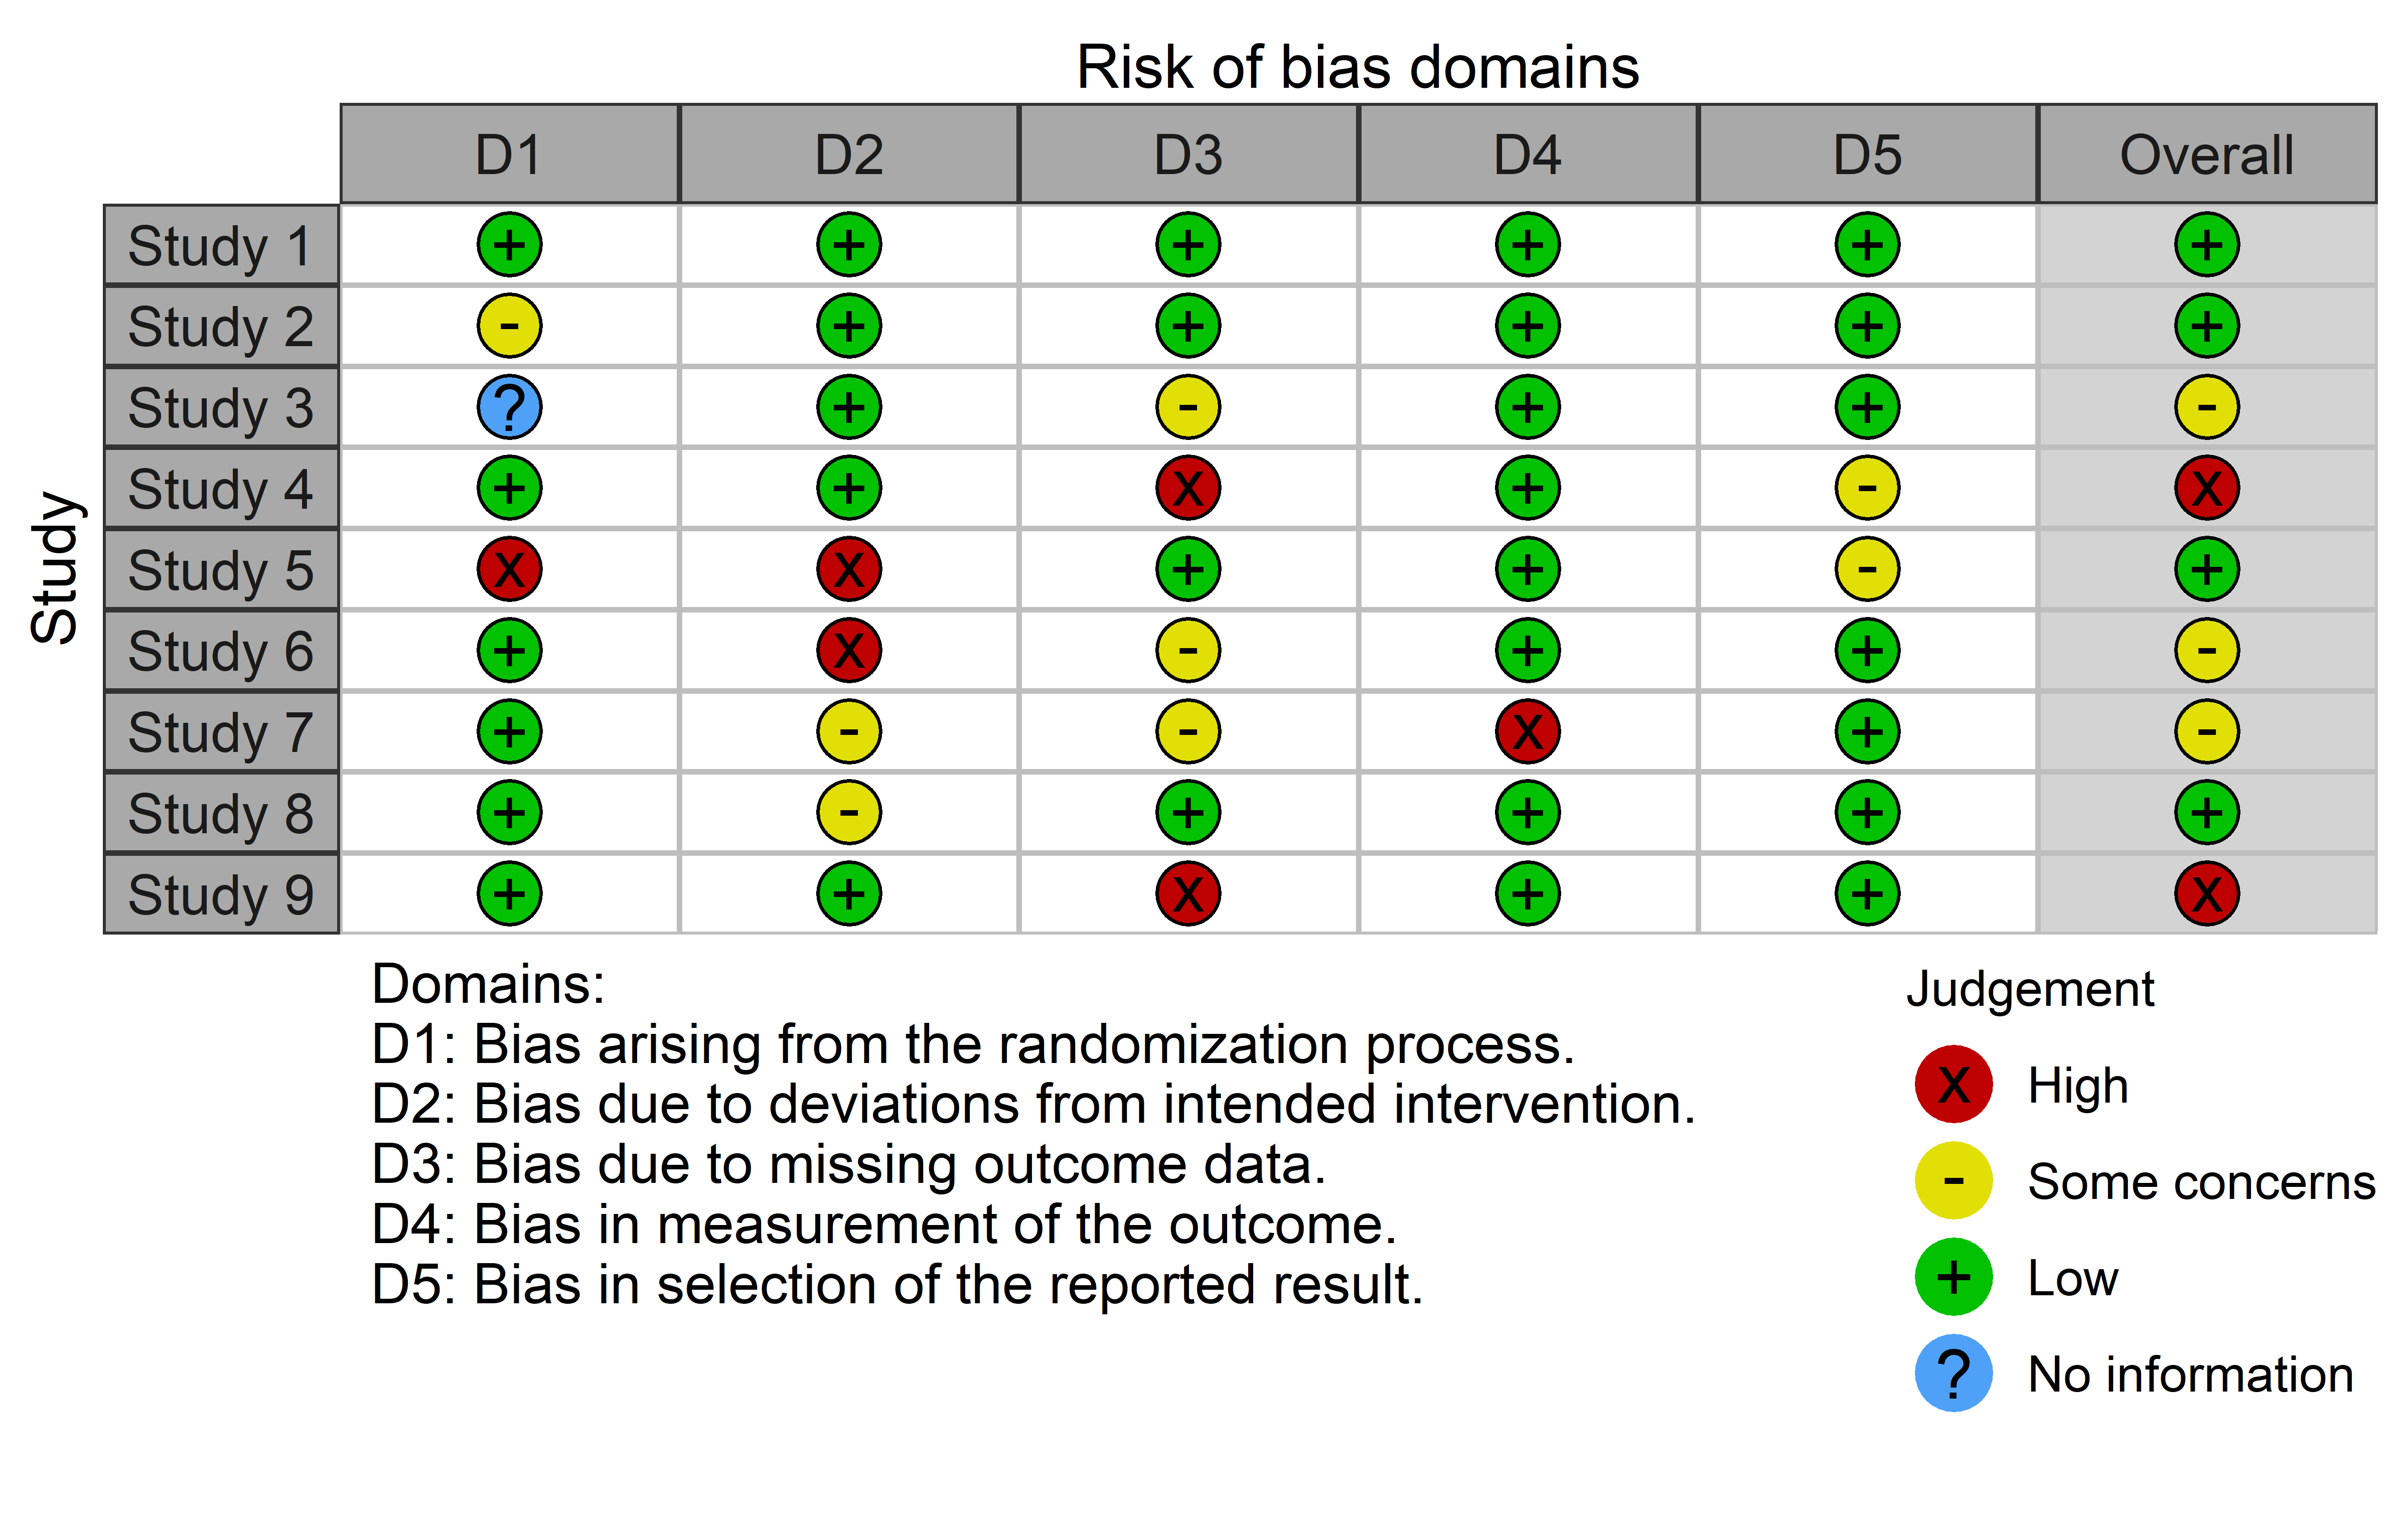
\includegraphics[width=1\linewidth]{figures/sys-rev-tools/example-rob-traffic-light-plot} \caption{Example risk of bias traffic light plot created using `robvis`}\label{fig:trafficplot}
\end{figure}

Similary, using the same data set, the summary barplot shown in Figure \ref{fig:summaryplot} is created using:

\begin{Shaded}
\begin{Highlighting}[]
\FunctionTok{rob\_summary}\NormalTok{(}\AttributeTok{data =}\NormalTok{ data\_rob2,}
            \AttributeTok{tool =} \StringTok{"ROB2"}\NormalTok{, }
            \AttributeTok{overall =} \ConstantTok{TRUE}\NormalTok{)}
\end{Highlighting}
\end{Shaded}

\begin{figure}
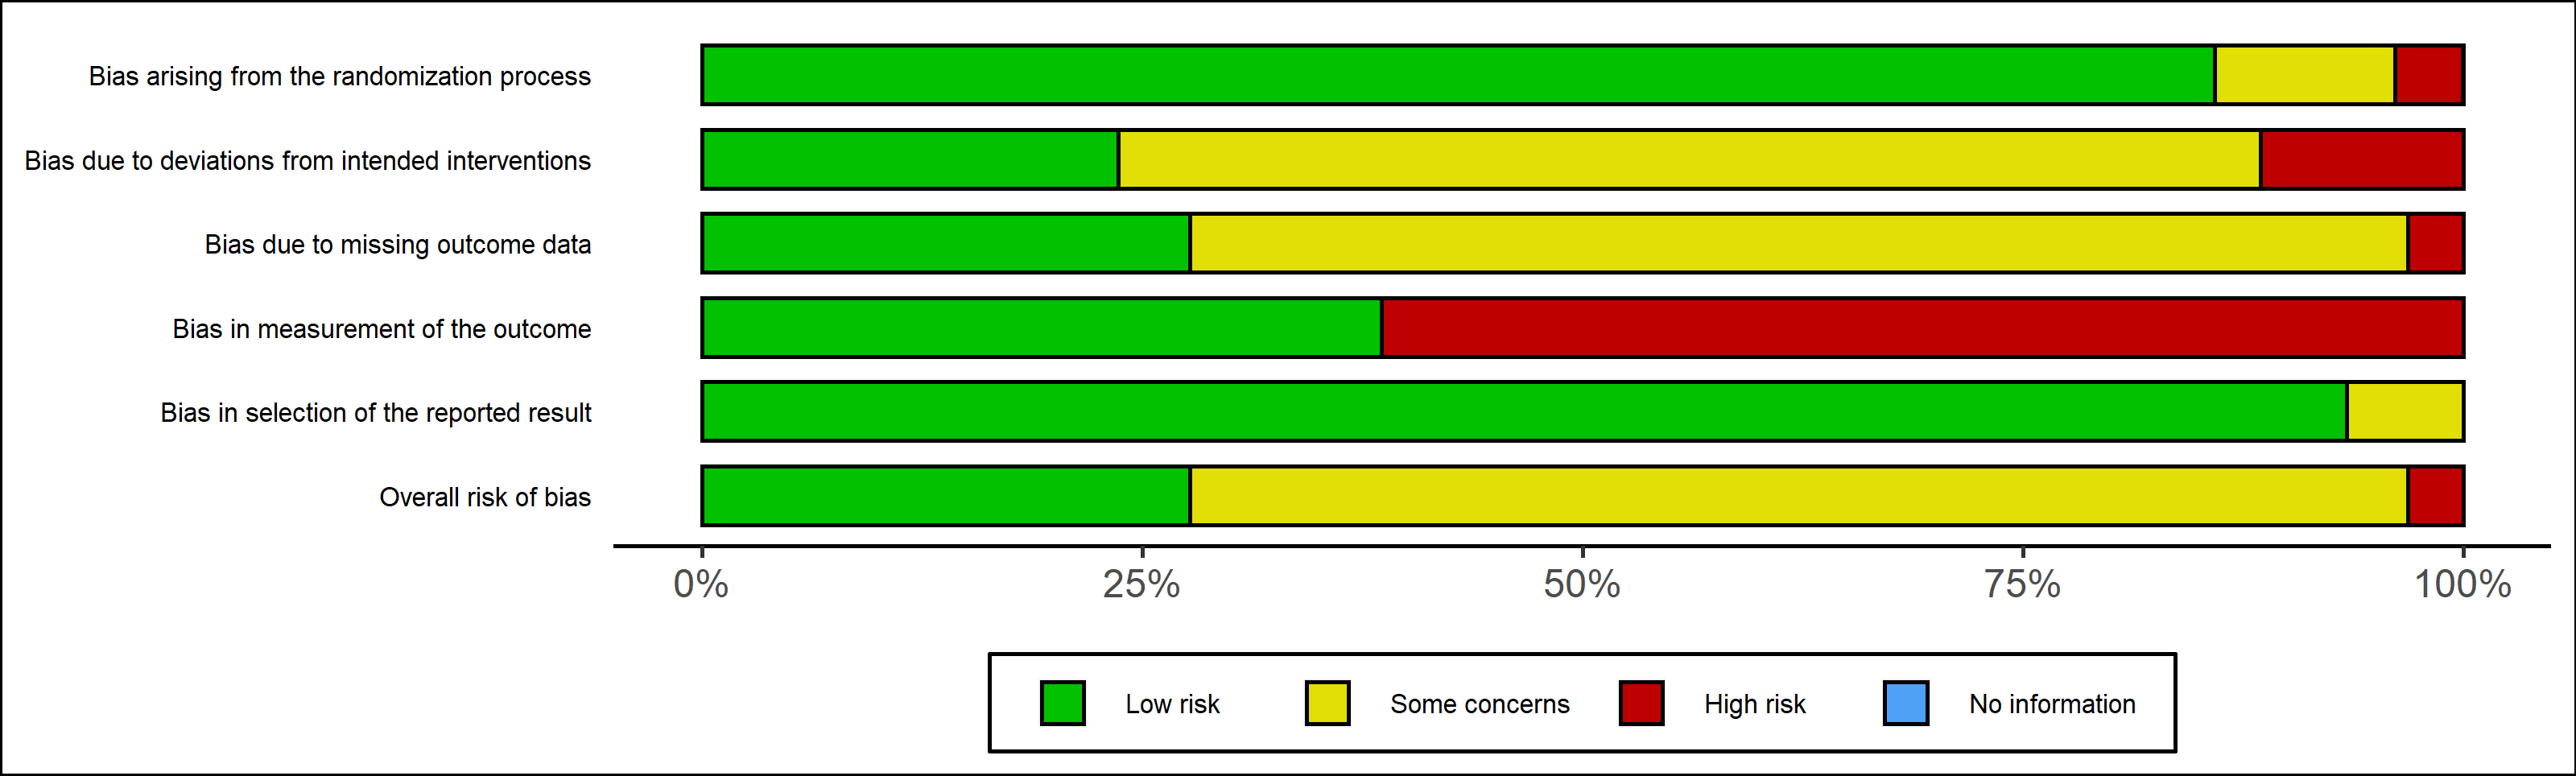
\includegraphics[width=1\linewidth]{figures/sys-rev-tools/example-rob-summary-barplot} \caption{Example risk of bias summary plot created using `robvis` and the example ROB2 dataset}\label{fig:summaryplot}
\end{figure}

A list of arguments available to the two functions in robvis are shown in Table \ref{tab:robvisarguments}

\begingroup\fontsize{9}{11}\selectfont

\begin{longtable}[t]{lcc>{\raggedright\arraybackslash}p{5cm}}
\caption{\label{tab:robvisarguments}Description of the arguments available in the two main `robvis` functions. ‘X’ indicates that the option is available for the respective function.}\\
\toprule
Argument & rob\_traffic\_light() & rob\_summary() & Description\\
\midrule
\endfirsthead
\caption[]{\label{tab:robvisarguments}Description of the arguments available in the two main `robvis` functions. ‘X’ indicates that the option is available for the respective function. \textit{(continued)}}\\
\toprule
Argument & rob\_traffic\_light() & rob\_summary() & Description\\
\midrule
\endhead

\endfoot
\bottomrule
\endlastfoot
\cellcolor{gray!6}{data} & \cellcolor{gray!6}{X} & \cellcolor{gray!6}{X} & \cellcolor{gray!6}{Defines the dataframe containing the summary (domain) level risk-of-bias assessments. See the text and Table 1 for the format expected by `robvis`}\\
tool & X & X & Defines the risk of bias assessment tool used. The RoB2 (`tool="ROB2"`), ROBINS-I (`tool="ROBINS-I"`), and QUADAS-2 (`tool="QUADAS-2"`) assessments tools are currently supported. Other tools can be visualised using the generic template (`tool = "Generic"`)\\
\cellcolor{gray!6}{colour} & \cellcolor{gray!6}{X} & \cellcolor{gray!6}{X} & \cellcolor{gray!6}{Defines the colour scheme for the plot. The default is `colour = "cochrane"` which uses the "Cochrane" (red, yellow, green) colours, while a preset option for a colour-blind friendly palette is also available (`colour = "colourblind"`). Alternatively, users can specify their own colour scheme e.g. `colour = c("\#f442c8", "\#bef441", "\#000000")`}\\
overall &  & X & Defines whether to include an additional bar showing the distibution of overall risk of bias judgements in the summary barplot figure. Default is `overall = FALSE`.\\
\cellcolor{gray!6}{weighted} & \cellcolor{gray!6}{} & \cellcolor{gray!6}{X} & \cellcolor{gray!6}{Defines whether weights should be used to produce the summary barplot figure. Default is `weighted = TRUE`, in line with current Cochrane Collaboration guidance.}\\
\addlinespace
psize & X &  & Defines the size of the points in the traffic light plot. Default is `psize = 20`.\\*
\end{longtable}
\endgroup{}

\hypertarget{reception-and-future-plans-1}{%
\subsection{Reception and Future Plans}\label{reception-and-future-plans-1}}

As of December 2021, \texttt{robvis} has been downloaded more than 13000 times. It has been well received but the systematic review community, and has been cited frequently in the published literature. A paper describing the tool was published in a special issue of Research Synthesis Methods focusing on data visualisation methods. A chapter on the tool has been incorporated in to the ``Doing Meta-Analysis in R'' online textbook.\textsuperscript{\protect\hyperlink{ref-mathias_harrer_2019_2551803}{250}}

While \texttt{robvis} is a stable package, a range of additional functionality could be added. At present, the number of tools with a specific template included in \texttt{robvis} is limited - adding additional templates is a priority. For example, a template for ROBIS, a tool for assessing risk of bias in systematic reviews, is in developement.\textsuperscript{\protect\hyperlink{ref-whiting2016robis}{251}} Additionally, the tool does not yet allow for the production of paired forest plots, where the risk-of-bias judgement is presented alongside each specific result included in the meta-analysis.\textsuperscript{\protect\hyperlink{ref-cochranechpt7}{233}} This was initially considered to be beyond the scope of the tool, as it involves the visualization of something other than risk-of-bias assessments. However, following user-driven demand, this functionality is in development and will be available in the near future. Finally, we would like to add similar functionality to that provided by the \texttt{metafor::reporter()} function, which generates a brief paragraph of text describing the results of a meta-analysis. The future \texttt{robvis::reporter()} function would provide a boilerplate description of the assessment tool used and the key domains at risk of bias.

\hypertarget{creating}{%
\section{Creating}\label{creating}}

\hypertarget{copies-of-papers-arising-from-this-thesis}{%
\section{Copies of papers arising from this thesis}\label{copies-of-papers-arising-from-this-thesis}}

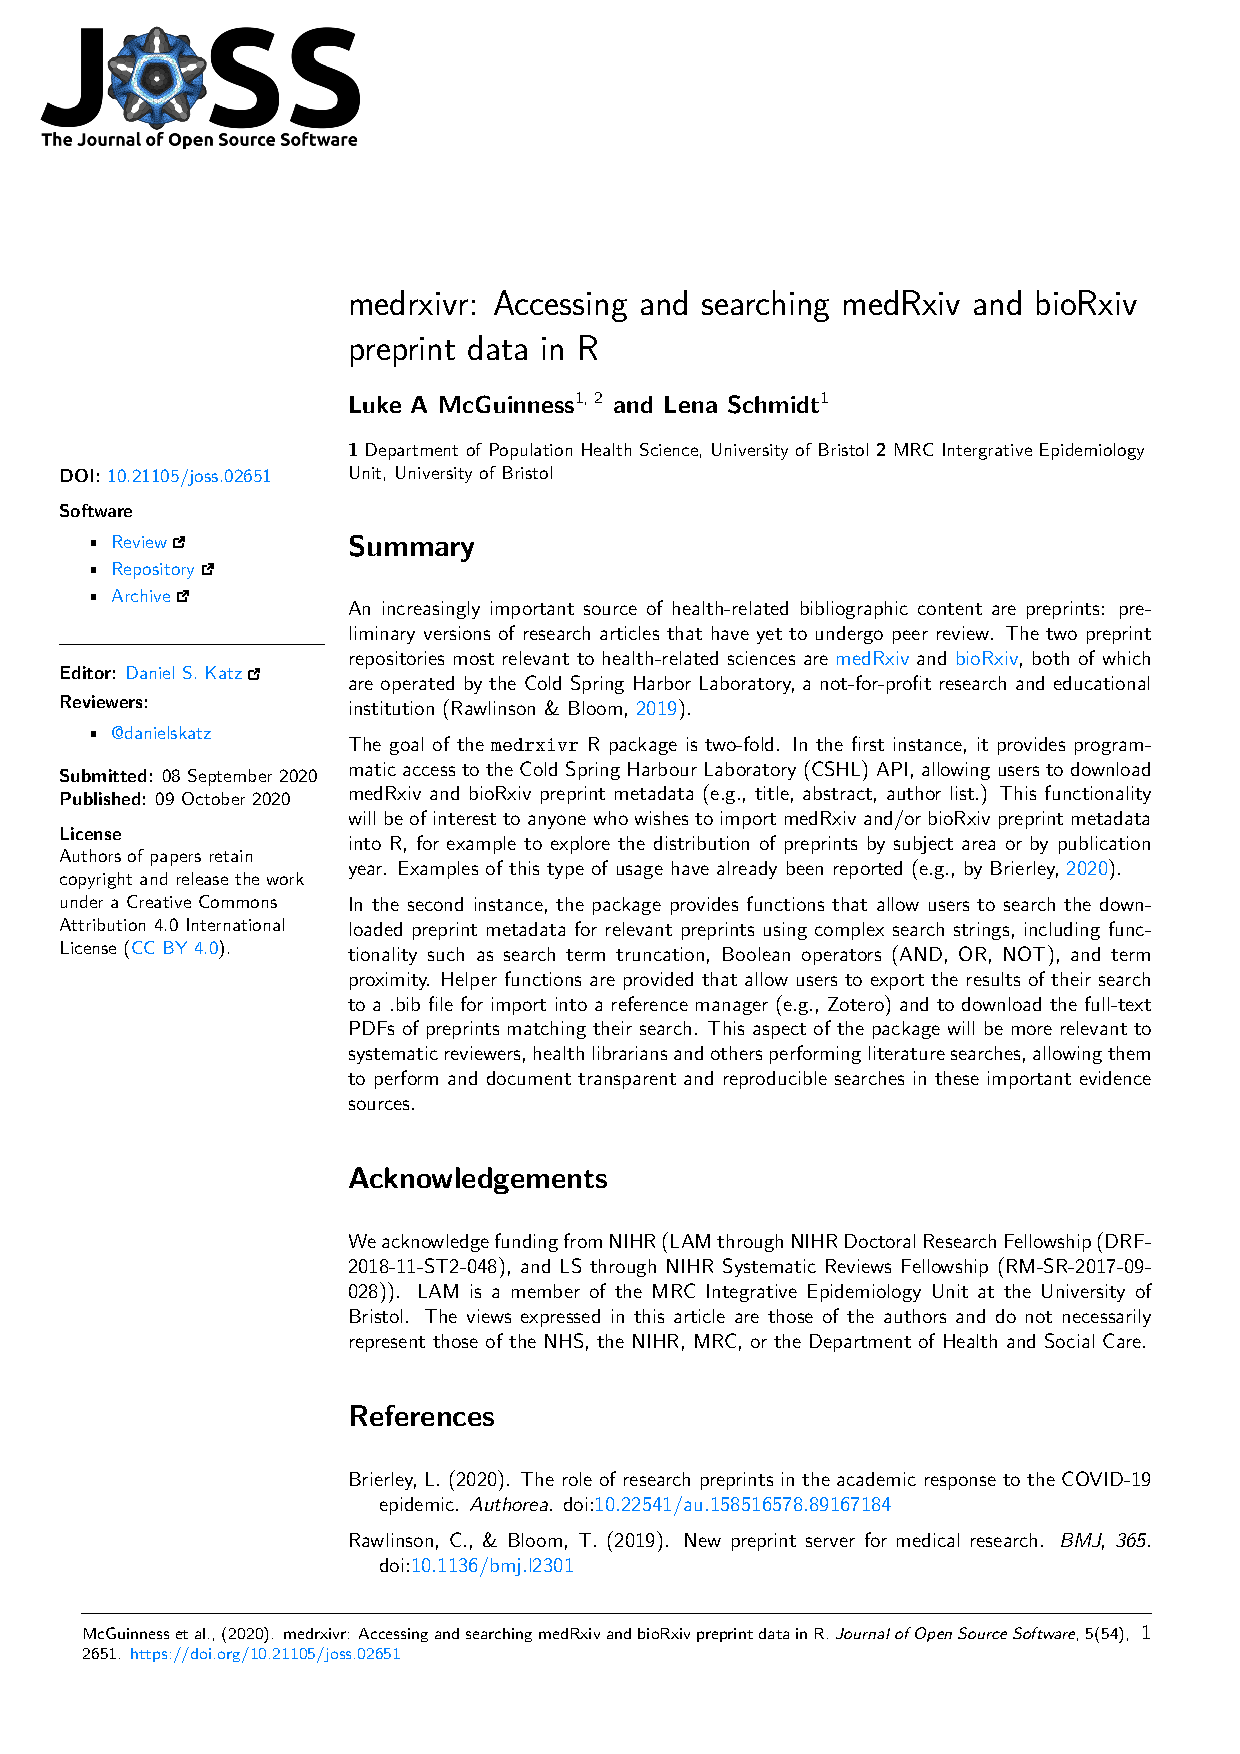
\includepdf[pages=-,pagecommand={\thispagestyle{empty}}]{published/medrxivr.pdf}
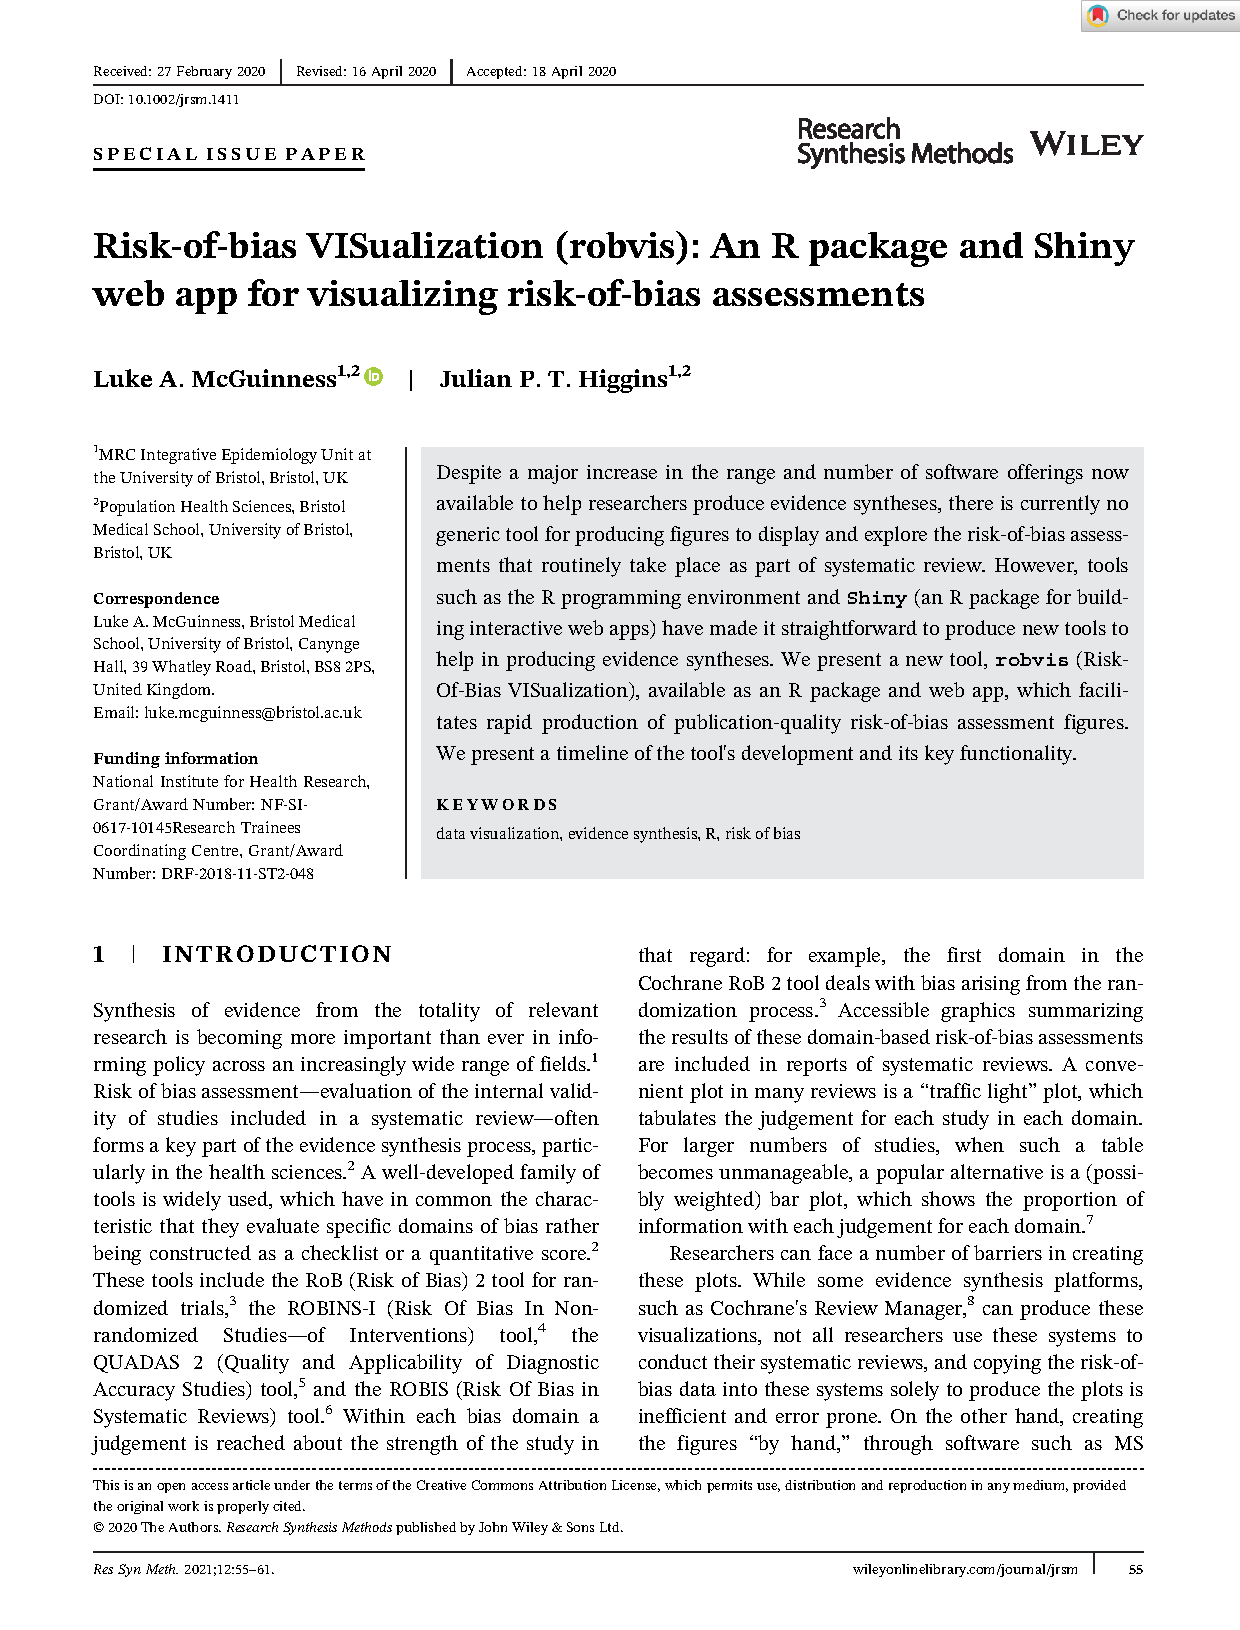
\includepdf[pages=-,pagecommand={\thispagestyle{empty}}]{published/robvis.pdf}
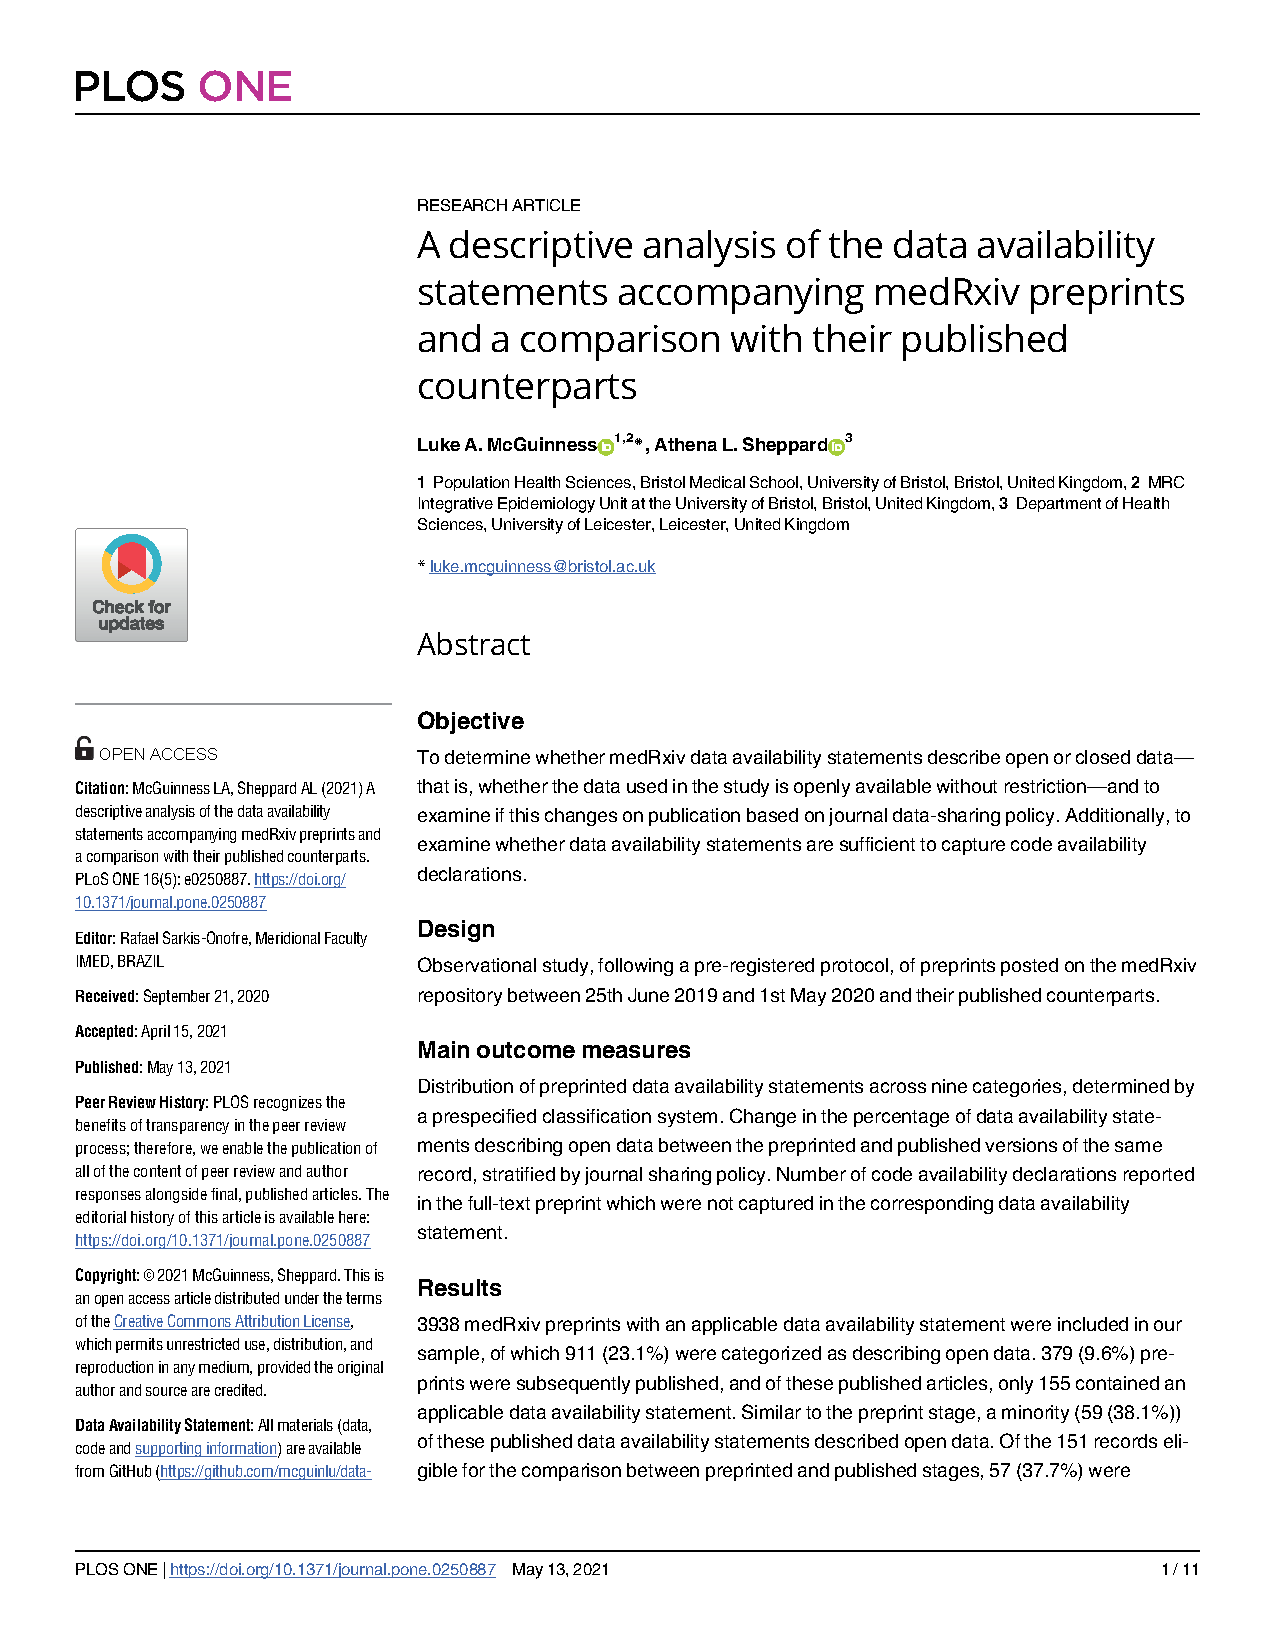
\includepdf[pages=-,pagecommand={\thispagestyle{empty}}]{published/DAS_comparison.pdf}

%%%%% REFERENCES

\setlength{\baselineskip}{0pt} % JEM: Single-space References

{\renewcommand*\MakeUppercase[1]{#1}%
\printbibliography[heading=bibintoc,title={\bibtitle}]}

\end{document}
